\chapter{Heritability Estimation}

% Need to stress that we are only calculating the narrow sense heritability
	\section{Introduction}
	The development of \glng{ldsc} has brought great prospect in estimating the heritability of complex disease for one can now estimate the heritability of a trait without requiring the rare genotype. 
	However, as noted by the author of \gls{ldsc}, when the number of causal variants were small, or when working on targeted genotype array, \gls{ldsc} tends to have a larger standard error or might produce funky results\citep{Bulik-Sullivan2015}.
	Ideally, we would like to be able to robustly estimate the heritability for all traits, disregarding the genetic architecture (e.g. number of causal \glspl{SNP}).
	
	On the other hand, it has been shown that there can be huge bias in the heritability estimation of \gls{gcta} when prevalence of a dichotomous trait is low\citep{Golan2014}.
	Although \citet{Golan2014} developed the \gls{pcgc}, which can provide robust estimation of heritability for traits with different prevalence, it still relies on the relationship matrix and therefore require the raw genotype of the samples. 
	
	Herein, we would like to develop an alternative algorithm to \gls{ldsc} for heritability estimation using only the test statistics. 
	We would also like to inspect whether if \gls{ldsc}'s heritability estimation is robust to prevalence of a trait. 
	A number of simulations were performed to compare the performance of \gls{ldsc} and our algorithm under different conditions.
	
	The work in this chapter were done in collaboration with my colleagues who have kindly provide their support and knowledges to make this piece of work possible.
	Dr Johnny Kwan, Dr Miaxin Li and Professor Sham have helped to laid the framework of this study. 
	Dr Timothy Mak has derived the mathematical proof for our heritability estimation method. 
	Miss Yiming Li, Dr Johnny Kwan, Dr Miaxin Li, Dr Timothy Mak and Professor Sham have helped with the derivation of the standard error of the heritability estimation. 
	Dr Henry Leung has provided critical suggestions on the implementation of the algorithm.
	
	\section{Methodology}	
		The overall aims of this study is to develop a robust algorithm for the estimation of the narrow sense heritability using only the summary statistic from a \gls{GWAS}.
		In \gls{GWAS}, the test statistic of a particular \gls{SNP} should be proportional to its effect size and the effect size from all the other \glspl{SNP} in \gls{LD} with it.
		Based on this property, we may use the information from the \gls{LD} matrix and the test statistic of the \gls{GWAS} \gls{SNP} the estimate the narrow sense heritability.
		
		
		\subsection{Heritability Estimation}
			Remember that the narrow-sense heritability is defined as 
			$$
				h^2 = \frac{\mathrm{Var}(X)}{\mathrm{Var}(Y)}
			$$
			where $\mathrm{Var}(X)$ is the variance of the genotype and $\mathrm{Var}r(Y)$ is the variance of the phenotype.
			In a \gls{GWAS}, regression were performed between the \glspl{SNP} and the phenotypes, giving
			\begin{equation}
				Y=\beta X+\epsilon
				\label{eq:standardRegress}
			\end{equation}
			where $Y$ and $X$ are the standardized phenotype and genotype respectively. 
			$\epsilon$ is then the error term, accounting for the non-genetic elements contributing to the phenotype (e.g. Environment factors).
			Based on \cref{eq:standardRegress}, one can then have
			\begin{align}
				\mathrm{Var}(Y) = \mathrm{Var}(\beta X)+ \mathrm{Var}(\epsilon) \nonumber\\
				\mathrm{Var}(Y) = \beta^\mathrm{Var}(X) \nonumber\\
				\beta^2\frac{\mathrm{Var}(X)}{\mathrm{Var}(Y)}= 1
				\label{eq:betaHeri}
			\end{align}
			$\beta^2$ is then considered as the portion of phenotype variance explained by the variance of genotype, which can also be considered as the narrow-sense heritability of the phenotype.
					
			A challenge in calculating the heritability from \gls{GWAS} data is that usually only the test-statistic or p-value were provided and one will not be able to directly calculate the heritability based on \cref{eq:betaHeri}. 
			In order to estimation the heritability of a trait from the \gls{GWAS} test-statistic, we first observed that when both $X$ and $Y$ are standardized, $\beta^2$ will be equal to the coefficient of determination ($r^2$). 
			Then, based on properties of the Pearson product-moment correlation coefficient:
			\begin{equation}
				r = \frac{t}{\sqrt{n-2+t^2}}
				\label{eq:pearsonProduct}
			\end{equation}
			where $t$ follows the student-t distribution and $n$ is the number of samples, one can then obtain the $r^2$ by taking the square of \cref{eq:pearsonProduct}
			\begin{equation}
				r^2 = \frac{t^2}{n-2+t^2}
				\label{eq:oriRSquared}
			\end{equation}
			It is observed that $t^2$ will follow the F-distribution.
			When $n$ is big, $t^2$ will converge into $\chi^2$ distribution.
			
			Furthermore, when the effect size is small and $n$ is big, $r^2$ will be approximately $\chi^2$ distributed with mean $\sim 1$. 
			We can then approximate \cref{eq:oriRSquared} as
			\begin{equation}
				r^2= \frac{\chi^2}{n}
				\label{eq:approxChi}
			\end{equation}
			and define the \emph{observed} effect size of each \gls{SNP} to be
			\begin{equation}
			f=\frac{\chi^2-1}{n}
			\label{eq:observedEffect}
			\end{equation}
			
			When there are \gls{LD} between each individual \glspl{SNP}, the situation will become more complicated as each \glspl{SNP}' observed effect will contains effect coming from other \glspl{SNP} in \gls{LD} with it:
			\begin{equation}
			f_{observed} = f_{true}+f_{LD}
			\label{eq:conceptF}
			\end{equation}
			
			To account for the \gls{LD} structure, we first assume our phenotype $\boldsymbol{Y}$ and genotype $\boldsymbol{X}=(X_1,X_2,\dots,X_m)^t$ are standardized and that
			\begin{align*}
				\boldsymbol{Y}\sim f(0,1) \\
				\boldsymbol{X}\sim f(0,\boldsymbol{R})
			\end{align*}
			Where $\boldsymbol{R}$ is the \gls{LD} matrix between \glspl{SNP}.
			
			We can then express \cref{eq:standardRegress} in matrix form:
			\begin{align}
				\boldsymbol{Y}=\boldsymbol{\beta}^t\boldsymbol{X}+\epsilon
				\label{eq:matrixRegress}
			\end{align}
			Because the phenotype is standardized with variance of 1, the narrow sense heritability can then be expressed as
			\begin{align}
				Heritability& = \frac{\mathrm{Var}(\boldsymbol{\beta}^t\boldsymbol{X})}{\mathrm{Var}(\boldsymbol{Y})} \nonumber\\
				&=\mathrm{Var}(\boldsymbol{\beta}^t\boldsymbol{X})
			\end{align}
			If we then assume now that $\boldsymbol{\beta} = (\beta_1, \beta_2,\dots,\beta_m)^t$ has distribution
			\begin{align*}
				\boldsymbol{\beta}&\sim f(0,\boldmath{H})\\
				\boldsymbol{H}&=diag(\boldsymbol{h})\\
				\boldsymbol{h}&=(h_1^2,h_2^2,\dots,h_m^2)^t
			\end{align*}
			where $\boldsymbol{H}$ is the variance of the ``true'' effect. 
			It is shown that heritability can be expressed as %The later part was gone because that will contains E(\beta) which = 0
			\begin{align}
			\mathrm{Var}(\boldsymbol{\beta}^t\boldsymbol{X}) &= \mathrm{E}_X\mathrm{Var}_{\beta|X}(\boldsymbol{X}^t\boldsymbol{\beta})+\mathrm{Var}_X\mathrm{E}_{(\beta|X)}(\boldsymbol{\beta}^2\boldsymbol{X}) \nonumber\\
			&=\mathrm{E}_X(\boldsymbol{X}^t\boldsymbol{\beta\beta}^T\boldsymbol{X}) \nonumber\\ 
			&= \mathrm{E}_X(\boldsymbol{X}^t\boldsymbol{HX}) \nonumber\\
			&= \mathrm{E}(\boldsymbol{X})^t\boldsymbol{H}\mathrm{E}(\boldsymbol{X})+\mathrm{Tr}(\mathrm{Var}(\boldsymbol{X}\boldsymbol{H})) \nonumber\\
			&=\mathrm{Tr}(\mathrm{Var}(\boldsymbol{X}\boldsymbol{H})) \nonumber\\
			&=\sum_ih_i^2
			\label{eq:proveHerit}
			\end{align}
			
			Now if we consider the covariance between \gls{SNP} i ($\boldsymbol{X_i}$) and $\boldsymbol{Y}$, we have
			\begin{align}
			 \mathrm{Cov}(\boldsymbol{X}_i,\boldsymbol{Y}) &= \mathrm{Cov}(\boldsymbol{X}_i,\boldsymbol{\beta}^t\boldsymbol{X}+\epsilon) \nonumber\\
			 &=\mathrm{Cov}(\boldsymbol{X}_i,\boldsymbol{\beta}^t\boldsymbol{X}) \nonumber\\
			 &=\sum_j{\mathrm{Cov}(\boldsymbol{X}_i,\boldsymbol{X}_j)\boldsymbol{\beta}_j} \nonumber\\
			 &=\boldsymbol{R}_i\boldsymbol{\beta}_j
			 \label{eq:covPhenoTrue}
			\end{align}
			
			As both $\boldsymbol{X}$ and $\boldsymbol{Y}$ are standardized, the covariance will equal to the correlation and we can define the correlation between \gls{SNP} i and $Y$ as
			\begin{equation}
				\rho_i = \boldsymbol{R}_i\boldsymbol{\beta}_j
				\label{eq:corPhenoTrue}
			\end{equation}
			In reality, the \emph{observed} correlation usually contains error. 
			Therefore we define the \emph{observed} correlation between SNP$_i$ and the phenotype($\hat{\rho_i}$) to be
			\begin{equation}
			\hat{\rho_i} = \rho_i+\frac{\epsilon_i}{\sqrt{n}}
			\label{eq:obsPheno}
			\end{equation}
			for some error $\epsilon_i$. 
			The distribution of the correlation coefficient about the true correlation $\rho$ is approximately
			$$
				\hat{\rho_i}\sim f(\rho_i, \frac{(1-\rho^2)^2}{n})
			$$
			By making the assumption that $\rho_i$ is close to 0 for all $i$, we have 
			\begin{align*}
				\mathrm{E}(\epsilon_i|\rho_i)&\sim 0\\
				\mathrm{Var}(\epsilon_i|\rho_i)&\sim 1
			\end{align*}
			We then define our $z$-statistic and $\chi^2$-statistic as
			\begin{align*}
				z_i &= \hat{\rho_i}\sqrt{n} \\
				\chi^2 &= z_i^2\\
				&=\hat{\rho_i}^2n
			\end{align*}
			From \cref{eq:obsPheno} and \cref{eq:corPhenoTrue}, $\chi^2$ can then be expressed as
			\begin{align*}
			\chi^2&=\hat{\rho}^2n\\
			&=n(\boldsymbol{R}_i\boldsymbol{\beta}_j+\frac{\epsilon_i}{\sqrt{n}})^2
			\end{align*}
			The expectation of $\chi^2$ is then
			\begin{align*}
			\mathrm{E}(\chi^2) &= n(\boldsymbol{R}_i\boldsymbol{\beta\beta}^t\boldsymbol{R}_i+2\boldsymbol{R}_i\boldsymbol{\beta}\frac{\epsilon_i}{\sqrt{n}}+\frac{\epsilon_i^2}{n}) \\
			&= n\boldsymbol{R}_i\boldsymbol{H}\boldsymbol{R}_i+1
			\end{align*}
			To derive least square estimates of $h_i^2$, we need to find $\hat{h_i^2}$ which minimizes
			\begin{align*}
				\sum_i(\chi_i^2-\mathrm{E}(\chi_i^2))^2&=\sum_i(\chi_i^2-(n\boldsymbol{R}_i\boldsymbol{H}\boldsymbol{R}_i+1))^2 \\
				&=\sum_i(\chi_i^2-1-n\boldsymbol{R}_i\boldsymbol{H}\boldsymbol{R}_i)^2 
			\end{align*}
			If we define 
			\begin{equation}
			f_i= \frac{\chi_i^2-1}{n}
			\label{eq:defineF}
			\end{equation}
			we got
			\begin{align}
			\sum_i(\chi_i^2-\mathrm{E}(\chi_i^2))^2&=\sum_i(f_i-\boldsymbol{R}_i\boldsymbol{H}\boldsymbol{R}_i)^2 \nonumber\\
			&=\boldsymbol{ff}^t-2\boldsymbol{f}^t\boldsymbol{R_{sq}\hat{h}}+\boldsymbol{\hat{h}}^t\boldsymbol{R_{sq}}^t\boldsymbol{R_{sq}\hat{h}}
			\label{eq:leastSquareH}
			\end{align}
			where $\boldsymbol{R_{sq}} = \boldsymbol{R}\circ\boldsymbol{R}$.
			By differentiating \cref{eq:leastSquareH} w.r.t $\hat{h}$ and set to 0, we get
			\begin{align}
				2\boldsymbol{R_{sq}}^t\boldsymbol{R_{sq}}\boldsymbol{\hat{h^2}}-2\boldsymbol{R_{sq}f}&=0 \nonumber\\
				\boldsymbol{R_{sq}}\boldsymbol{\hat{h^2}} &=\boldsymbol{f}
				\label{eq:shrekEq}
			\end{align}
			And the heritability is then defined as 
			\begin{equation}
			\hat{Heritability} = \boldsymbol{1}^t\boldsymbol{R_{sq}}^{-1}\boldsymbol{f}
			\label{eq:fullShrek}
			\end{equation}
		\subsection{Calculating the \Glng{se}}
			From \cref{eq:fullShrek}, we can derive the variance of heritability $H$ as 
			\begin{align}
				\mathrm{Var}(H) &= \mathrm{E}[H^2]-\mathrm{E}[H]^2\nonumber\\
				&=\mathrm{E}[(\boldsymbol{1}^t\boldsymbol{R_{sq}}^{-1}\boldsymbol{f})^2]-\mathrm{E}[\boldsymbol{1}^t\boldsymbol{R_{sq}}^{-1}\boldsymbol{f}](\mathrm{E}[\boldsymbol{1}^t\boldsymbol{R_{sq}}^{-1}\boldsymbol{f}])^t \nonumber \\
				&=\mathrm{E}[\boldsymbol{1}^t\boldsymbol{R_{sq}}^{-1}\boldsymbol{ff}^t\boldsymbol{R_{sq}}^{-1}\boldsymbol{1}]-\mathrm{E}[\boldsymbol{1}^t\boldsymbol{R_{sq}}^{-1}\boldsymbol{f}](\mathrm{E}[\boldsymbol{1}^t\boldsymbol{R_{sq}}^{-1}\boldsymbol{f}])^t \nonumber \\
				&=\boldsymbol{1}^t\boldsymbol{R_{sq}}^{-1}\mathrm{E}[\boldsymbol{ff}^t]\boldsymbol{R_{sq}}^{-1}\boldsymbol{1}-\mathrm{E}[\boldsymbol{1}^t\boldsymbol{R_{sq}}^{-1}\boldsymbol{f}](\mathrm{E}[\boldsymbol{1}^t\boldsymbol{R_{sq}}^{-1}\boldsymbol{f}])^t \nonumber \\
				&=\boldsymbol{1}^t\boldsymbol{R_{sq}}^{-1}\mathrm{Var}(\boldsymbol{f})\boldsymbol{R_{sq}}^{-1}\boldsymbol{1}+\mathrm{E}[\boldsymbol{1}^t\boldsymbol{R_{sq}}^{-1}\boldsymbol{f}](\mathrm{E}[\boldsymbol{1}^t\boldsymbol{R_{sq}}^{-1}\boldsymbol{f}])^t-\mathrm{E}[\boldsymbol{1}^t\boldsymbol{R_{sq}}^{-1}\boldsymbol{f}](\mathrm{E}[\boldsymbol{1}^t\boldsymbol{R_{sq}}^{-1}\boldsymbol{f}])^t \nonumber\\
				&=\boldsymbol{1}^t\boldsymbol{R_{sq}}^{-1}\mathrm{Var}(\boldsymbol{f})\boldsymbol{R_{sq}}^{-1}\boldsymbol{1}
				\label{eq:varHvarf}
			\end{align}
			Therefore, to obtain the variance of $H$, we first need to calculate the variance covariance matrix of $\boldsymbol{f}$.
			
			We first consider the standardized genotype $X_i$ with standard normal mean $z_i$ and non-centrality parameter
			$\mu_i$, we have
			\begin{align*}
				\mathrm{E}[X_i]&=\mathrm{E}[z_i+\mu_i]\\
				&=\mu_i\\
				\mathrm{Var}(X_i) &=\mathrm{E}[(z_i+\mu_i)^2]+\mathrm{E}[(z_i+\mu_i)]^2\\
				&=\mathrm{E}[z_i^2+\mu_i^2+2z_i\mu_i]+\mu_i^2\\
				&=1 \\
				\mathrm{Cov}(X_i,X_j)&=\mathrm{E}[(z_i+\mu_i)(z_j+\mu_j)]-\mathrm{E}[z_i+\mu_i]\mathrm{E}[z_j+\mu_j]\\
				&=\mathrm{E}[z_iz_j+z_i\mu_j+\mu_iz_j+\mu_i\mu_j]-\mu_i\mu_j\\
				&=\mathrm{E}[z_iz_j]+\mathrm{E}[z_i\mu_j]+\mathrm{E}[z_j\mu_i]+\mathrm{E}[\mu_i\mu_j]-\mu_i\mu_j\\
				&=\mathrm{E}[z_iz_j]
			\end{align*}
			As the genotypes are standardized, therefore $\mathrm{Cov}(X_i,X_j)==\mathrm{Cor}(X_i,X_j)$, we can obtain
			$$
				\mathrm{Cov}(X_i,X_j)=\mathrm{E}[z_iz_j]=R_{ij}
			$$
			where $R_{ij}$ is the \gls{LD} between \gls{SNP}$_i$ and \gls{SNP}$_j$.
			Given these information, we can then calculate $\mathrm{Cov}(\chi_i^2,\chi_j^2)$ as:
			\begin{align*}
				\mathrm{Cov}(X_i^2,X_j^2)=&\mathrm{E}[(z_i+\mu_i)^2(z_j+\mu_j)^2]-\mathrm{E}[z_i+\mu_i]\mathrm{E}[z_j+\mu_j]\\
				=&\mathrm{E}[(z_i^2+\mu_i^2+2z_i\mu_i)(z_j^2+\mu_j^2+2z_j\mu_j)] \\
				&-\mathrm{E}[z_i^2+\mu_i^2+2z_i\mu_i]\mathrm{E}[z_j^2+\mu_j^2+2z_j\mu_j]\\
				=&\mathrm{E}[(z_i^2+\mu_i^2+2z_i\mu_i)(z_j^2+\mu_j^2+2z_j\mu_j)]\\
				&-(\mathrm{E}[z_i^2]+\mathrm{E}[\mu_i^2]+2\mathrm{E}[z_i\mu_i])(\mathrm{E}[z_j^2]+\mathrm{E}[\mu_j^2]+2\mathrm{E}[z_j\mu_j])\\
				=&\mathrm{E}[z_i^2(z_j^2+\mu_j^2+2z_j\mu_j)+\mu_i^2(z_j^2+\mu_j^2+2z_j\mu_j)+2z_i\mu_i(z_j^2+\mu_j^2+2z_j\mu_j)]\\
				&-(1+\mu_i^2)(1+\mu_j^2)\\
				=&\mathrm{E}[z_i^2(z_j^2+\mu_j^2+2z_j\mu_j)]+\mu_i^2\mathrm{E}[z_j^2+\mu_j^2+2z_j\mu_j]\\
				&+2\mu_i\mathrm{E}[z_i(z_j^2+\mu_j^2+2z_j\mu_j)]-(1+\mu_i^2)(1+\mu_j^2)\\
				=&\mathrm{E}[z_i^2z_j^2+z_i^2\mu_j^2+2z_i^2z_j\mu_j]+\mu_i^2+\mu_i^2\mu_j^2\\
				&+2\mu_i\mathrm{E}[z_iz_j^2+z_i\mu_j^2+2z_iz_j\mu_j]-(1+\mu_i^2)(1+\mu_j^2)\\
				=&\mathrm{E}[z_i^2z_j^2]+\mu_j^2+\mu_i^2+\mu_i^2\mu_j^2+4\mu_i\mu_j\mathrm{E}[z_iz_j]-(1+\mu_i^2+\mu_j^2+\mu_i\mu_j)\\
				=&\mathrm{E}[z_i^2z_j^2]+4\mu_i\mu_j\mathrm{E}[z_iz_j]-1
			\end{align*}
			Remember that $\mathrm{E}[z_iz_j] = R_{ij}$, we then have
			$$
				\mathrm{Cov}(X_i^2, X_j^2)=\mathrm{E}[z_i^2z_j^2]+4\mu_i\mu_jR_{ij}-1
			$$
			By definition, 
			$$
				z_i|z_j\sim N(\mu_i+R_{ij}(z_j-\mu_j),1-R_{ij}^2)
			$$
			We can then calculate $\mathrm{E}[z_i^2z_j^2]$ as
			\begin{align*}
				\mathrm{E}[z_i^2z_j^2]&=\mathrm{Var}[z_iz_j]+\mathrm{E}[z_iz_j]^2\\
				&=\mathrm{E}[\mathrm{Var}(z_iz_j|z_i)]+\mathrm{Var}[\mathrm{E}[z_iz_j|z_i]]+R_{ij}^2\\
				&=\mathrm{E}[z_j^2\mathrm{Var}(z_i|z_j)]+\mathrm{Var}[z_j\mathrm{E}[z_i|z_j]]+R_{ij}^2\\
				&=(1-R_{ij}^2)\mathrm{E}[z_j^2]+\mathrm{Var}(z_j(\mu_i+R_{ij}(z_j-\mu_j)))+R_{ij}^2\\
				&=(1-R_{ij}^2)+\mathrm{Var}(z_j\mu_i+R_{ij}z_j^2-\mu_jz_jR_{ij})+R_{ij}^2\\
				&=1+\mu_i^2\mathrm{Var}(z_j)+R_{ij}^2\mathrm{Var}(z_j^2)-\mu_j^2R_{ij}^2\mathrm{Var}(z_j)\\
				&=1+2R_{ij}^2
			\end{align*}
			As a result, the variance covariance matrix of the $\chi^2$ variances represented as
			\begin{equation}
				\mathrm{Cov}(X_i^2,X_j^2) = 2R_{ij}^2+4R_{ij}\mu_i\mu_j
				\label{eq:finalChi}
			\end{equation}
			As we only have the \emph{observed} expectation, we should re-define \cref{eq:finalChi} as
			\begin{equation}
				\mathrm{Cov}(X_i^2,X_j^2) = \frac{2R_{ij}^2+4R_{ij}\mu_i\mu_j}{n^2}
				\label{eq:finalChiCov}
			\end{equation}
			where $n$ is the sample size.
			
			By substituting \cref{eq:finalChiCov} into \cref{eq:varHvarf}, we will get
			\begin{align}
				\mathrm{Var}(H) &=\boldsymbol{1}^t\boldsymbol{R_{sq}}^{-1}\frac{2\boldsymbol{R_{sq}}+4\boldsymbol{R}\circ \boldsymbol{zz}^t}{n^2}\boldsymbol{R_{sq}}^{-1}\boldsymbol{1}
				\label{eq:covH}
			\end{align}
			where $\boldsymbol{z} = \sqrt{\boldsymbol{\chi^2}}$ from \cref{eq:defineF}, with the direction of effect as its sign and $\circ$ is the element-wise product (Hadamard product).
			 
			The problem with \cref{eq:covH} is that it requires the direction of effect. 
			Without the direction of effect, the estimation of \gls{se} will be inaccurate. 
			If we consider that $\boldsymbol{f}$ is approximately $\chi^2$ distributed, we might view \cref{eq:shrekEq} as a decomposition of a vector of $\chi^2$ distributions with degree of freedom of 1. 
			Replacing the vector $\boldsymbol{f}$ with a vector of 1, we can perform the decomposition of the degree of freedom, getting the ``effective number''($e$) of the association\citep{Li2011}. 
			%The problem of this effective number is that they uses the eigenvalue instead of this multiplication.
			%So either we have to explain why we don't follow it (therefore explaining the slidding windows) or we should just avoid mentioning the effective number
			Substituting $e$ into the variance equation of non-central $\chi^2$ distribution will yield
			\begin{equation}
			\mathrm{Var}(H) = \frac{2(e+2H)}{n^2}
			\label{eq:effectiveChi}
			\end{equation}
			\cref{eq:effectiveChi} should in theory gives us an heuristic estimation of the \gls{se}. 
			Moreover, the direction of effect was not required for \cref{eq:effectiveChi}, reducing the number of input required from the user.
		\subsection{Case Control Studies}	 
		%Discuss on the liability threshold model. Then the apply orange paper. Then explain how to get the results. 
			When dealing with case control data, as the phenotype were usually discontinuous, we cannot directly use \cref{eq:fullShrek} to estimate the heritability.
			Instead, we will need to employ the concept of liability threshold model from \cref{sec:liability}. 
			
			Based on the derivation of \citet{Yang2010}, the approximate ratio between the \gls{ncp} obtained from case control studies ($NPC_{CC}$) and quantitative trait studies($NCP_{QT}$) were
		
			\begin{equation}
			\frac{NCP_{CC}}{NCP_{QT}} = \frac{i^2v(1-v)N_{CC}}{(1-K)^2N_{QT}}
			\label{eq:originNCPTransform}
			\end{equation}
			where
			\begin{align*}
			 K &= \text{Population Prevalence} \\
			 v &= \text{Proportion of Cases}\\
			 N &= \text{Total Number of Samples}\\
			 i &= \frac{z}{K}\\
			 z &= \text{height of standard normal curve at truncation pretained to K}
			\end{align*}
			
			Using this approximation deviated by \citet{Yang2010}, we can directly transform the \gls{ncp} between the case control studies and quantitative trait studies.
			As we were transforming the \gls{ncp} of a single study, the $N_{CC}$ and $N_{QT}$ will be the same, therefore \cref{eq:originNCPTransform} became
			\begin{equation}
			NCP_{QT} = \frac{NCP_{CC}(1-K)^2}{i^2v(1-v)}
			\label{eq:transform}
			\end{equation}
			
			By combining \cref{eq:transform} and \cref{eq:defineF}, we can then have
			\begin{equation}
			f = \frac{(\chi^2_{CC}-1)(1-K)^2}{ni^2v(1-v)}
			\end{equation}
			where $\chi^2_{CC}$ is the test statistic from the case control association test.
			Finally, the heritability estimation of case control studies can be simplified to 
			\begin{equation}
			\hat{Heritability} =\frac{(1-K)^2}{i^2v(1-v)} \boldsymbol{1}^t\boldsymbol{R_{sq}}^{-1}\boldsymbol{f}
			\label{eq:caseControlHerit}
			\end{equation}
			
		\subsection{Extreme Phenotype Selections}
			%Explain why we perform extreme phenotype selections. Explain how that affect the variance of the estimation. Finally, explain how to perform heritability estimation on extreme phenotype. 
			When extreme phenotype selection were performed, the variance of the selected phenotype will not be representative of that in the population.
			Most notably, the variance of the post selection phenotype will tends to increase.
			Thus, to adjust for this bias, one can multiple the estimated heritability $\hat{h^2}$ by the ratio between the variance before $V_P$ and after $V_{P'}$ the selection process\citep{Sham2014}:
			
			\begin{equation}
			\hat{Heritability} = \frac{V_{P'}}{V_P}\boldsymbol{1}^t\boldsymbol{R_{sq}}^{-1}\boldsymbol{f}
			\label{eq:extremeShrek}
			\end{equation}
			
		\subsection{Calculating the \glsentrylong{LD} matrix}
			% Might want to remove this section as we no longer use this correction
			To estimate the heritability, the population \gls{LD} matrix is required.
			In reality, one can only obtain the \gls{LD} matrix based on a subset of the population (e.g. the 1000 genome project\citep{Project2012} or the HapMap project\citep{Altshuler2010}).
			There are therefore sampling errors among the \gls{LD} elements. 
			
			Now if we consider \cref{eq:fullShrek}, the $\boldsymbol{R_{sq}}$ matrix is required.
			As the squared \gls{LD} is used, a positive bias is induced into our $\boldsymbol{R_{sq}}$ matrix. 
			
			Based on \citet{Shieh2010}, one can correct for bias in the Pearson correlation $\rho$ using
			\begin{equation}
			\rho = \rho\{1+\frac{1-\rho^2}{2(N-4)}\}
			\label{eq:rhoCorrect}
			\end{equation}
			where $N$ is the number of sample used in the calculation of $\rho$. 
			Similarly, there exists a bias correction equation for $\rho^2$:
			\begin{equation}
				\rho^2=1-\frac{N-3}{N-2}(1-\rho^2)\{1+\frac{2(1-\rho^2)}{N-3.3}\}
				\label{eq:rho2Correct}
			\end{equation}
			Therefore, we corrected the $\boldsymbol{R_{sq}}$ based on \cref{eq:rho2Correct} such that the bias in estimation can be minimized. 
		\subsection{Inverse of the \glsentrylong {LD} matrix}
			In order to obtain the heritability estimation, we will require to solve \cref{eq:fullShrek}. 
			If $\boldsymbol{R_{sq}}$ is of full rank and positive semi-definite, it will be straight-forward to solve the matrix equation.
			However, more often than not, the \gls{LD} matrix are rank-deficient and suffer from multicollinearity, making it ill-conditioned, therefore highly sensitive to changes or errors in the input.
			To be exact, we can view \cref{eq:fullShrek} as calculating the sum of $\boldsymbol{\hat{h^2}}$ from  \cref{eq:shrekEq}.
			This will involve solving for
			\begin{equation}
			\boldsymbol{\hat{h^2}} = \boldsymbol{R_{sq}}^{-1}\boldsymbol{f}
			\label{eq:shrekInverse}
			\end{equation}
			where an inverse of $\boldsymbol{R_{sq}}$ is observed. 
			
			In normal circumstances (e.g. when $\boldsymbol{R_{sq}}$ is full rank and positive semi-definite), one can easily solve \cref{eq:shrekInverse} using the QR decomposition or LU decomposition.
			However, when $\boldsymbol{R_{sq}}$ is ill-conditioned, the traditional decomposition method will fail.
			Even if the decomposition is successfully performed, the result tends to be a meaningless approximation to the true $\boldsymbol{\hat{h^2}}$. 
			
			Therefore, to obtain a meaningful solution, regularization techniques such as the Tikhonov Regularization (also known as Ridge Regression) and \gls{tSVD} has to be performed\citep{Neumaier1998}. 
			There are a large variety of regularization techniques, yet the discussion of which is beyond the scope of this study. 
			In this study, we will focus on the use of \gls{tSVD} in the regularization of the \gls{LD} matrix.
			This is because the \gls{SVD} routine has been implemented in the EIGEN C++ library \citep{eigenweb}, allowing us to implement the \gls{tSVD} method without much concern with regard to the detail of the algorithm. 
			
			To understand the problem of the ill-conditioned matrix and regularization method, we consider the matrix equation $\boldsymbol{Ax}=\boldsymbol{B}$ where $\boldsymbol{A}$ is ill-conditioned or singular with $n\times n$ dimension.
			The \gls{SVD} of $\boldsymbol{A}$ can be expressed as 
			\begin{align}
				\boldsymbol{A} = \boldsymbol{U\Sigma V}^t
				\label{eq:svd}
			\end{align}
			where $\boldsymbol{U}$ and $\boldsymbol{V}$ are both orthogonal matrix and $\boldsymbol{\Sigma}=\mathrm{diag}(\sigma_1,\sigma_2,\dots,\sigma_n)$ is the diagonal matrix of the \emph{singular values}($\sigma_i$) of matrix $\boldsymbol{A}$.
			Based on \cref{eq:svd}, we can get the inverse of $\boldsymbol{A}$ as 
			\begin{align}
				\boldsymbol{A}^{-1}= \boldsymbol{V\Sigma}^{-1}\boldsymbol{U}^t
				\label{eq:svdInverse}
			\end{align}
			Where $
			\boldsymbol{\Sigma}^{-1} = \mathrm{diag}(\frac{1}{\sigma_1},\frac{1}{\sigma_2},\dots,\frac{1}{\sigma_n})$.
			Now if we consider there to be error within $\boldsymbol{B}$ such that
			\begin{equation}
				\boldsymbol{\hat{B_i}} = \boldsymbol{B_i}+\epsilon_i
				\label{eq:errorB}
			\end{equation}
			we can then represent $\boldsymbol{Ax}=\boldsymbol{B}$ as
			\begin{align}
				\boldsymbol{Ax}&=\boldsymbol{\hat{B}} \nonumber\\
				\boldsymbol{U\Sigma V}^t\boldsymbol{x}&=\boldsymbol{\hat{B}} \nonumber\\
				\boldsymbol{x}&=\boldsymbol{V\Sigma}^{-1}\boldsymbol{U}^t\boldsymbol{\hat{B}}
				\label{eq:solveBwithError}
			\end{align}
			A matrix $\boldsymbol{A}$ is considered as ill-condition when its condition number $\kappa(\boldsymbol{A})$ is large or singular when its condition number is infinite. 
			One can represent the condition number as $\kappa(\boldsymbol{A})=\frac{\sigma_1}{\sigma_n}$.
			Therefore it can be observed that when $\sigma_n$ is tiny, $\boldsymbol{A}$ is likely to be ill-conditioned and when $\sigma_n=0$, $\boldsymbol{A}$ will be singular. 
			
			One can also observe from \cref{eq:solveBwithError} that when the singular value $\sigma_i$ is small, the error $\epsilon_i$ in \cref{eq:errorB} will be drastically magnified by a factor of $\frac{1}{\sigma_i}$. 
			Making the system of equation highly sensitive to errors in the input.
			
			To obtain a meaningful solution from this ill-conditioned/singular matrix $\boldsymbol{A}$, we may perform the \gls{tSVD} method to obtain a pseudo inverse of $\boldsymbol{A}$.
			Similar to \cref{eq:svd}, the \gls{tSVD} of $\boldsymbol{A}$ can be represented as 
			\begin{alignat}{2}
				&\boldsymbol{A}^+ = \boldsymbol{U\Sigma}_k\boldsymbol{V}^t  &\qquad\text{and}\qquad  &\boldsymbol{\Sigma}_k=\mathrm{diag}(\sigma_1,\dots,\sigma_k,0,\dots,0)
				\label{eq:tsvd}				
			\end{alignat}
			where $\boldsymbol{\Sigma}_k$ equals to replacing the smallest $n-k$ singular value replaced by 0 \citep{Hansen1987}. 
			Alternatively, we can define
			\begin{equation}
			\sigma_i=\begin{cases}
			\sigma_i\qquad\text{for}\qquad\sigma_i\ge t\\
			0\qquad\text{for}\qquad\sigma_i<t
			\end{cases}
			\end{equation}
			where $t$ is the tolerance threshold. 
			Any singular value $\sigma_i$ less than the threshold will be replaced by 0. 
			
			By selecting an appropriate $t$, \gls{tSVD} can effectively regularize the ill-conditioned matrix and help to find a reasonable approximation to $x$. 
			A problem with \gls{tSVD} however is that it only work when matrix $\boldsymbol{A}$ has a well determined numeric rank\citep{Hansen1987}.
			That is, \gls{tSVD} work best when there is a large gap between $\sigma_k$ and $\sigma_{k+1}$.
			If a matrix has ill-conditioned rank, then $\sigma_k-\sigma_{k+1}$ will be small.
			For any threshold $t$, a small error can change whether if $\sigma_{k+1}$ and subsequent singular values should be truncated, leading to unstable results. 
			
			According to \citet{Hansen1987}, matrix where its rank has meaning will have well defined rank. 
			As \gls{LD} matrix is the correlation matrix between each individual \glspl{SNP}, the rank of the \gls{LD} matrix is the maximum number of linear independent \glspl{SNP} in the region, therefore likely to have a well-defined rank. 
			The easiest way to test whether if the threshold $t$ and whether if the matrix $\boldsymbol{A}$ has well-defined rank is to calculate the ``gap'' in the singular value:
			\begin{equation}
			gap = \sigma_k/\sigma_{k+1}
			\label{eq:gapSingular}
			\end{equation}
			a large gap usually indicate a well-defined gap. 
			
			In this study, we adopt the threshold as defined in MATLAB, NumPy and GNU Octave: $t=\epsilon\times\mathrm{max}(m,n)\times\mathrm{max}(\boldsymbol{\Sigma})$ where $\epsilon$ is the machine epsilon (the smallest number a machine can define as non-zero). 
			And we perfomed a simulation study to investigate the performance of \gls{tSVD} under the selected threshold.
			Ideally, if the ``gap'' is large under the selected threshold, then \gls{tSVD} will provide a good regularization to the equation. 
			
			1,000 samples were randomly simulated from the HapMap\citep{Altshuler2010} \acrshort{CEU} population with
			1,000 \glspl{SNP} randomly select from chromosome 22. 
			The \gls{LD} matrix and its corresponding singular value were calculated. 
			The whole process were repeated 50 times and the cumulative distribution of the ``gap'' of singular values were plotted (\cref{fig:singularValueDist}). 
			It is clearly show that the \gls{LD} matrix has a well-defined rank with a mean of maximum ``gap'' of 466,198,939,298.
			Therefore the choice of \gls{tSVD} for the regularization is appropriate.
			%\begin{wrapfigure}{L}{3in}
			\begin{figure}
				\caption[Cumulative Distribution of ``gap'' of the LD matrix]{Cumulative Distribution of ``gap'' of the LD matrix, the vertical line indicate the full rank. It can be observed that there is a huge increase in ``gap'' before full rank is achieved. Suggesting that the rank of the LD matrix is well defined}
				\centering
				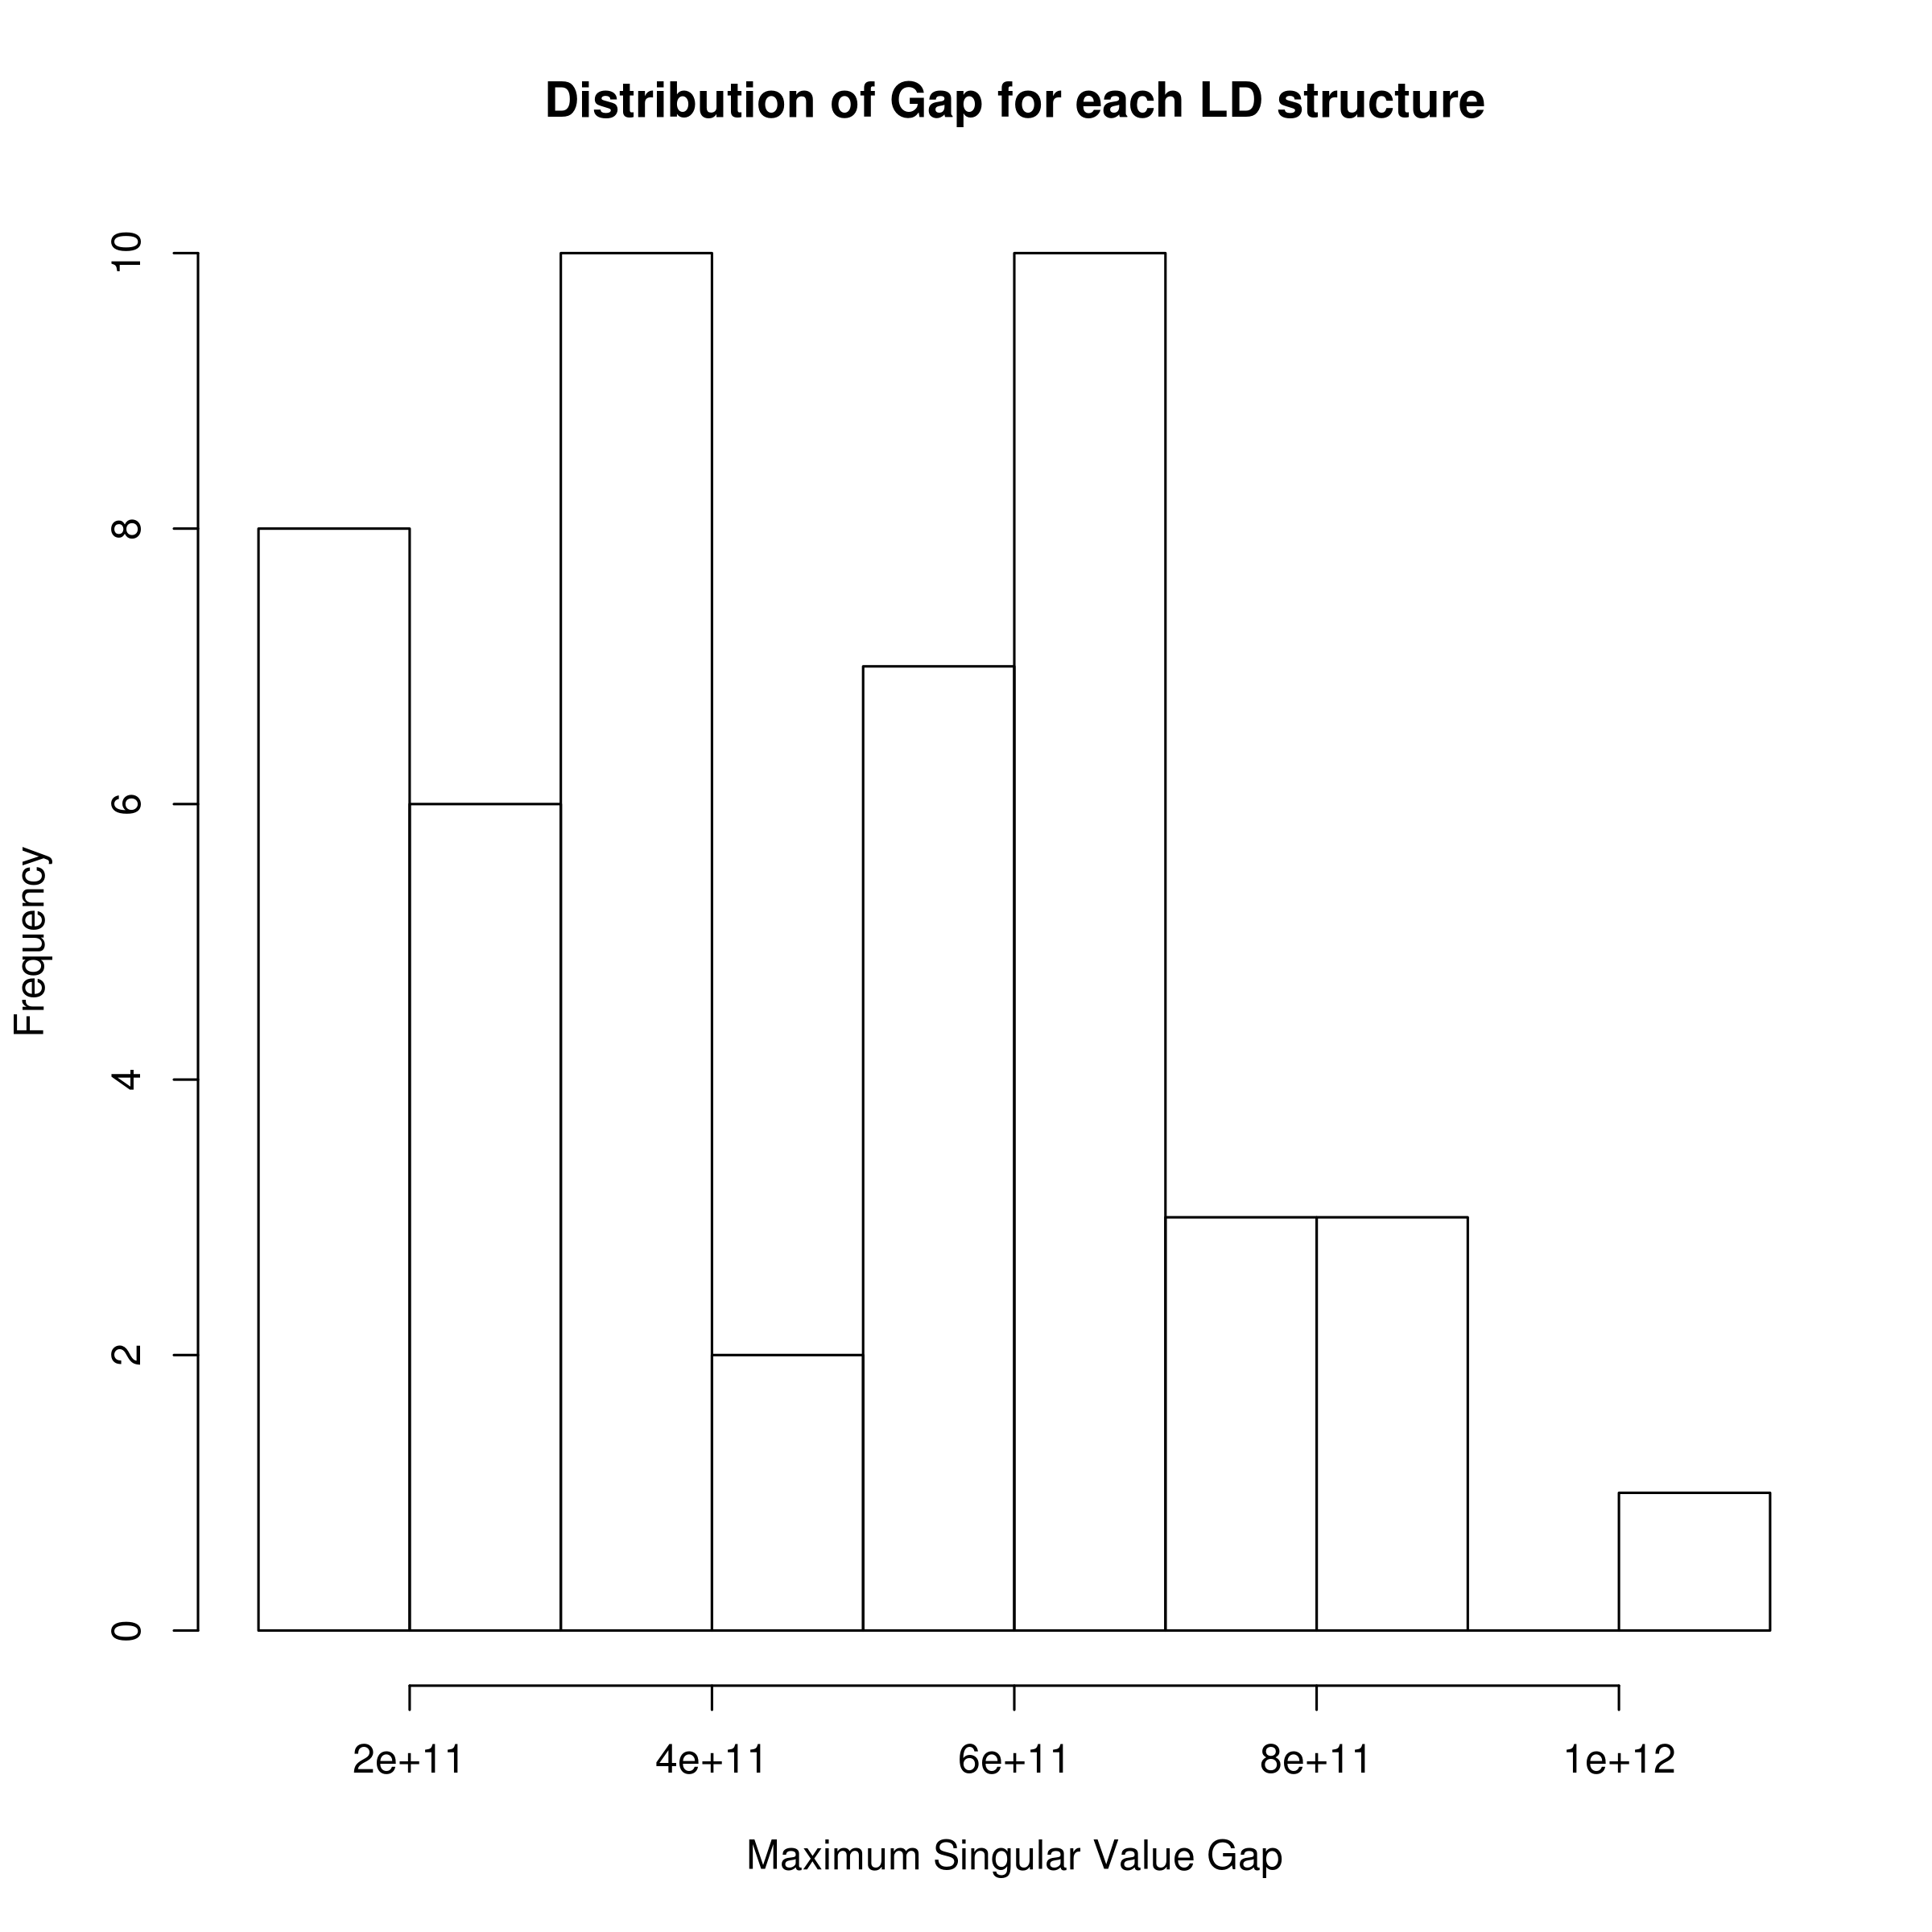
\includegraphics[width=0.5\textwidth]{figure/singular_value_distribution.png}
				\label{fig:singularValueDist}
				\vspace{-20pt}
			\end{figure}
			%\end{wrapfigure}
			
			By employing the \gls{tSVD} as a method for regularization, we were able to solve the ill-posed \cref{eq:shrekEq}, and obtain the estimated heritability.
						
		\subsection{Comparing with \glsentrylong{ldsc}}
			% main difference 
			Conceptually, the fundamental hypothesis of \gls{ldsc} and our algorithm were quite different.
			\gls{ldsc} were based on the ``global'' inflation of test statistic and its relationship to the \gls{LD} pattern.
			\gls{ldsc} hypothesize that the larger the \gls{LD} score, the more likely will the \gls{SNP} be able to ``tag'' the causal \gls{SNP} and the heritability can then be estimated through the regression between the \gls{LD} score and the test statistic.
			
			On the other hand, our algorithm focuses more on the per-\gls{SNP} level.
			Our main idea was that the individual test statistic of each \glspl{SNP} is a combination of its own effect and effect from \glspl{SNP} in \gls{LD} with it. 
			Thus, based on this concept, our algorithm aimed to ``remove'' the inflation of test statistic introduced through the \gls{LD} between \glspl{SNP} and the heritability can be calculated by adding the test statistic of all \glspl{SNP} after ``removing'' the inflation. 
			
			Mathematically, the calculation of \gls{ldsc} and our algorithm were also very different. 
			\gls{ldsc} take the sum of all $R^2$ within a 1cM region as the LD score and regress it against the test statistic to obtain the slope and intercept which represent the heritability and amount of confounding factors respectively. 
			In their model, \gls{ldsc} assume that each \glspl{SNP} will explain the same portion of heritability
			\begin{align}
			 \mathrm{Var}(\beta)&=\frac{h^2}{M}\boldsymbol{I}\\
			 M &= \text{number of SNPs}\notag\\
			 \beta &= \text{vector containing per normalized genotype effect sizes}\notag\\
			 I &= \text{identity matrix}\notag\\
			 h^2 &= \text{heritability}\notag
			\end{align}
			
			As for our algorithm, the whole \gls{LD} matrix were used and inverted to decompose the \gls{LD} from the test statistic. 
			There were no assumption of the amount of heritability explained by each \glspl{SNP}. 
			However, our algorithm does assumed that the null should be 1 and therefore cannot detect the amount of confounding factors. 
					
	\section{Simulation}
		First, we would like to test how well our algorithm works for heritability estimation under different scenarios.
		To account for different genetic architecture, we varies the heritability of the trait, the number of causal \glspl{SNP} and the genotypes(therefore varies the \gls{LD} pattern) during the quantitative trait simulation.
		
		\subsection{Sample Size}
		One important consideration in our simulation was the number of sample simulated. 
		The sample size was the most important parameter in determining the standard error of the heritability estimation. 
		As sample size increases, study will be more representative of the true population. 
		The increased number of information also means a better estimation of parameters, therefore a smaller \acrfull{se}.
		% awk -F "\t" '{print $2"\t"$9}' full | uniq | sed -e 's/[^0-9[:space:]]//g' | awk '{for(i=2;i<=NF;++i)j+=$i; print $1" "j; j=0}' | sort | uniq  %script for text mining
		Based on information from \gls{GWAS} catalog\citep{Welter2014}, we calculate the sample size distribution using simple text mining and exclude studies with conflicting sample size information in multiple entries. 
		The average sample size for all \gls{GWAS} recorded on the \gls{GWAS} catalog was 7,874, with a median count of 2,506 and a lower quartile at 940 (\cref{fig:gwasCata}). 
		We argue that if the algorithm works for studies with a small sample size (e.g lower quartile sample size), then it should perform even better when the sample size is larger. 
		Thus, we only simulate 1,000 samples in our simulation, which roughly represent the lower quartile sample size range.
		
		\begin{wrapfigure}{R}{8cm}
			\centering
			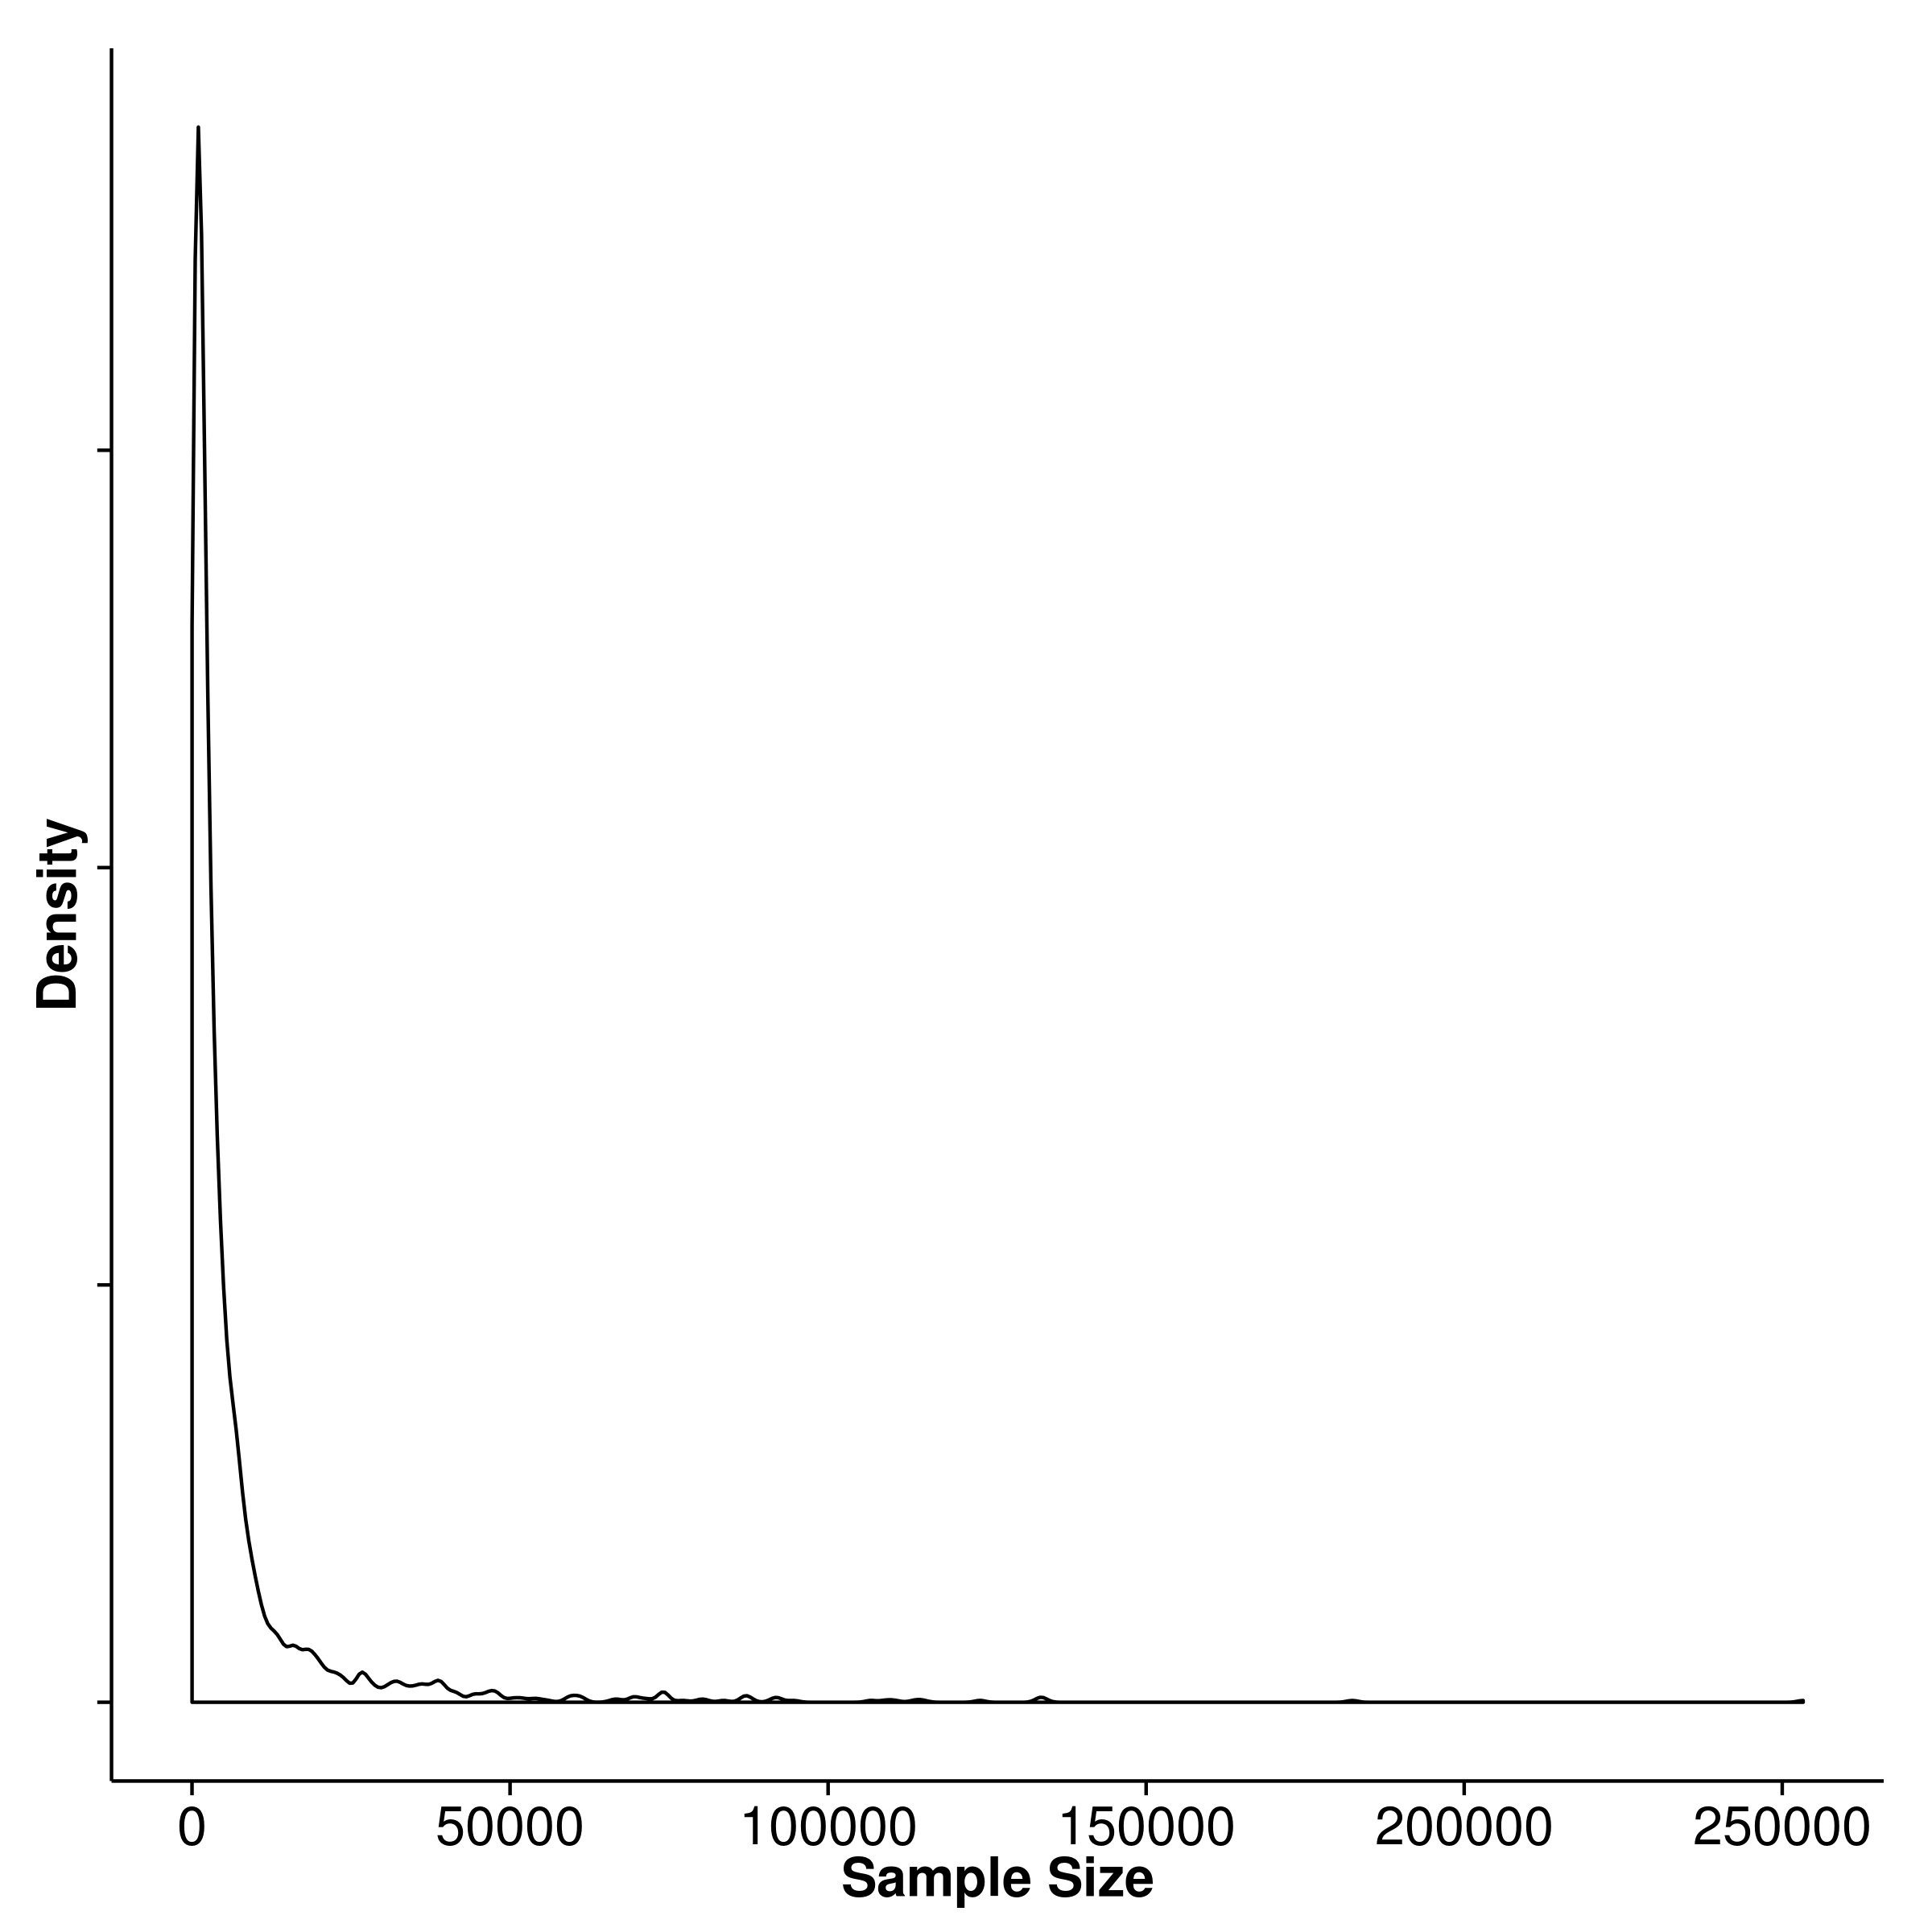
\includegraphics[width=0.5\textwidth]{figure/gwasSampleSize.png}
			\caption[GWAS Sample Size distribution]{
				\gls{GWAS} sample size distribution.
				}
			\label{fig:gwasCata}
		\end{wrapfigure}
		
		\subsection{Number of SNPs in Simulation}
		Another consideration in the simulation was the number of \glspl{SNP} included.
		In a typical \gls{GWAS} study, there are usually a larger number of \glspl{SNP} when compared to the sample size. 
		Fr example, in the \gls{pgc} \glng{scz} \gls{GWAS}, more than 9 million \glspl{SNP} were included, with around 700,000 \glspl{SNP} on chromosome 1.
		Although it would be idea to simulate 700,000 \glspl{SNP} in our simulation, the time required for simulating the samples will become unrealistic.
		
		As the number of \glspl{SNP} simulated grow, more time were required for the simulation of samples and more calculation will be required.
		Moreover, the increasing number of \glspl{SNP} will lead to increased size of the \gls{LD} matrix, requiring a long time for the inverse of the matrix.
		In reality, this should not be a real problem as one typically only calculate the heritability of the data set once and the speed of the algorithm is still relatively fast. 
		However, in the case of simulation where we would like to repeat the same analysis many times, the small increment of time will lead to an escalation in total simulation time, making the simulation infeasible. 
		To compromise, we simulate a total of 50,000 \glspl{SNP} from chromosome 1 as a balance between run time of simulation and the total \glspl{SNP} simulated.
		
		\subsection{Genetic Architecture}
		Of all simulation parameter, the genetic architecture was the most complicated and important parameter. 
		The \gls{LD} pattern, the number of causal \glspl{SNP}, the effect size of the causal \glspl{SNP} and the heritability of the trait were all important factors contribute to the genetic architecture of a trait. 
		
		First and foremost, because the aim of the algorithm was to estimating the heritability of the trait, it is important that the algorithm works for traits from different heritability spectrum.
		We therefore simulate traits with heritability ranging from 0 to 0.9, with increment of 0.1.
		
		Secondly, in real life scenario, the ``causal'' variant might not be readily included on the \gls{GWAS} chip and were only ``tagged'' by \glspl{SNP} included on the \gls{GWAS} chip.
		However, to simplify our simulation, all ``causal'' variants were included in our simulation (e.g. perfectly ``tagged'')
		
		Thirdly, to obtain a realistic \gls{LD} pattern, we simulate the genotypes using the HAPGEN2 programme\citep{Su2011}, using the 1000 genome \gls{CEU} haplotypes as an input.
		In short, HAPGEN2 simulate new haplotypes as an imperfect mosaic of haplotpyes from a reference panel and the haplotypes that have already been simulated using the \textit{Li and Stephens} (LS) model of \gls{LD} \citep{Li2003}.
		In a typical \gls{GWAS} , one usually only have power in detecting ``common variants'', usually defined as variants with \gls{maf} $\ge 0.01$.
		We therefore only consider scenario with ``common'' variants and only use \glspl{SNP} with \gls{maf} $\ge0.1$ in the \gls{CEU} haplotypes as an input to HAPGEN2. 
		This will reduce the probability of having \glspl{SNP} with \gls{maf} $<0.01$ in the final simulated sample sets.
		
		Finally, we would like to simulate traits with different inheritance model such as oligogenic traits and polygenic traits.
		We therefore varies the number of causal \glspl{SNP} ($k$) with $k\in\{5, 10, 50, 100, 250, 500\}$.
		
		
		To assess how well our algorithm performs for narrow sense heritability estimation in comparison to other current methods, we performed series of systematic simulation.
		In these simulations, performance of our algorithm, \gls{gcta} \citep{Yang2011} and \gls{ldsc} \citep{Bulik-Sullivan2015} with and without the intercept estimation function (-{}-no-intercept) were tested.
		Through simulation, we can obtain the sample distribution of the heritability estimate under different study designs (e.g. Quantitativat traits, Case-Control studies or extreme phenotype selection). 
		Factors considered in our simulations were as follow:		
		
		
		
		\subsection{Genetic Architecture} % Should contain the effect size distribution, the causal SNP number and the heritability spectrum
		Of all the simulation parameter, the genetic architecture was arguably the most complicated parameter. 
		It involves the \gls{LD} pattern, the distribution of effect size, the number of causal \glspl{SNP}, the \gls{maf} of the causal \glspl{SNP} and most importantly, the heritability of the trait ($h^2$).
		
		Because we would like to cover most of the heritability spectrum, we will simulate traits with $h^2$ ranging from 0 to 0.9, with increment of 0.1 such that $h^2 \in \{0,\allowbreak 0.1,\allowbreak 0.2,\allowbreak 0.3,\allowbreak 0.4,\allowbreak 0.5,\allowbreak 0.6,\allowbreak 0.7,\allowbreak 0.8,\allowbreak 0.9\}$.
		To simplify the condition, all ``causal'' variants were included in the simulation (e.g. perfect tagging).
		We also try to obtain realistic \gls{LD} pattern by using HAPGEN2\citep{Su2011} to simulate genotype based on the \gls{LD} pattern of the 1000 genome \gls{CEU} samples. 
		
		
		First, we only consider situation of common \glspl{SNP} and only simulate \glspl{SNP} with \gls{maf} $> 0.1$.
		In these simulation, we varies the number of causal \glspl{SNP} ($k$) and the effect size distribution.
		We consider $k\in\{5, 10, 50, 100, 250, 500\}$ such that we can cover different disease spectrum (Oligogenic to Polygenic diseases). 
		As for effect size distribution, we considered two conditions:
		\begin{enumerate}
			\item Equal Effect Size
			\item Random Effect Size
		\end{enumerate}
		The simplest situation was when all casual \glspl{SNP} have the same effect size 
		\begin{equation}
		\beta_s=\pm\sqrt{\frac{h^2}{k}}
		\label{eq:stableEffect}
		\end{equation}
		The direction of effect should be randomly simulated.
		As for the random effect size scenario, we consider the effect size to be 
		\begin{equation}
		\beta_r=\pm\sqrt{\frac{\gamma \times h^2}{\sum \gamma}}
		\label{eq:randomEffect}
		\end{equation}
		with $\gamma\sim exp(\lambda=1)$ and a random direction of effect.
		Rationale behind the choice of exponential distribution was based on \citet{Orr1998}, which suggested that exponential distribution with $\lambda=1$ may serve as a heuristic expectation the genetic architecture of adaptation.

		Once the effect size was calculated, we can then randomly assign the effect size to $k$ random \glspl{SNP} with normalized genotype $\boldsymbol{X}$, the phenotype can then be calculated as 
		\begin{align}
		\epsilon_i&\sim N(0,\sqrt{\mathrm{Var}(\boldsymbol{X\beta})\frac{1-h^2}{h^2}} )\notag\\
		\boldsymbol{\epsilon} &= (\epsilon_1,\epsilon_2,...,\epsilon_n)^t\notag\\
		\boldsymbol{y} &= \boldsymbol{X\beta}+\boldsymbol{\epsilon}
		\label{eq:simulationOfPhenotype}
		\end{align}
		
		For each batch of simulated samples, we calculate the estimated heritability using our algorithm, \gls{gcta}, \gls{ldsc} with intercept fixed at 1 and \gls{ldsc} allowing for intercept estimation for each $h^2$.
		In each iteration, the sample genotype was provided to \gls{gcta} for the calculation of genetic relationship matrix (GRM) whereas for our algorithm and \gls{ldsc}, 500 independent samples were simulated based on the 1000 genome project \gls{CEU} samples\parencite{Project2012} to construct the \gls{LD} matrix and calculate the \gls{LD} score respectively.
		This was because both \gls{ldsc} and our algorithm were designed to work in situation where the raw genotype were not provided and the \gls{LD} structure was usually obtained form the public data base instead.
		Therefore to provide a realistic simulation, an independent set of reference samples were provided for our algorithm and \gls{ldsc}.
		
		The whole process were repeated 50 times with the same \glspl{SNP} set, the same causal \glspl{SNP} and the same effect size for each $h^2$ such than an empirical variance can be obtained.
		We then repeat the process 10 times on different \glspl{SNP} sets, with different causal \glspl{SNP} but the same effect size for each $h^2$.
		This should introduce a slight variation in the \gls{LD} structure and should demonstrate the robustness of the programmes under different \gls{LD} construct.
		To summarize, the simulation procedure follows:
		\begin{enumerate}
			\item Randomly select 50,000 \glspl{SNP} with \gls{maf}$>0.1$ from chromosome 1
			\item Randomly generate $k$ effect size with $k \in \{5,10,50,100,250,500\}$ following either \cref{eq:stableEffect} or \cref{eq:randomEffect}
			\item Randomly assign the effect size to $k$ \glspl{SNP}
			\item Simulate 1,000 samples using HAPGEN2 and calculate their phenotype according to \cref{eq:simulationOfPhenotype}
			\item Perform heritability estimation using our algorithm, \gls{ldsc} and \gls{gcta}
			\item Repeat step 4-5 50 times
			\item Repeat step 1-6 10 times
		\end{enumerate}
		
		\subsubsection{Extreme Effect Size}
		Another condition we were interested in was the performance of the tools when there is a small amount of \glspl{SNP} that explain a large portion of effect e.g. 50\%.
		Similarly, we only consider 1,000 samples, with 50,000 common \glspl{SNP}(\gls{maf} $>0.1$).
		We hypothesize that under the polygenic model, such extreme distribution in effect size should have much larger effect when compared to that in oligogenic condition. 
		Thus we only consider the polygenic condition where the number of causal \gls{SNP} ($k$) were limited to 100 or 250. 
		
		We simulate $m$ \glspl{SNP} accounting for 50\% of all the effect where $m\in\{1,5,10\}$.
		The effect size was then calculated as
		\begin{align}
		\beta_{eL} &= \pm\sqrt{\frac{0.5h^2}{m}} \notag\\
		\beta_{eS} &= \pm\sqrt{\frac{0.5h^2}{k-m}} \notag\\
		\beta &= \{\beta_{eL}, \beta_{eS}\}
		\label{eq:extremEffect}
		\end{align}
		the effect size were then randomly assigned to $k$ causal \glspl{SNP} and phenotype was calculated as in \cref{eq:simulationOfPhenotype}.
		The simulation procedure then becomes
		\begin{enumerate}
			\item Randomly select 50,000 \glspl{SNP} with \gls{maf}$>0.1$ from chromosome 1
			\item Randomly generate $k$ effect size with $k \in \{100,250\}$ and $m$ extreme effect, following \cref{eq:extremEffect} where $m\in{1,5,10}$
			\item Randomly assign the effect size to $k$ \glspl{SNP}
			\item Simulate 1,000 samples using HAPGEN2 and calculate their phenotype according to \cref{eq:simulationOfPhenotype}
			\item Perform heritability estimation using our algorithm, \gls{ldsc} and \gls{gcta}
			\item Repeat step 4-5 50 times
			\item Repeat step 1-6 10 times
		\end{enumerate}
		
		\subsection{Case Control Studies}
		The simulation of case control studies was very much like that of the simulation of quantitative trait. 
		However, there were two additional parameters to consider: the population prevalence and the observed prevalence.
		These parameters allow us to simulate the samples under a liability model, therefore simulating the case control studies.

		Although there were only two additional parameter, the computational challenge for the simulation of case control was significantly bigger than that for the simulation of quantitative trait.
		Take for example, if one like to simulate a trait with population prevalence of $p$ and observed prevalence  of $q$ and would like to have $n$ cases in total, one will have to simulate $\min(\frac{n}{p}, \frac{n}{q})$ samples.
		Considering the scenario where the observed prevalence is 50\%, the population prevalence is 1\% and 1,000 cases,a minimum of 100,000 samples will be required.
		
		% Maybe instead of chromosome 1, use chromosome 22 and reduce the number of SNPs, that will be better.
		Given limited computer resources, we only simulate 1,000 cases, with an observed prevalence of 0.5 and population prevalence $p\in\{0.5, 0.1, 0.05, 0.01\}$.
		Most importantly, we reduce the number of \glspl{SNP} simulated to 5,000 and used chromosome 22 instead, such that the \glspl{SNP} density remains more or less unchanged by the number of processes required were largely reduced.
		We acknowledged that the current simulation was relatively brief, however, it should be able to serve as a prove of concept simulation to study the performance of the tools under the case control scenario.
		
		\subsection{Extreme Phenotype Selection}
		The simulation of extreme phenotype selection was the same as the quantitative trait simulation. 
		The only difference being that instead of using all samples for heritability estimation, we only use the extreme 10\% of samples among the population for the heritability estimation.
		In brief, instead of simulating 1,000 samples, we simulate 5,000 samples following the exact procedure in the quantitative trait simulation with random effect size.
		However, after simulation of the phenotype using \cref{eq:simulationOfPhenotype}, we standardize the phenotype and only select the top 10\% and bottom 10\% samples (500 samples each) from the sample distribution.
		We then perform the same simulation procedure as in the quantitative trait simulation with random effect size.
		
		It was noted that the extreme phenotype selection were not supported by the \gls{ldsc} and \gls{gcta}.
		To allow comparison in such scenario, we apply the extreme phenotype adjustment from \citet{Sham2014} to the estimation obtained from \gls{ldsc} and \gls{gcta}.
		
	\section{Result}
		The heritabilibty estimation were implemented in \gls{shrek} and is available on \url{https://github.com/choishingwan/shrek}.  
		
		To study the performance of \gls{shrek} and \gls{ldsc} in comparison to \gls{gcta}, we performed a variety of simulations to model scenarios with different number of causal \glspl{SNP}, different effect size distribution and different type of traits. 
		
		First, we examined the performance of the programmes under the quantitative trait scenario. 
		In the quantitative trait scenario, we varies the number of causal \glspl{SNP} and either assigned an equal effect size to each causal \glspl{SNP} or assigned a per-allele effect sizes drawn from the squared root of the exponential distribution with $\lambda=1$.
		
		\subsection{Quantitative Trait Simulation with Equal Effect Size}
		% QT Equal Effect
		
		\begin{figure}
			\centering
			\subfloat[SHREK]{
				\scalebox{.4}{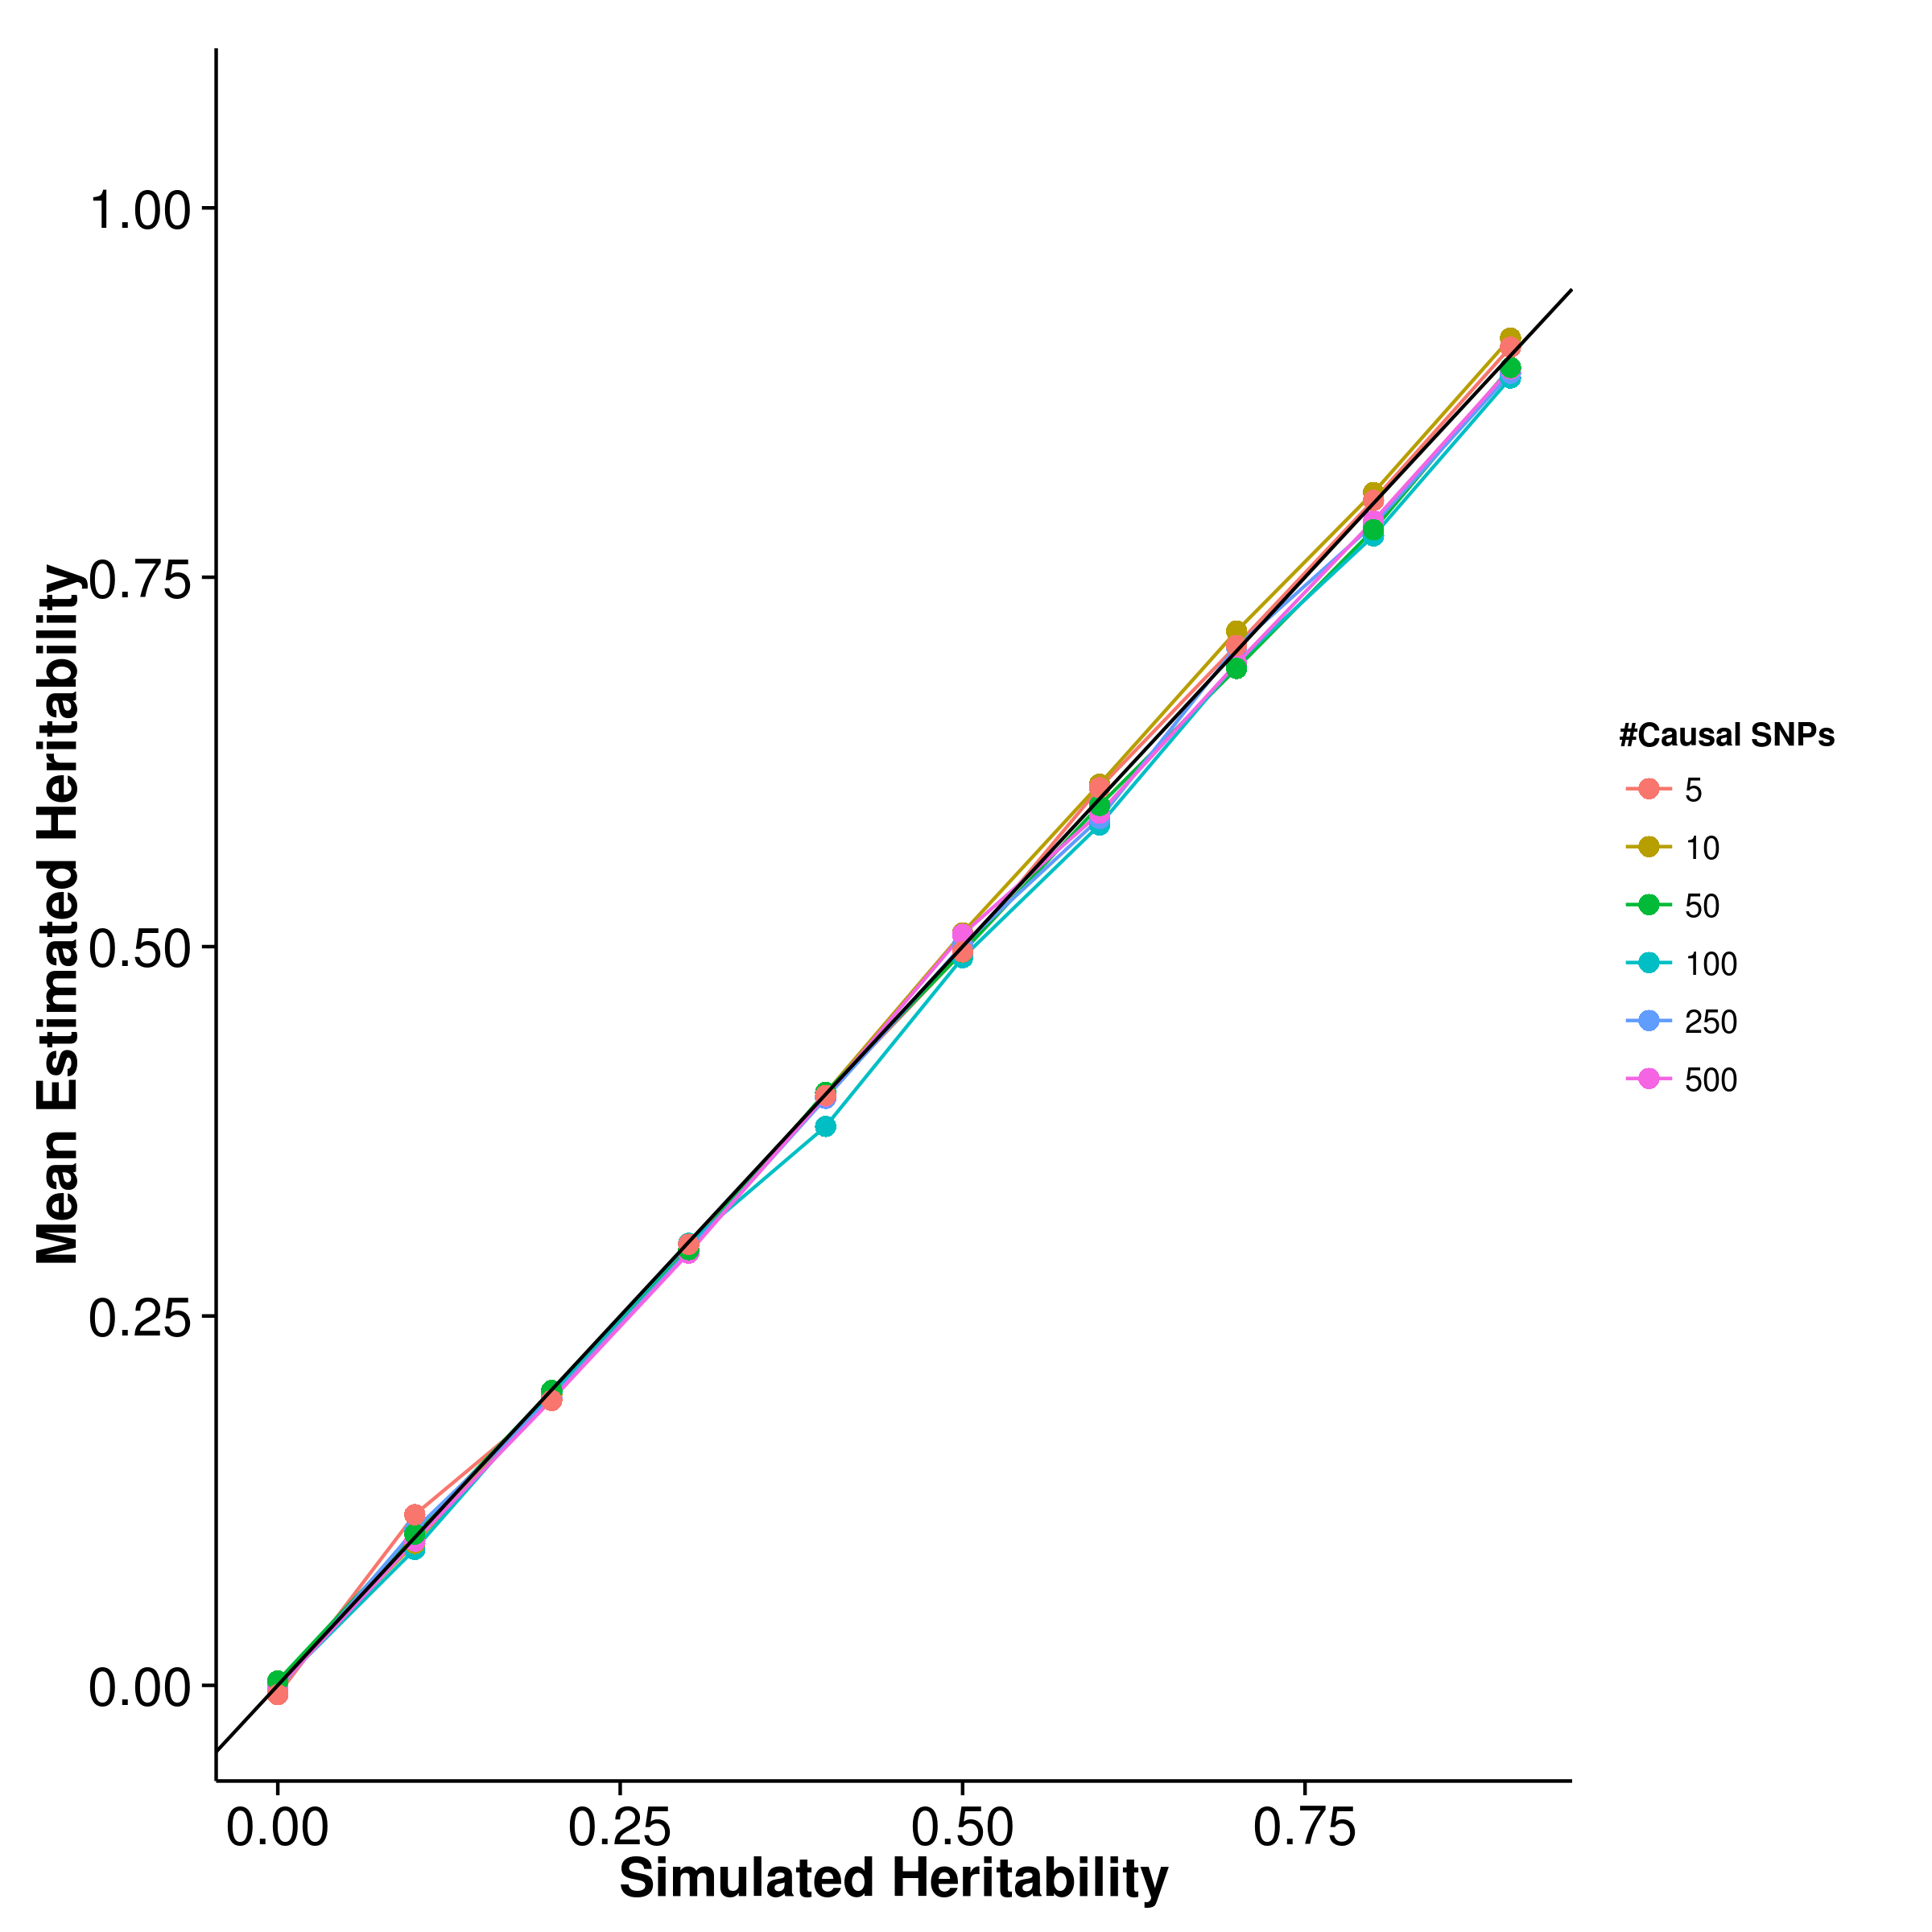
\includegraphics{figure/he_summary/equal/shrek_Qt_Equal_mean.png}}
				\label{fig:shrekQtEqualMean}
			}
			\subfloat[GCTA]{
				\scalebox{.4}{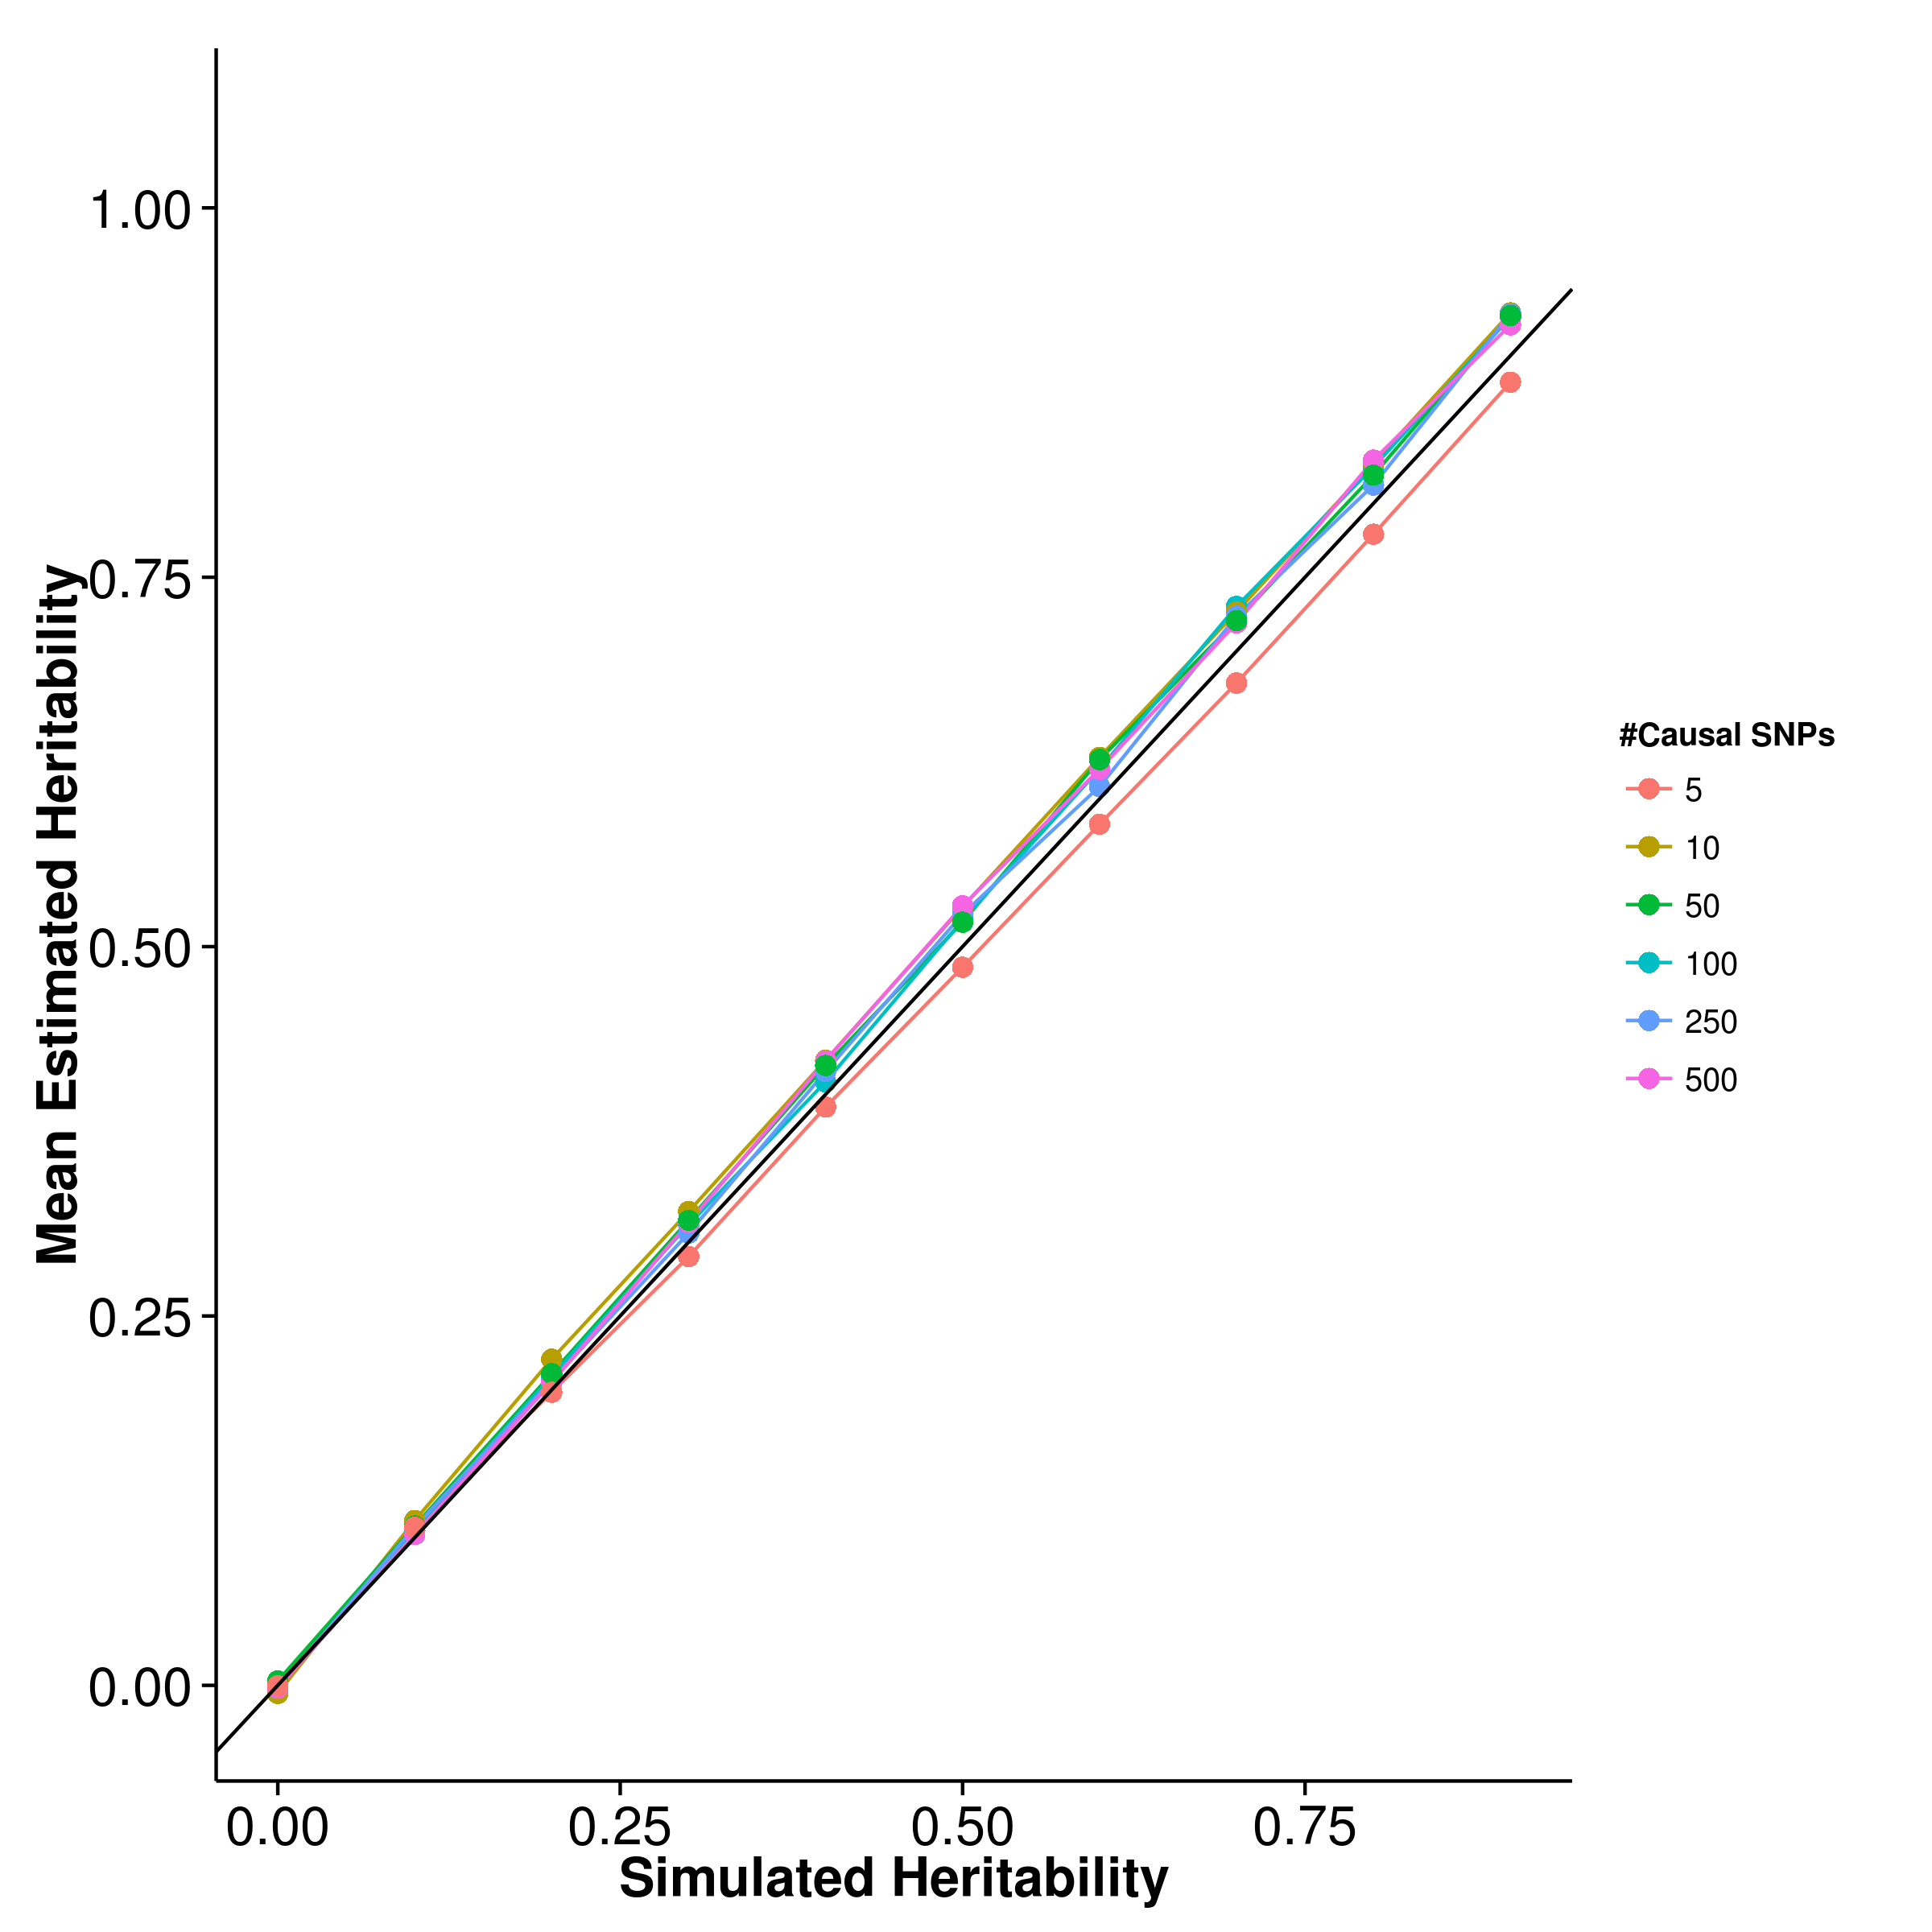
\includegraphics{figure/he_summary/equal/gcta_Qt_Equal_mean.png}}
				\label{fig:gctaQtEqualMean}
			}\\
			\subfloat[LDSC with fix intercept]{
				\scalebox{.4}{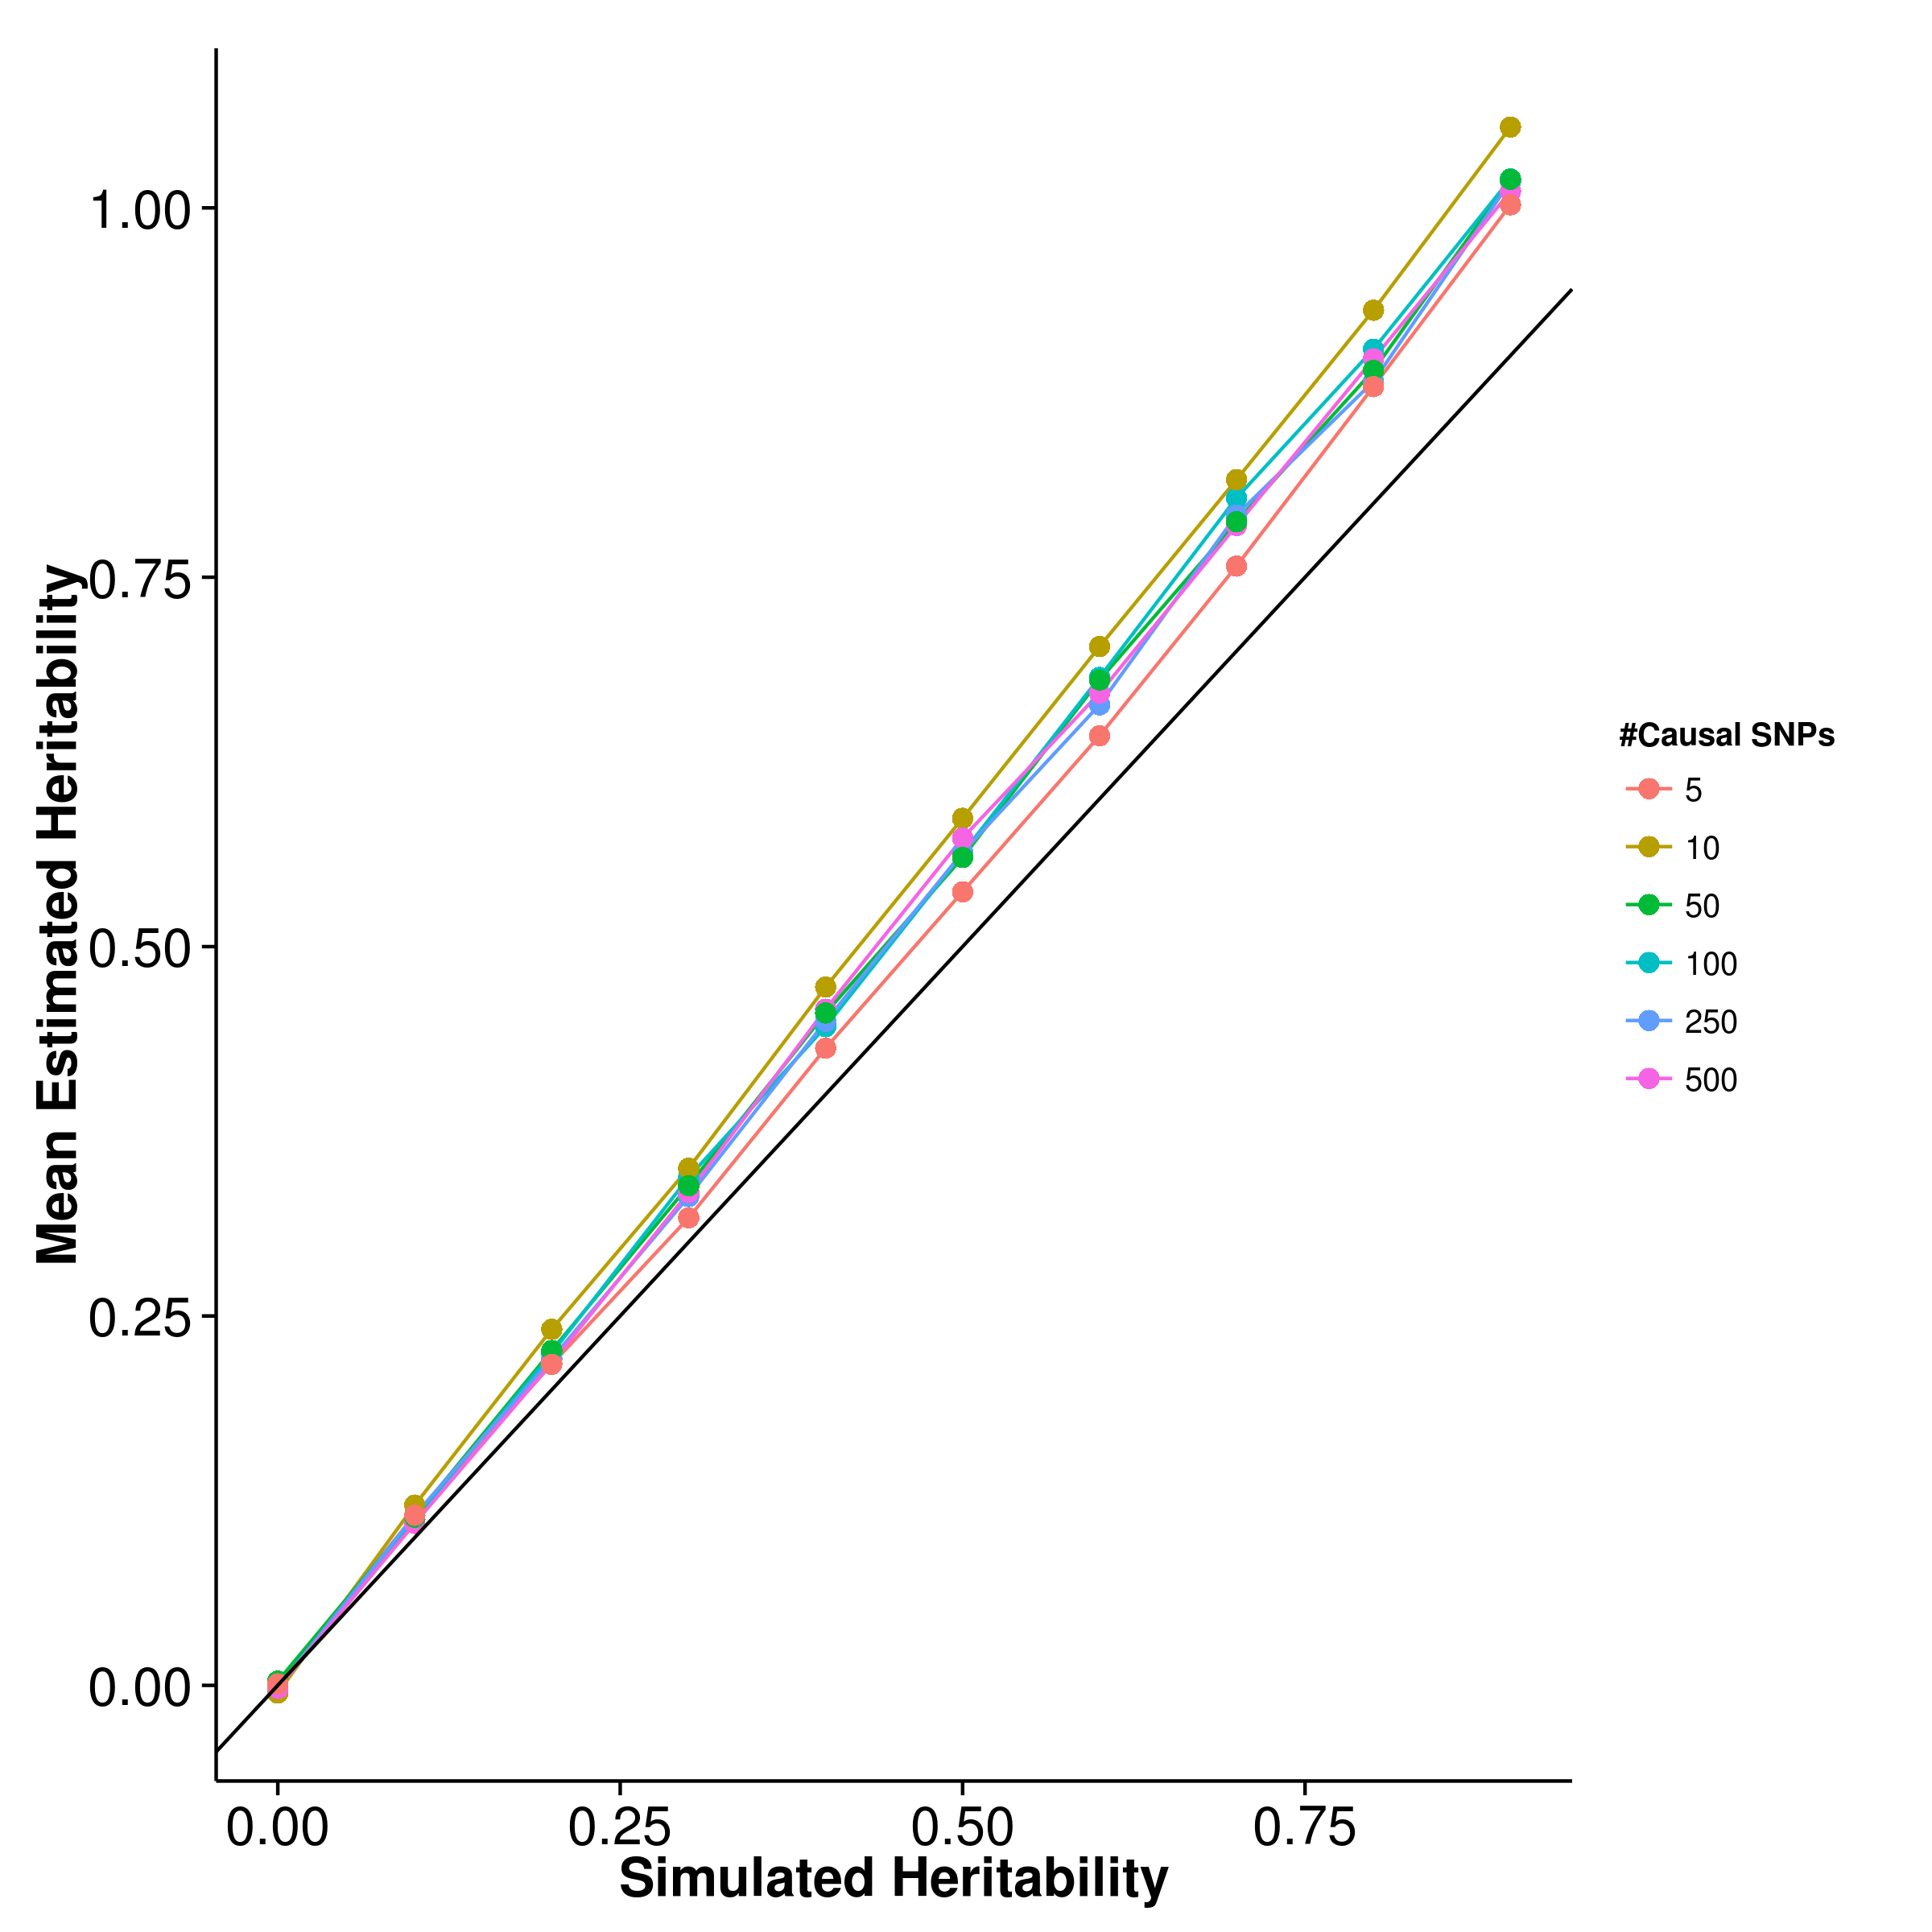
\includegraphics{figure/he_summary/equal/ldsc_Qt_Equal_mean.png}}
				\label{fig:ldscQtEqualMean}
			}
			\subfloat[LDSC with intercept estimation]{
				
				\scalebox{.4}{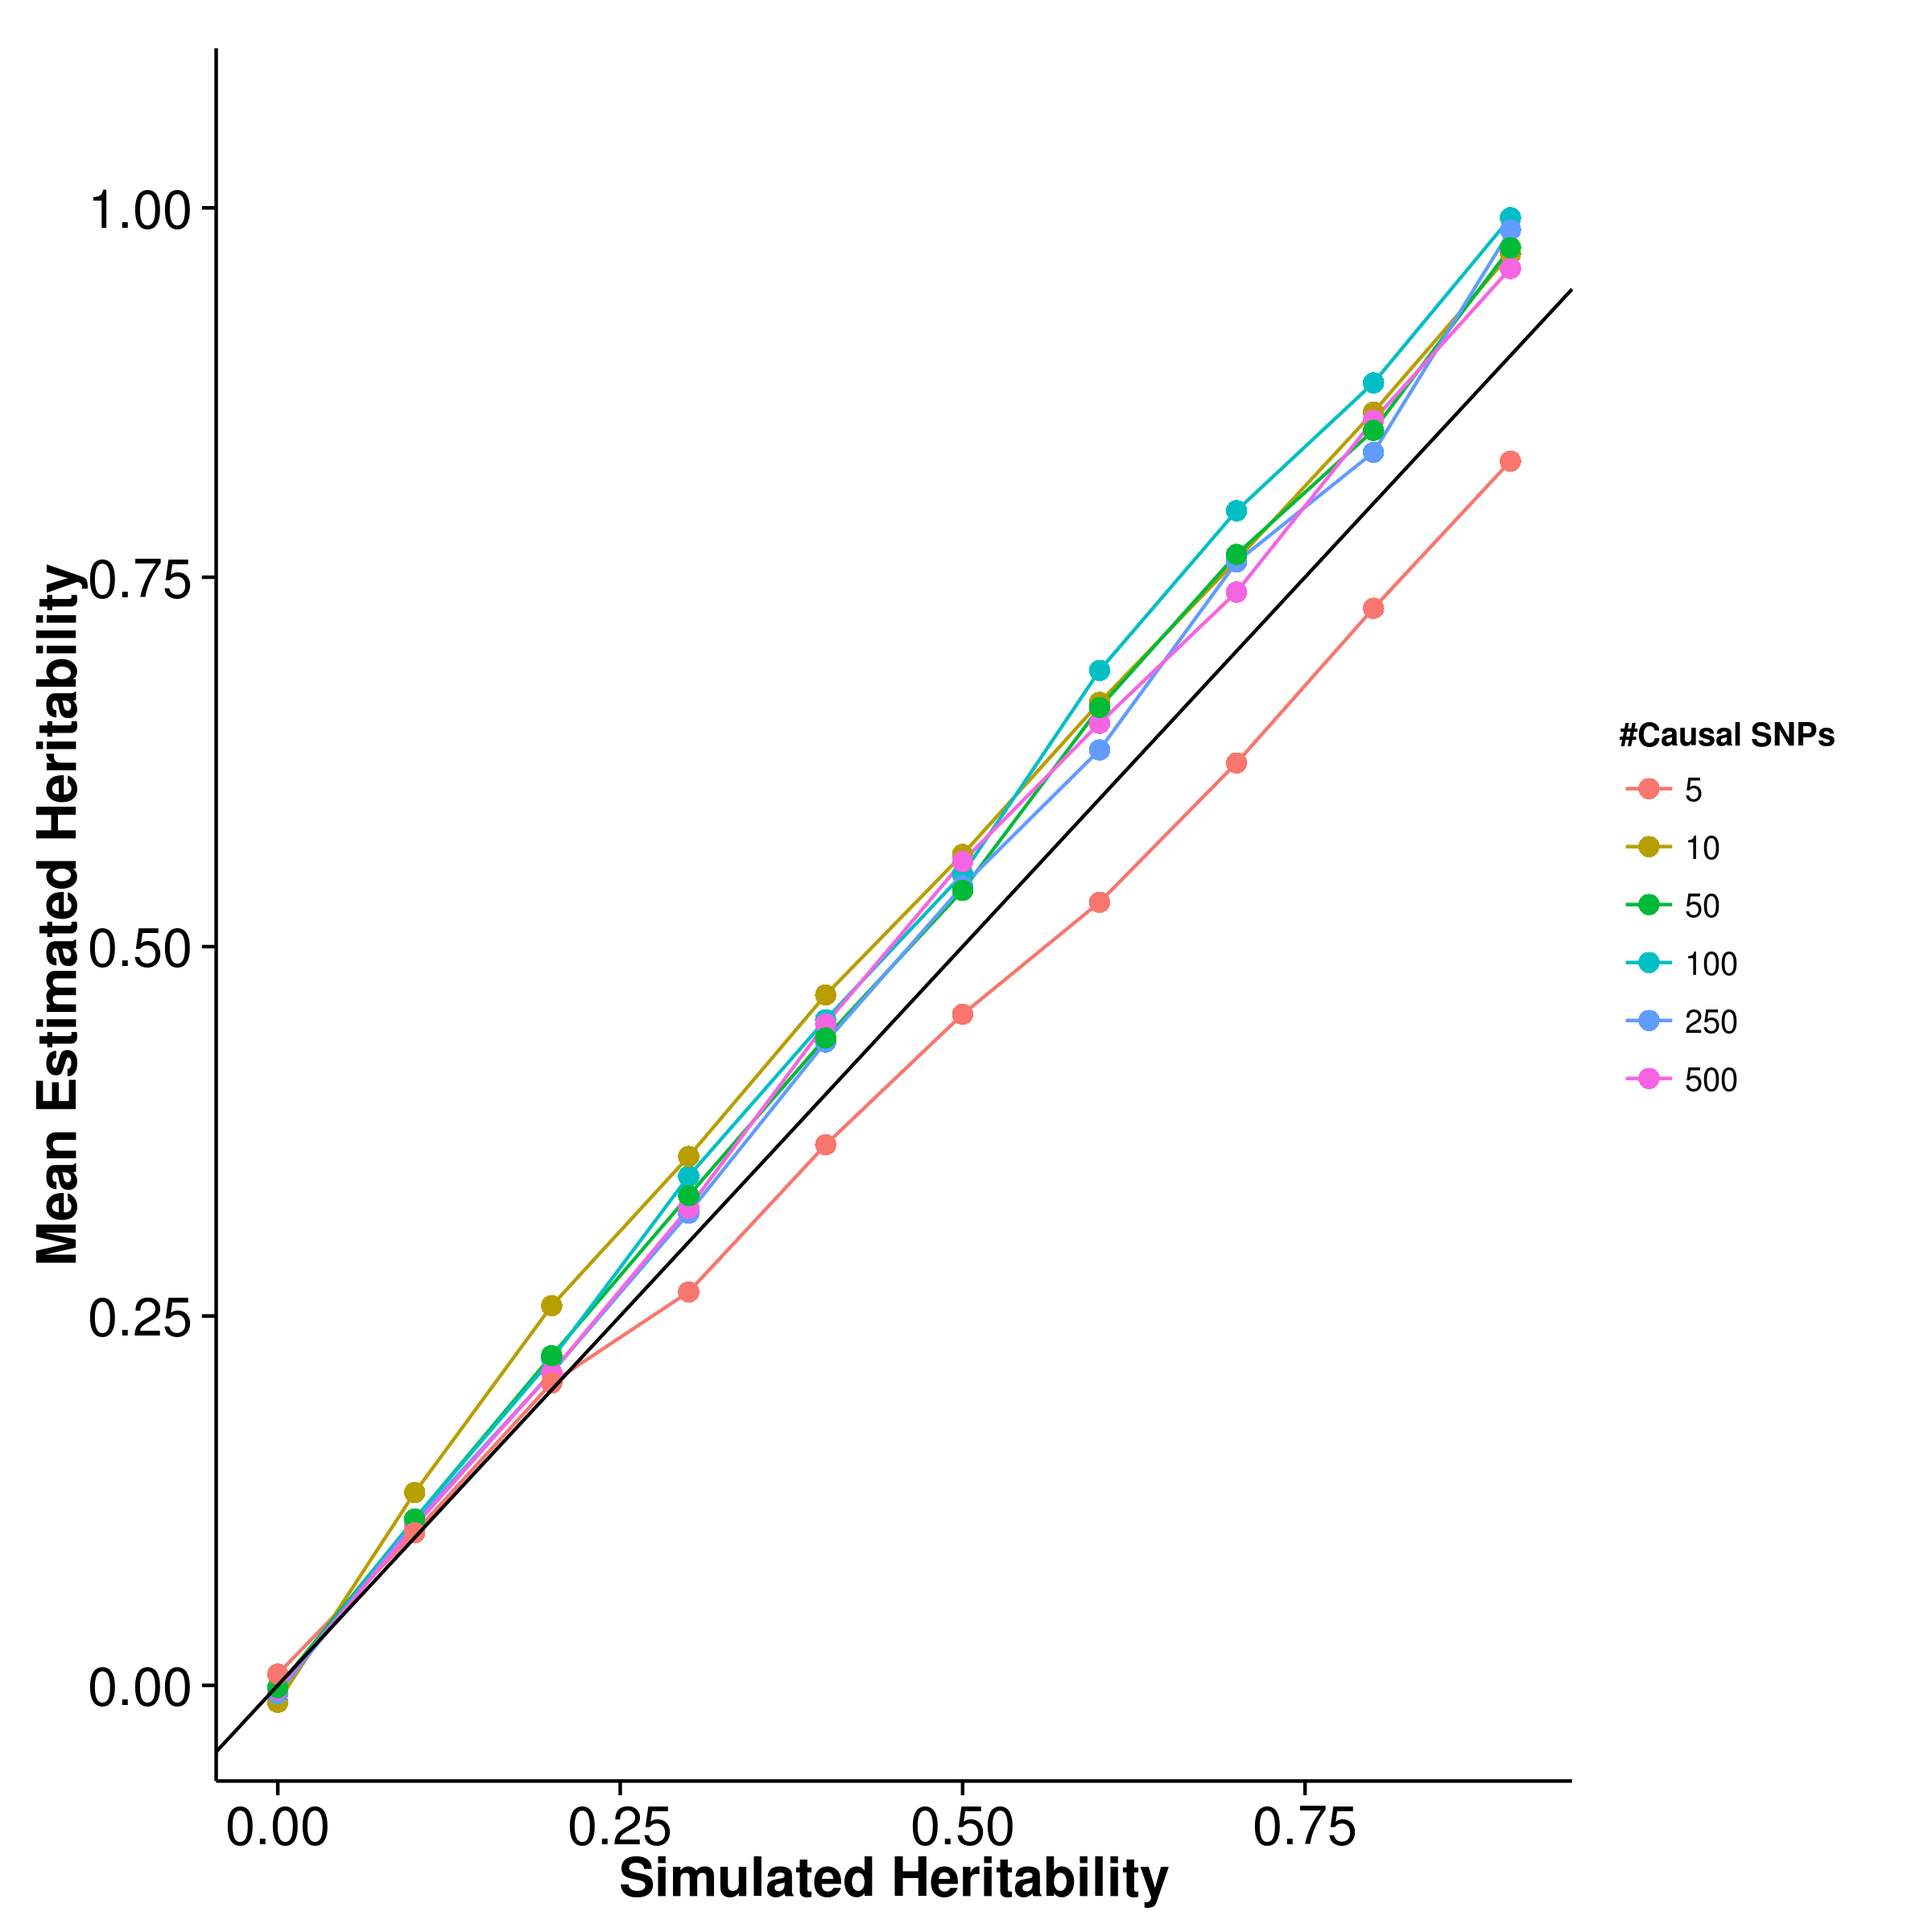
\includegraphics{figure/he_summary/equal/ldscIn_Qt_Equal_mean.png}}
				\label{fig:ldscInQtEqualMean}
			}
			\caption[Quantitative Trait with Equal Effect Size Simulation Result(Mean)]
			{Mean of results from quantitative trait simulation with equal effect size simulation.
				\gls{shrek} was found to be less biased of all the tools whereas there was a slight upward bias for \gls{ldsc} when the intercept was fixed, especially when the number of causal \glspl{SNP} was small.} 
			\label{fig:QtEqualMean}
		\end{figure}
		
		\begin{figure}
			\centering
			\subfloat[SHREK]{
				\scalebox{.4}{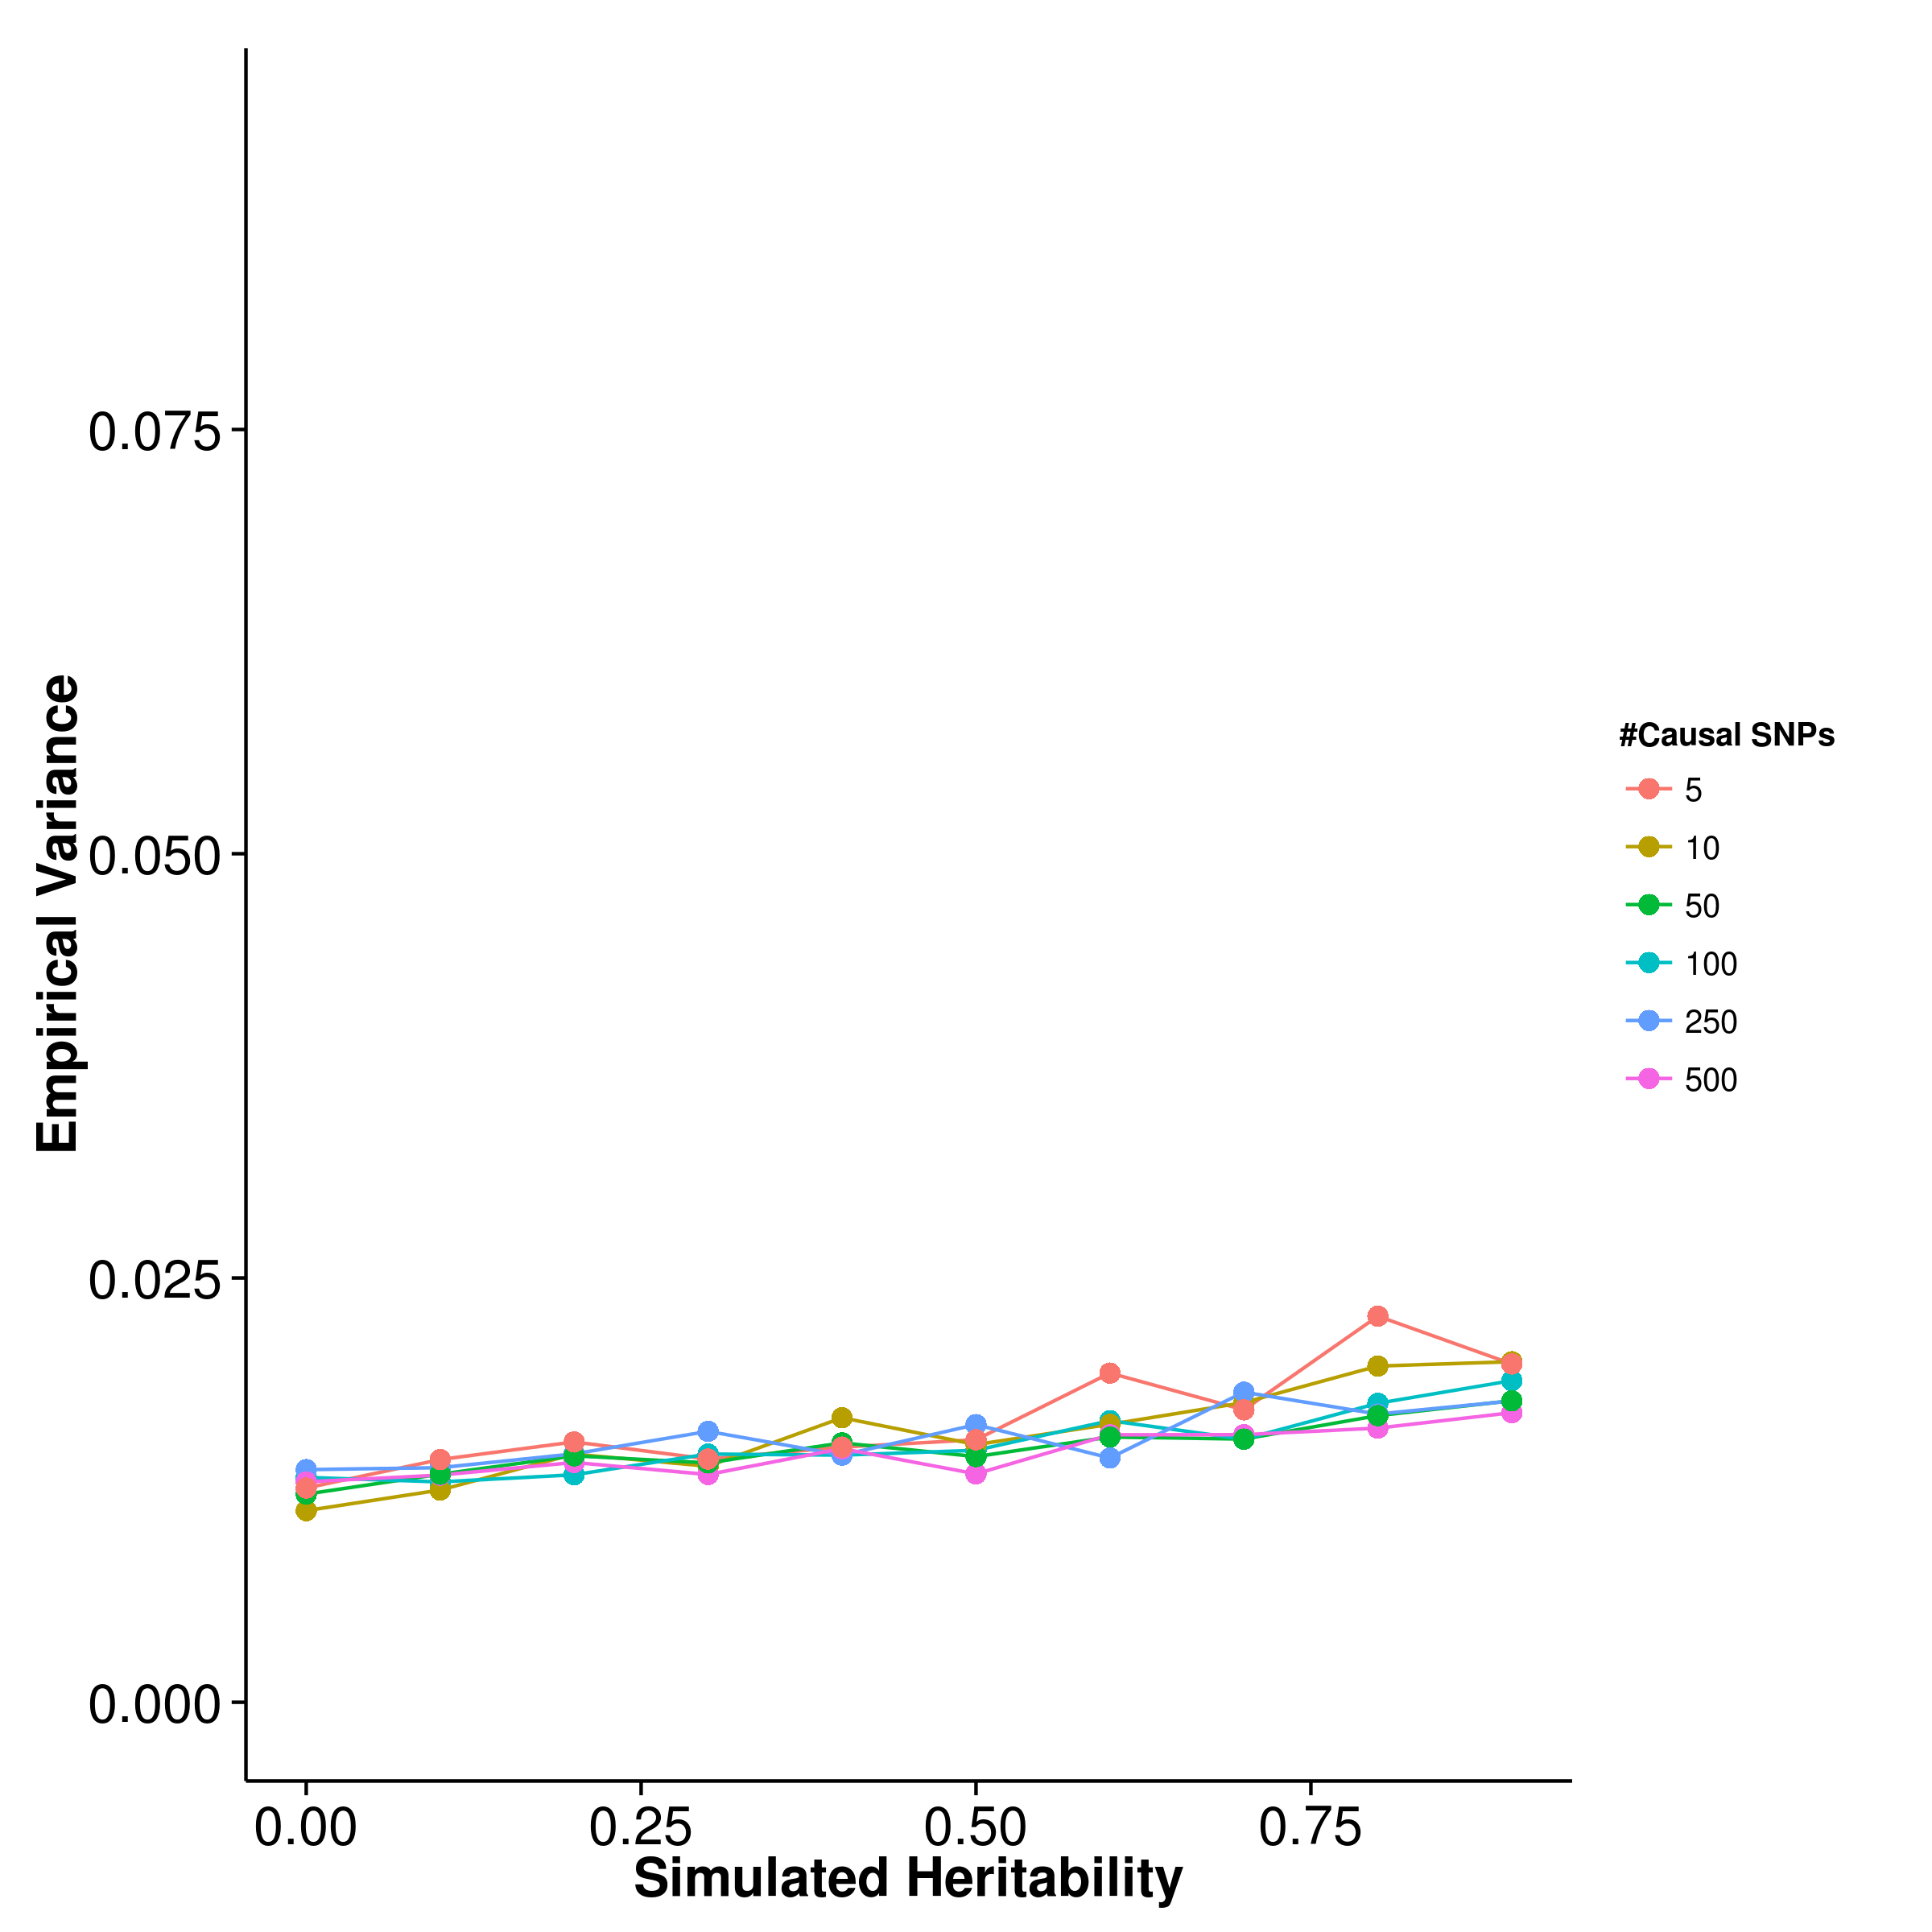
\includegraphics{figure/he_summary/equal/shrek_Qt_Equal_sd.png}}
				\label{fig:shrekQtEqualVar}
			}
			\subfloat[GCTA]{
				\scalebox{.4}{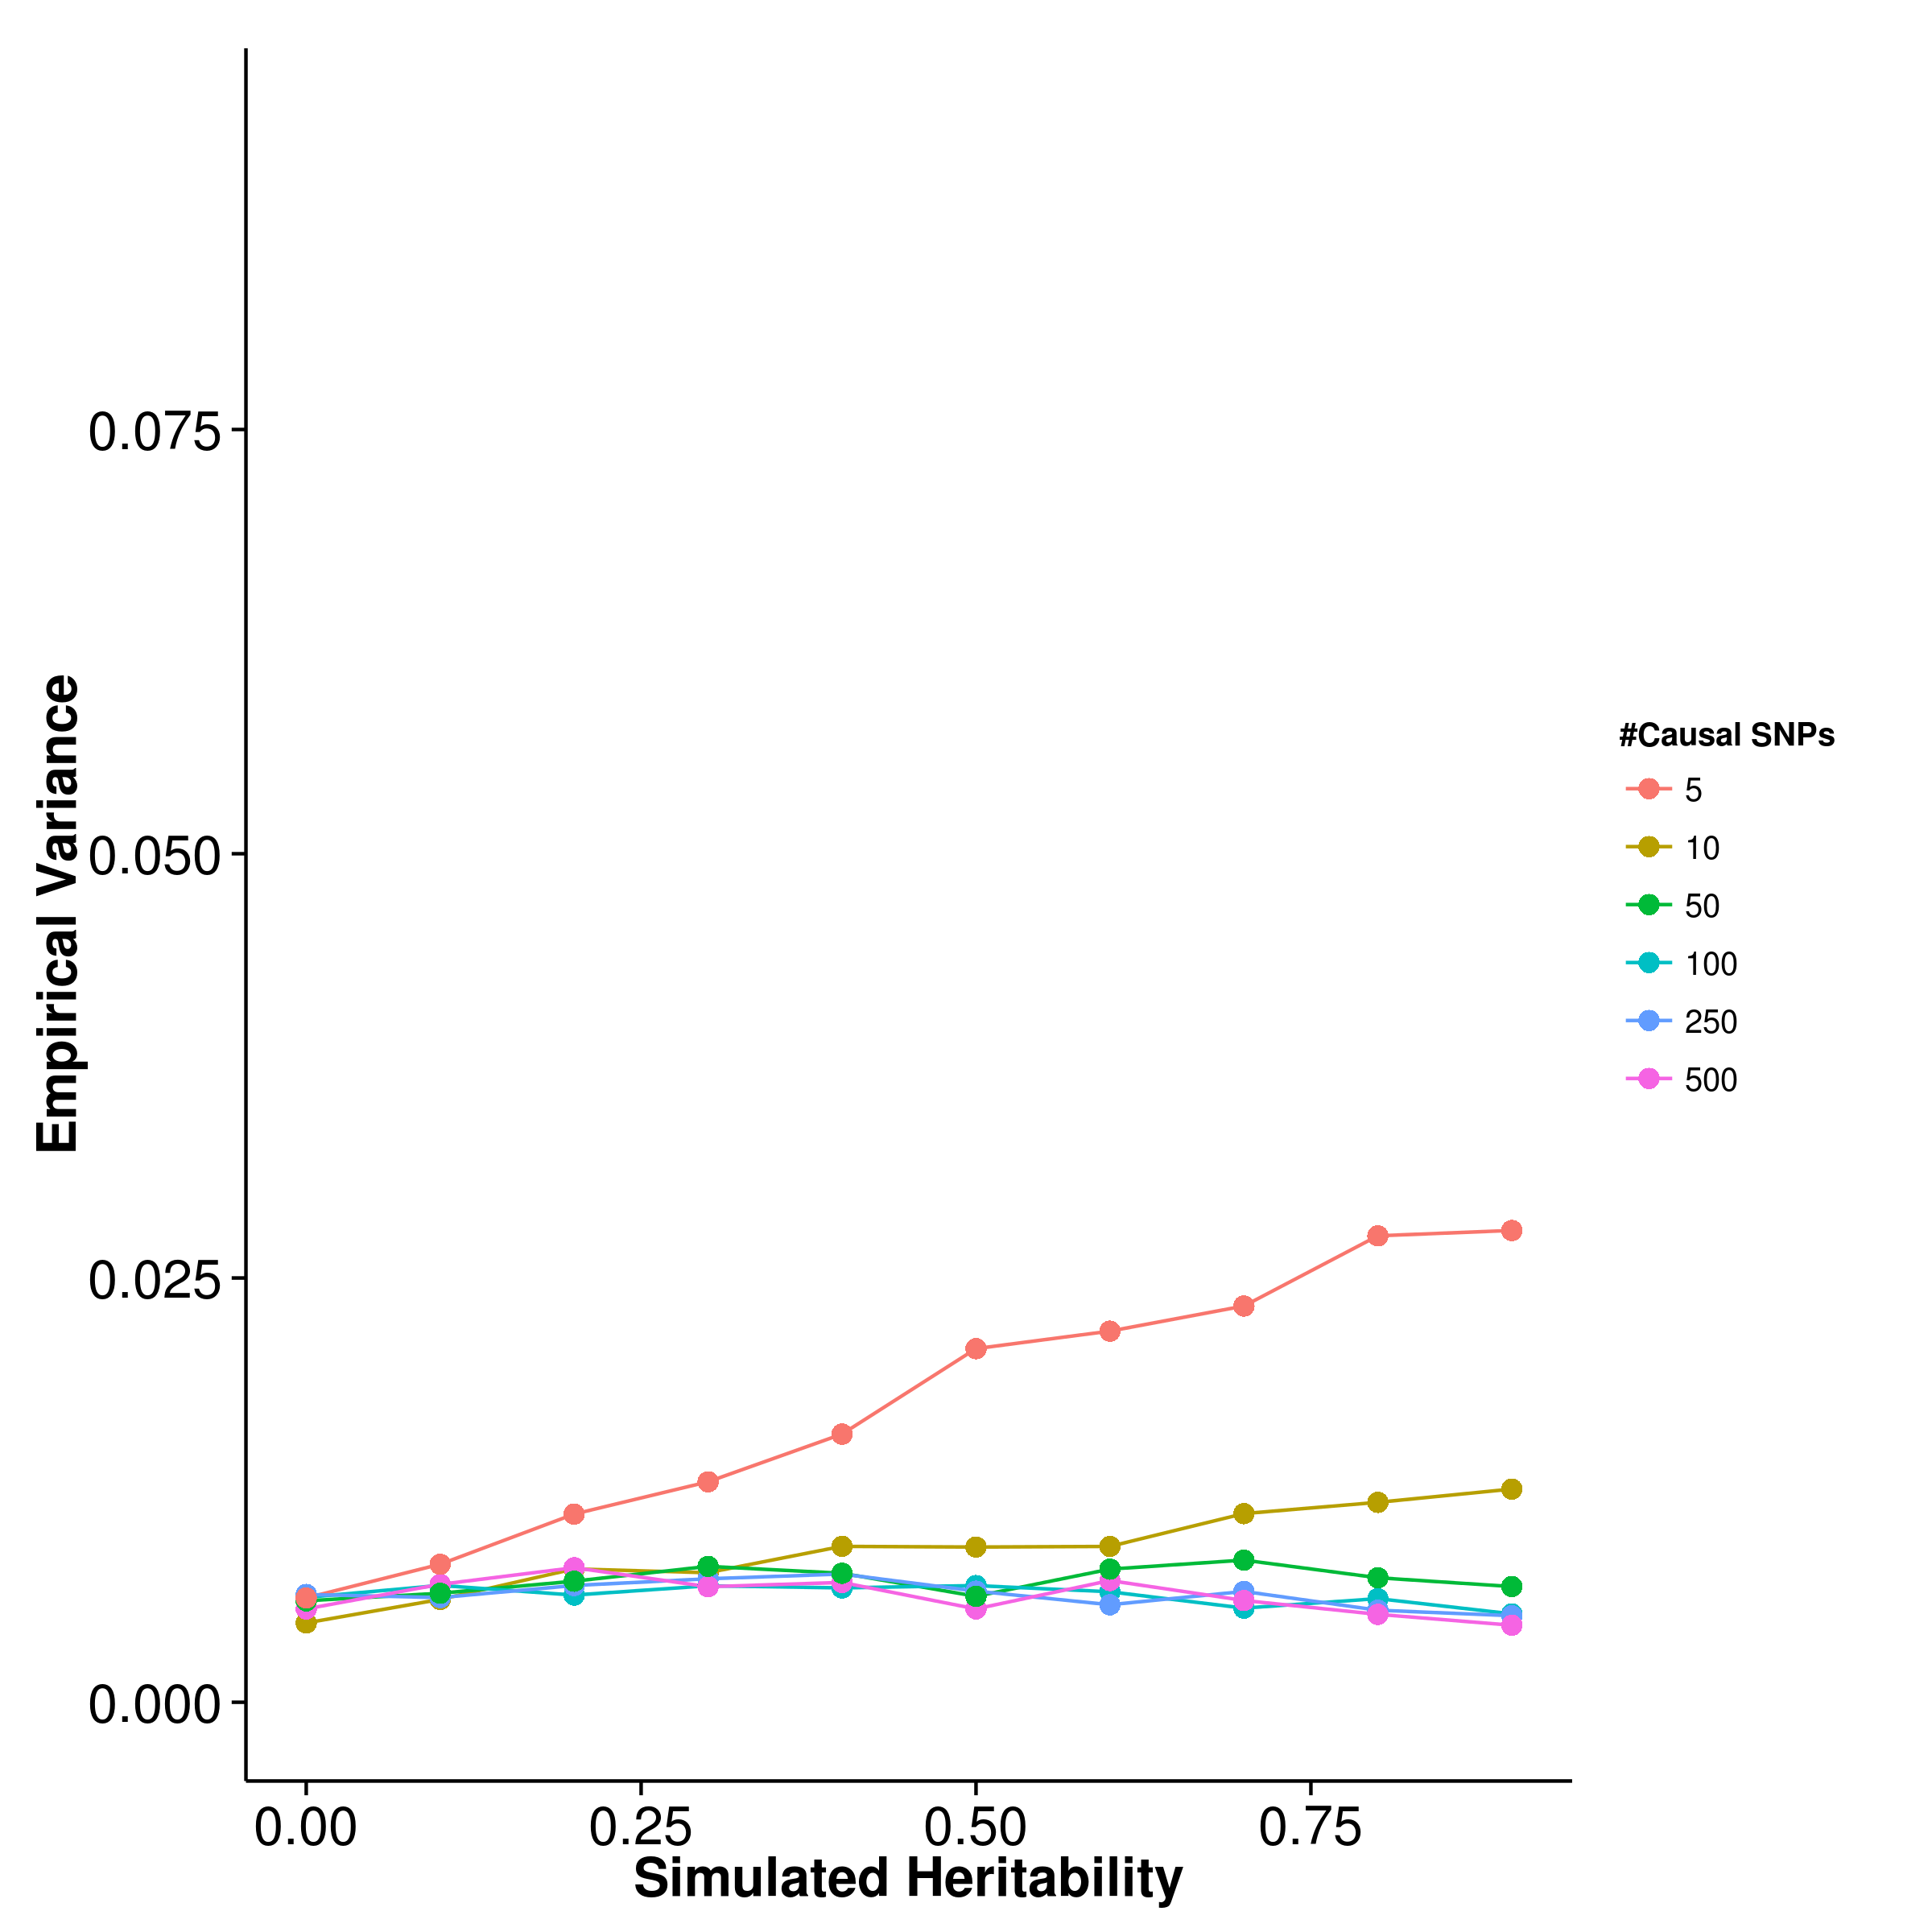
\includegraphics{figure/he_summary/equal/gcta_Qt_Equal_sd.png}}
				\label{fig:gctaQtEqualVar}
			}\\
			\subfloat[LDSC with fix intercept]{
				\scalebox{.4}{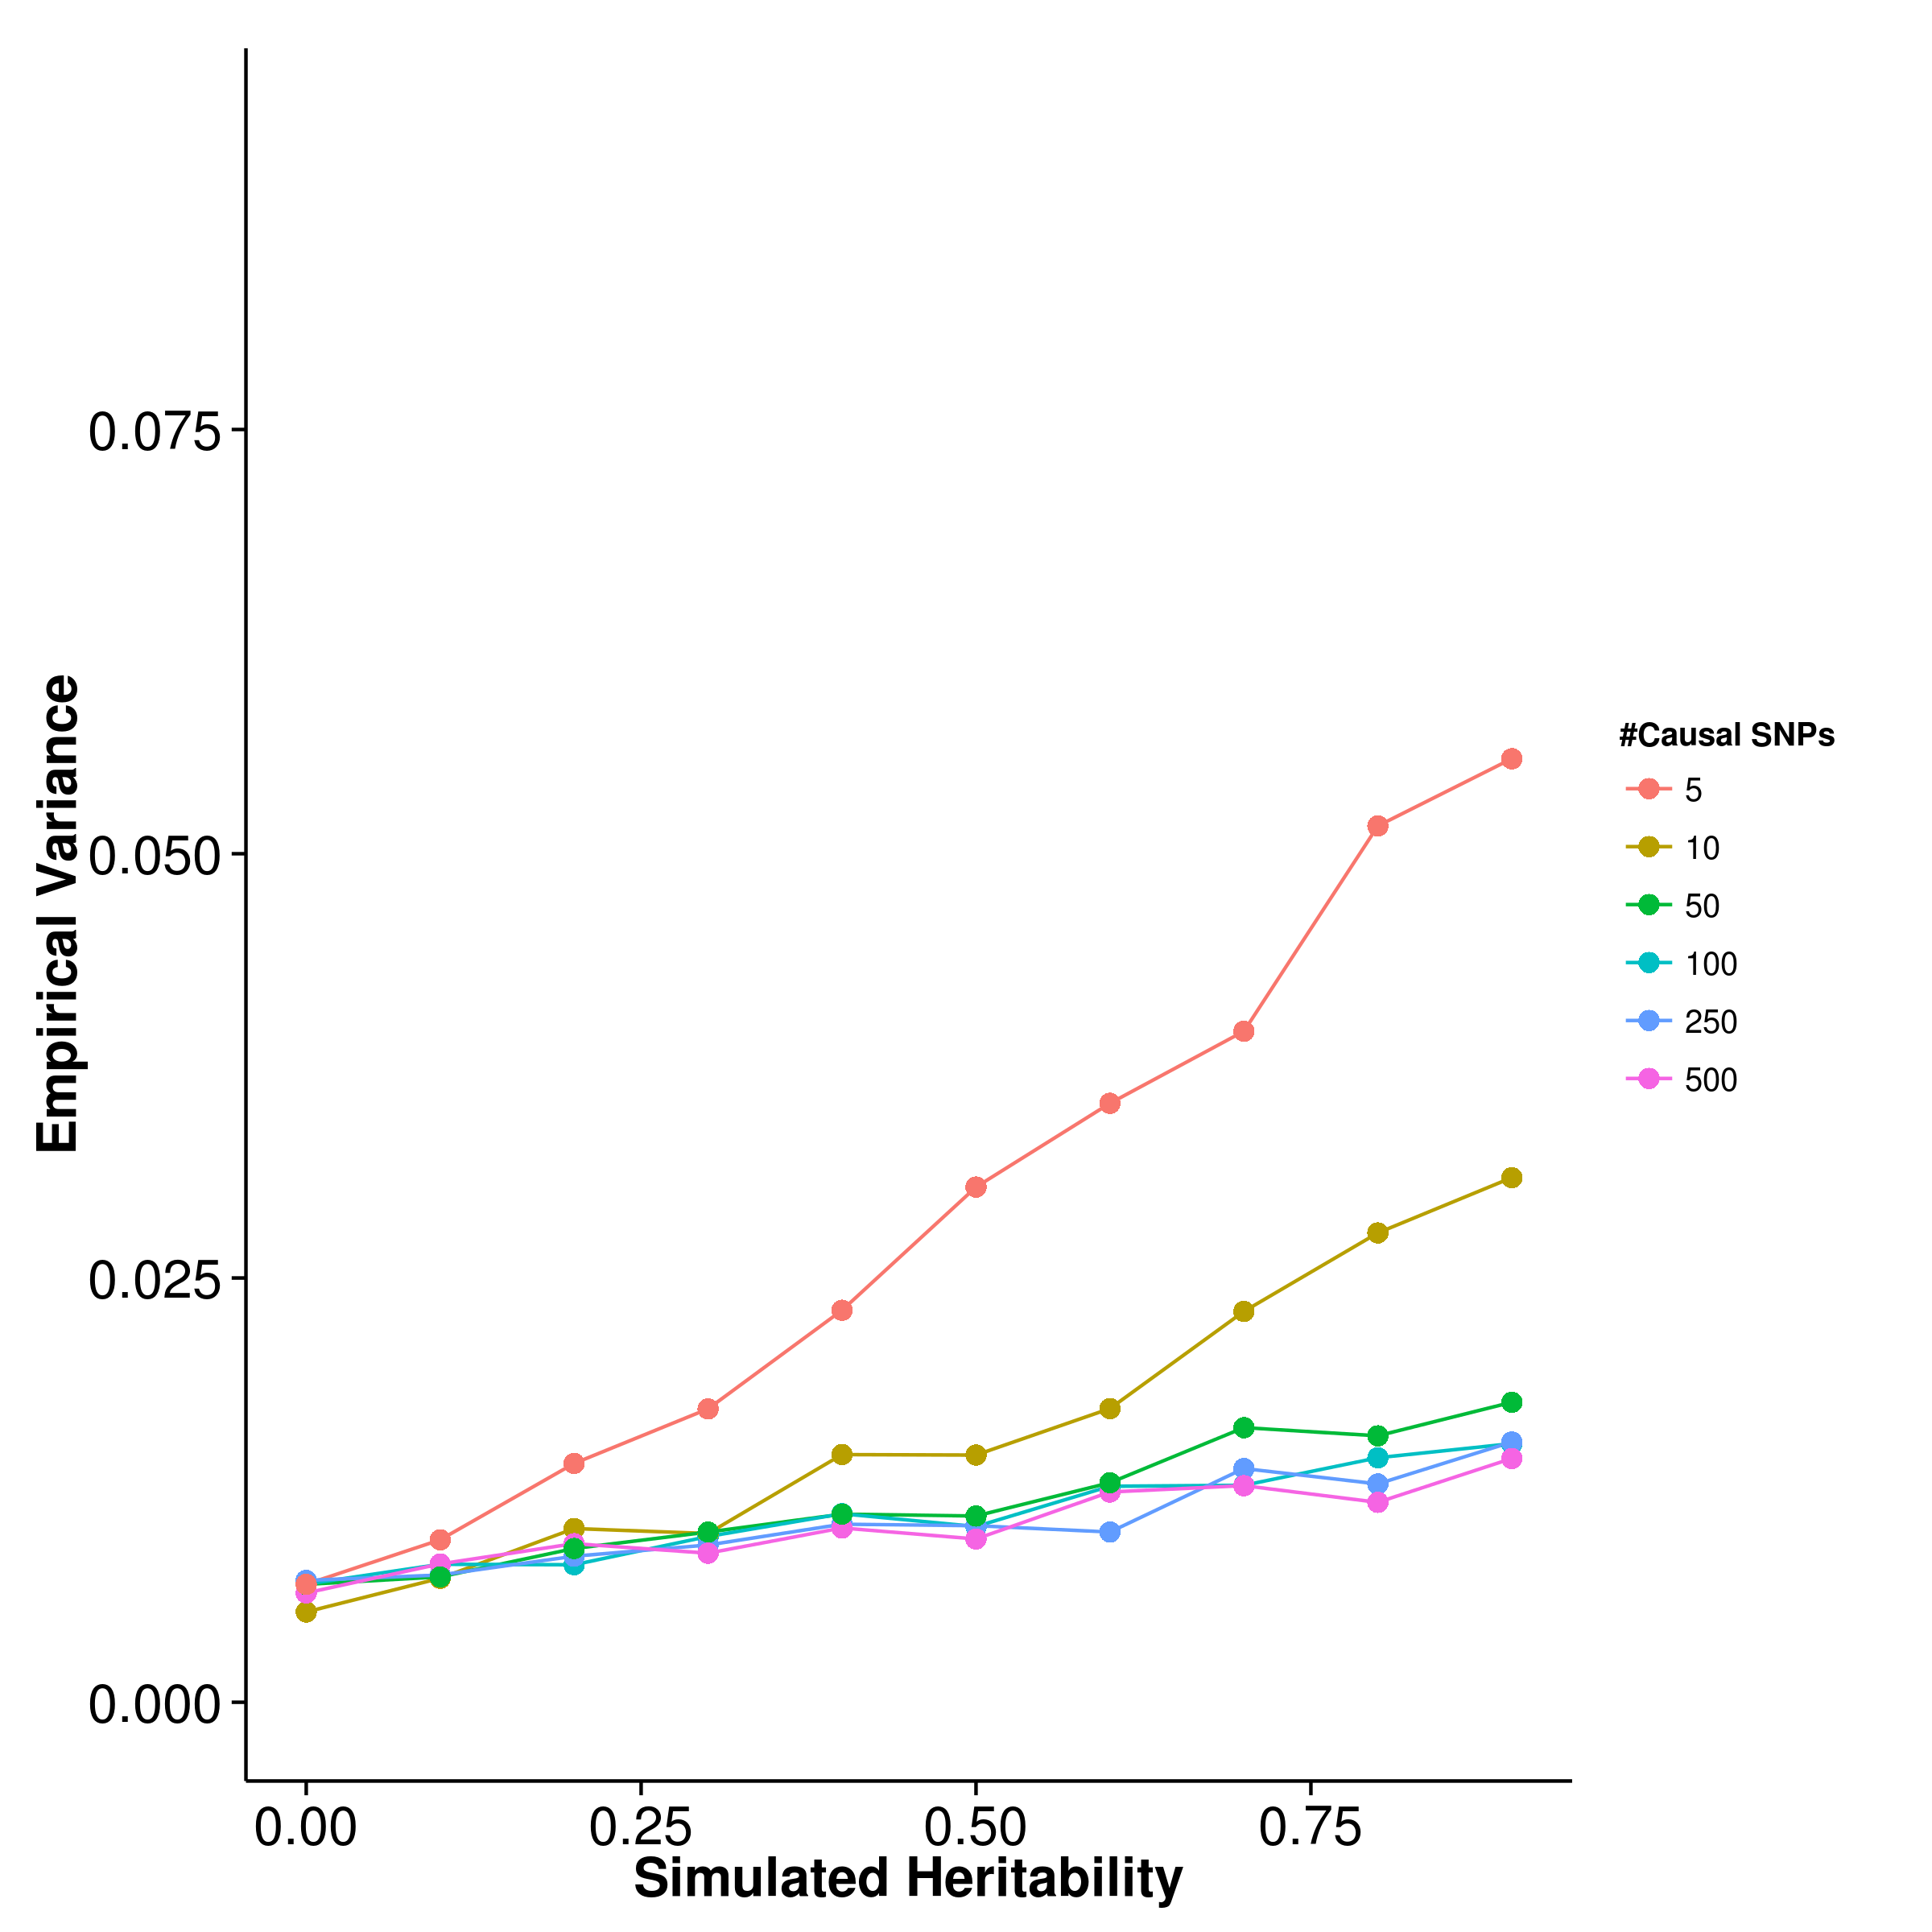
\includegraphics{figure/he_summary/equal/ldsc_Qt_Equal_sd.png}}
				\label{fig:ldscQtEqualVar}
			}
			\subfloat[LDSC with intercept estimation]{
				
				\scalebox{.4}{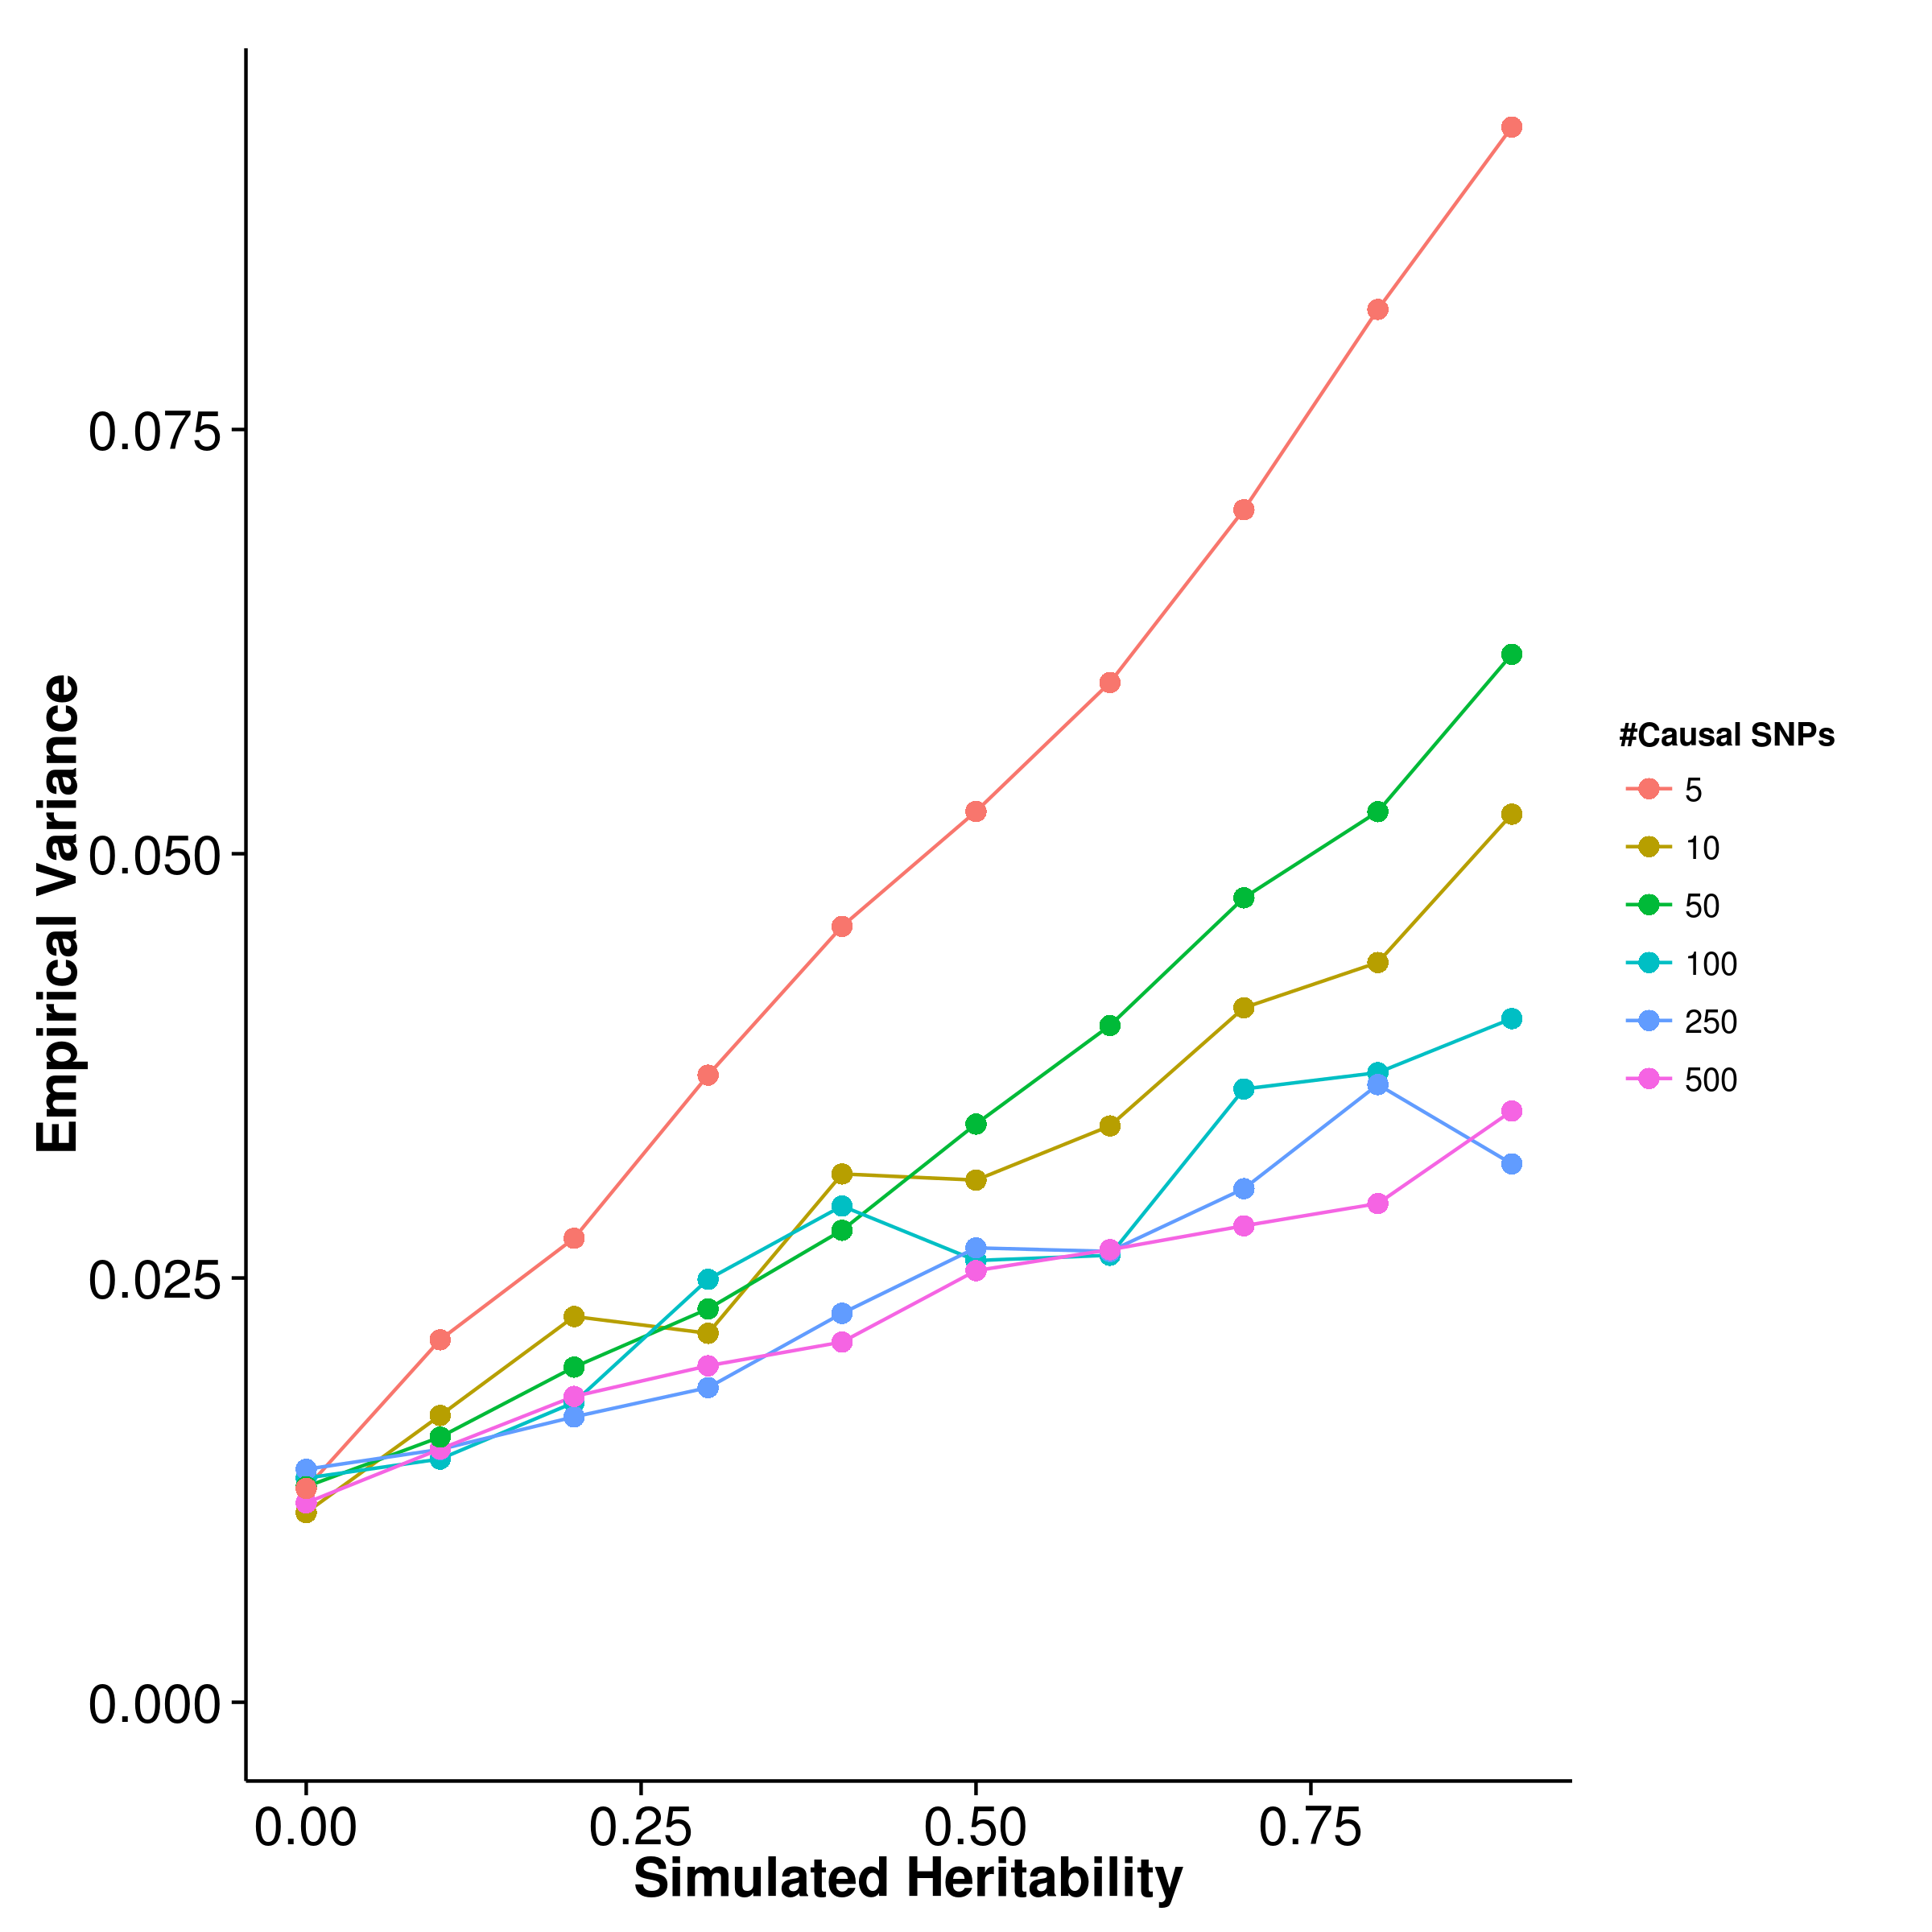
\includegraphics{figure/he_summary/equal/ldscIn_Qt_Equal_sd.png}}
				\label{fig:ldscInQtEqualVar}
			}
			\caption[Quantitative Trait with Equal Effect Size Simulation Result(Variance)]
			{Variance of results from quantitative trait simulation with equal effect size simulation.
				Of all the programmes, \gls{gcta} was found to have the lowest variance, follow by \gls{ldsc} with fixed intercept.
				The variance of \gls{shrek} was slightly higher than that of \gls{ldsc} with fixed intercept and is lower than that of \gls{ldsc} with intercept estimation.
				Unlike \gls{ldsc}, the variance of \gls{shrek} was less sensitive to change in total heritability.} 
			\label{fig:QtEqualVar}
		\end{figure}
		
		\begin{figure}
			\centering
			\subfloat[SHREK]{
				\scalebox{.4}{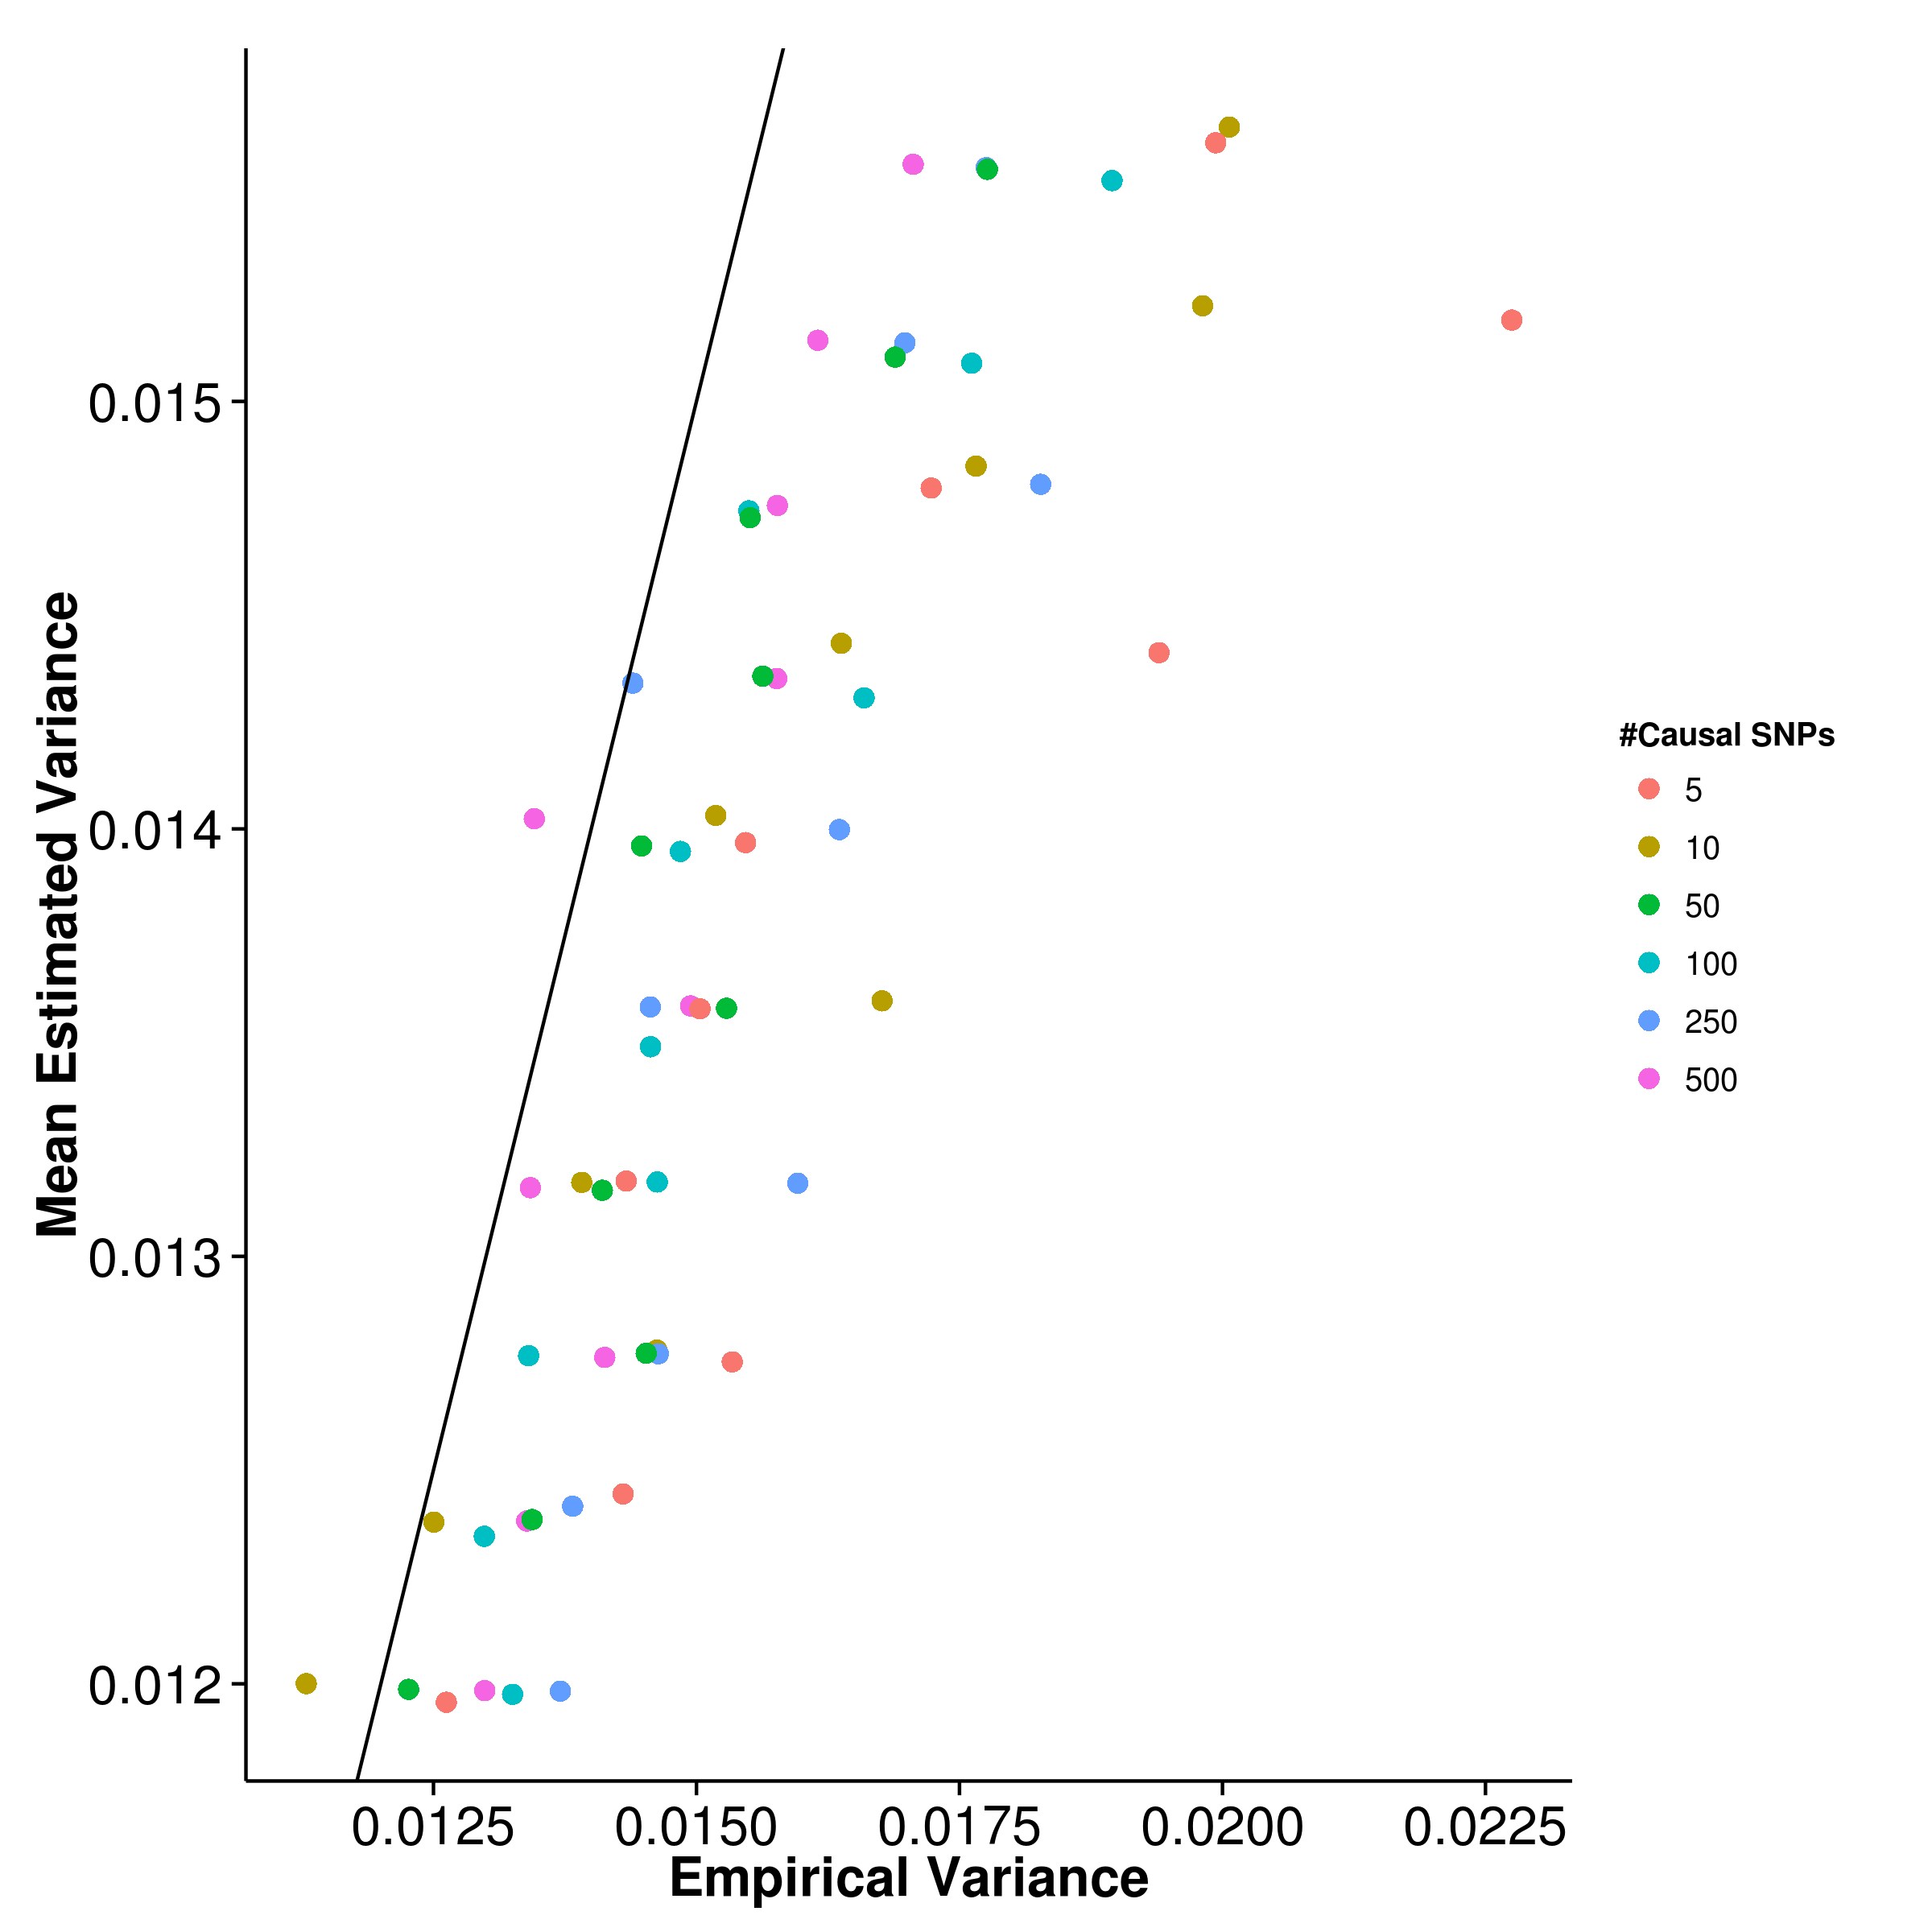
\includegraphics{figure/he_summary/equal/shrek_Qt_Equal_sdCom.png}}
				\label{fig:shrekQtEqualVarCom}
			}
			\subfloat[GCTA]{
				\scalebox{.4}{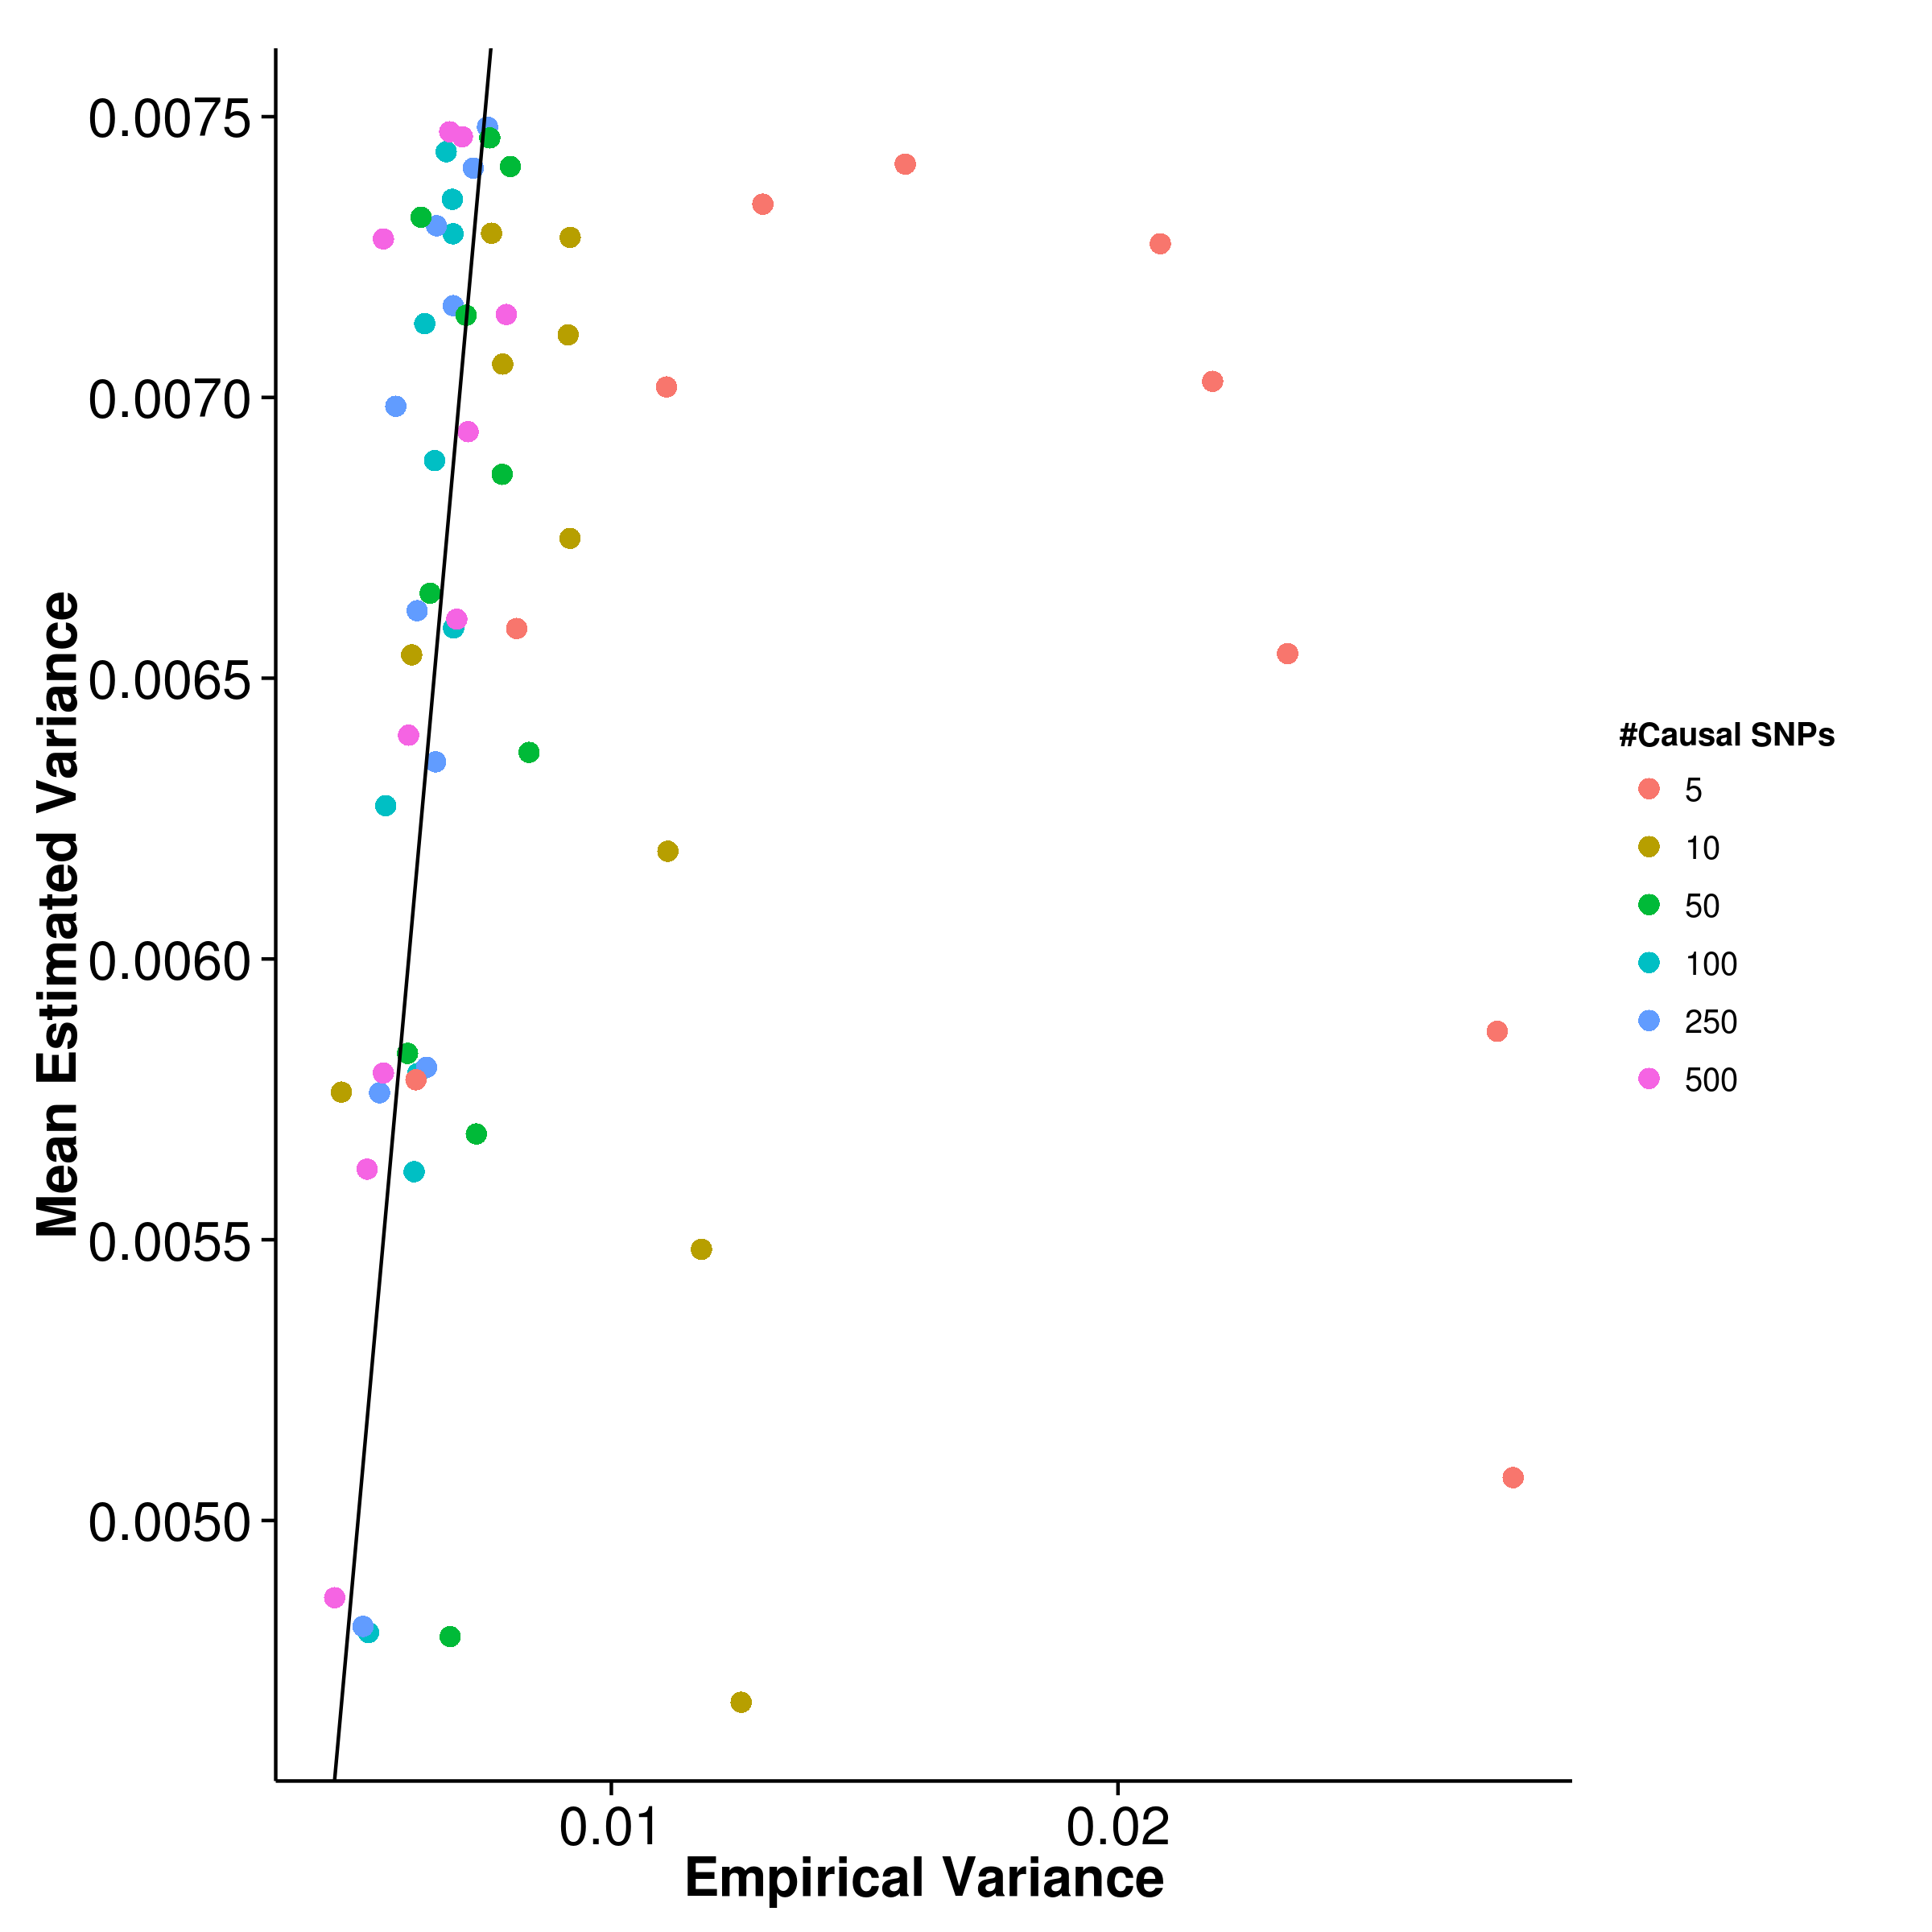
\includegraphics{figure/he_summary/equal/gcta_Qt_Equal_sdCom.png}}
				\label{fig:gctaQtEqualVarCom}
			}\\
			\subfloat[LDSC with fix intercept]{
				\scalebox{.4}{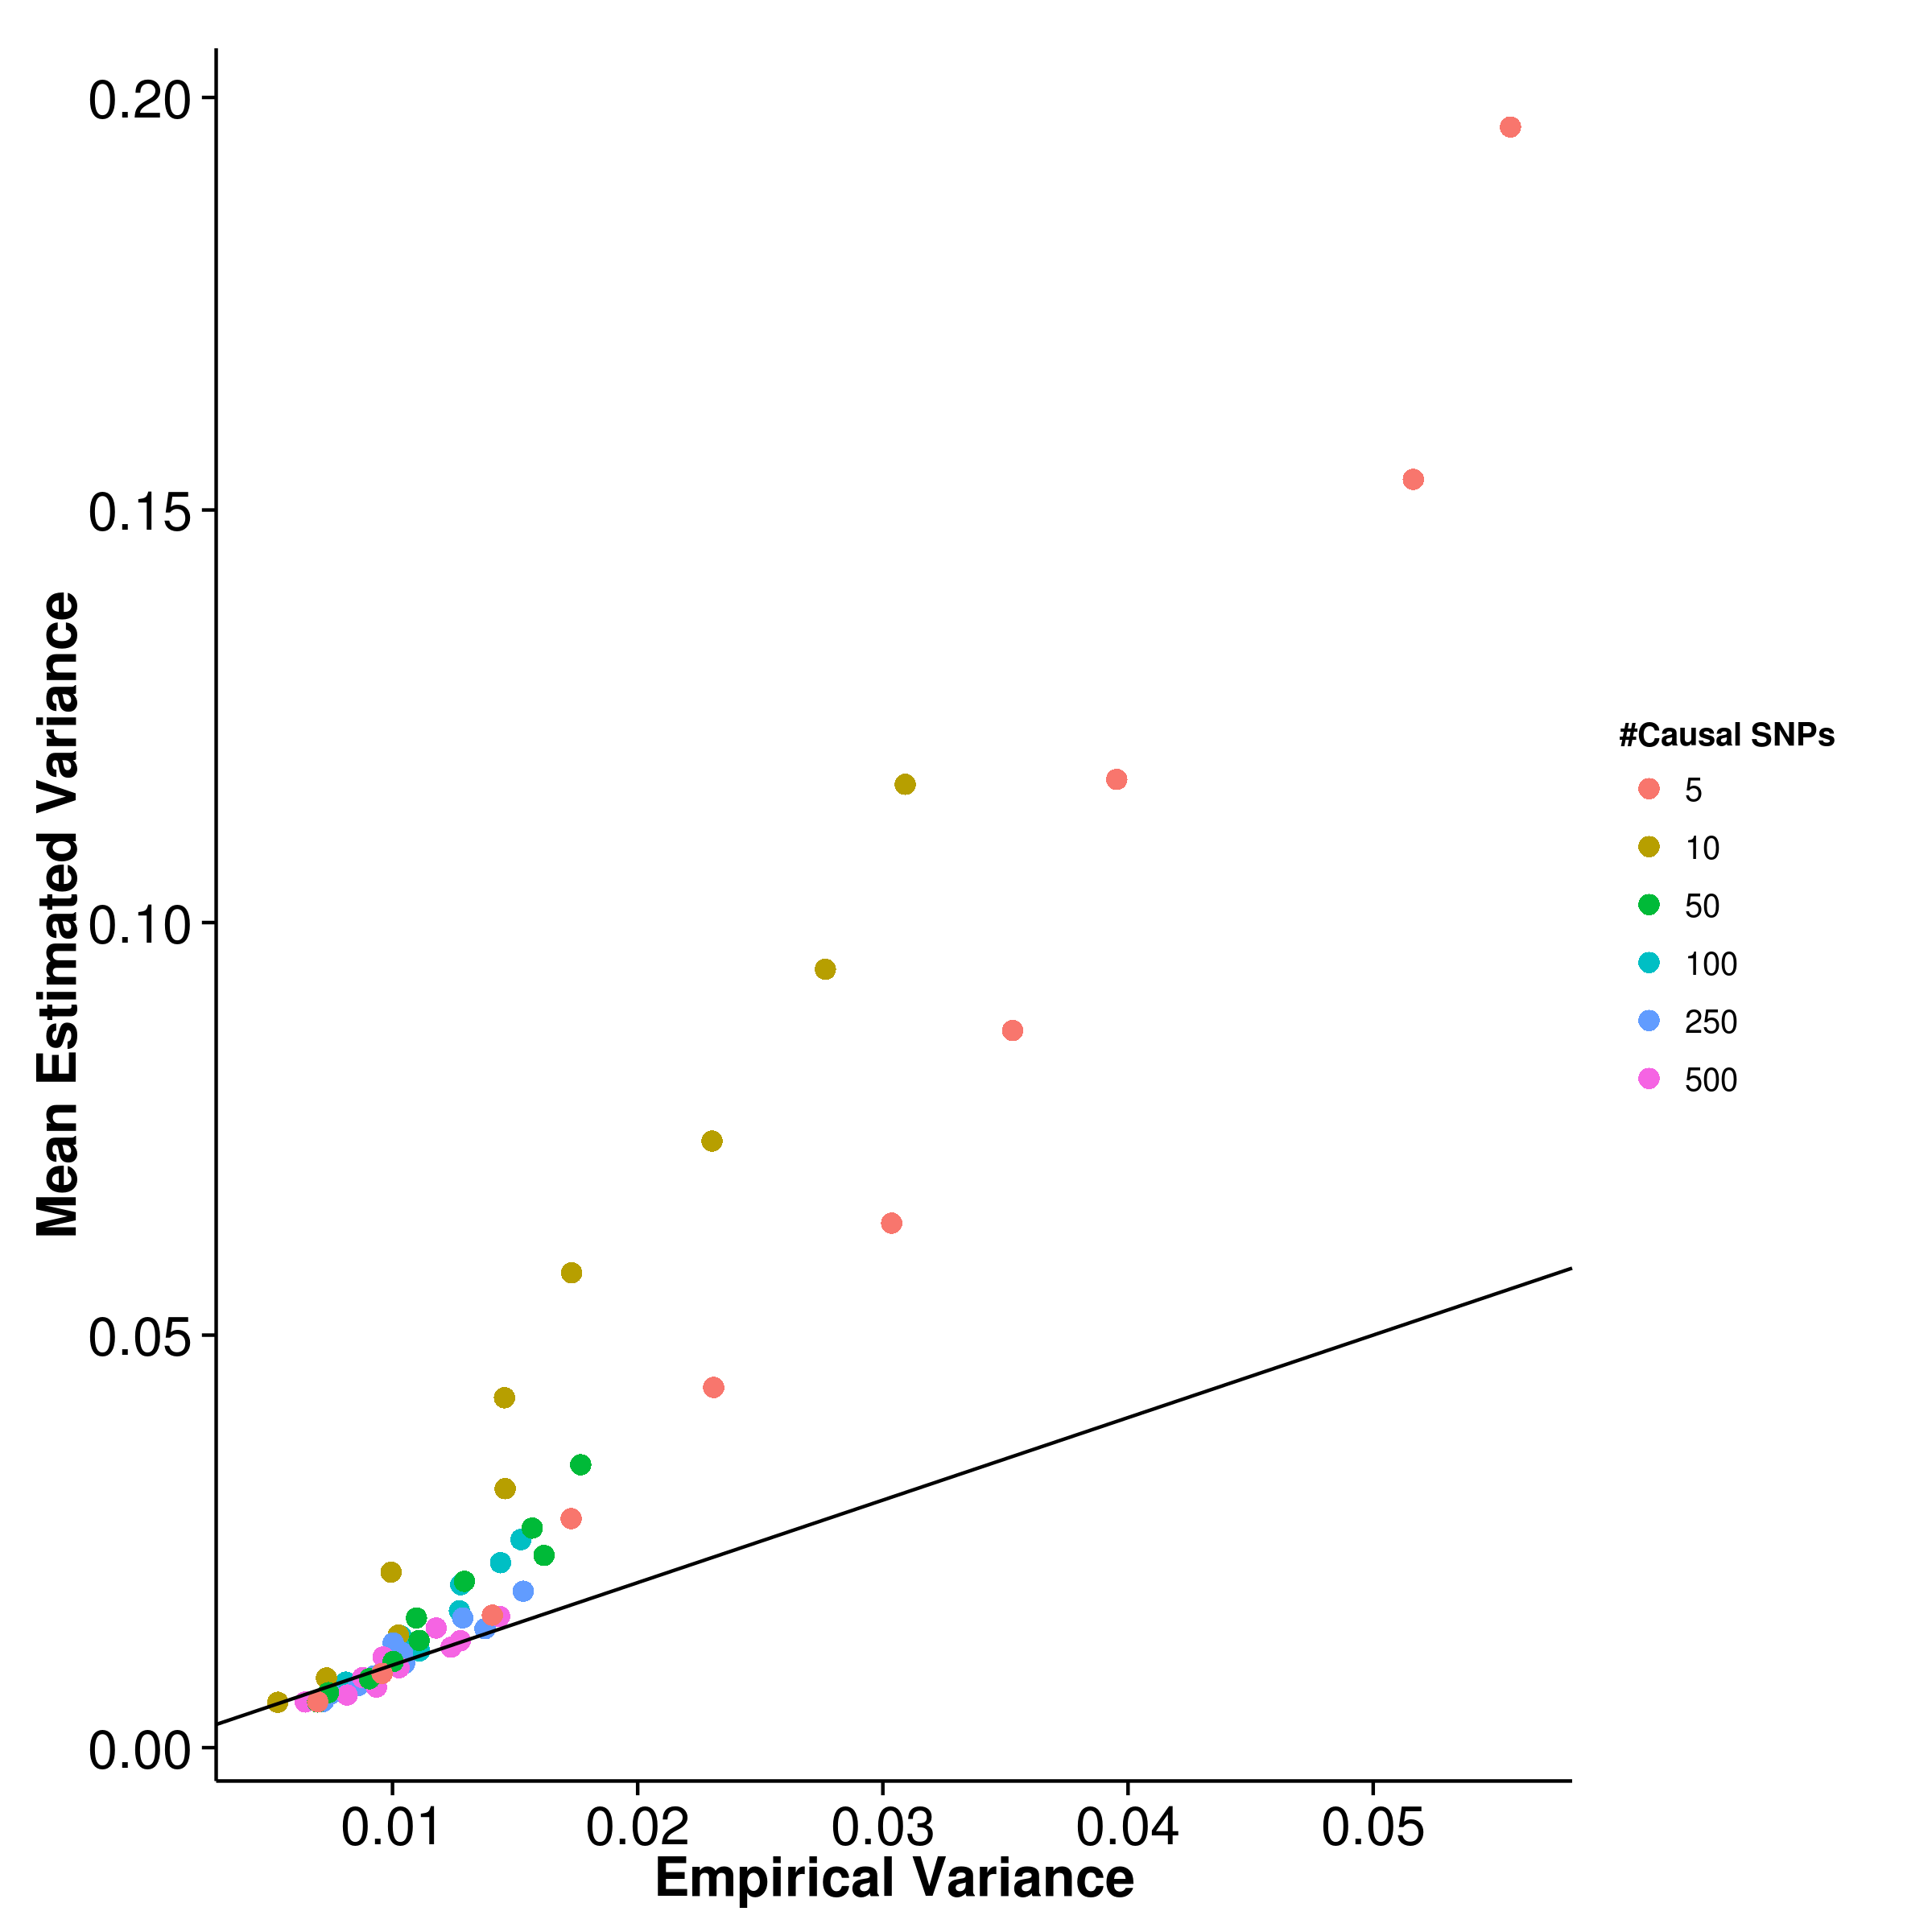
\includegraphics{figure/he_summary/equal/ldsc_Qt_Equal_sdCom.png}}
				\label{fig:ldscQtEqualVarCom}
			}
			\subfloat[LDSC with intercept estimation]{
				
				\scalebox{.4}{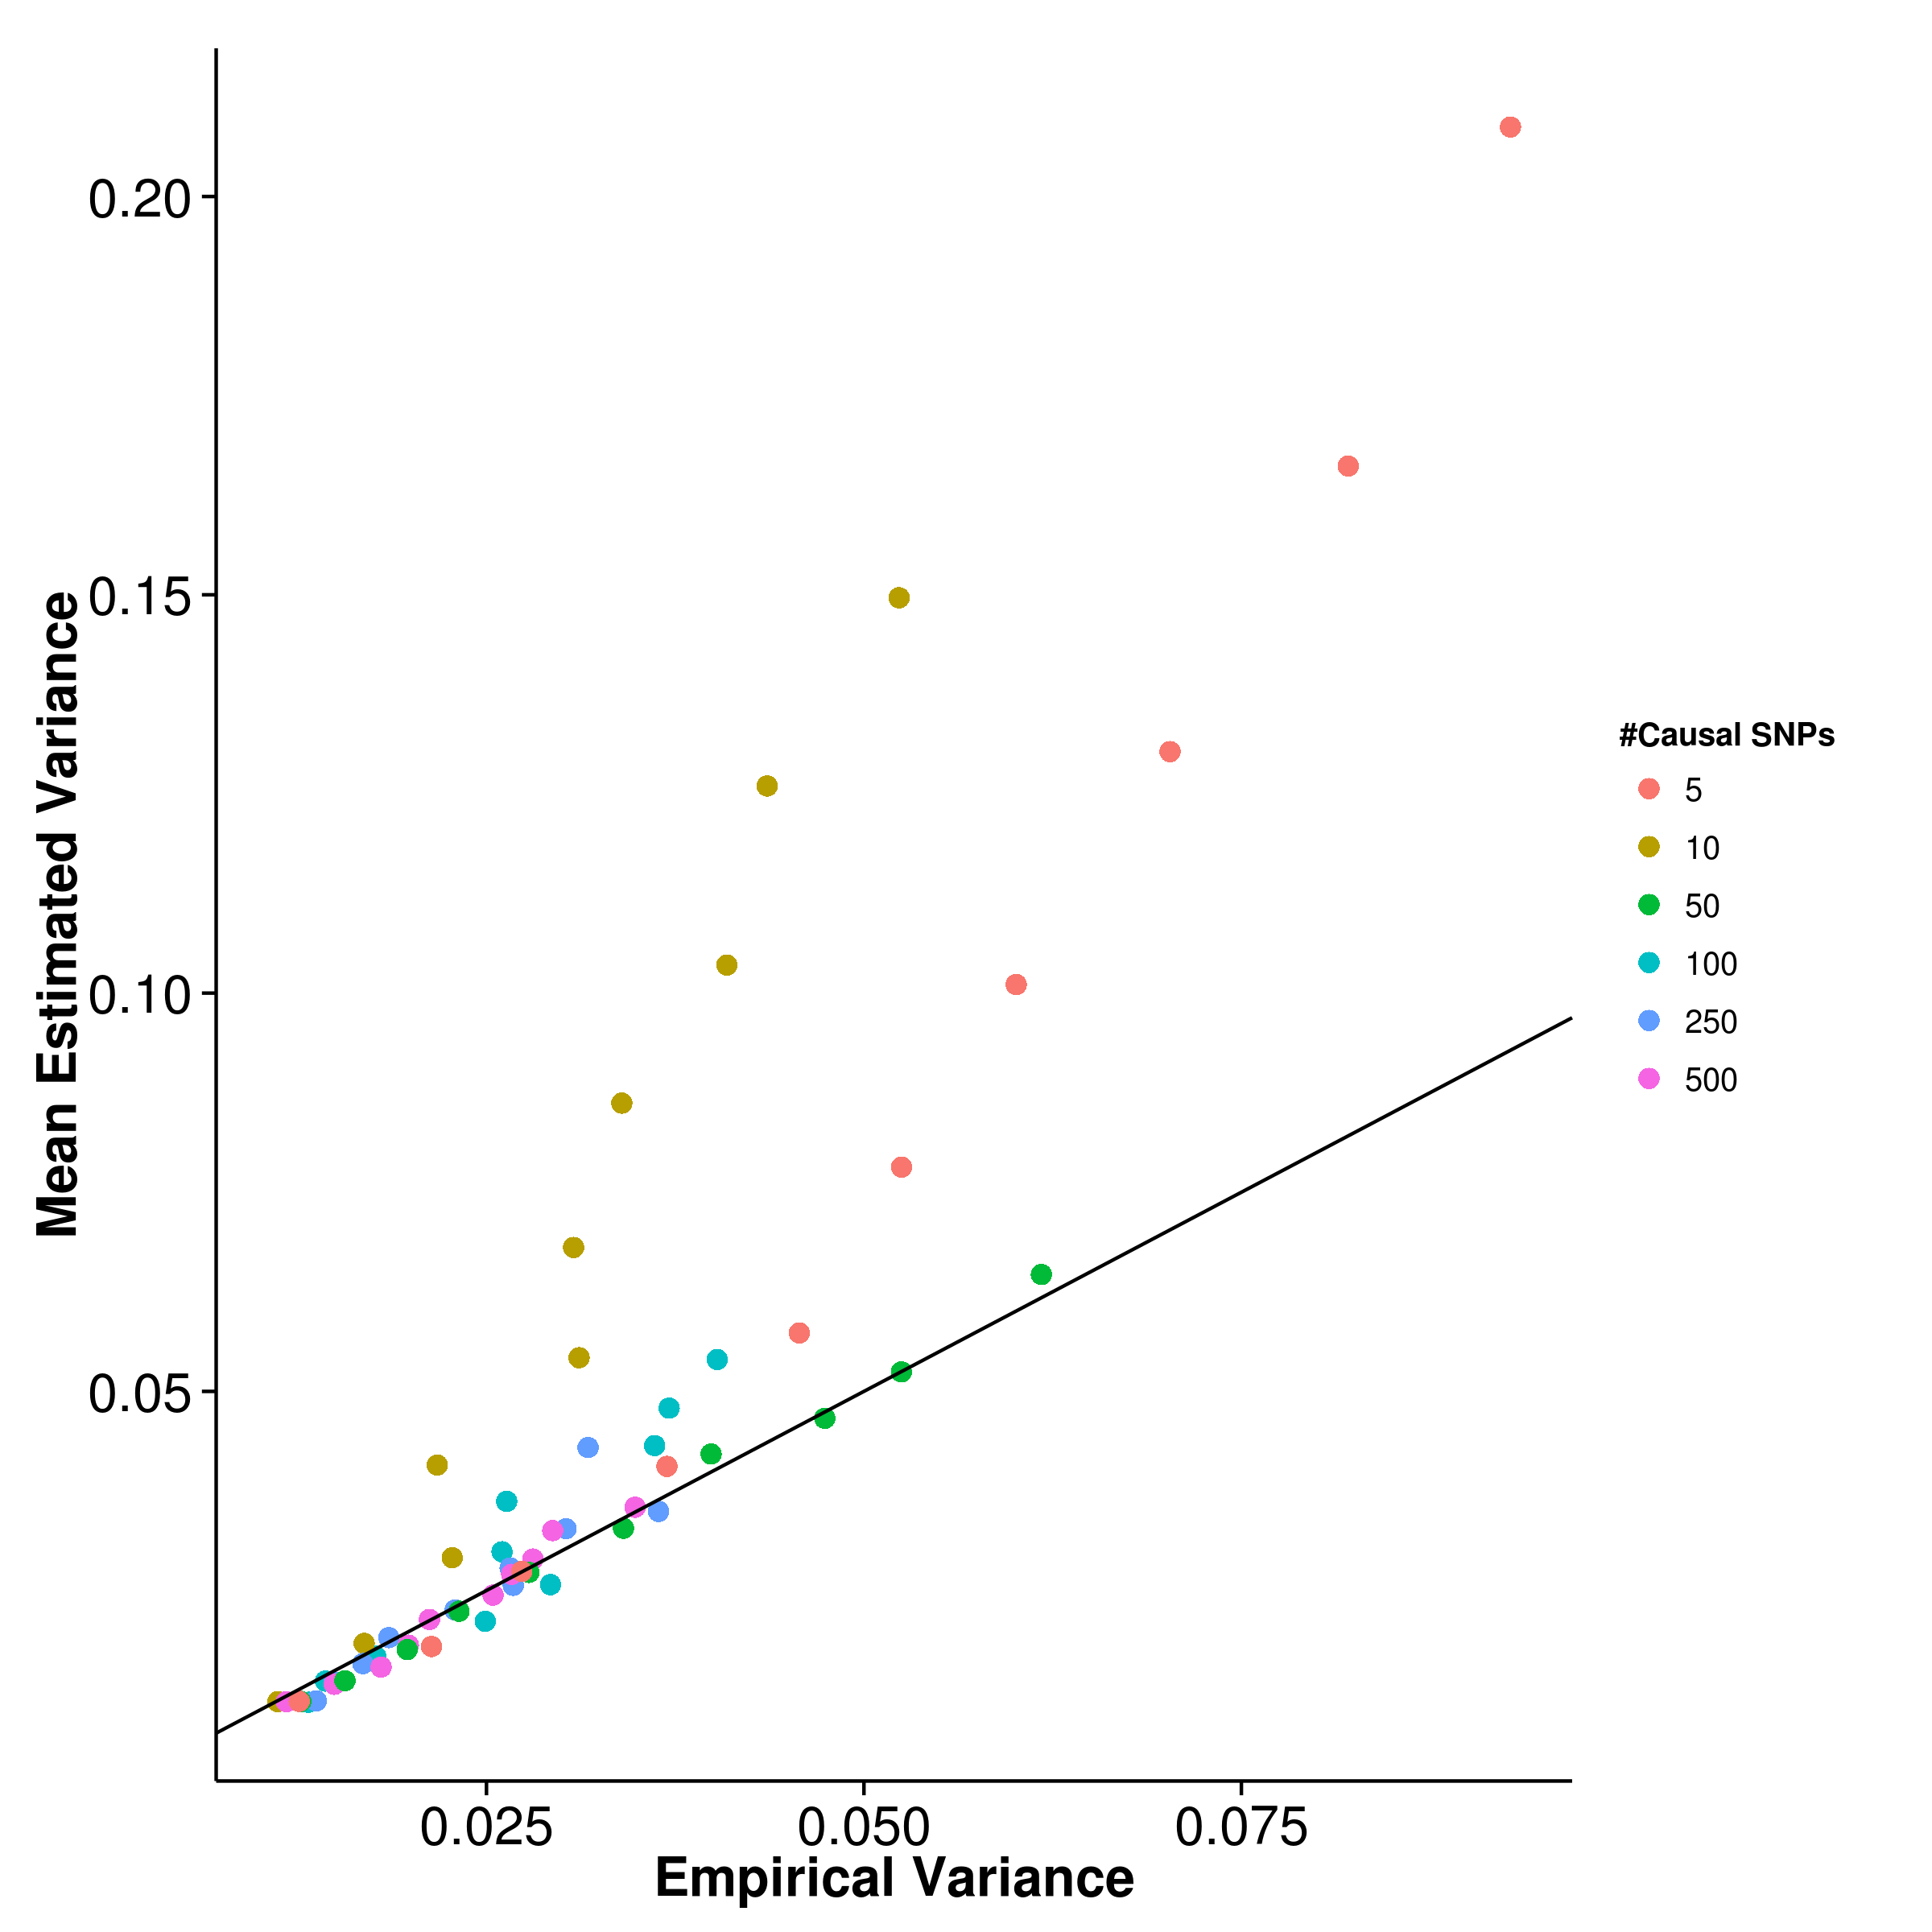
\includegraphics{figure/he_summary/equal/ldscIn_Qt_Equal_sdCom.png}}
				\label{fig:ldscInQtEqualVarCom}
			}
			\caption[Quantitative Trait with Equal Effect Size Simulation Result(Estimated Variance)]
			{Estimated variance of results from quantitative trait simulation with equal effect size simulation compared to the empirical variance.
				The estimated variances of all the tools were rather sensitive to the number of causal \glspl{SNP}, where \gls{ldsc} tends to over-estimate the variance as the number of causal \glspl{SNP} decreases and \gls{shrek} and \gls{gcta} tends to under-estimate the variance.} 
			\label{fig:QtEqualVarCom}
		\end{figure}
		The simulation of equal effect size serves as a simplistic baseline model for the performance of the programmes.
		The first thing to look at is the mean estimation of heritability of the programmes.
		If there is any bias in the estimation of the programmes, one can easily visualize it by plotting the mean estimated heritability against the simulated heritability(\cref{fig:QtEqualMean}).
		
		From the graph, it is clear that there was a slight over estimation for \gls{ldsc} with fixed intercept(\cref{fig:ldscQtEqualMean}).
		The over estimation seems to be a function of the simulated heritability, where a large inflation was observed when a larger heritability was simulated.
		On the other hand, when allow for the estimation of intercept, less bias was observed for \gls{ldsc} except for the scenario where only 5 causal \glspl{SNP} was simulated where the estimation was downwardly biased.
		
		Comparing to \gls{ldsc}, \gls{shrek} has a smaller bias and tends to slightly under-estimate(\cref{fig:shrekQtEqualMean}).
		However, the bias of \gls{shrek} is insensitive to the simulated heritability, making it robust to traits with different heritability.
		Similarly, the bias of \gls{gcta} is also smaller than that of \gls{ldsc}(\cref{fig:shrekQtEqualMean}), with a slight upward bias in the estimation except when 5 causal \glspl{SNP} was simulated.
		Again, the estimate of \gls{gcta} is also relatively insensitive to the simulated heritability.
		Overall, there was no clear pattern as to how the number of causal \glspl{SNP} affects the mean estimation. 
		
		Next, we examine the empirical variance of the programmes(\cref{fig:QtEqualVar}).
		As can be seen from the graph, there is a clear pattern where the decrease in number of causal \gls{SNP} generally increases the variance for all the programmes, with \gls{shrek} least affected.
		For \gls{ldsc}, the simulated heritability also have a large impact to its empirical variance, with the empirical variance increases as the simulated heritability increases.
		In general, \gls{ldsc} with fixed intercept(\cref{fig:ldscQtEqualVar}) has a lower variance when compared to \gls{ldsc} with intercept estimation(\cref{fig:ldscInQtEqualVar}). 
		Moreover, when the number of causal \gls{SNP} is large, the variance of \gls{ldsc} with fixed intercept(\cref{fig:ldscQtEqualVar}) is lower than \gls{shrek}(\cref{fig:shrekQtEqualVar}).
		However, \gls{shrek} is more robust to change in the number of causal \glspl{SNP} and simulated heritabiliy when compared ot \gls{ldsc}.

		Of all the programmes, \gls{gcta} has the best performance(\cref{fig:gctaQtEqualVar}) except when the trait only contains 5 causal \glspl{SNP}. 
		Not only does it has the smallest variance, its empirical variances was almost invariant to change in simulated heritability.
		However, the case with 5 causal \glspl{SNP} serves as an out-lier. 
		It was most obvious when inspecting the relationship between the estimated variance and the empirical variance of \gls{gcta}(\cref{fig:gctaQtEqualVarCom}).
		Comparing the estimated variance and the empirical variance, it was clear that \gls{gcta} can, in most case accurately estimate its variance. 
		In the case of 5 causal \glspl{SNP} however, \gls{gcta} underestimates its variance.
		It was also observed in the case of 10 causal \glspl{SNP}, there was already a slight under-estimation of the variance, suggesting that there might be an increase in empirical variance that was not capture by \gls{gcta}.
		
		In the case of the programmes using the test statistic, it was observed that \gls{shrek} in general under-estimate the empirical variance(\cref{fig:shrekQtEqualVarCom}) for an average of 0.9 fold. 
		On the other hand, \gls{ldsc} over-estimates the variance for roughly 1.5 times when a fixed intercept(\cref{fig:ldscQtEqualVarCom}) was used and roughly 1.2 times when the intercept was estimated(\cref{fig:ldscInQtEqualVarCom}). 
		
		To summarize the results, we calculate the \gls{mse} of the estimation of heritability of the programmes under different simulation condition(\cref{tab:mseQtEqual}). 
		With the exception of the 5 causal \glspl{SNP} scenario, \gls{gcta} has the best performance, has a almost 2 fold smaller \gls{mse} when compared to \gls{shrek}.
		As the number of casual \glspl{SNP} increases, the performance of \gls{ldsc} with fixed intercept and \gls{shrek} converges where in general, \gls{shrek} has a smaller \gls{mse}.
		Interestingly, unlike \gls{ldsc}, \gls{shrek} was insensitive to change in number of causal \glspl{SNP} and its performance were relatively stable.
		
		% Describe the mean
		% Effect of heritability on the mean estimation
		% Effect of causal SNPs on the mean estimation
		% Descript the Variance
		% Effect of heritability on variance of estimate
		% Effect of number of causal SNPs on variance of estimation
		% Describe the estimated variance
		% How the number of causal SNPs affect the estimation of variance?

		\begin{table}
			\centering
			\begin{tabular}{rrrrr}
				\toprule
				Number of Causal SNPs&	SHREK&	LDSC&	LDSC-In&	GCTA \\
				\midrule
				5	&	0.167	&	0.308&	0.526&	0.177	\\
				10	&	0.158	&	0.243&	0.337&	0.0944	\\
				50	&	0.150	&	0.163&	0.354&	0.0749	\\
				100	&	0.154	&	0.161&	0.304&	0.0664	\\
				250	&	0.157	&	0.147&	0.255&	0.0659	\\
				500	&	0.147	&	0.148&	0.247&	0.0661	\\
				\bottomrule
			\end{tabular}
			\caption[Mean Squared Error of Quantitative Trait Simulation with Equal Effect Size]{
				\gls{mse} of quantitative trait simulation with equal effect size.
				It was observed that the overall \gls{mse} of \gls{gcta} is very low, follow by \gls{shrek}.
				As the number of causal \glspl{SNP} decreases, the \gls{mse} increases for all programmes. 
				The performance of \gls{shrek} and \gls{ldsc} with fixed intercept converges as the number of causal \glspl{SNP} increases.}
			\label{tab:mseQtEqual}
		\end{table}
		
		\subsection{Quantitative Trait Simulation with Random Effect Size}
		% QT Random Effect
			\begin{figure}
			\centering
			\subfloat[SHREK]{
				\scalebox{.4}{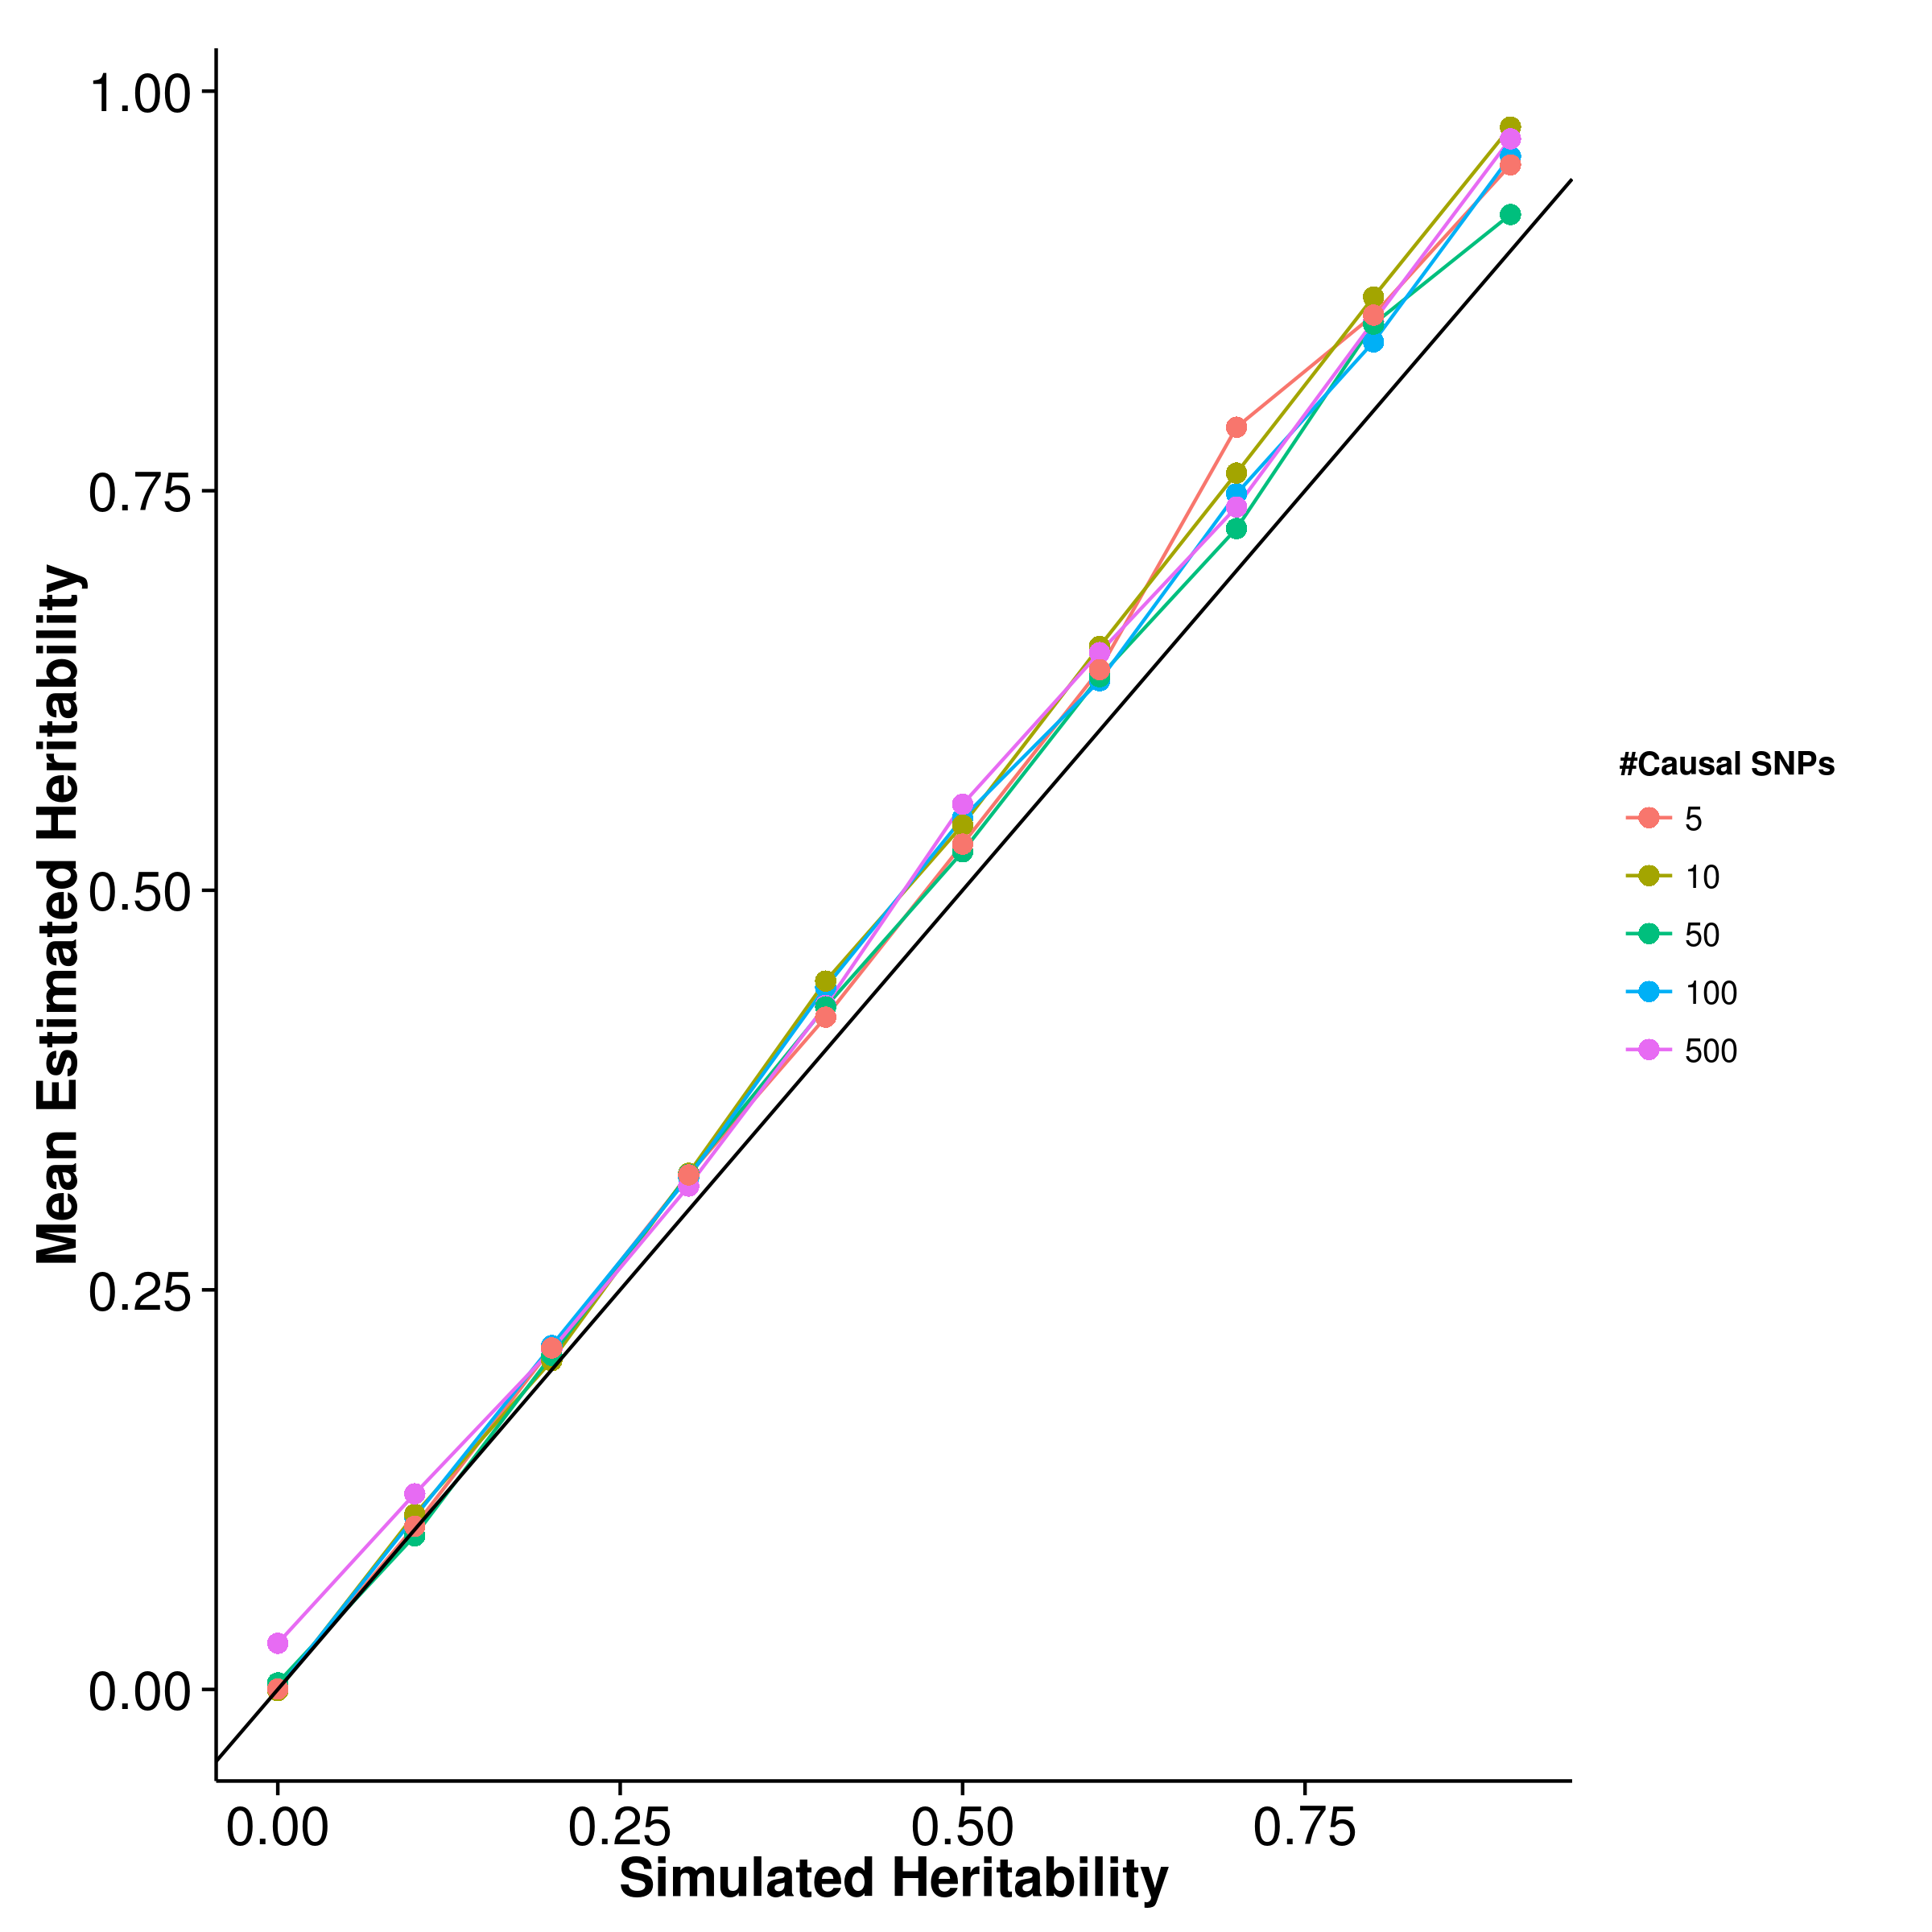
\includegraphics{figure/he_summary/random/shrek_Qt_Rand_mean.png}}
				\label{fig:shrekQtRandMean}
			}
			\subfloat[GCTA]{
				\scalebox{.4}{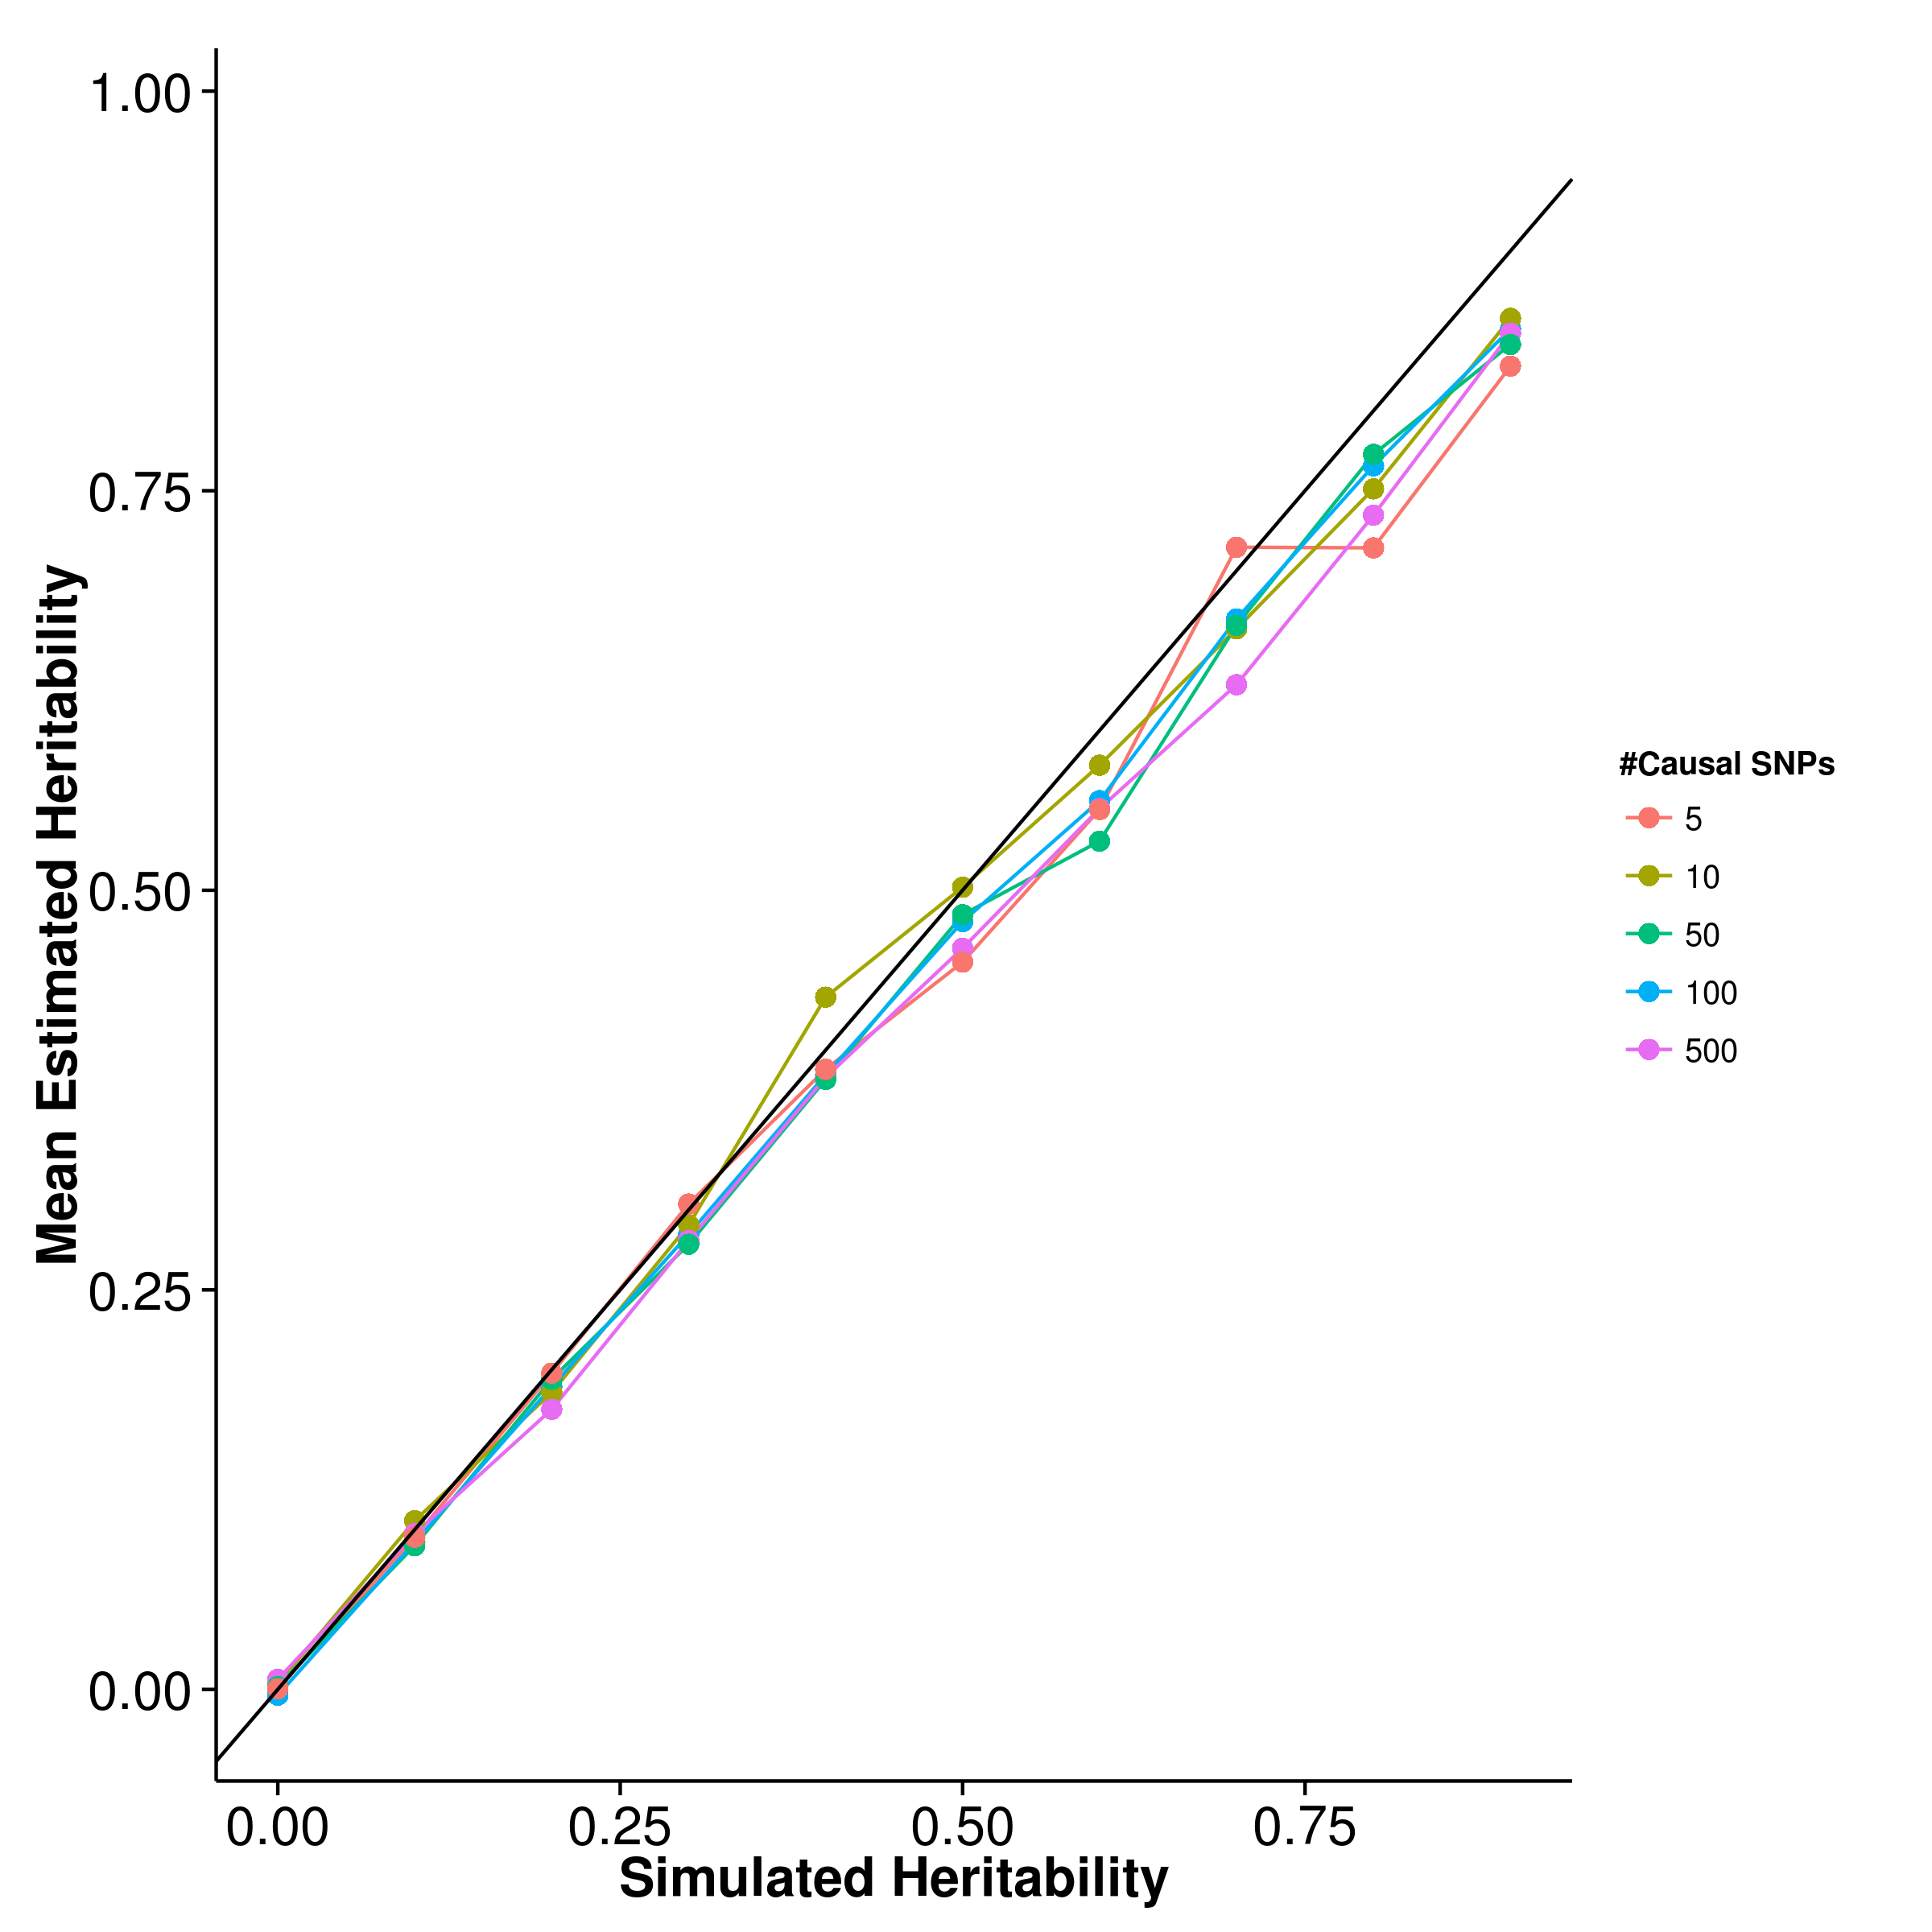
\includegraphics{figure/he_summary/random/gcta_Qt_Rand_mean.png}}
				\label{fig:gctaQtRandMean}
			}\\
			\subfloat[LDSC with fix intercept]{
				\scalebox{.4}{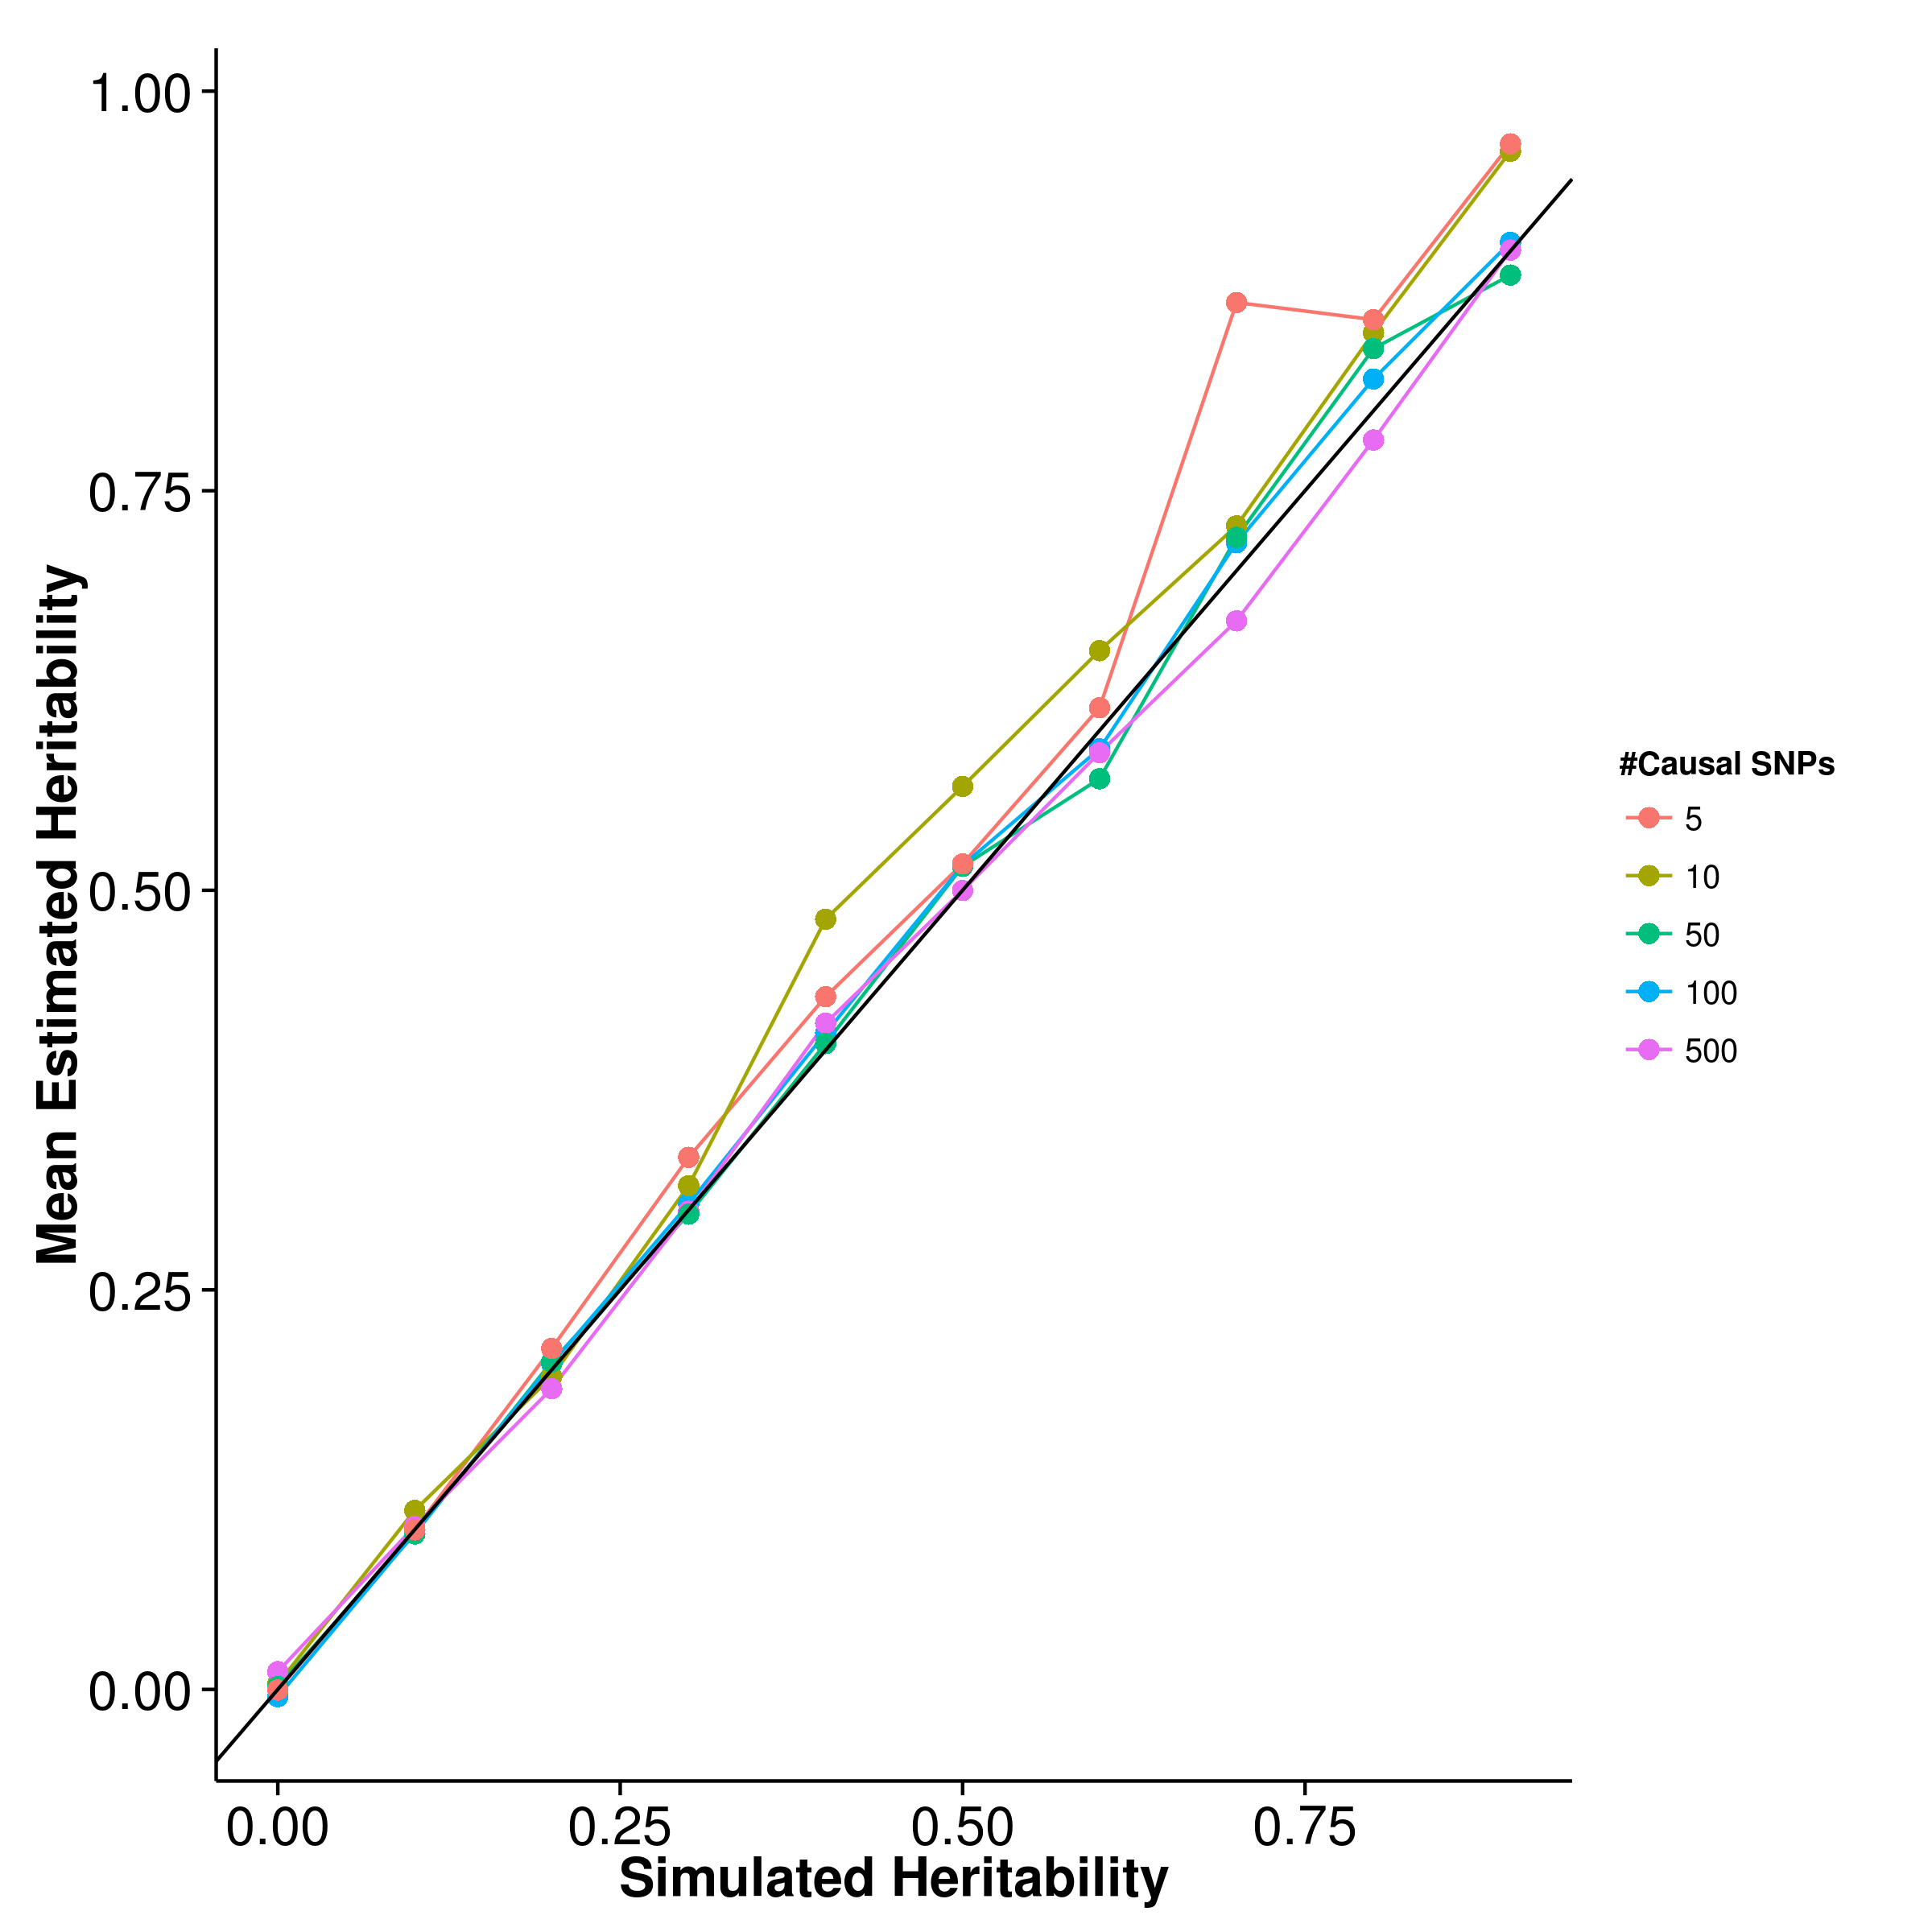
\includegraphics{figure/he_summary/random/ldsc_Qt_Rand_mean.png}}
				\label{fig:ldscQtRandMean}
			}
			\subfloat[LDSC with intercept estimation]{
				
				\scalebox{.4}{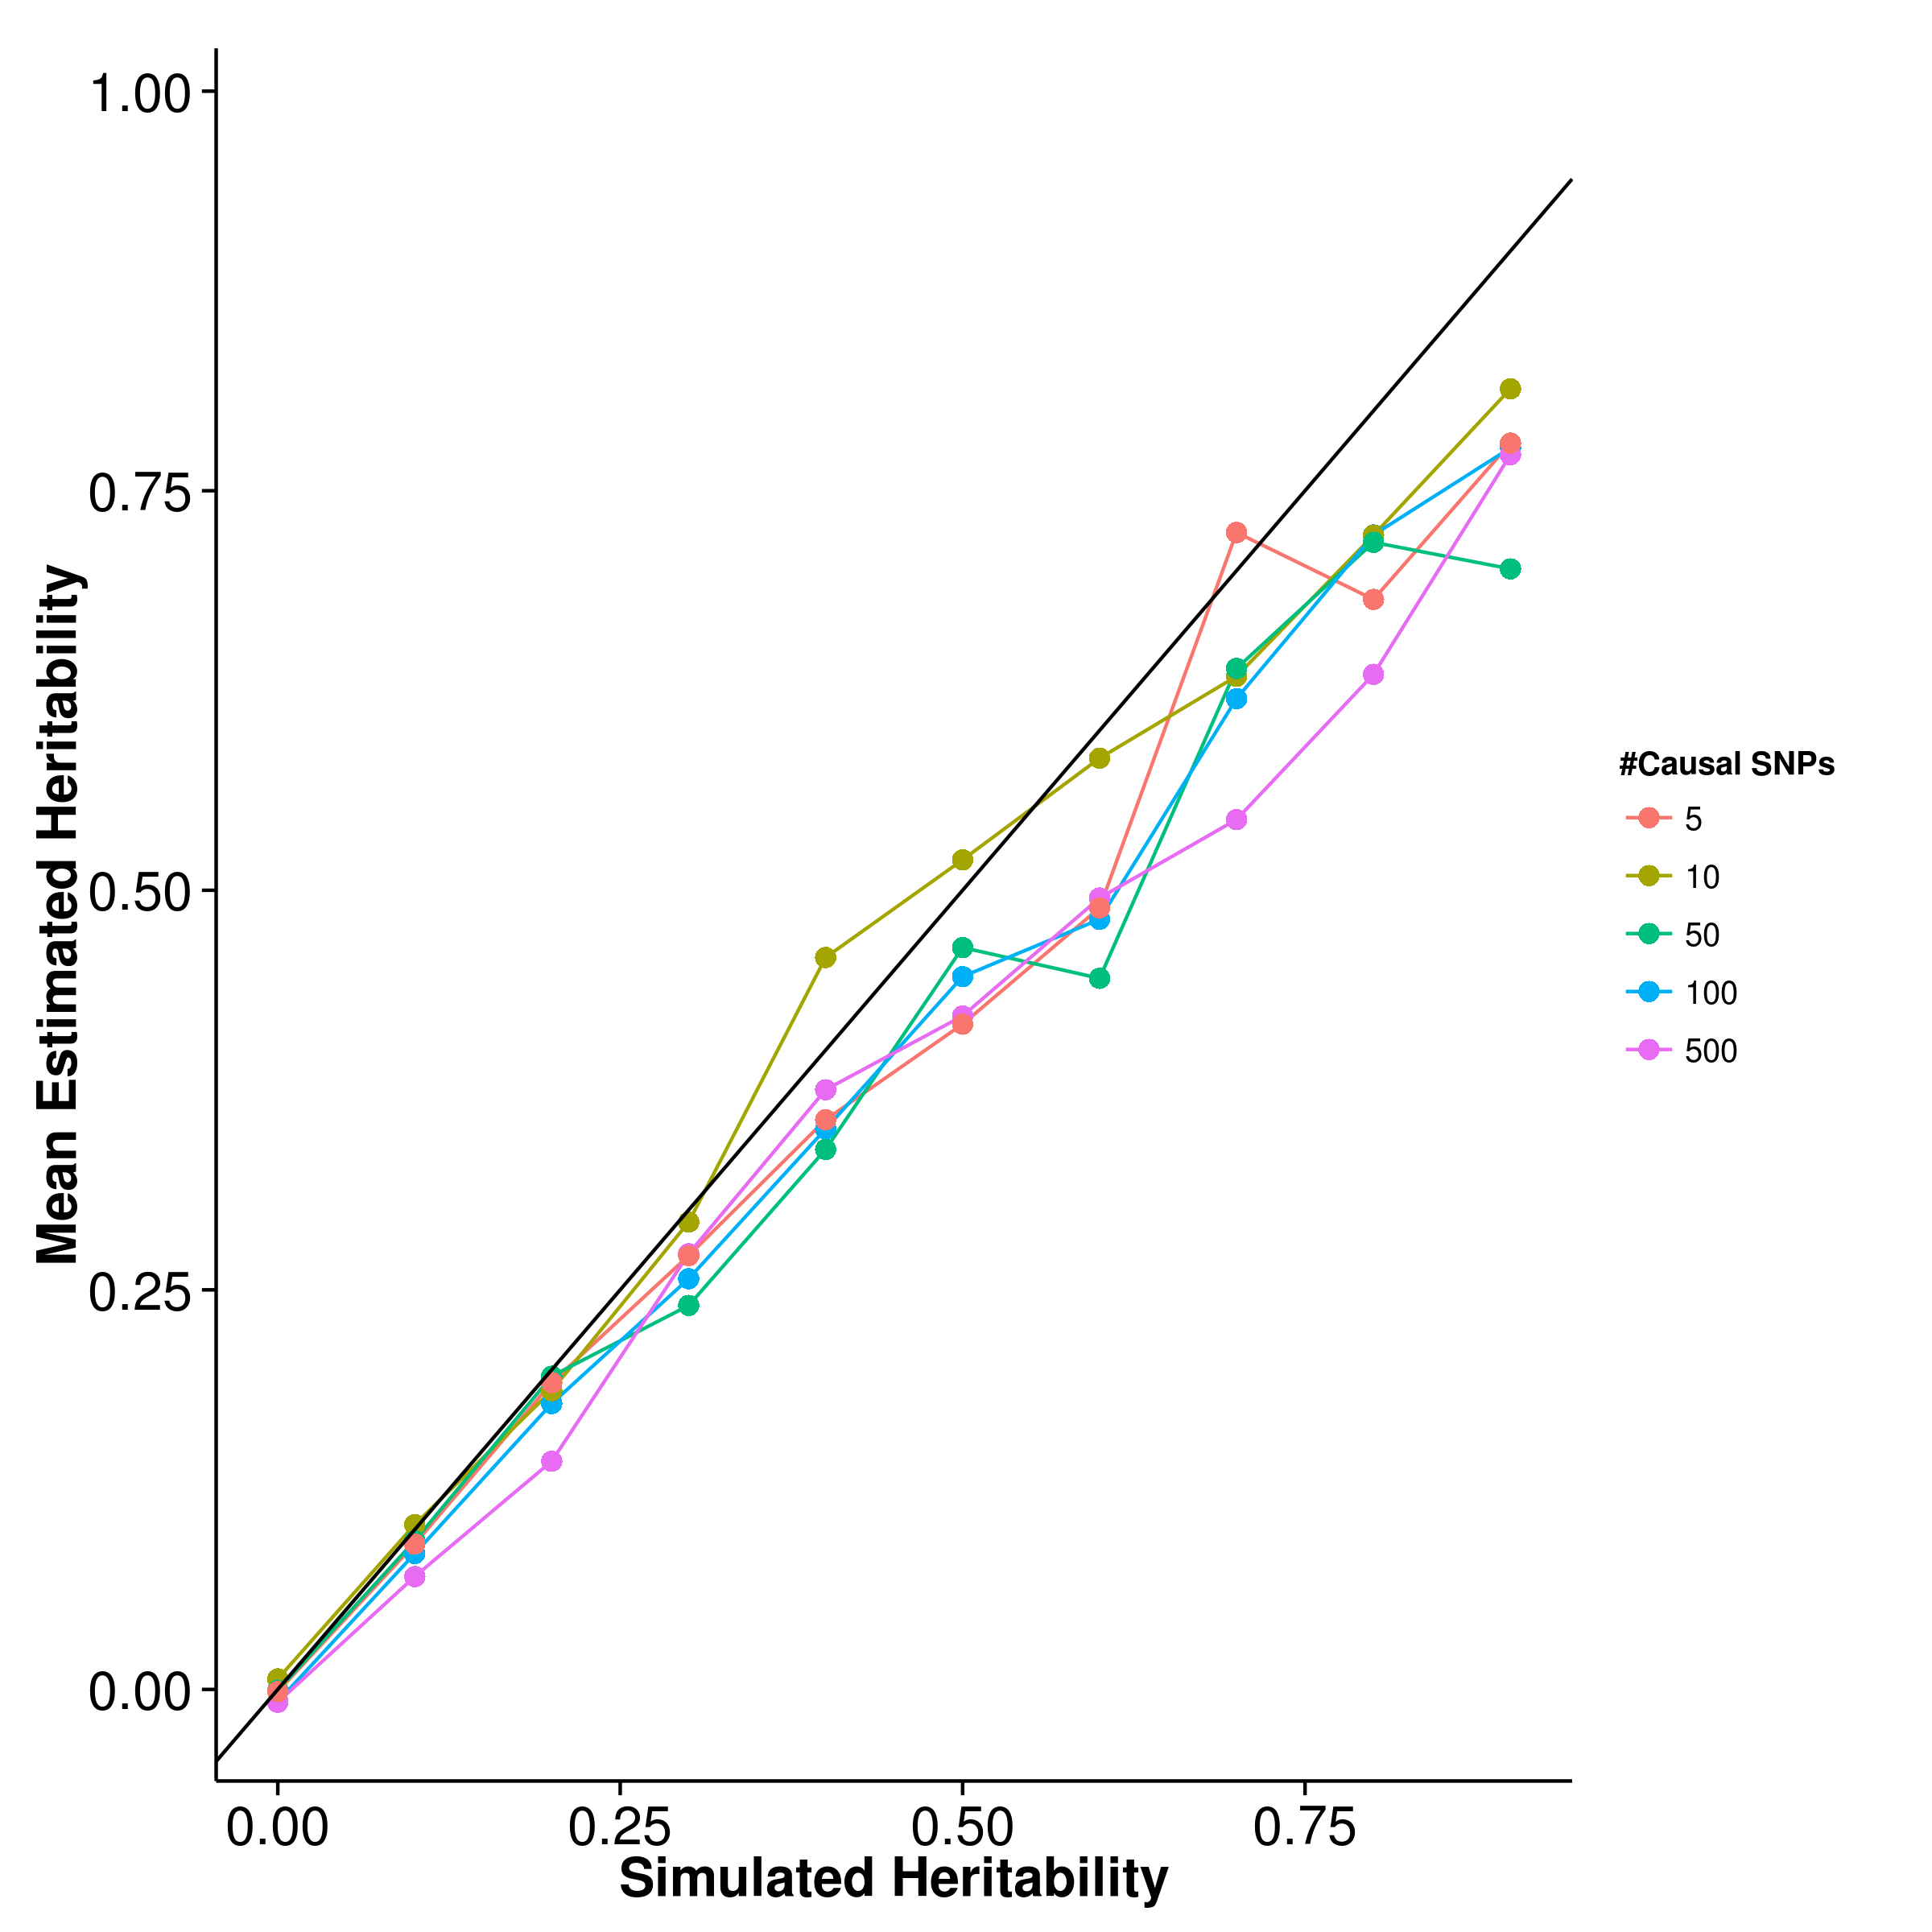
\includegraphics{figure/he_summary/random/ldscIn_Qt_Rand_mean.png}}
				\label{fig:ldscInQtRandMean}
			}
			\caption[Mean of Quantitative Trait Simulation Results]
			{Mean of results from quantitative trait simulation with random effect size simulation.
				Estimations form \gls{shrek} were slightly biased upwards whereas \gls{gcta} and \gls{ldsc} with intercept estimations both biased downwards.
				On the other hand, \gls{ldsc} with fixed intercept provides least biased estimates under polygenic conditions. 
				However, when the number of causal \glspl{SNP} is small (e.g. 5 or 10), an upward bias was observed.} 
			\label{fig:QtRandMean}
		\end{figure}
		
		\begin{figure}
			\centering
			\subfloat[SHREK]{
				\scalebox{.4}{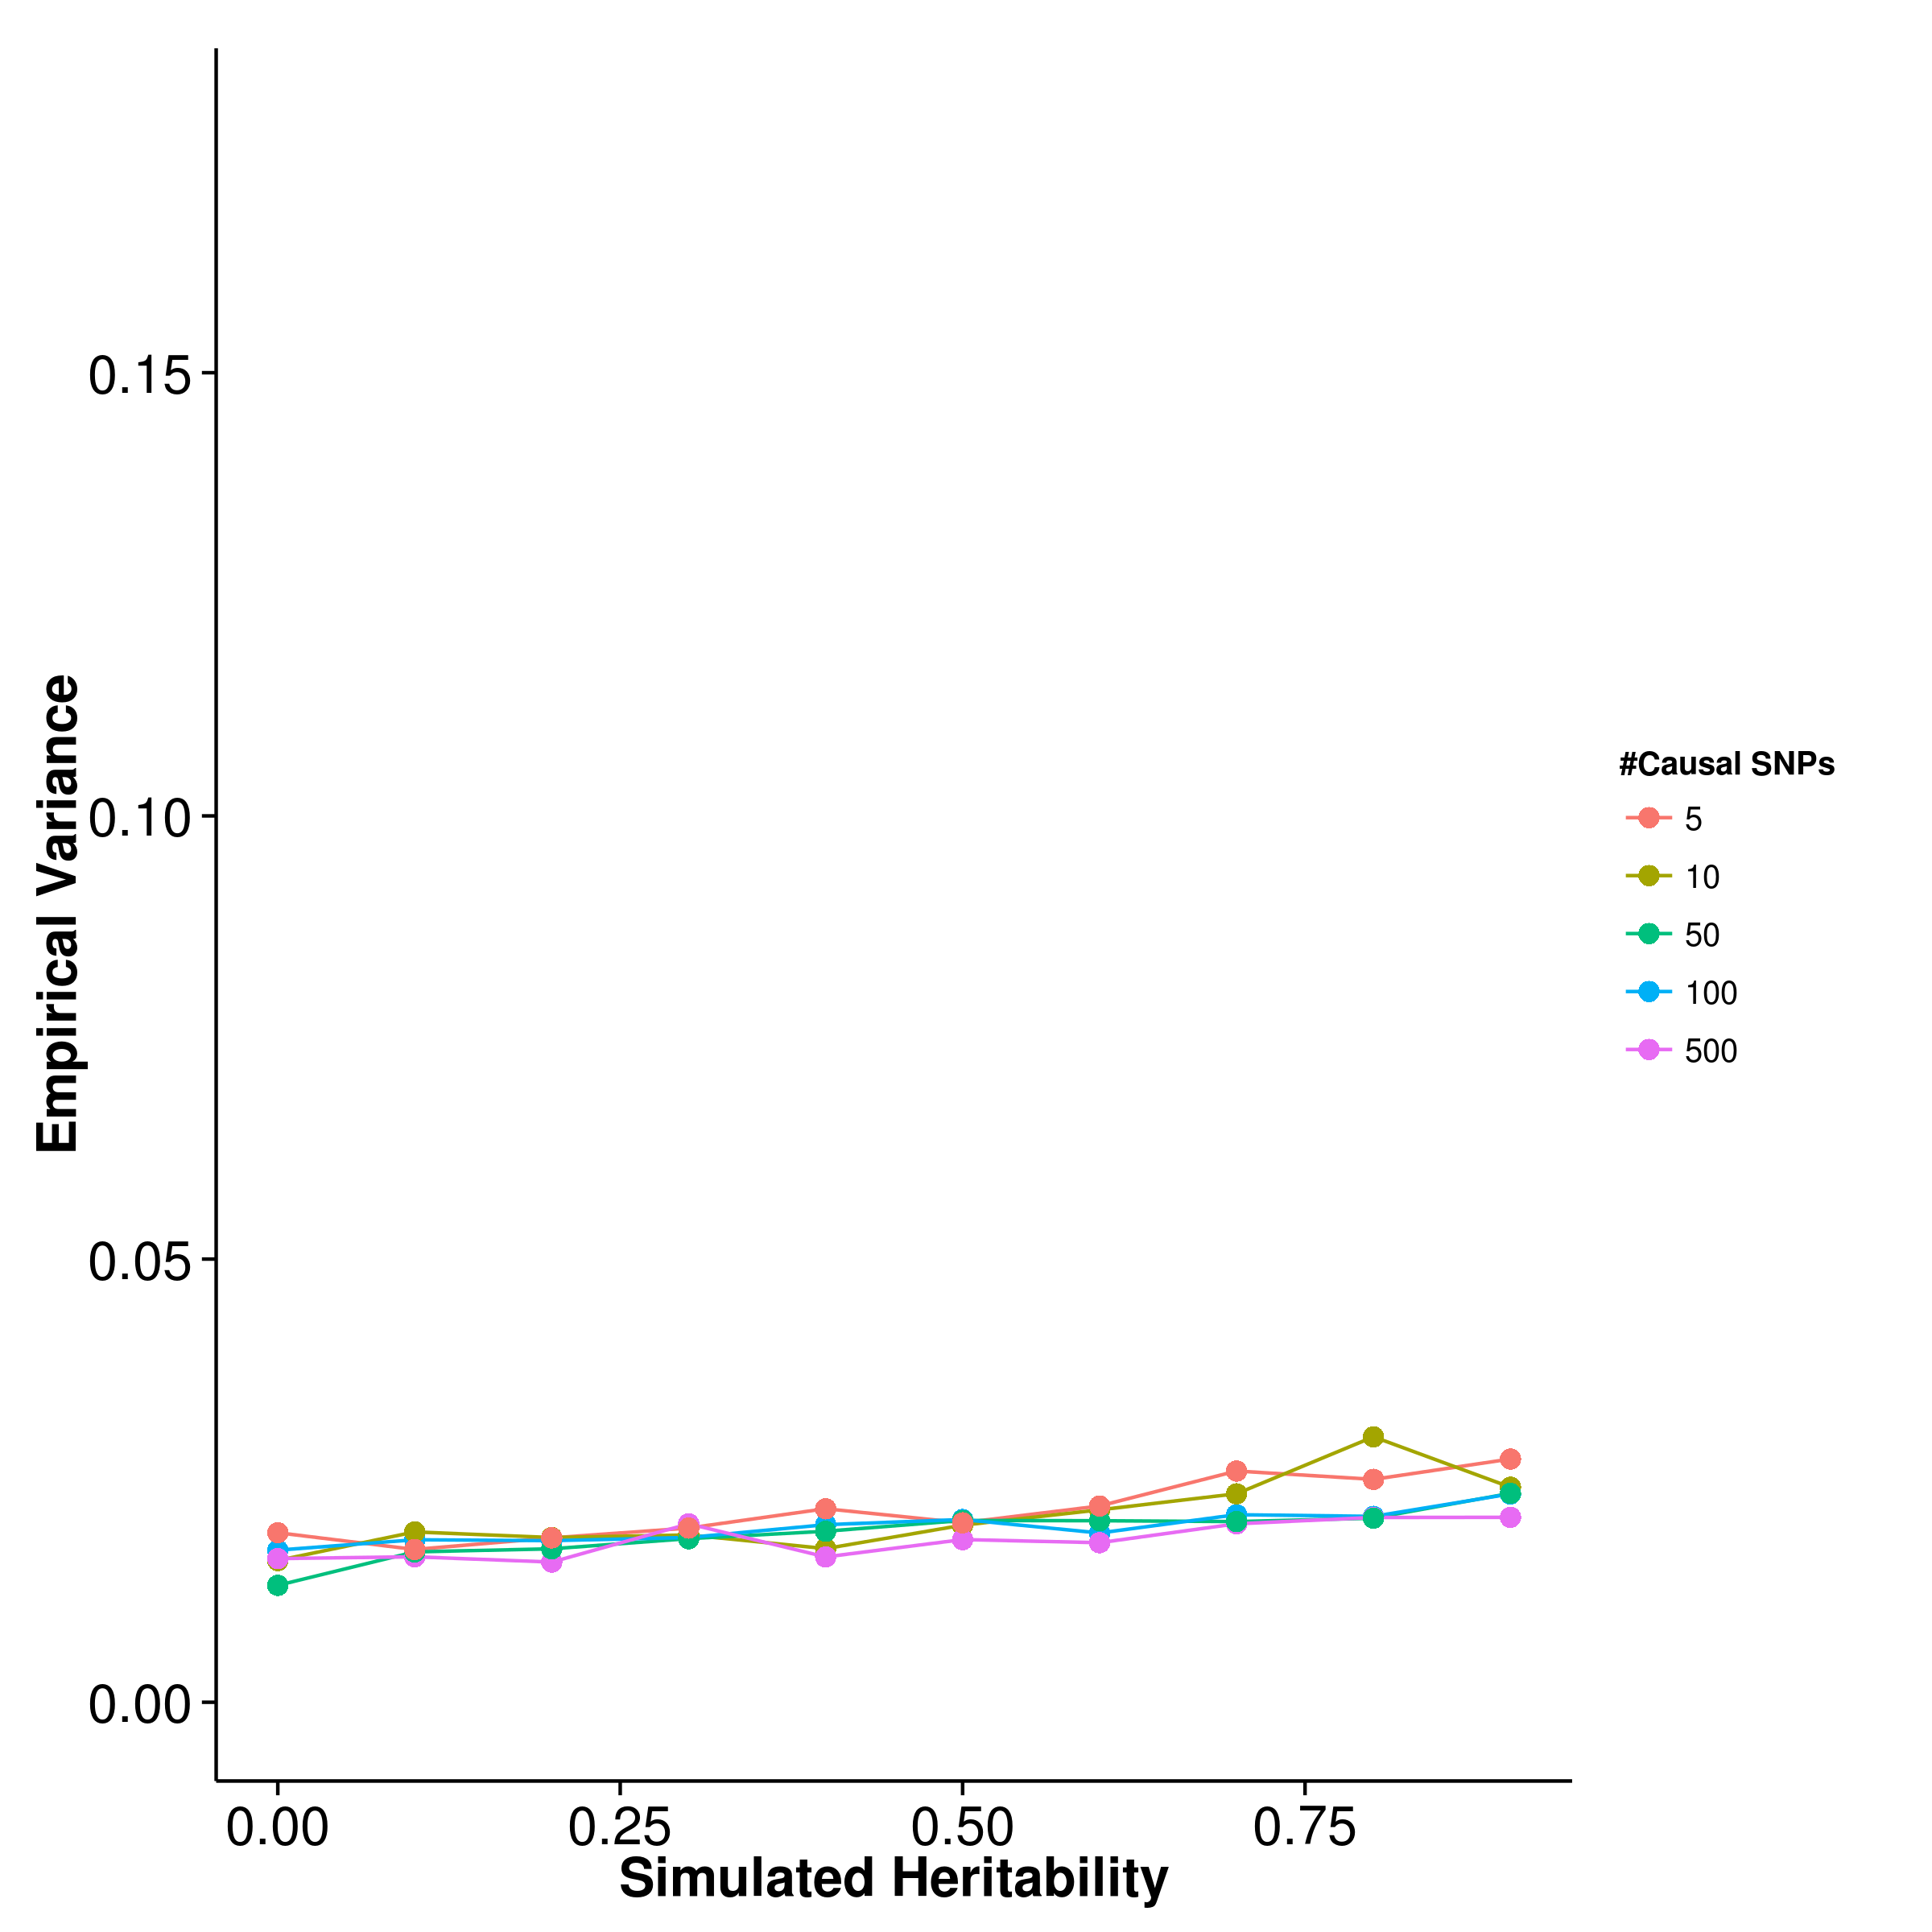
\includegraphics{figure/he_summary/random/shrek_Qt_Rand_sd.png}}
				\label{fig:shrekQtRandVar}
			}
			\subfloat[GCTA]{
				\scalebox{.4}{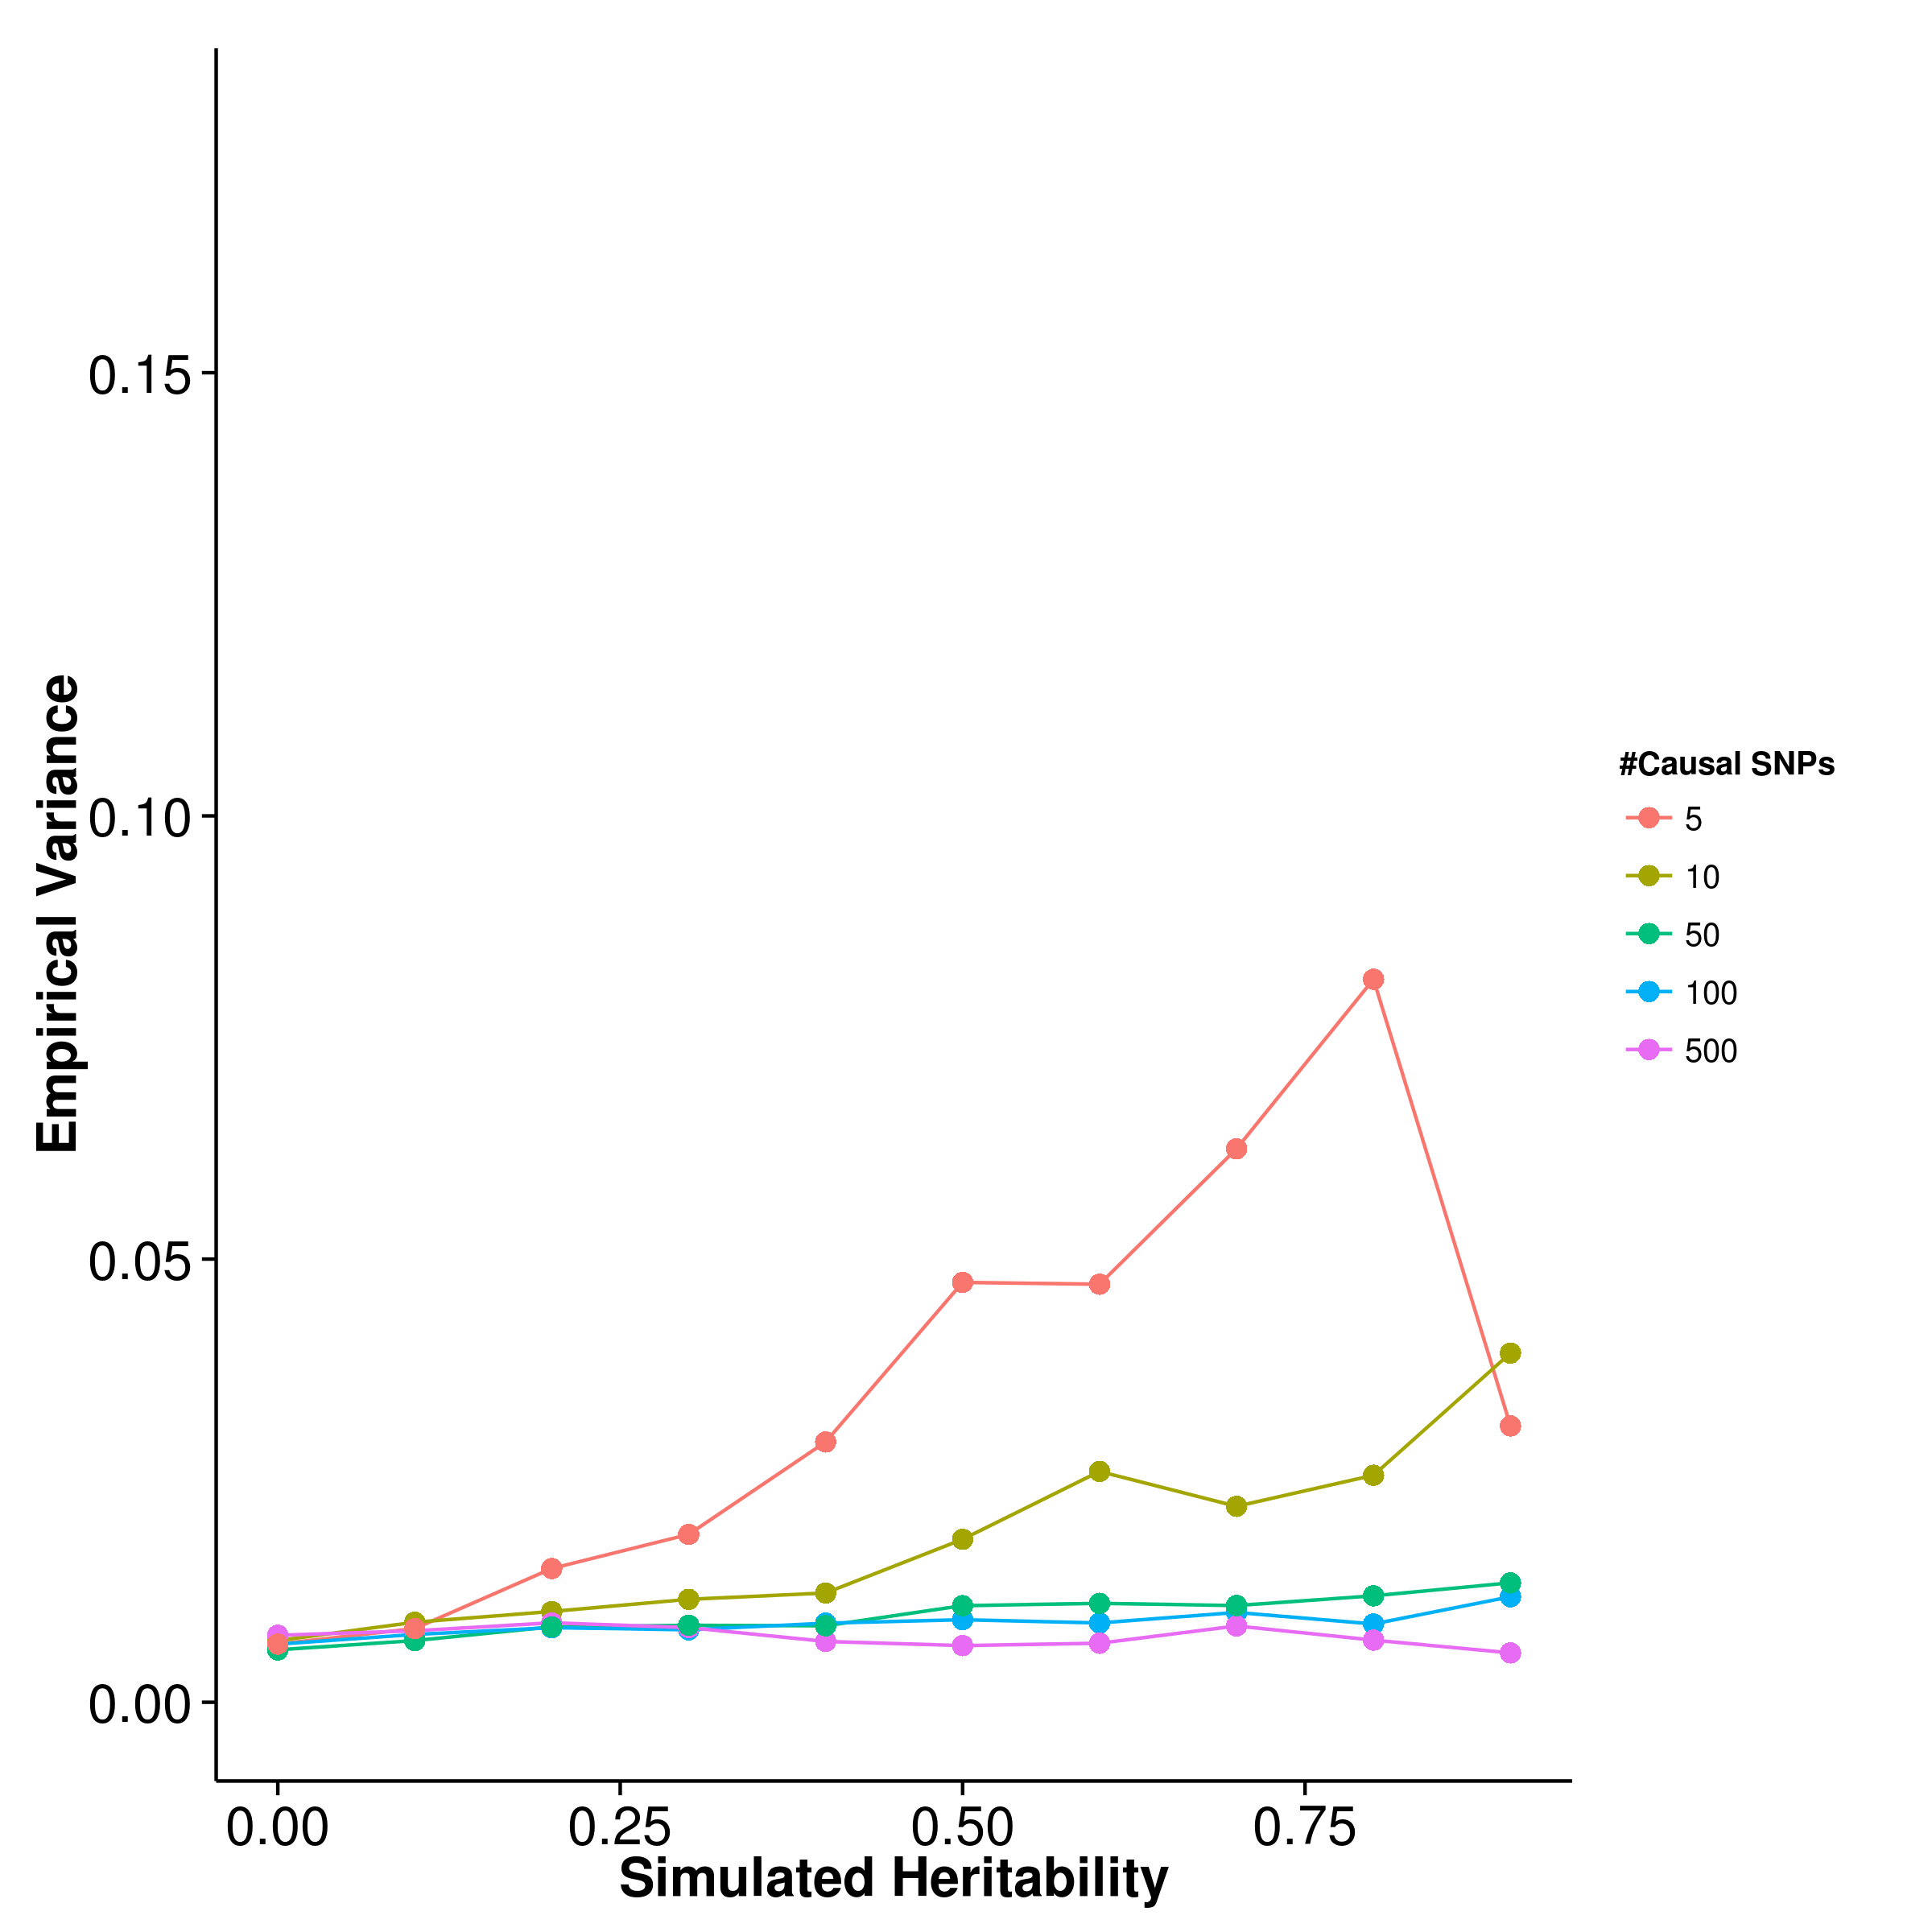
\includegraphics{figure/he_summary/random/gcta_Qt_Rand_sd.png}}
				\label{fig:gctaQtRandVar}
			}\\
			\subfloat[LDSC with fix intercept]{
				\scalebox{.4}{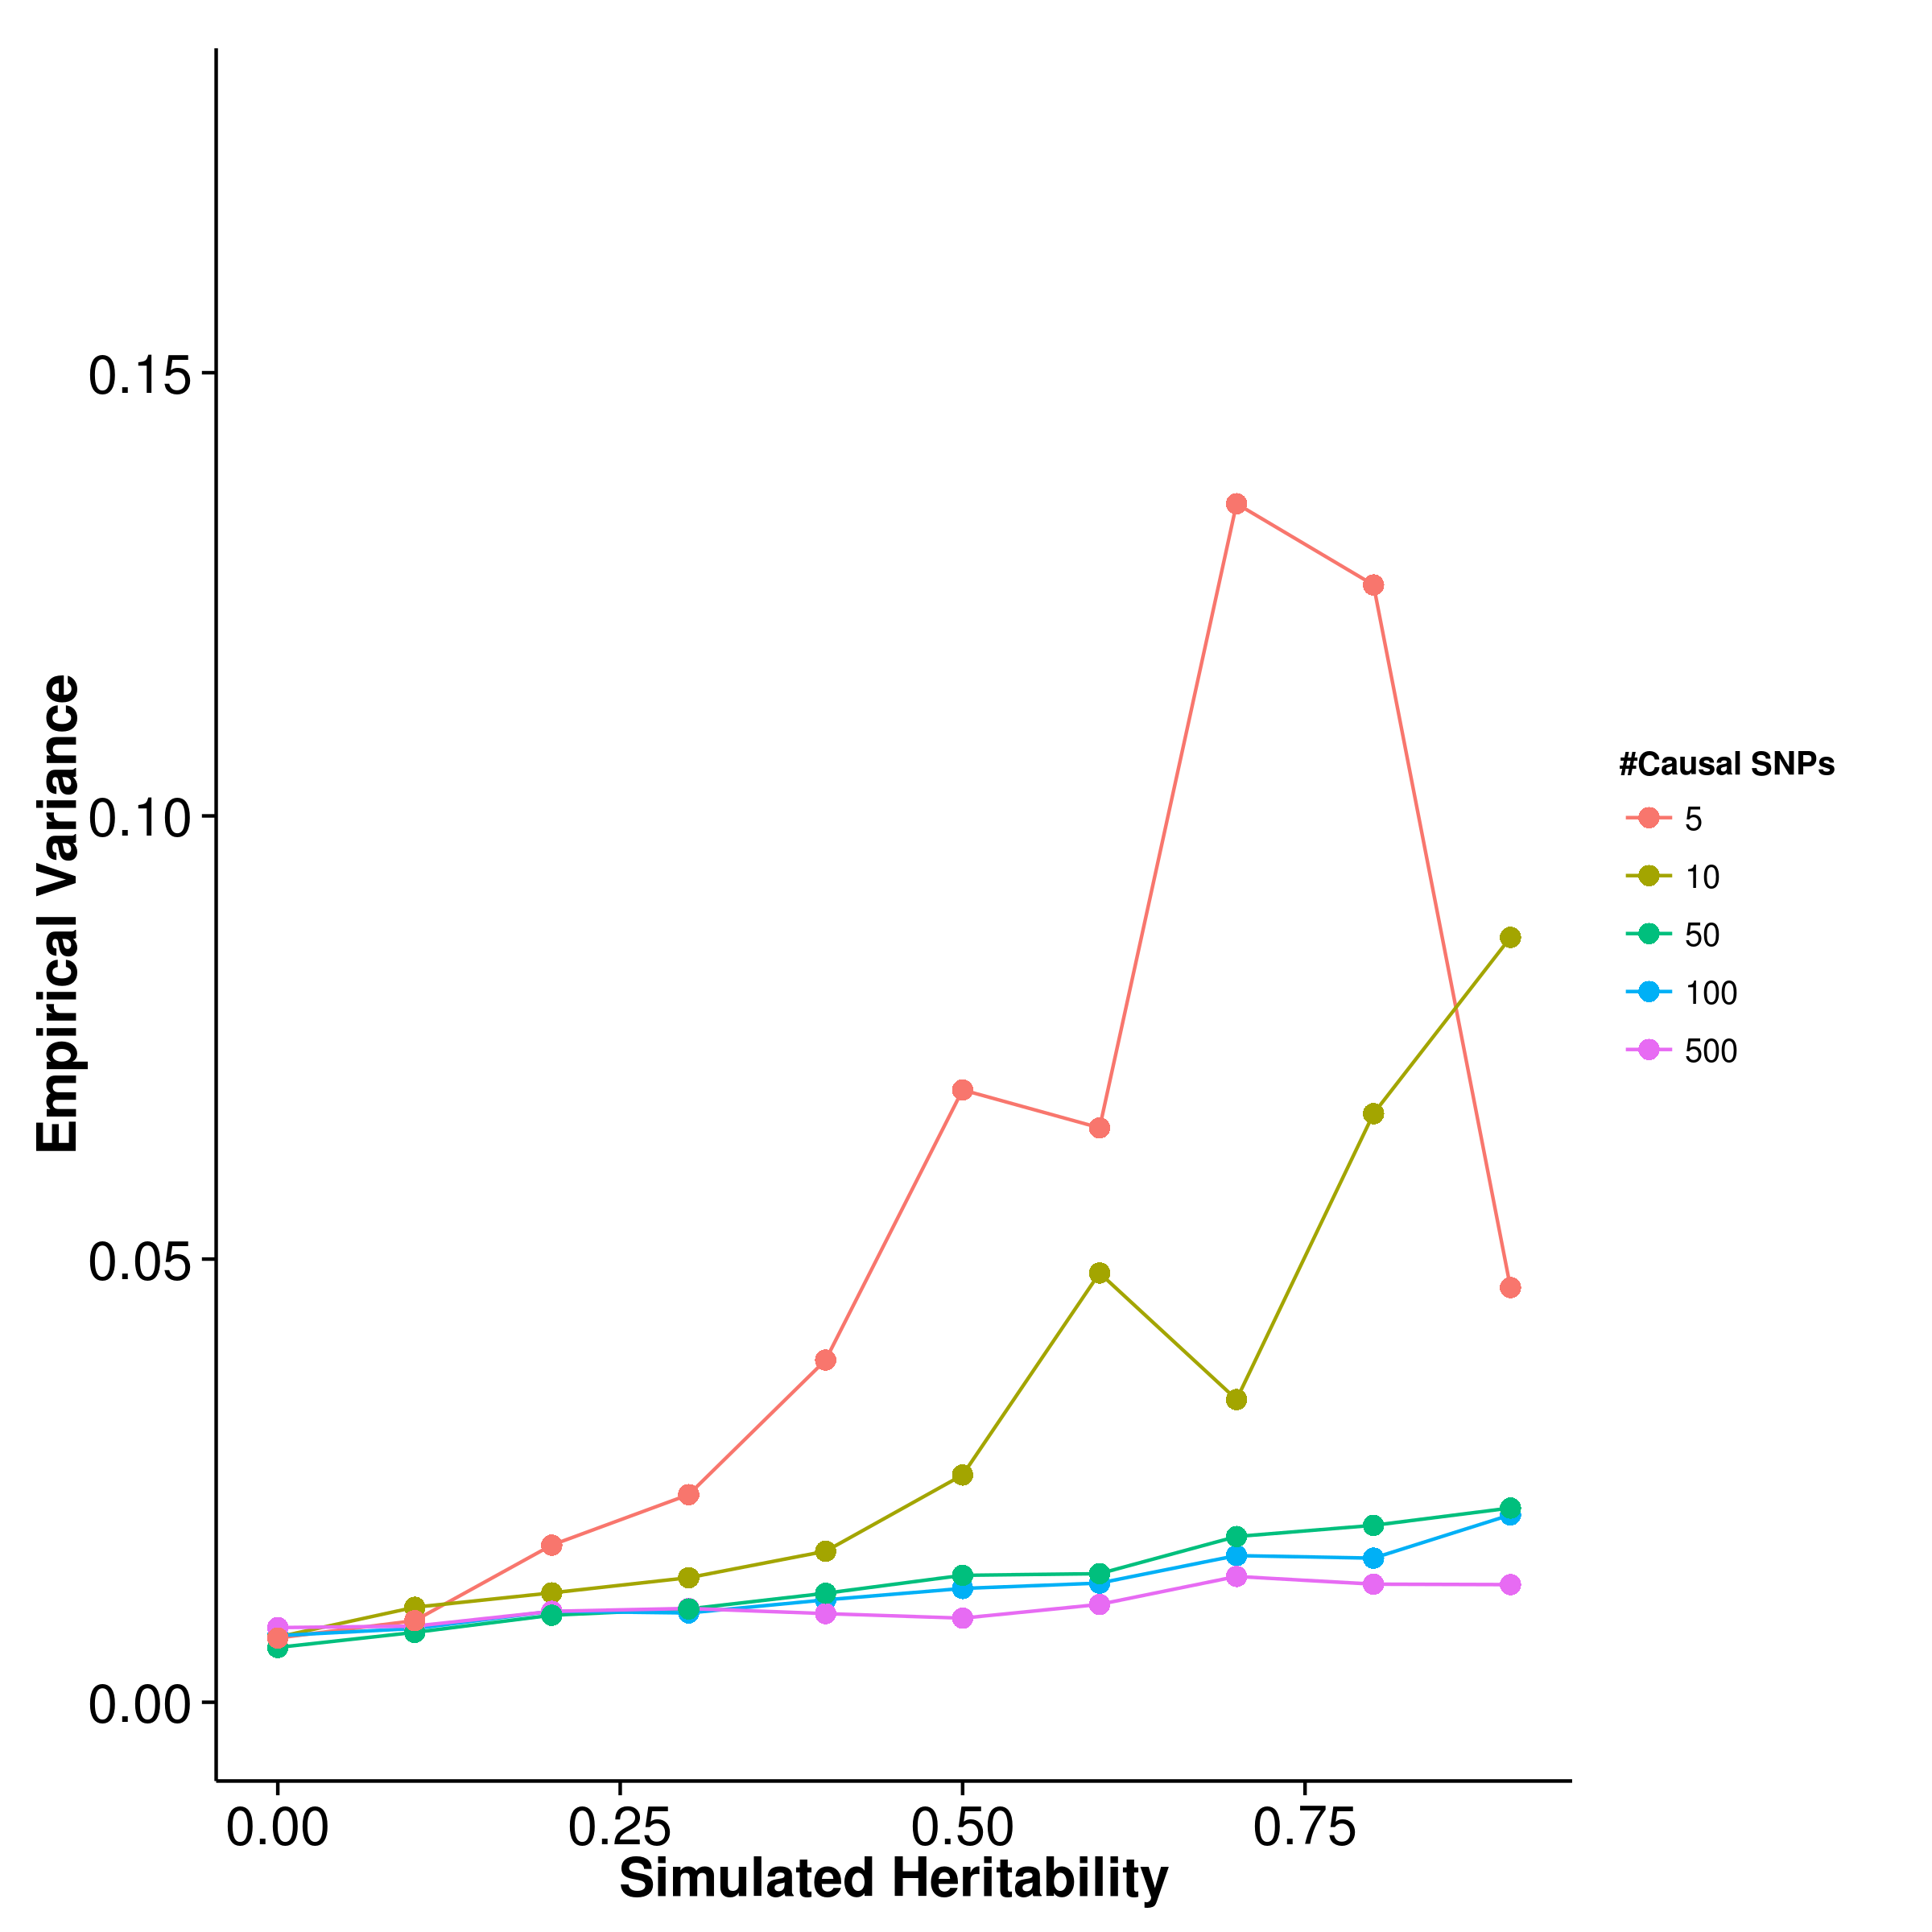
\includegraphics{figure/he_summary/random/ldsc_Qt_Rand_sd.png}}
				\label{fig:ldscQtRandVar}
			}
			\subfloat[LDSC with intercept estimation]{
				
				\scalebox{.4}{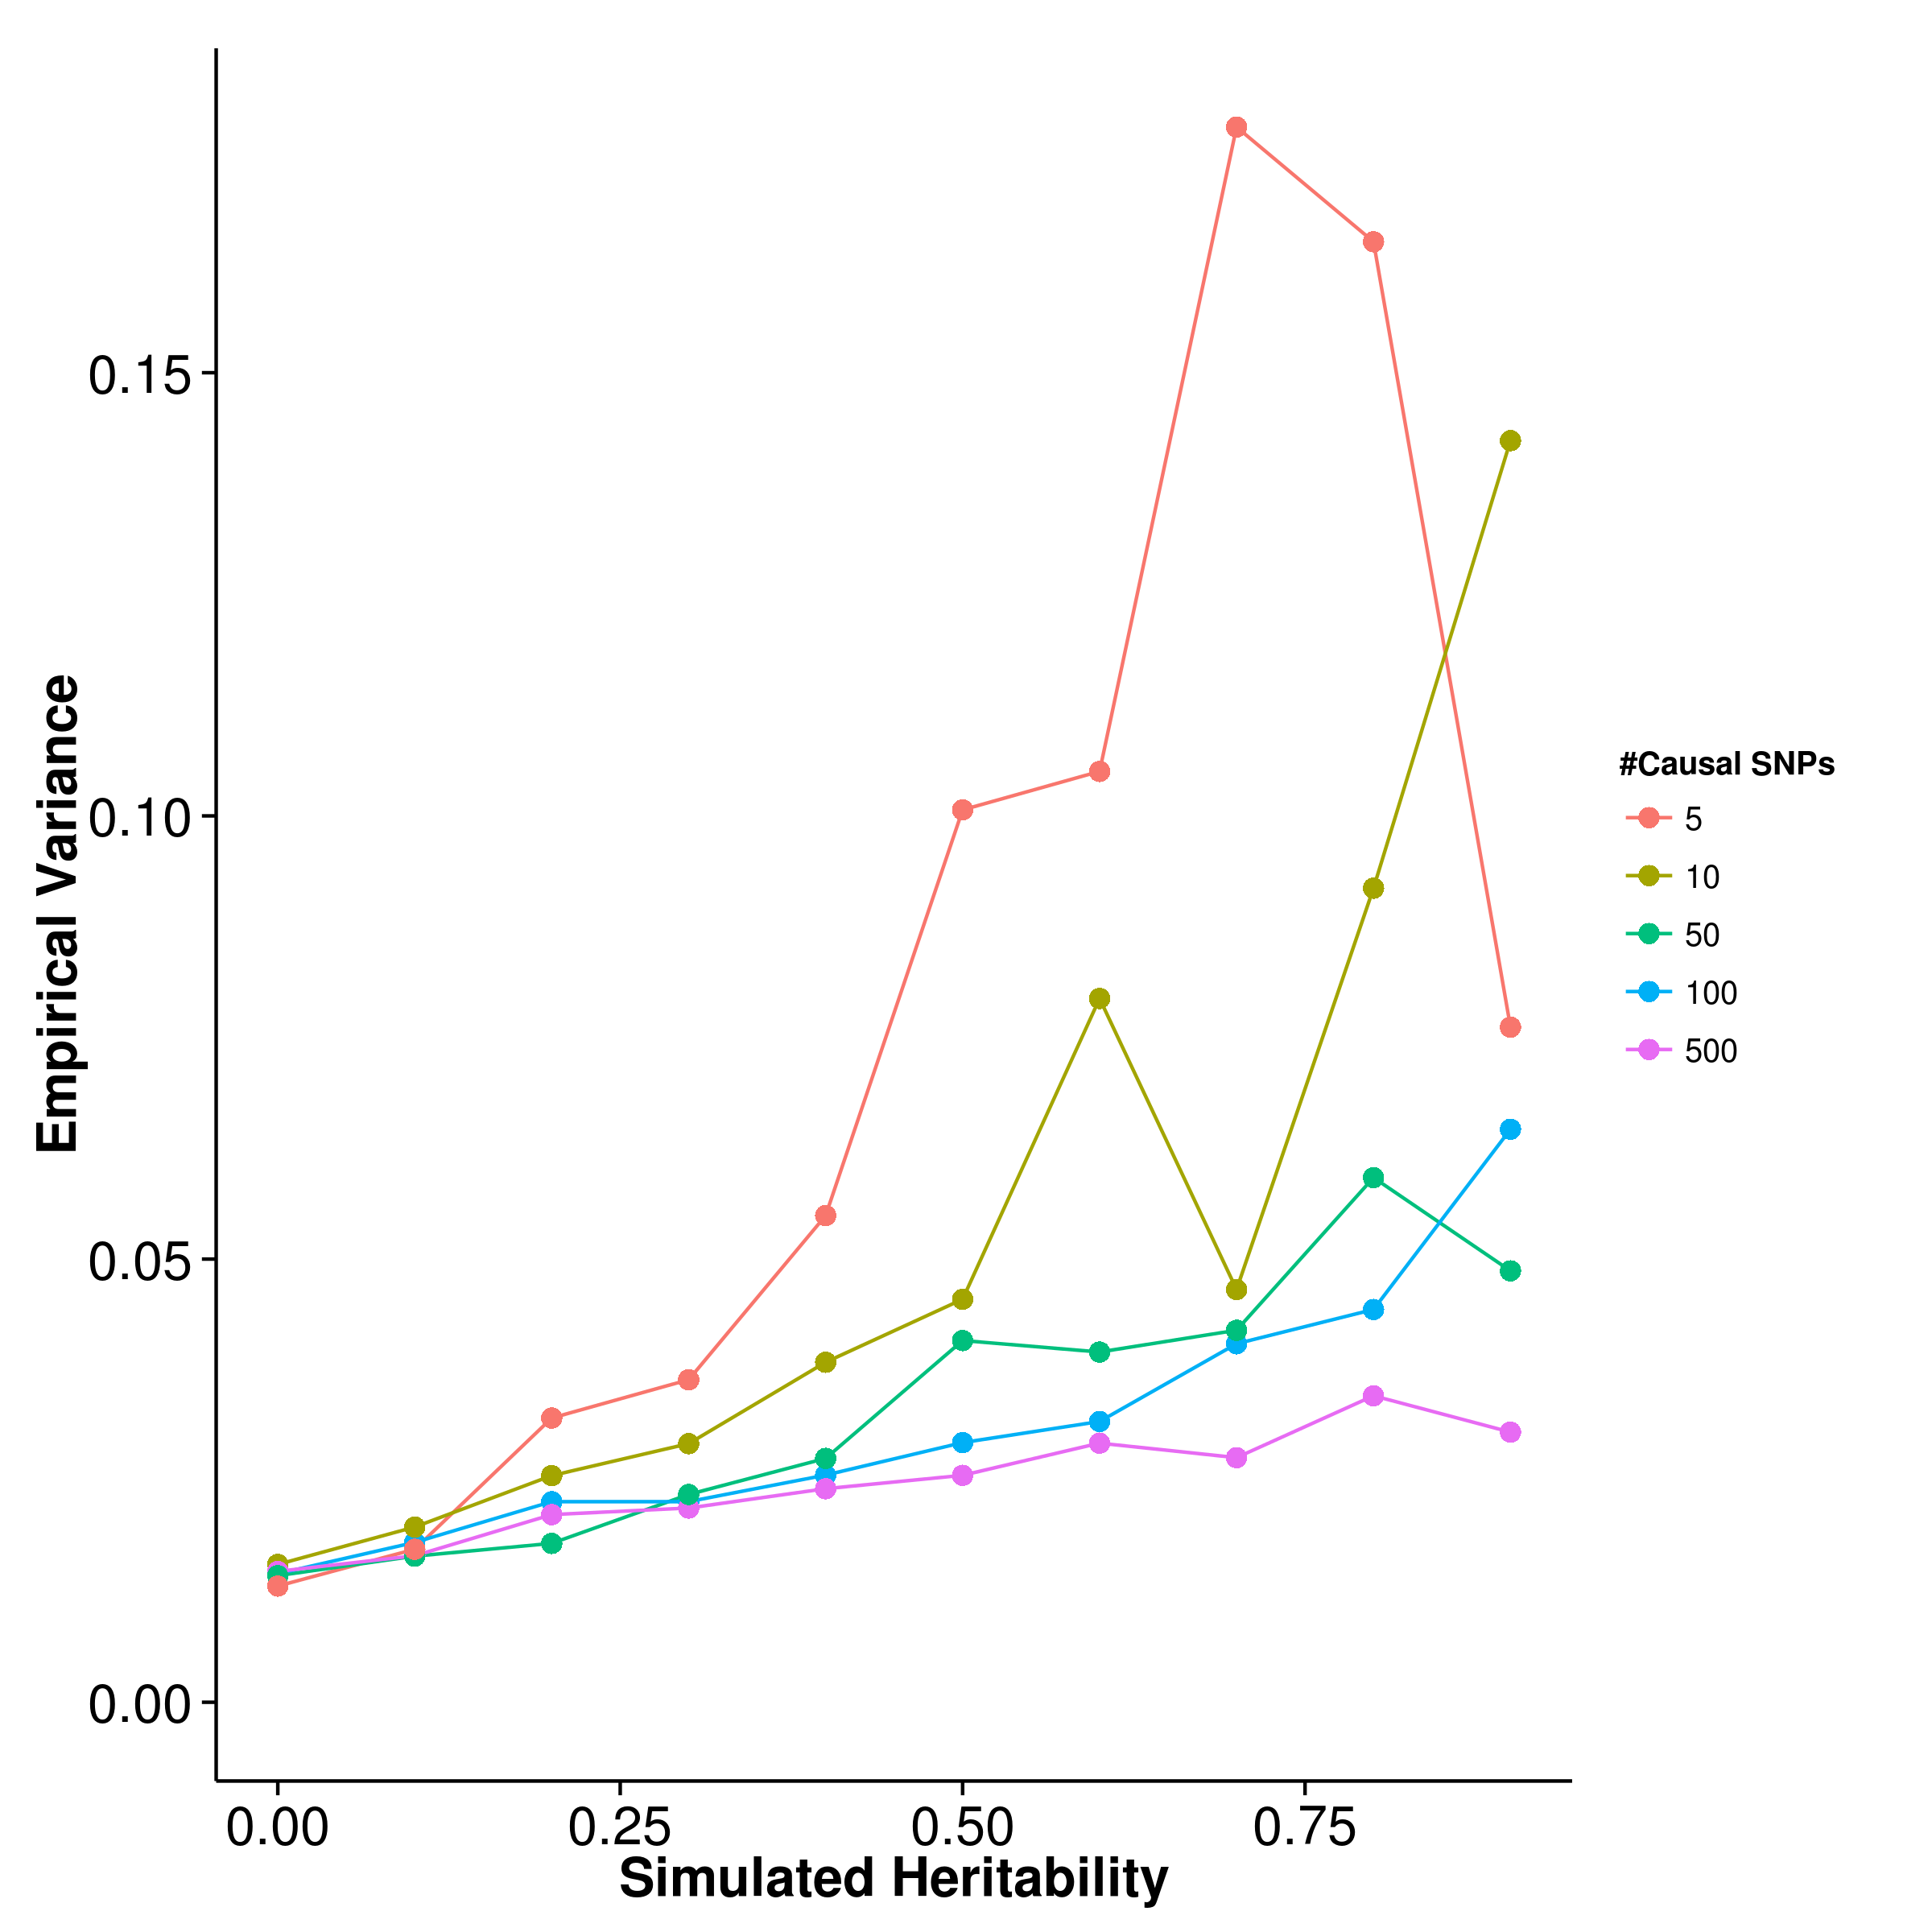
\includegraphics{figure/he_summary/random/ldscIn_Qt_Rand_sd.png}}
				\label{fig:ldscInQtRandVar}
			}
			\caption[Variance of Quantitative Trait Simulation Results]
			{Variance of results from quantitative trait simulation with random effect size simulation.
				Under the polygenic conditions, \gls{gcta} has the smallest variance, follow by \gls{ldsc}. 
				However, it was observed when the number of causal \glspl{SNP} decreases, the variance of the estimation increases for all algorithm, with variance of the \gls{shrek} estimate being the least affected.
				In fact, under oligogenic conditions, \gls{shrek} has a lower empirical variance when compared to \gls{ldsc}.
			} 
			\label{fig:QtRandVar}
		\end{figure}
		
		\begin{figure}
			\centering
			\subfloat[SHREK]{
				\scalebox{.4}{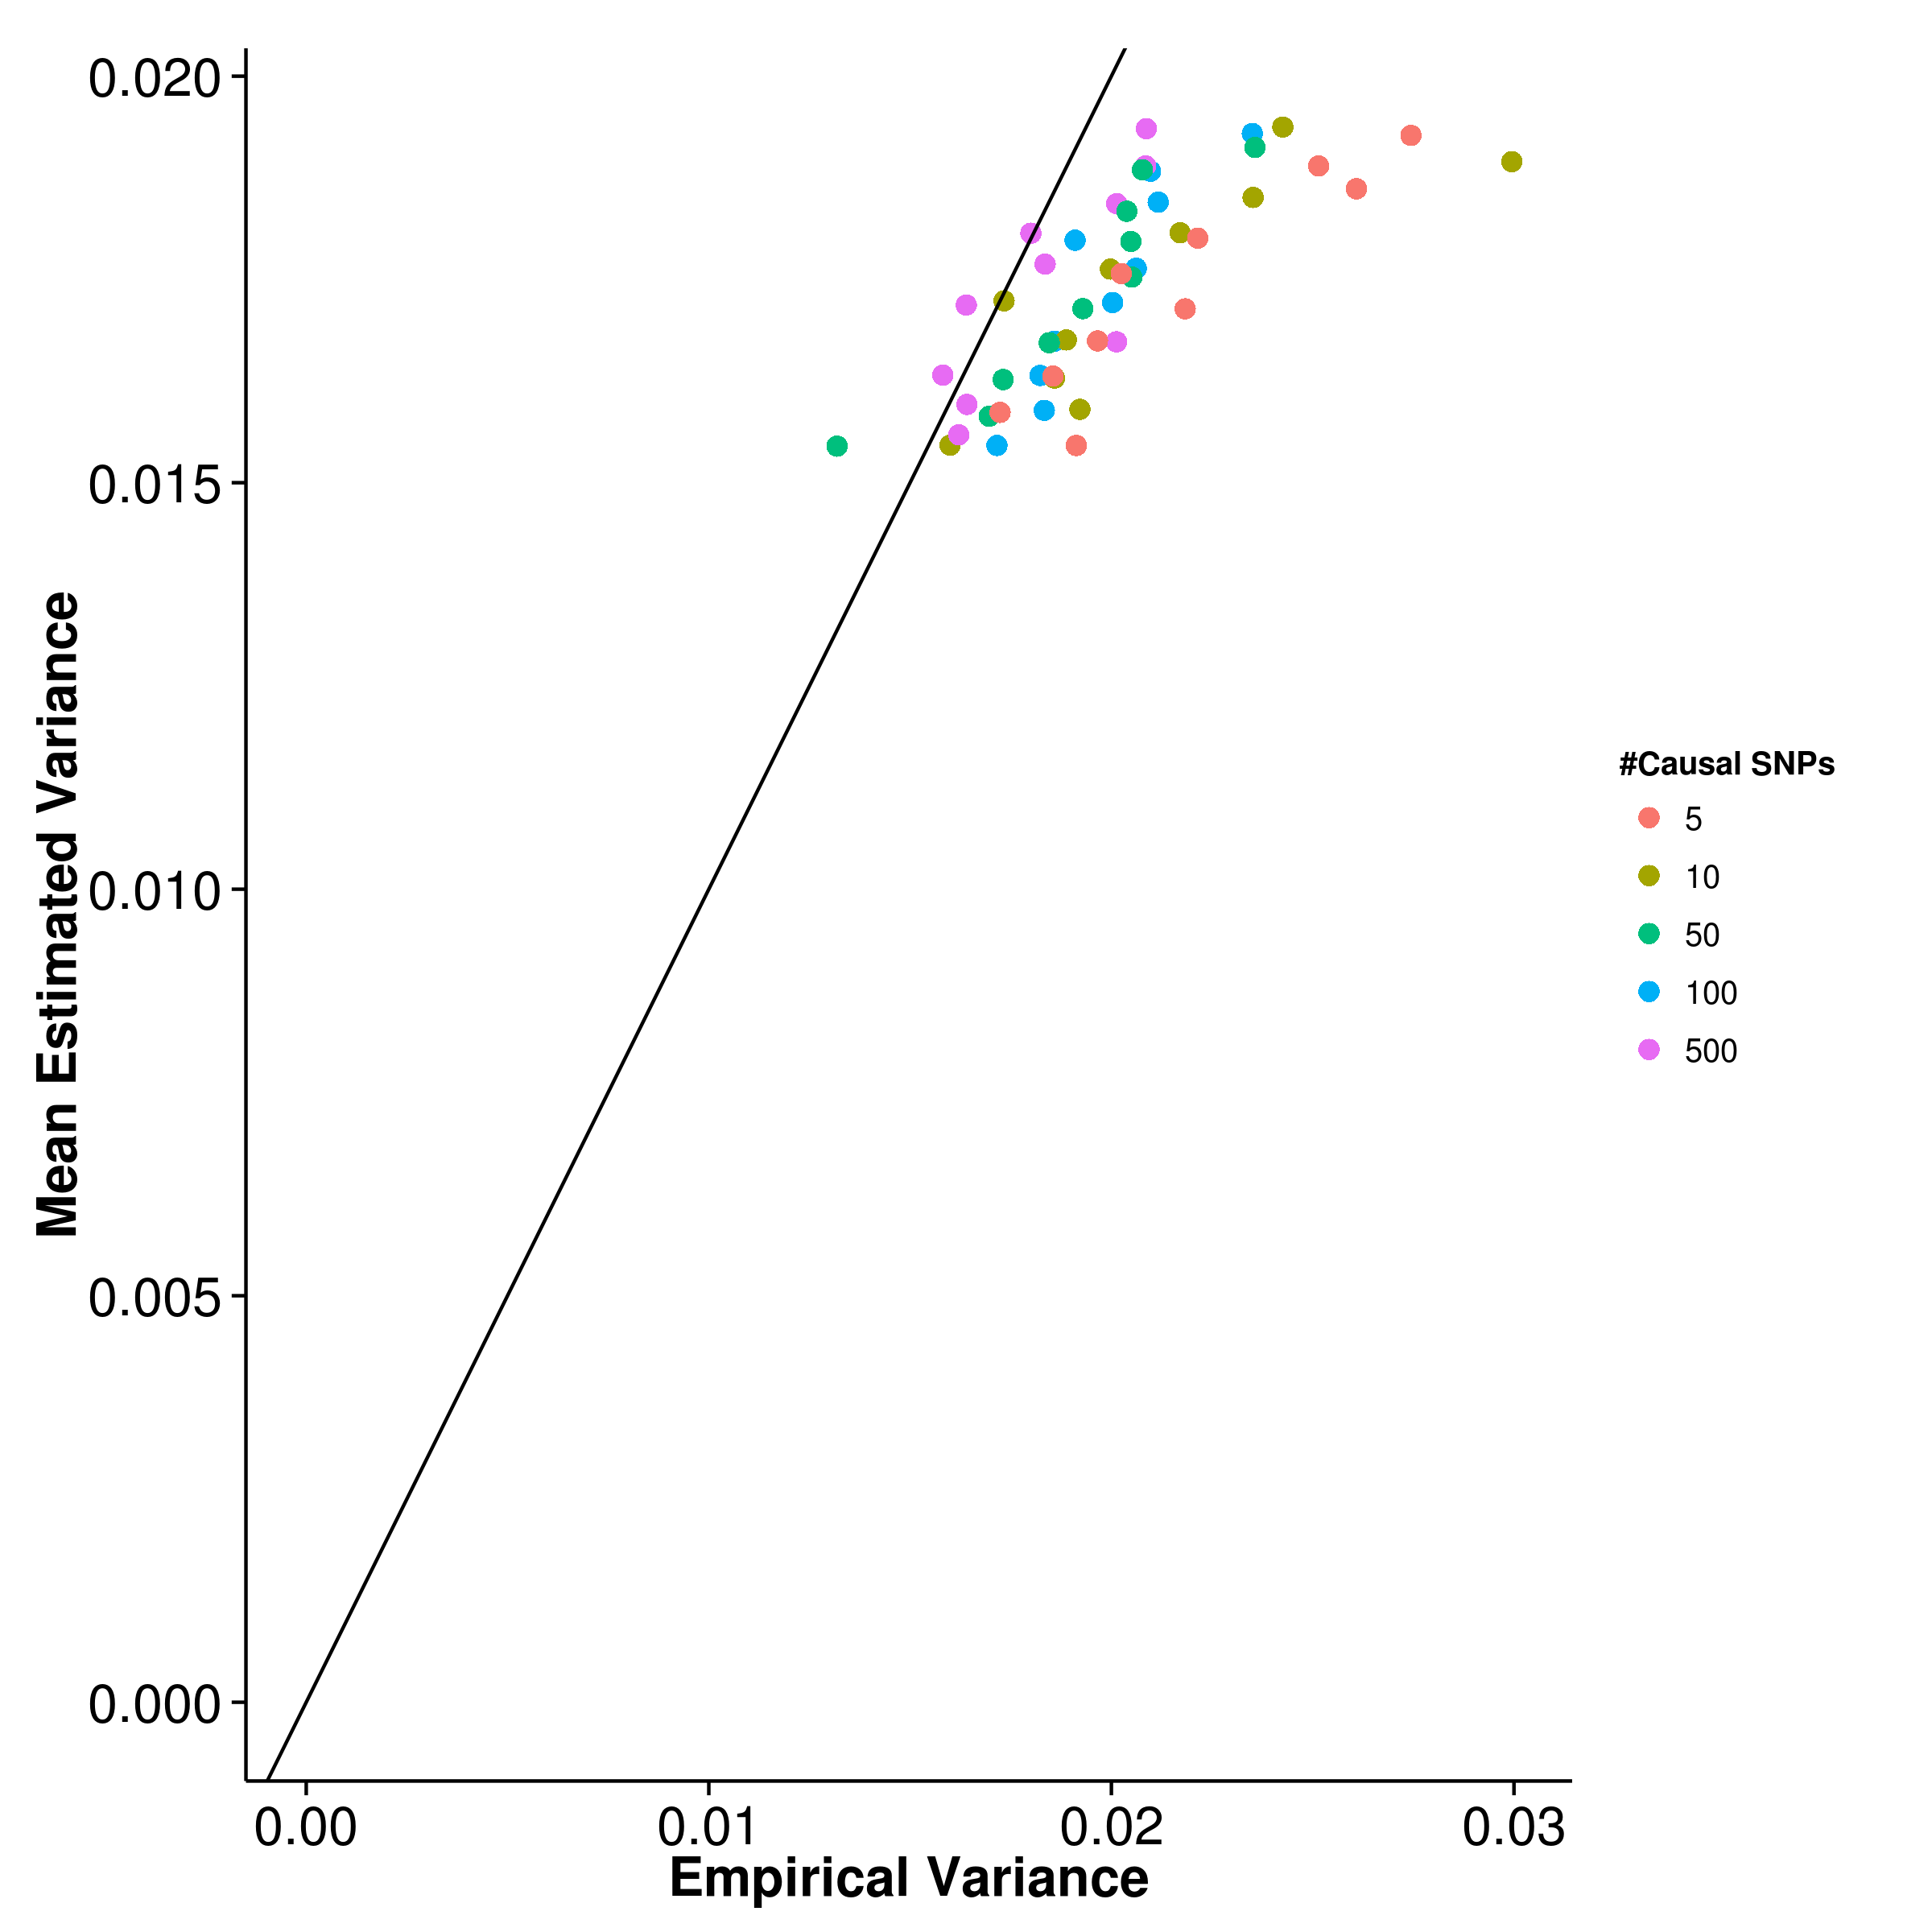
\includegraphics{figure/he_summary/random/shrek_Qt_Rand_sdCom.png}}
				\label{fig:shrekQtRandVarCom}
			}
			\subfloat[GCTA]{
				\scalebox{.4}{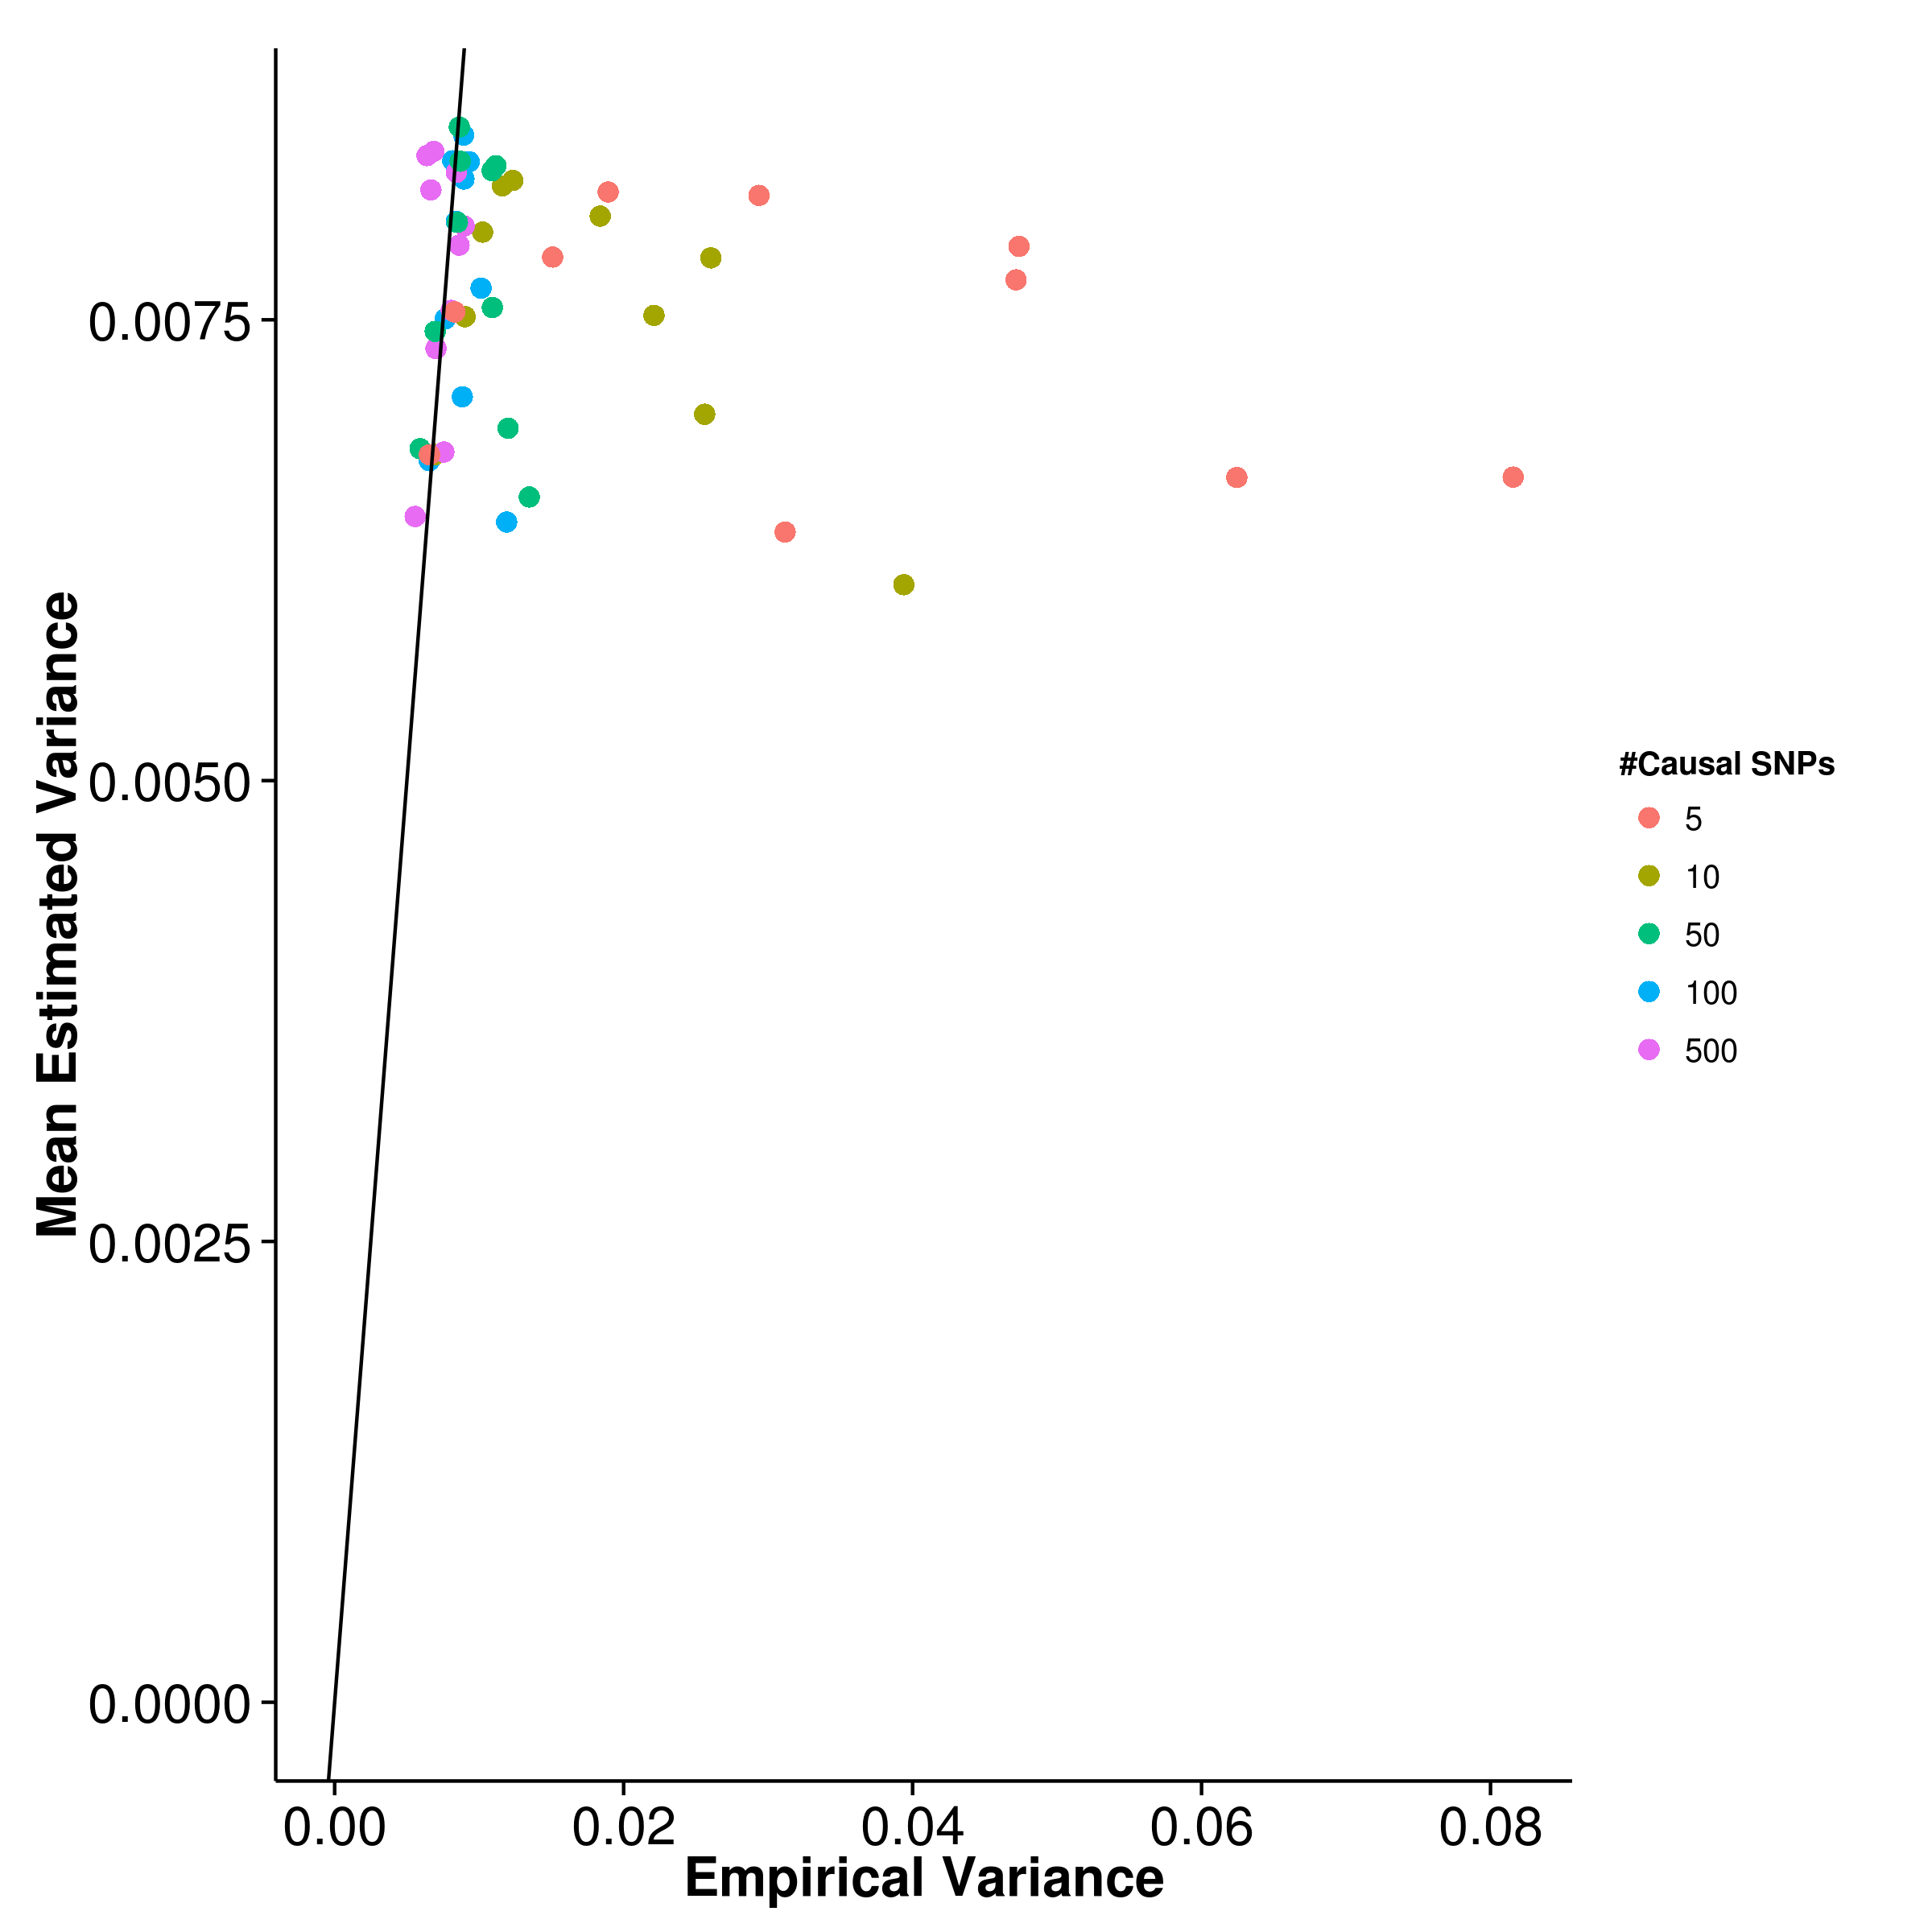
\includegraphics{figure/he_summary/random/gcta_Qt_Rand_sdCom.png}}
				\label{fig:gctaQtRandVarCom}
			}\\
			\subfloat[LDSC with fix intercept]{
				\scalebox{.4}{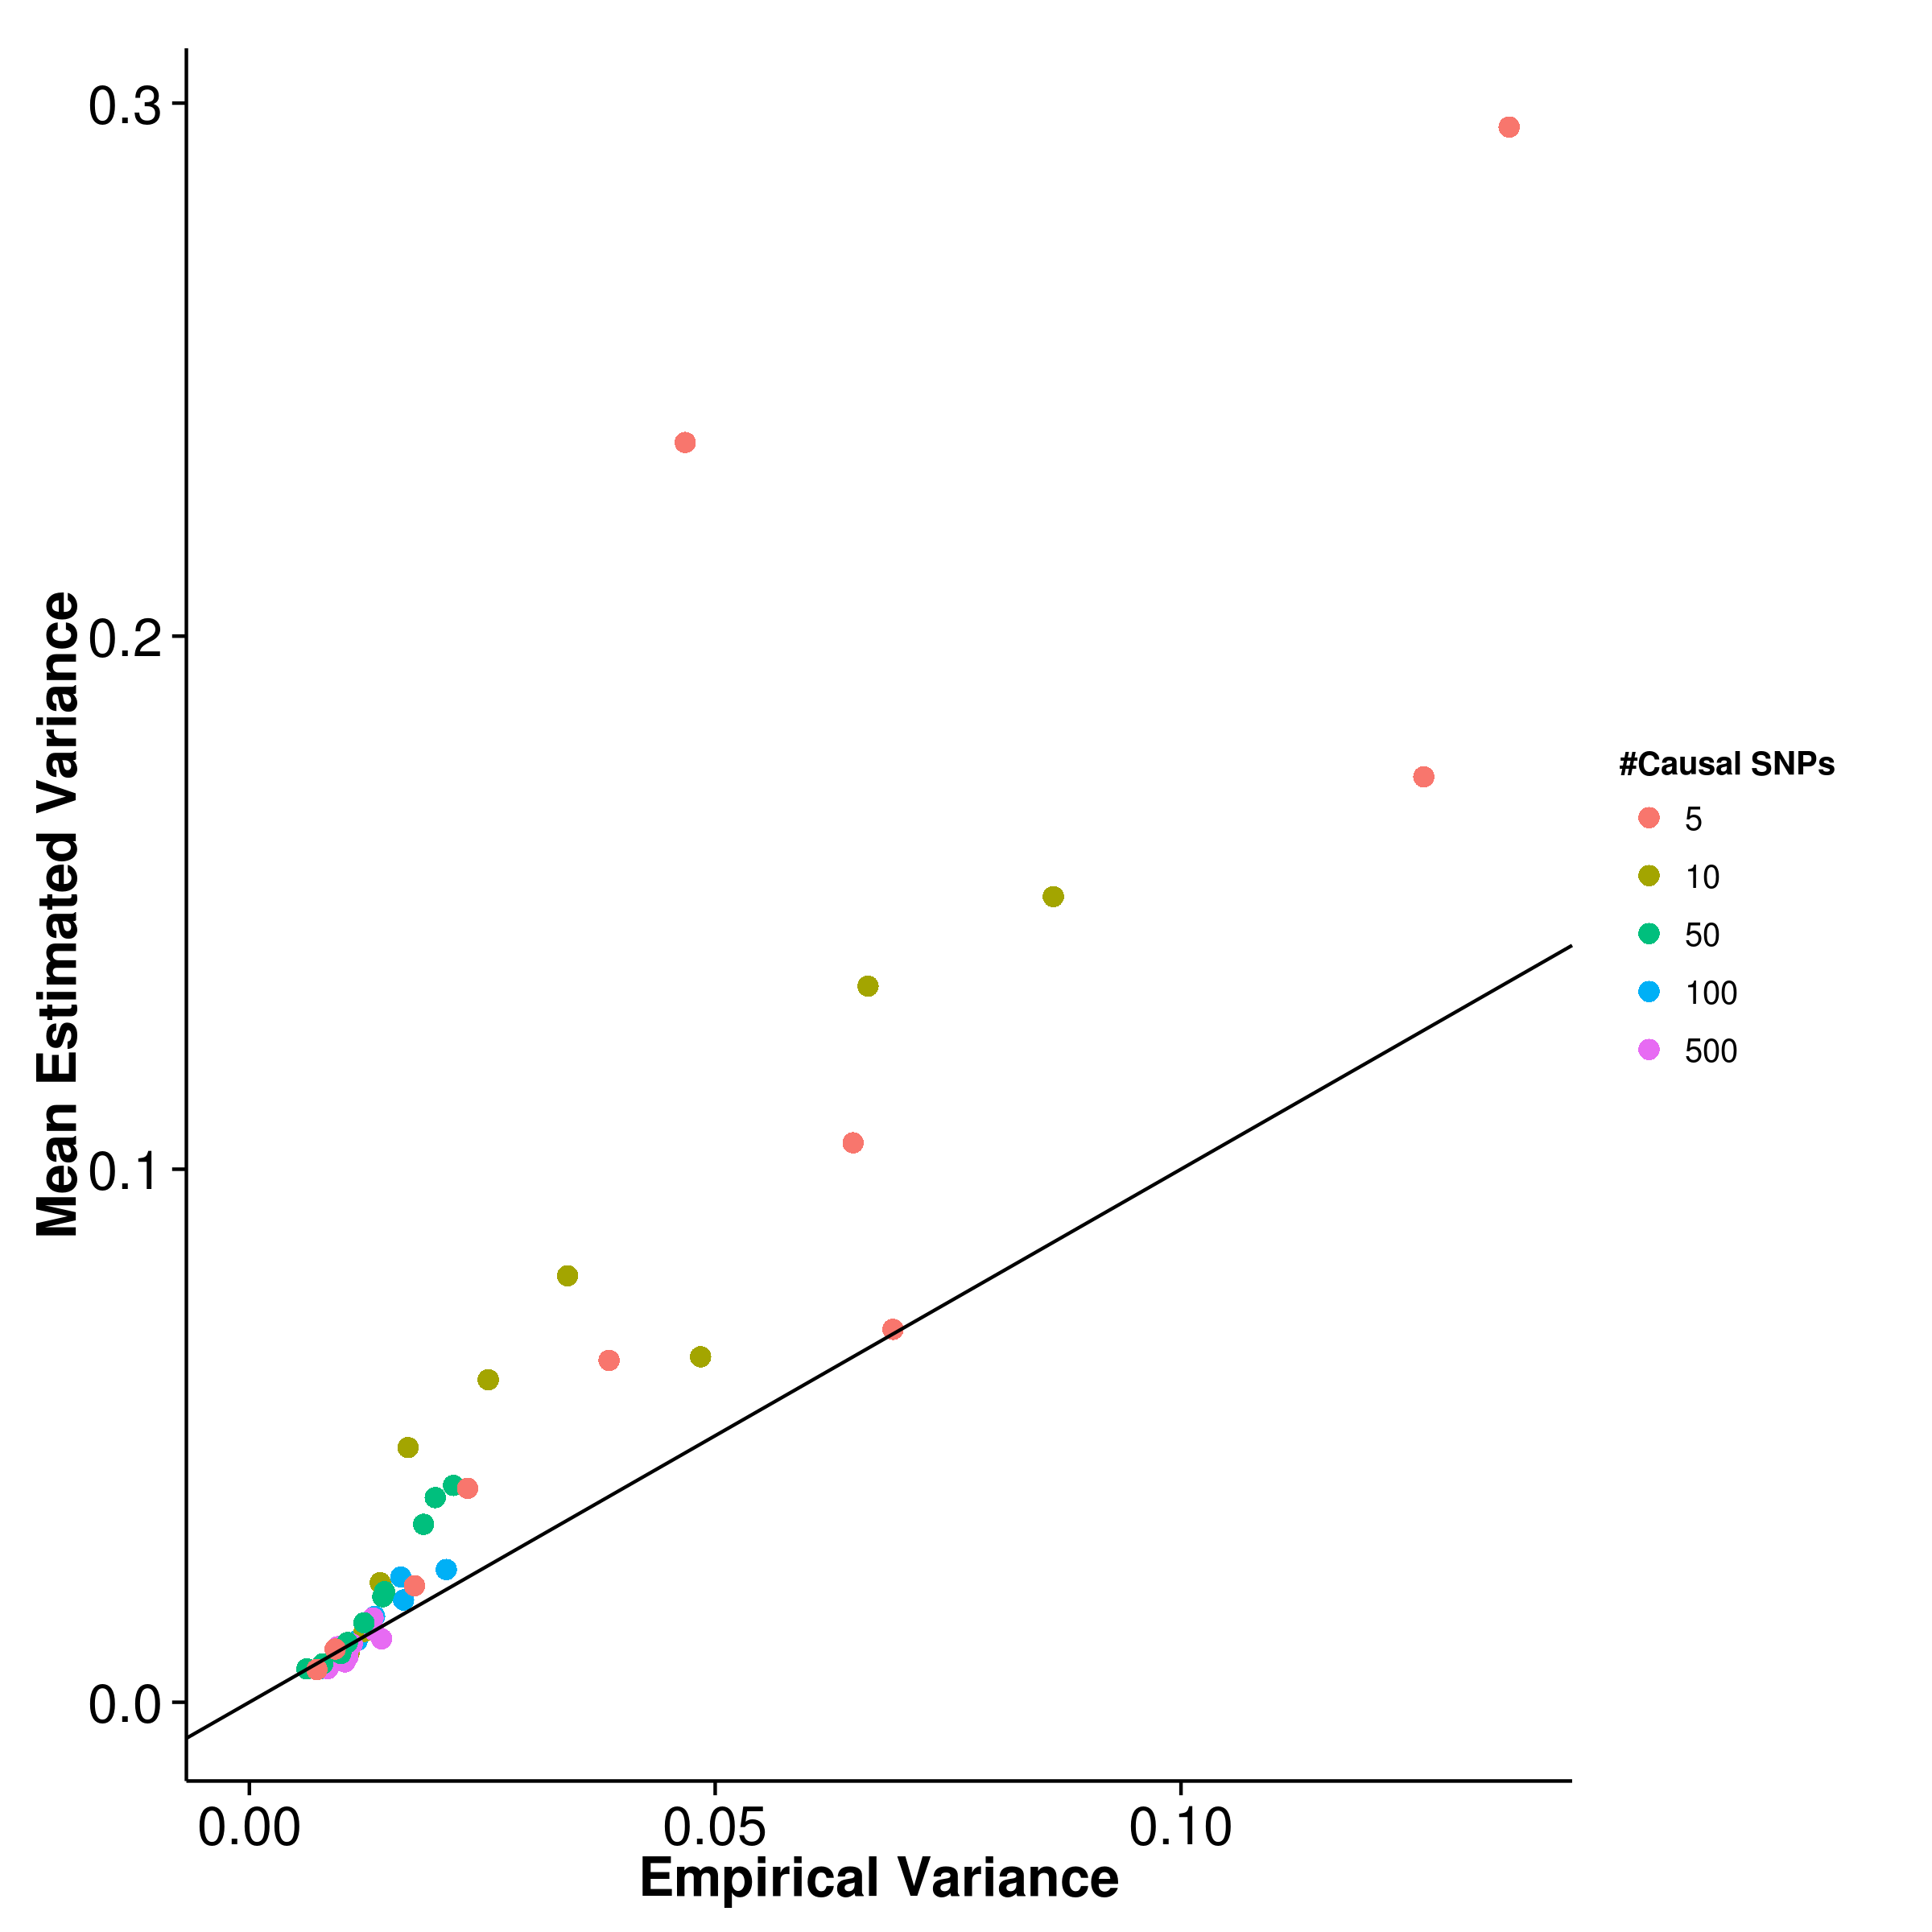
\includegraphics{figure/he_summary/random/ldsc_Qt_Rand_sdCom.png}}
				\label{fig:ldscQtRandVarCom}
			}
			\subfloat[LDSC with intercept estimation]{
				
				\scalebox{.4}{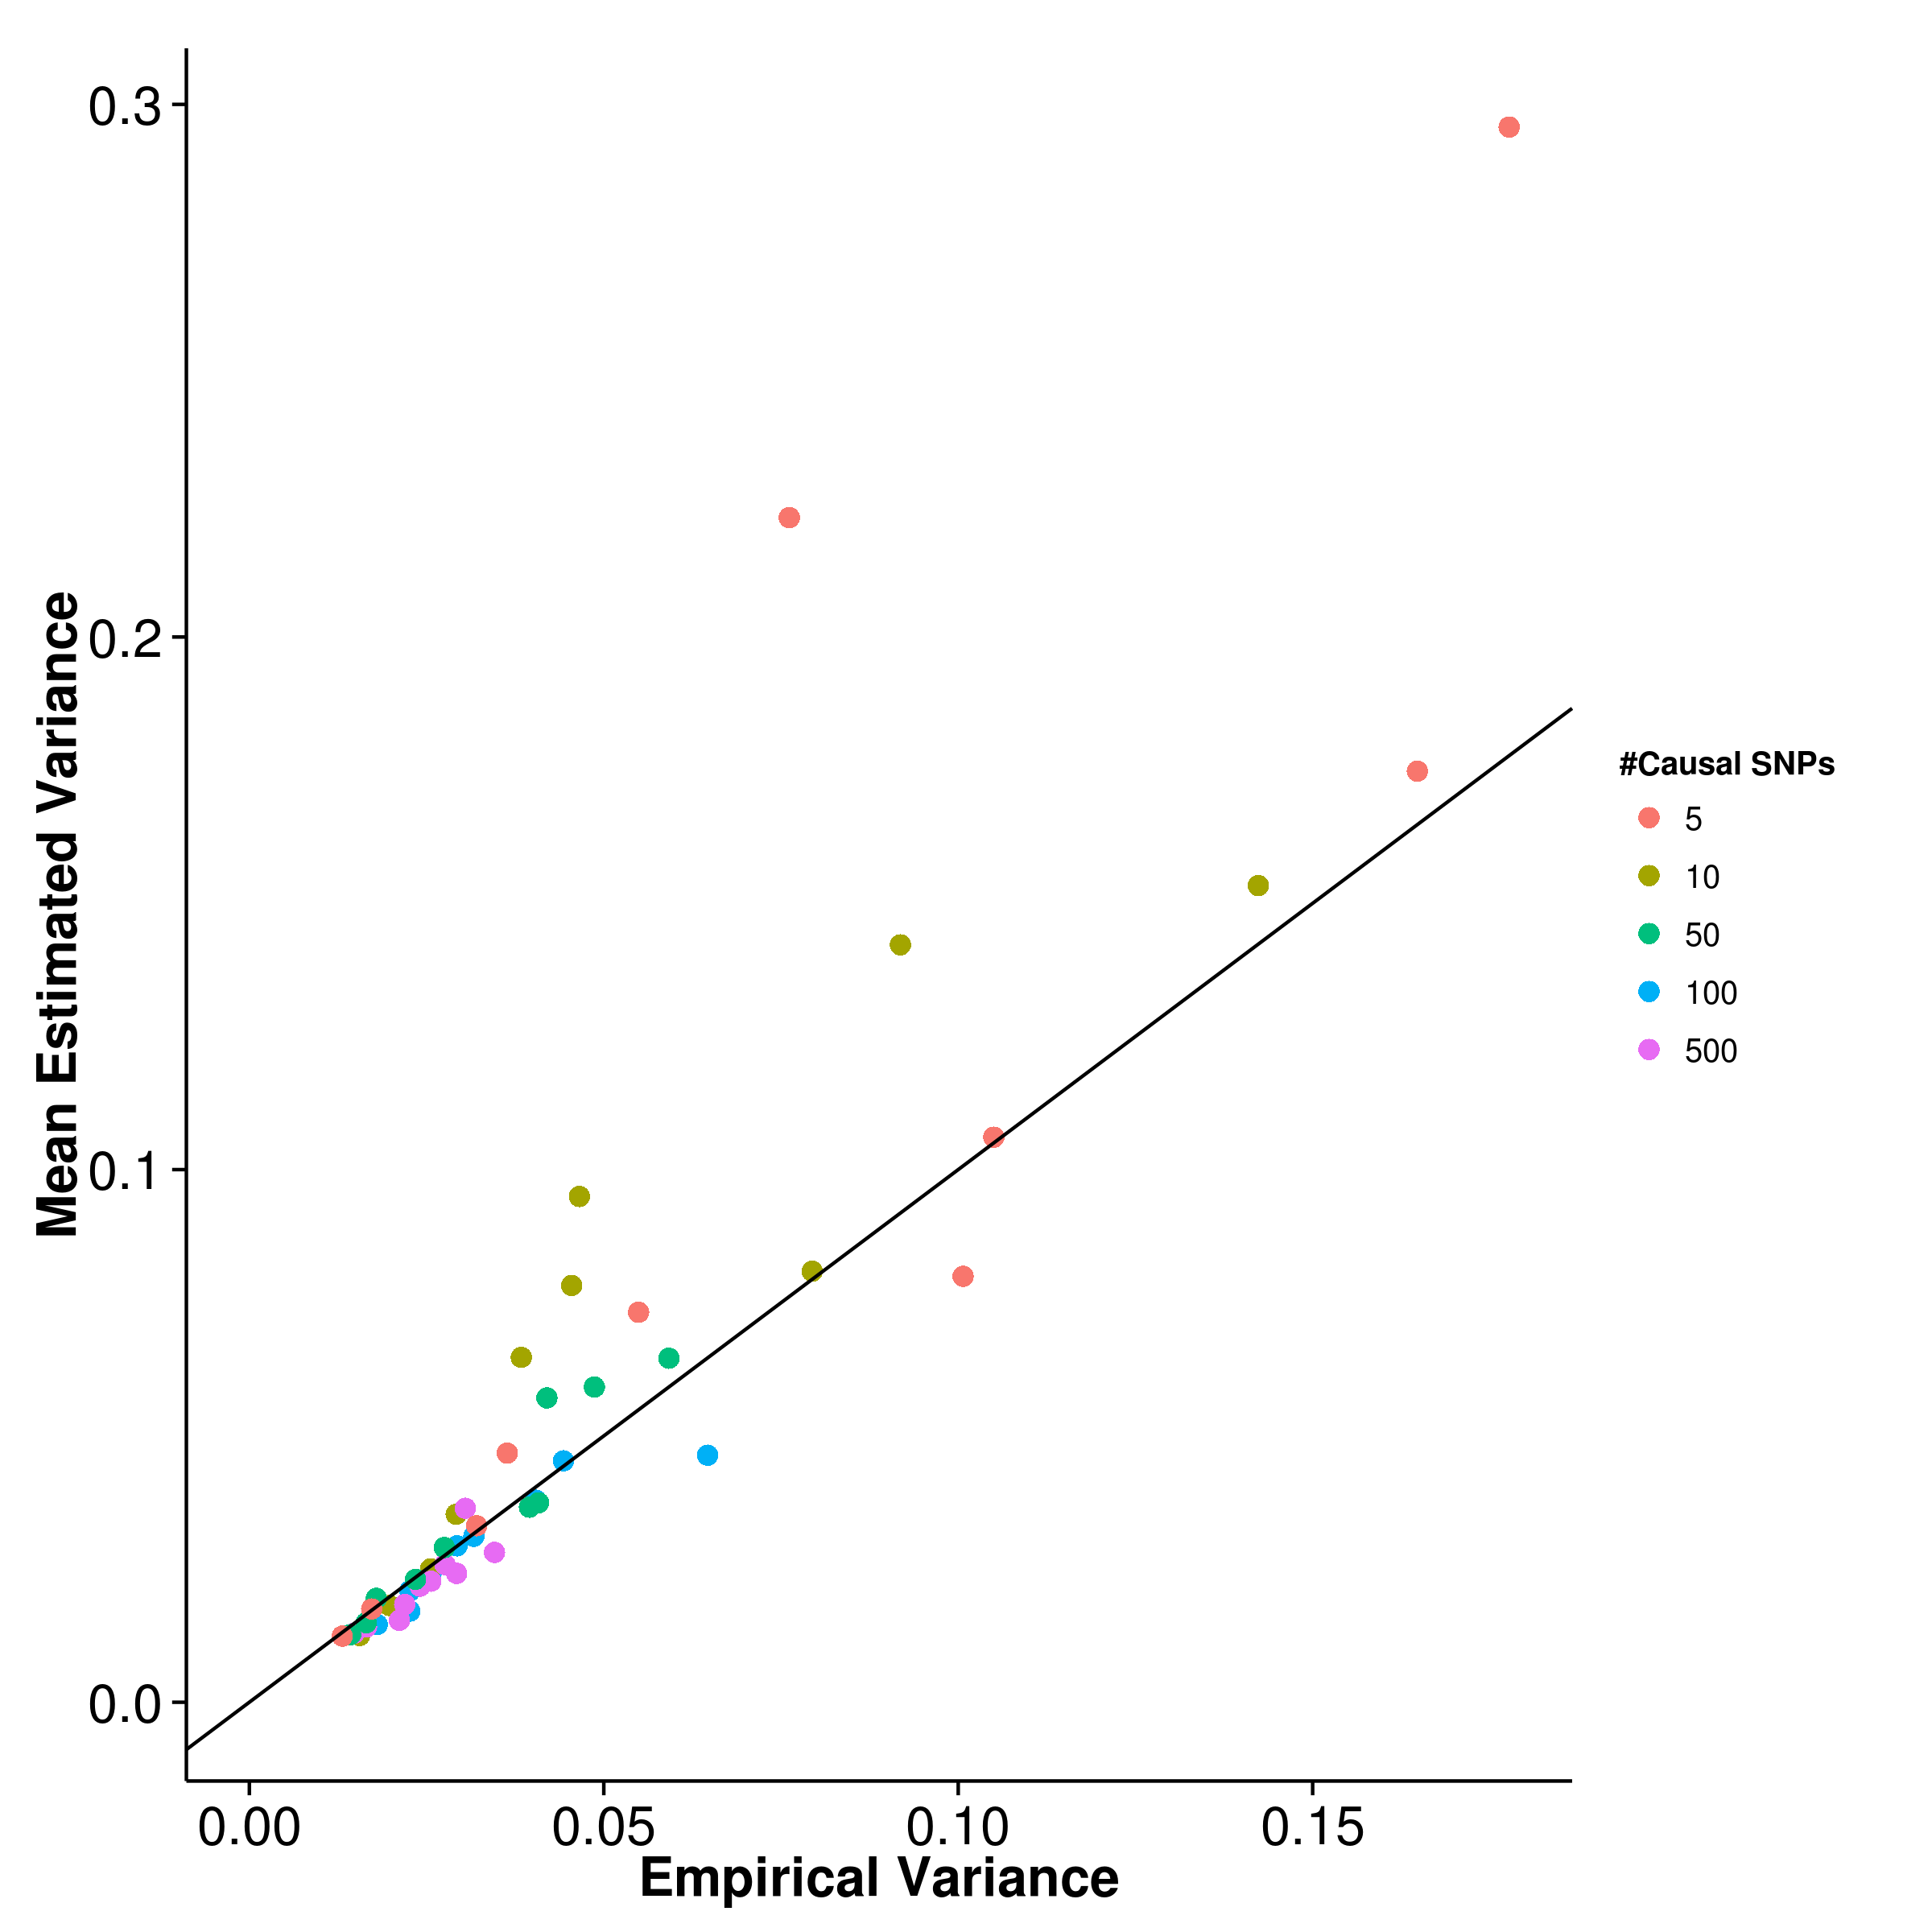
\includegraphics{figure/he_summary/random/ldscIn_Qt_Rand_sdCom.png}}
				\label{fig:ldscInQtRandVarCom}
			}
			\caption[Estimation of Variance in Quantitative Trait Simulation]
			{Estimated variance of results from quantitative trait simulation with random effect size simulation when compared to the empirical variance.
			\gls{gcta} has the best estimate of its empirical variance under the polygenic conditions whereas \gls{shrek} tends to under-estimate its empirical variance.
			On the other hand, \gls{ldsc} to over-estimate the variance especially when the number of causal \glspl{SNP} is small.
				} 
			\label{fig:QtRandVarCom}
		\end{figure}
		Next, we simulate quantitative trait with random effect size assigned to the causal \glspl{SNP}.
		The exponential distribution with $\lambda=1$ was selected because it was suggested that it may serve as a heuristic expectation the genetic architecture of adaptation\citep{Orr1998}.
		There might be many other distribution that can be used, however due to limitation in resources, we will only focus on the exponential distribution with $\lambda=1$.

		Under this simulation condition, it was observed that the mean estimation of heritability from \gls{shrek}(\cref{fig:shrekQtRandMean}) and \gls{gcta}(\cref{fig:gctaQtRandMean}) were similar to what was observed in the equal effect size simulation.
		For \gls{ldsc} with intercept estimation(\cref{fig:ldscInQtRandMean}), less bias was observed with only the 10 causal \glspl{SNP} scenario being under estimated. 
		On the other hand, the performance of \gls{ldsc} with fixed intercept remain more or less the same, with a larger degree of fluctuation when small number of causal \glspl{SNP}(5 or 10) was simulated. 
		The fluctuation in estimate can also be observed in the empirical variance of \gls{ldsc}(\cref{fig:ldscQtRandVar,fig:ldscInQtRandVar}).
		Despite the relative stable performance of \gls{gcta}, the empirical variance of \gls{gcta} also fluctuate when the number of causal \glspl{SNP} was small. 
		Such pattern was not observed in \gls{shrek} suggesting that it might be robust against the change in number of causal \glspl{SNP}.
		
		When inspecting the relationship between the estimated and empirical variance, it was observed all programmes have a less accurate estimation of its variance when there is only 5 causal \glspl{SNP}. 
		The difference was most obvious for \gls{gcta} where the under-estimation of variance under the oligo-genic scenario(5 or 10 causal \glspl{SNP}) was more severe when a random effect size was assigned to the causal \glspl{SNP}(\cref{fig:gctaQtRandVarCom}).    
		On the other hand, the degree of bias in estimating the variance remain more or less unchanged for \gls{shrek}(\cref{fig:shrekQtRandVarCom}) and \gls{ldsc} with intercept estimation(\cref{fig:ldscInQtRandVarCom}), with roughly 0.9 and 1.25 times difference from the empirical variance respectively.
		However, for \gls{ldsc} with fixed intercept(\cref{fig:ldscQtRandVarCom}), the fold difference increased slightly, changed from 1.5 fold difference to 1.65 fold difference.
		
		Overall, simulating the effect size using the exponential distribution only slightly increases the \gls{mse} of the programmes when the number of causal \glspl{SNP} is small and decreases the \gls{mse} when the number of causal \glspl{SNP} is larger. 
		Taking into considering of both the bias and standard error, \gls{shrek} has the better performance over \gls{ldsc} except when the trait is extremely polygenic(e.g. $\ge500$ causal \glspl{SNP}).
		\begin{table}
			\centering
			\begin{tabular}{rrrrr}
				\toprule
				Number of Causal SNPs&	SHREK&	LDSC&	LDSC-In&	GCTA \\
				\midrule
				5	&	0.177	&	0.565	&	0.584	&	0.230\\
				10	&	0.159	&	0.251	&	0.470	&	0.151\\
				50	&	0.153	&	0.179	&	0.378	&	0.0796\\
				100	&	0.157	&	0.166	&	0.305	&	0.0794\\
				250	&	0.152	&	0.144	&	0.266	&	0.0674\\
				500	&	0.143	&	0.134	&	0.247	&	0.0646\\
				\bottomrule
			\end{tabular}
			\caption[Mean Squared Error of Quantitative Trait Simulation with Random Effect Size]{
				\gls{mse} of quantitative trait simulation with random effect size.
				Again, \gls{gcta} has the lowest \gls{mse} except when there is only 5 causal \glspl{SNP} and the performance of \gls{shrek} and \gls{ldsc} with fix intercept converges as number of causal \glspl{SNP} increases. 
				\gls{ldsc} with fix intercept even surpassed \gls{shrek}'s performance when the number of causal \glspl{SNP} was as high as 500.}
			\label{tab:mseQtRandom}
		\end{table}
		% Extreme with 100 causal
		\subsection{Quantitative Trait Simulation with Extreme Effect Size}
		
		\begin{figure}
			\centering
			\subfloat[SHREK]{
				\scalebox{.4}{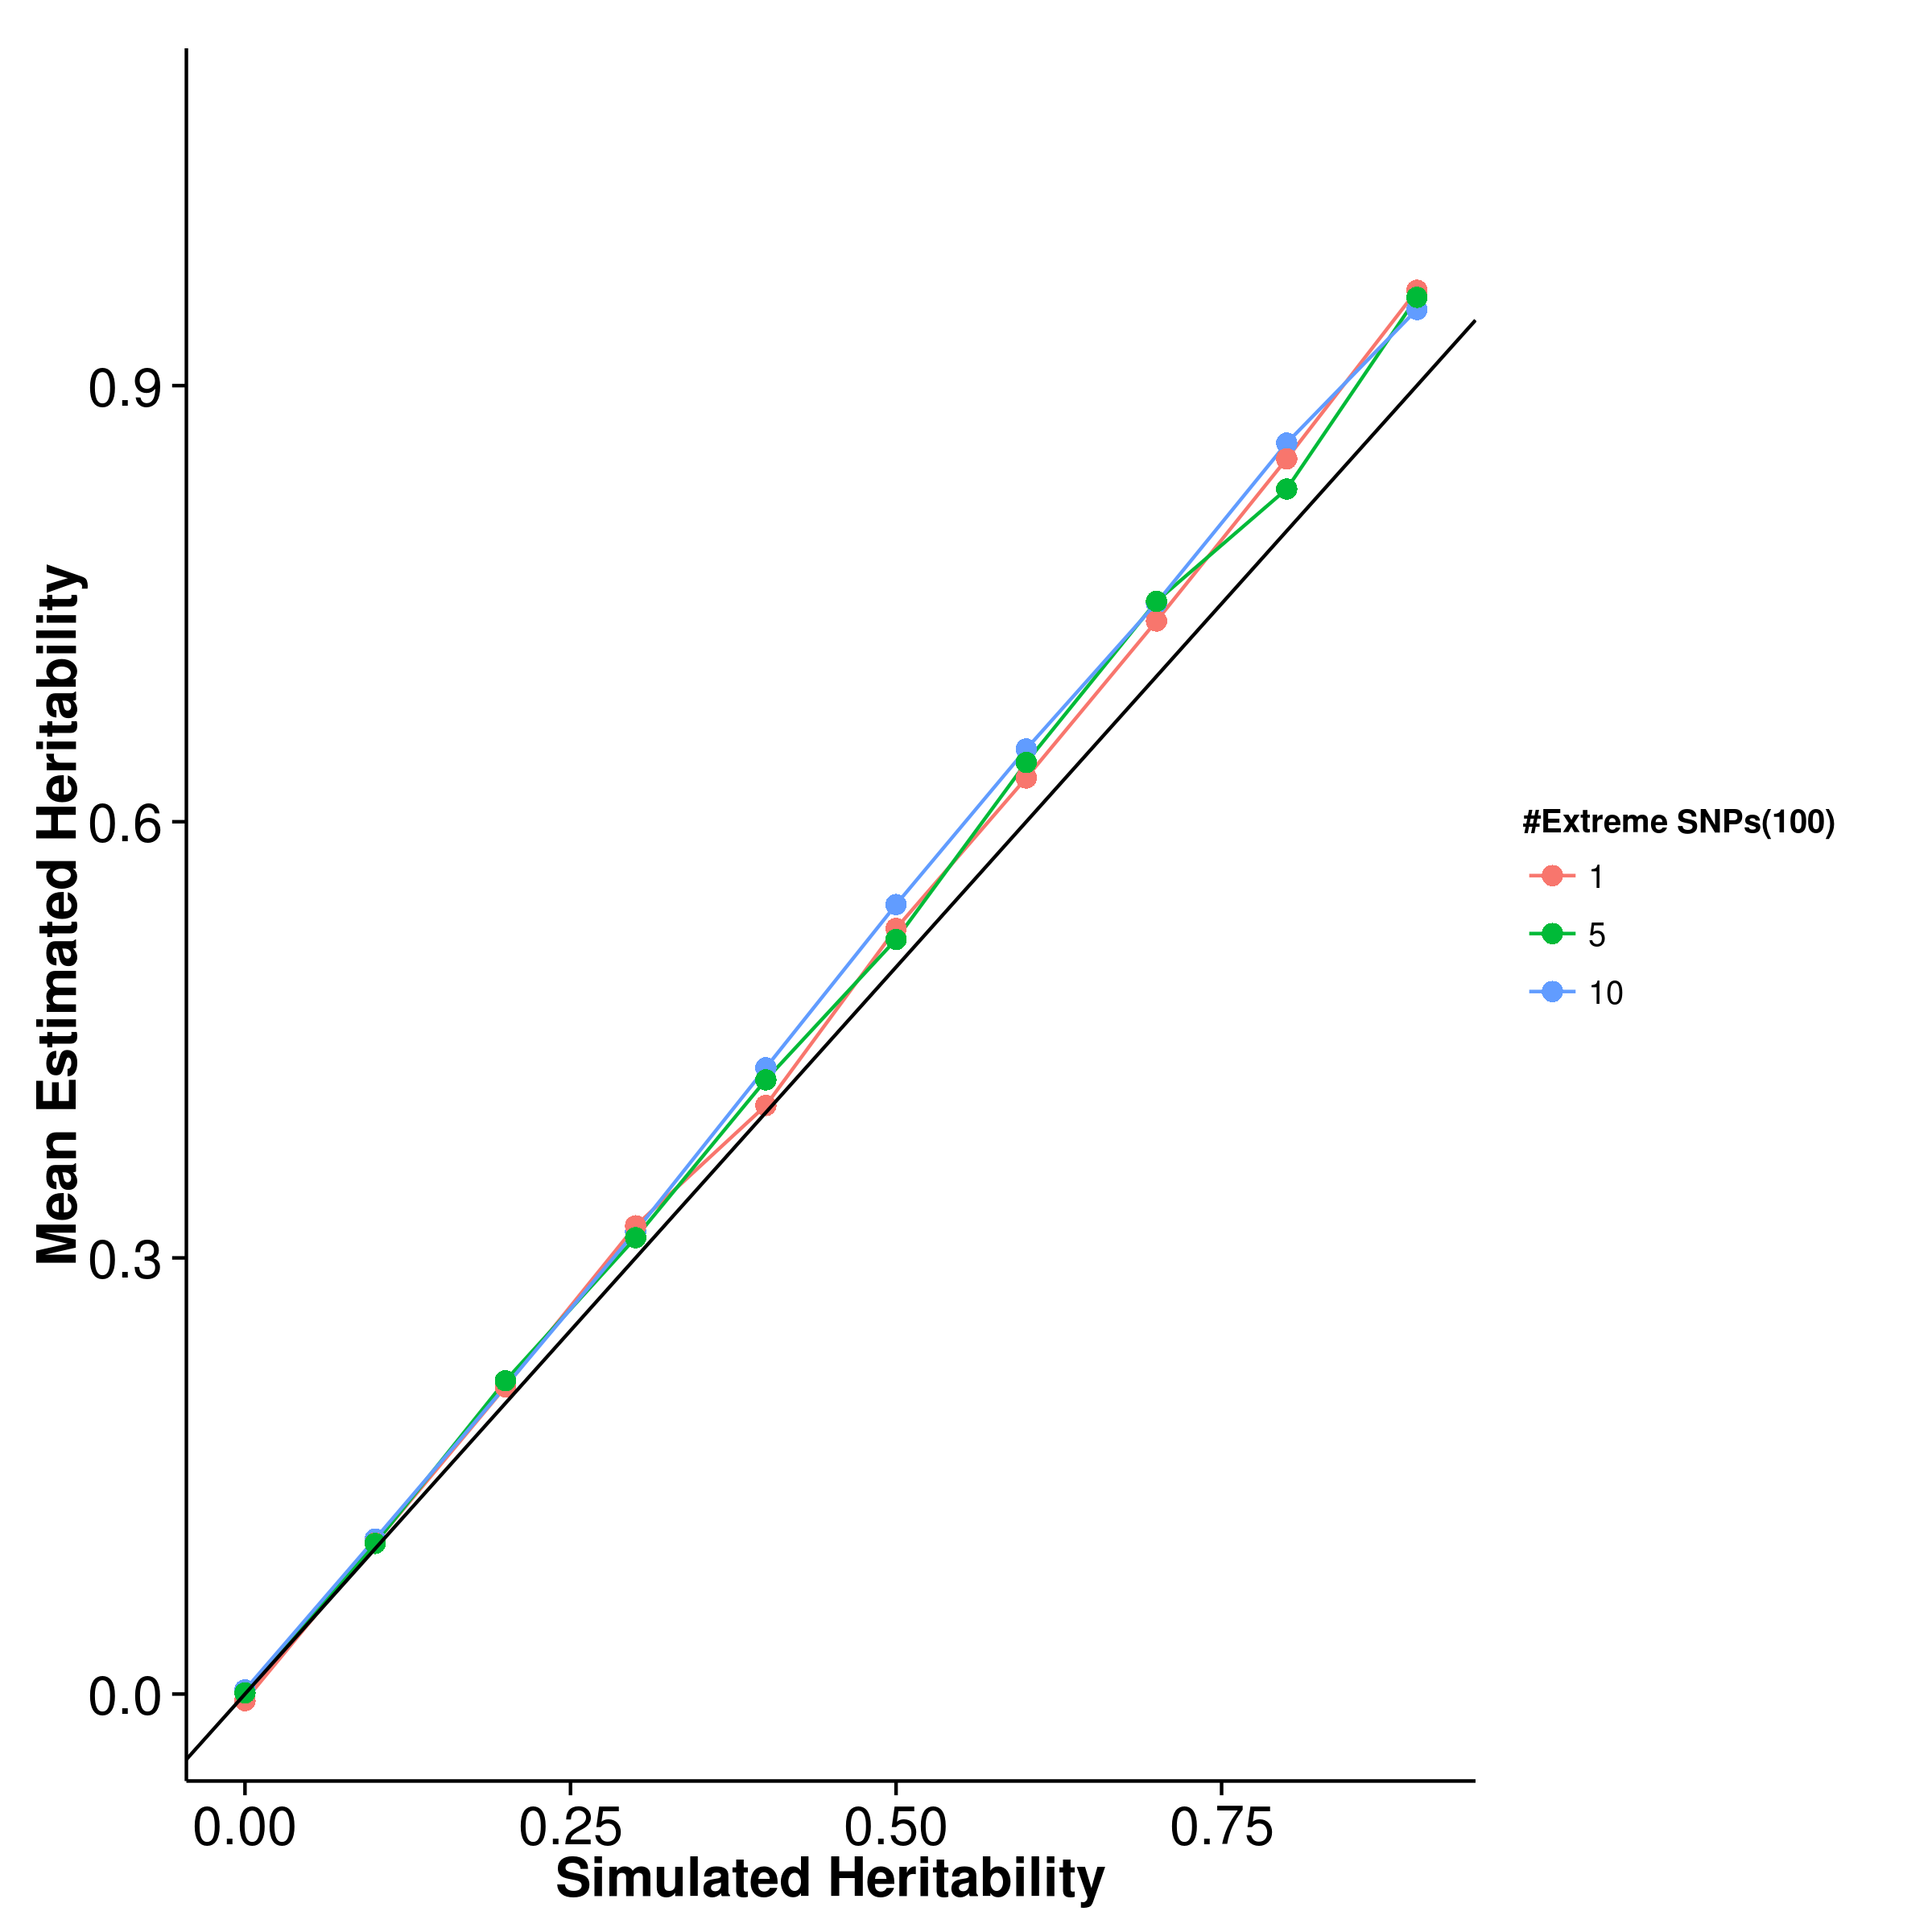
\includegraphics{figure/he_summary/extreme_100c/shrek_QtE_Rand_mean.png}}
				\label{fig:shrekQtEx100cMean}
			}
			\subfloat[GCTA]{
				\scalebox{.4}{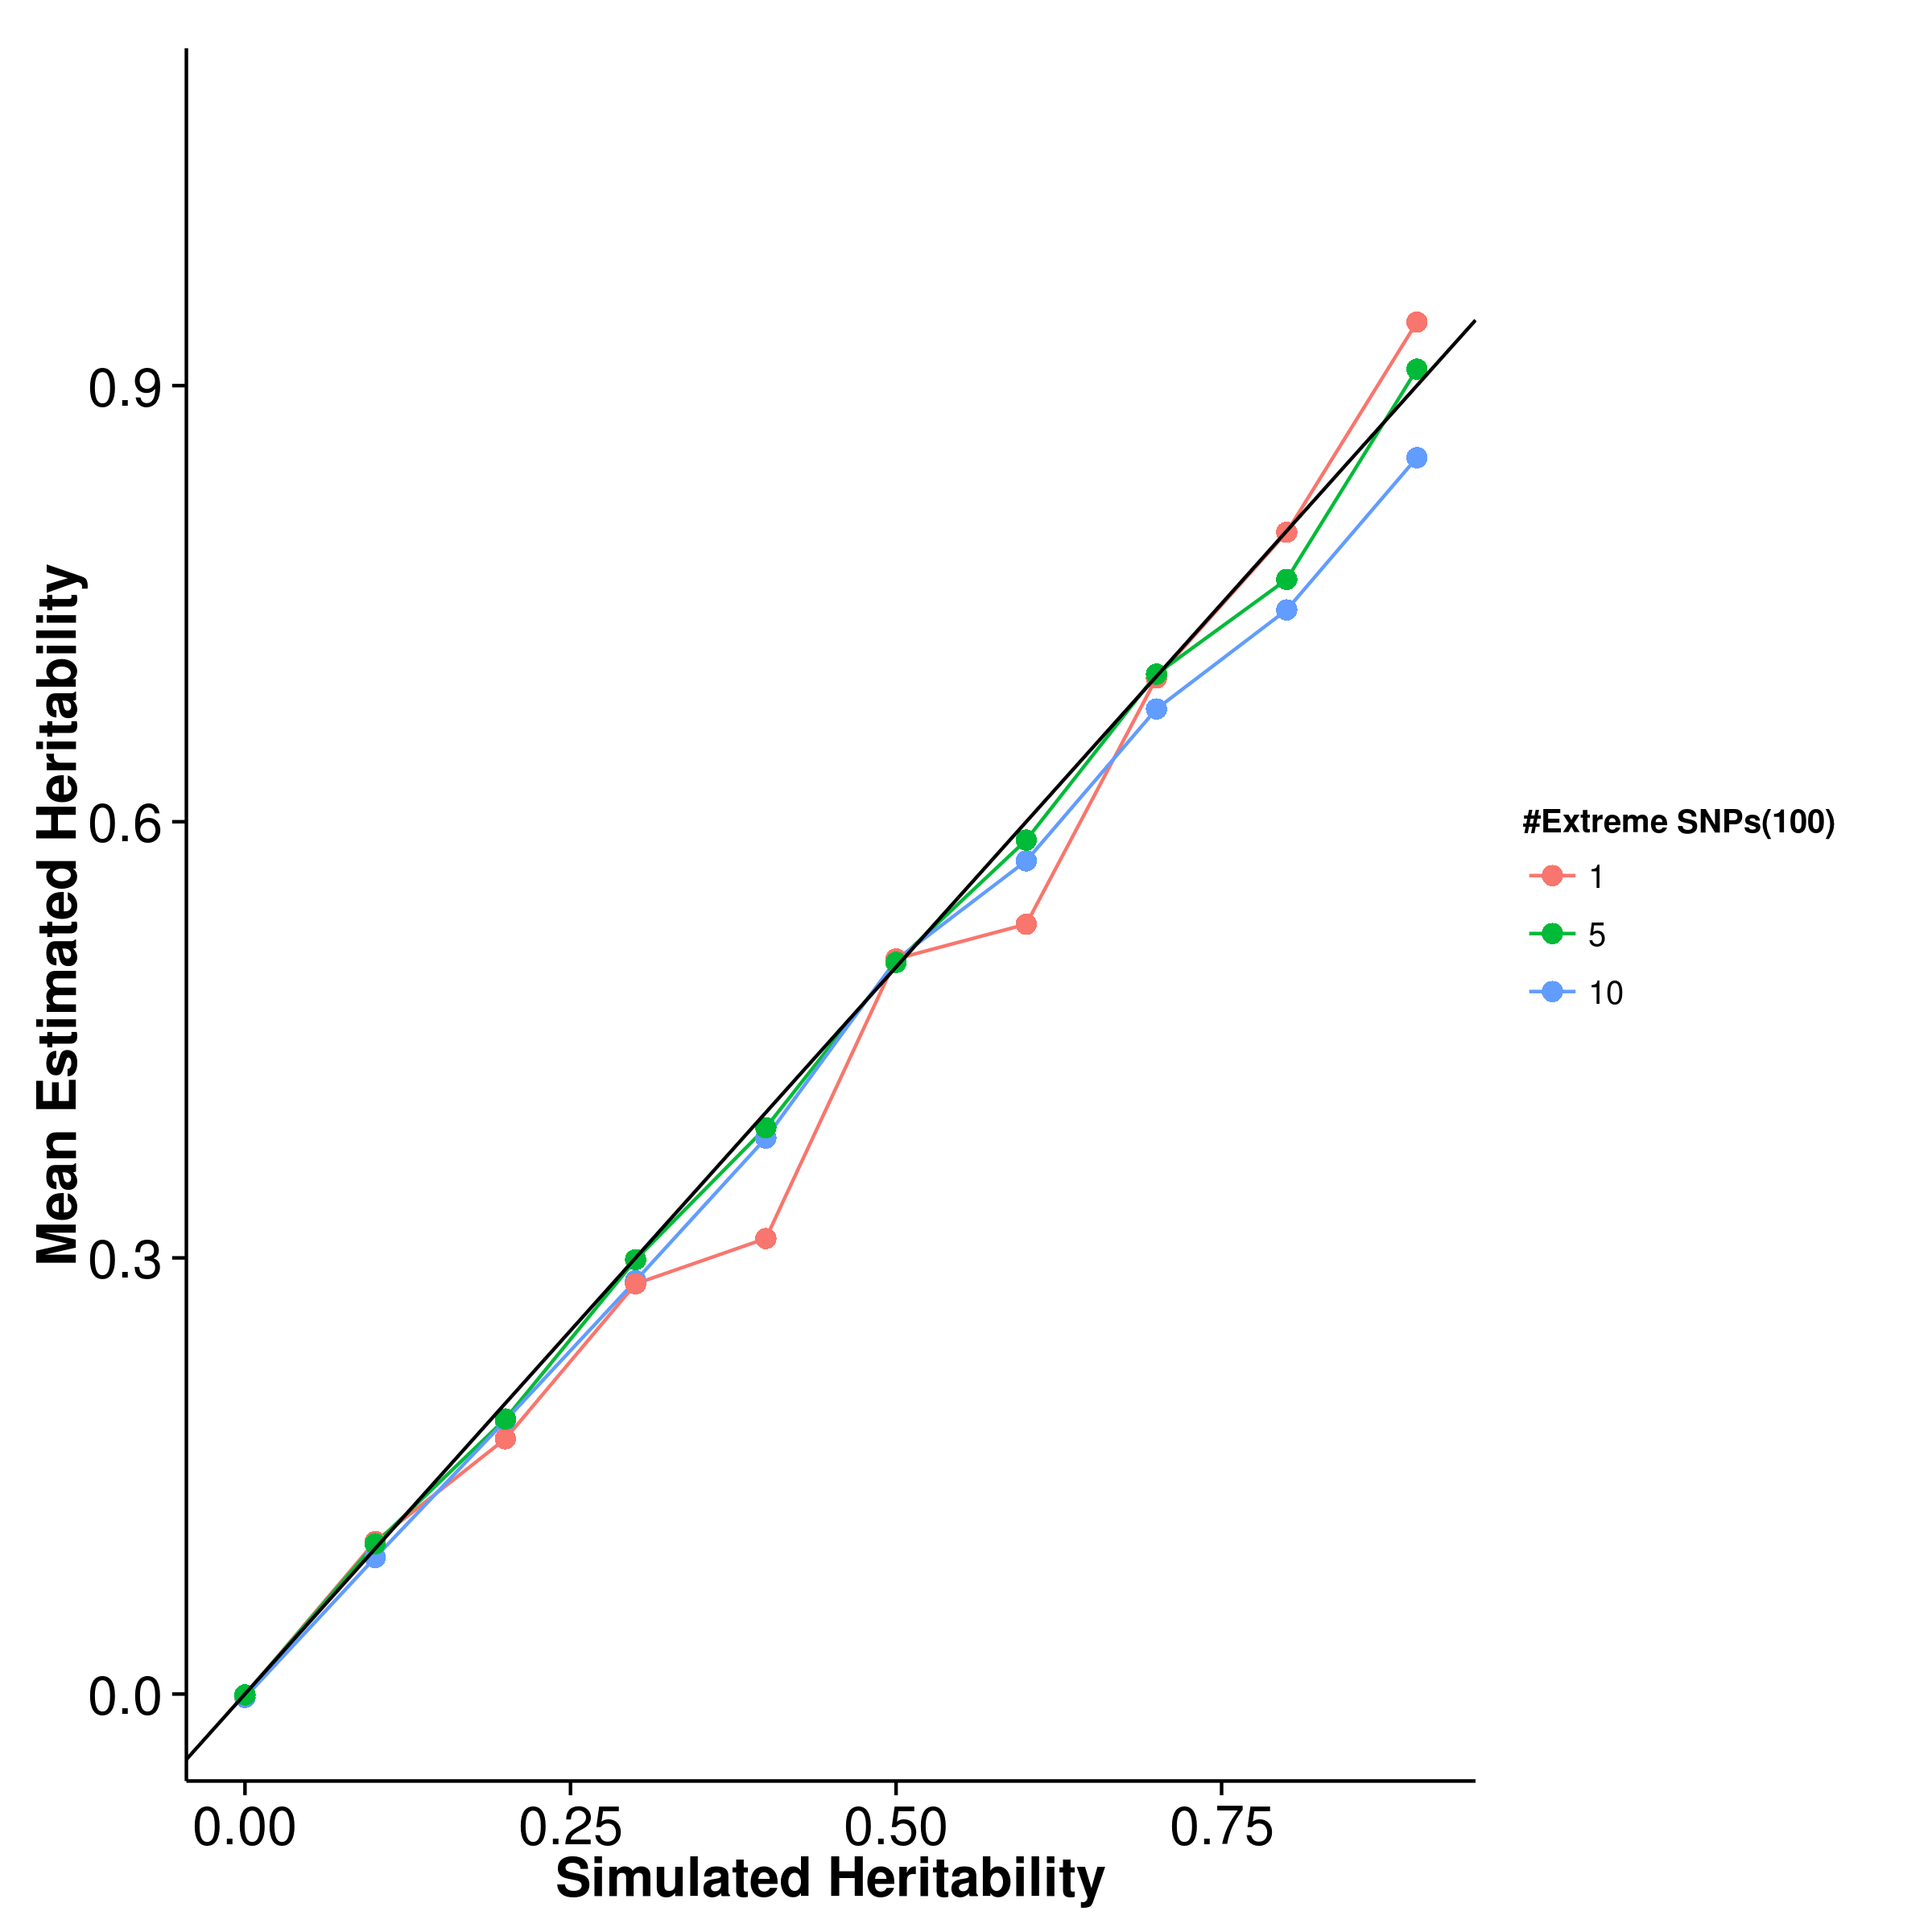
\includegraphics{figure/he_summary/extreme_100c/gcta_QtE_Rand_mean.png}}
				\label{fig:gctaQtEx100cMean}
			}\\
			\subfloat[LDSC with fix intercept]{
				\scalebox{.4}{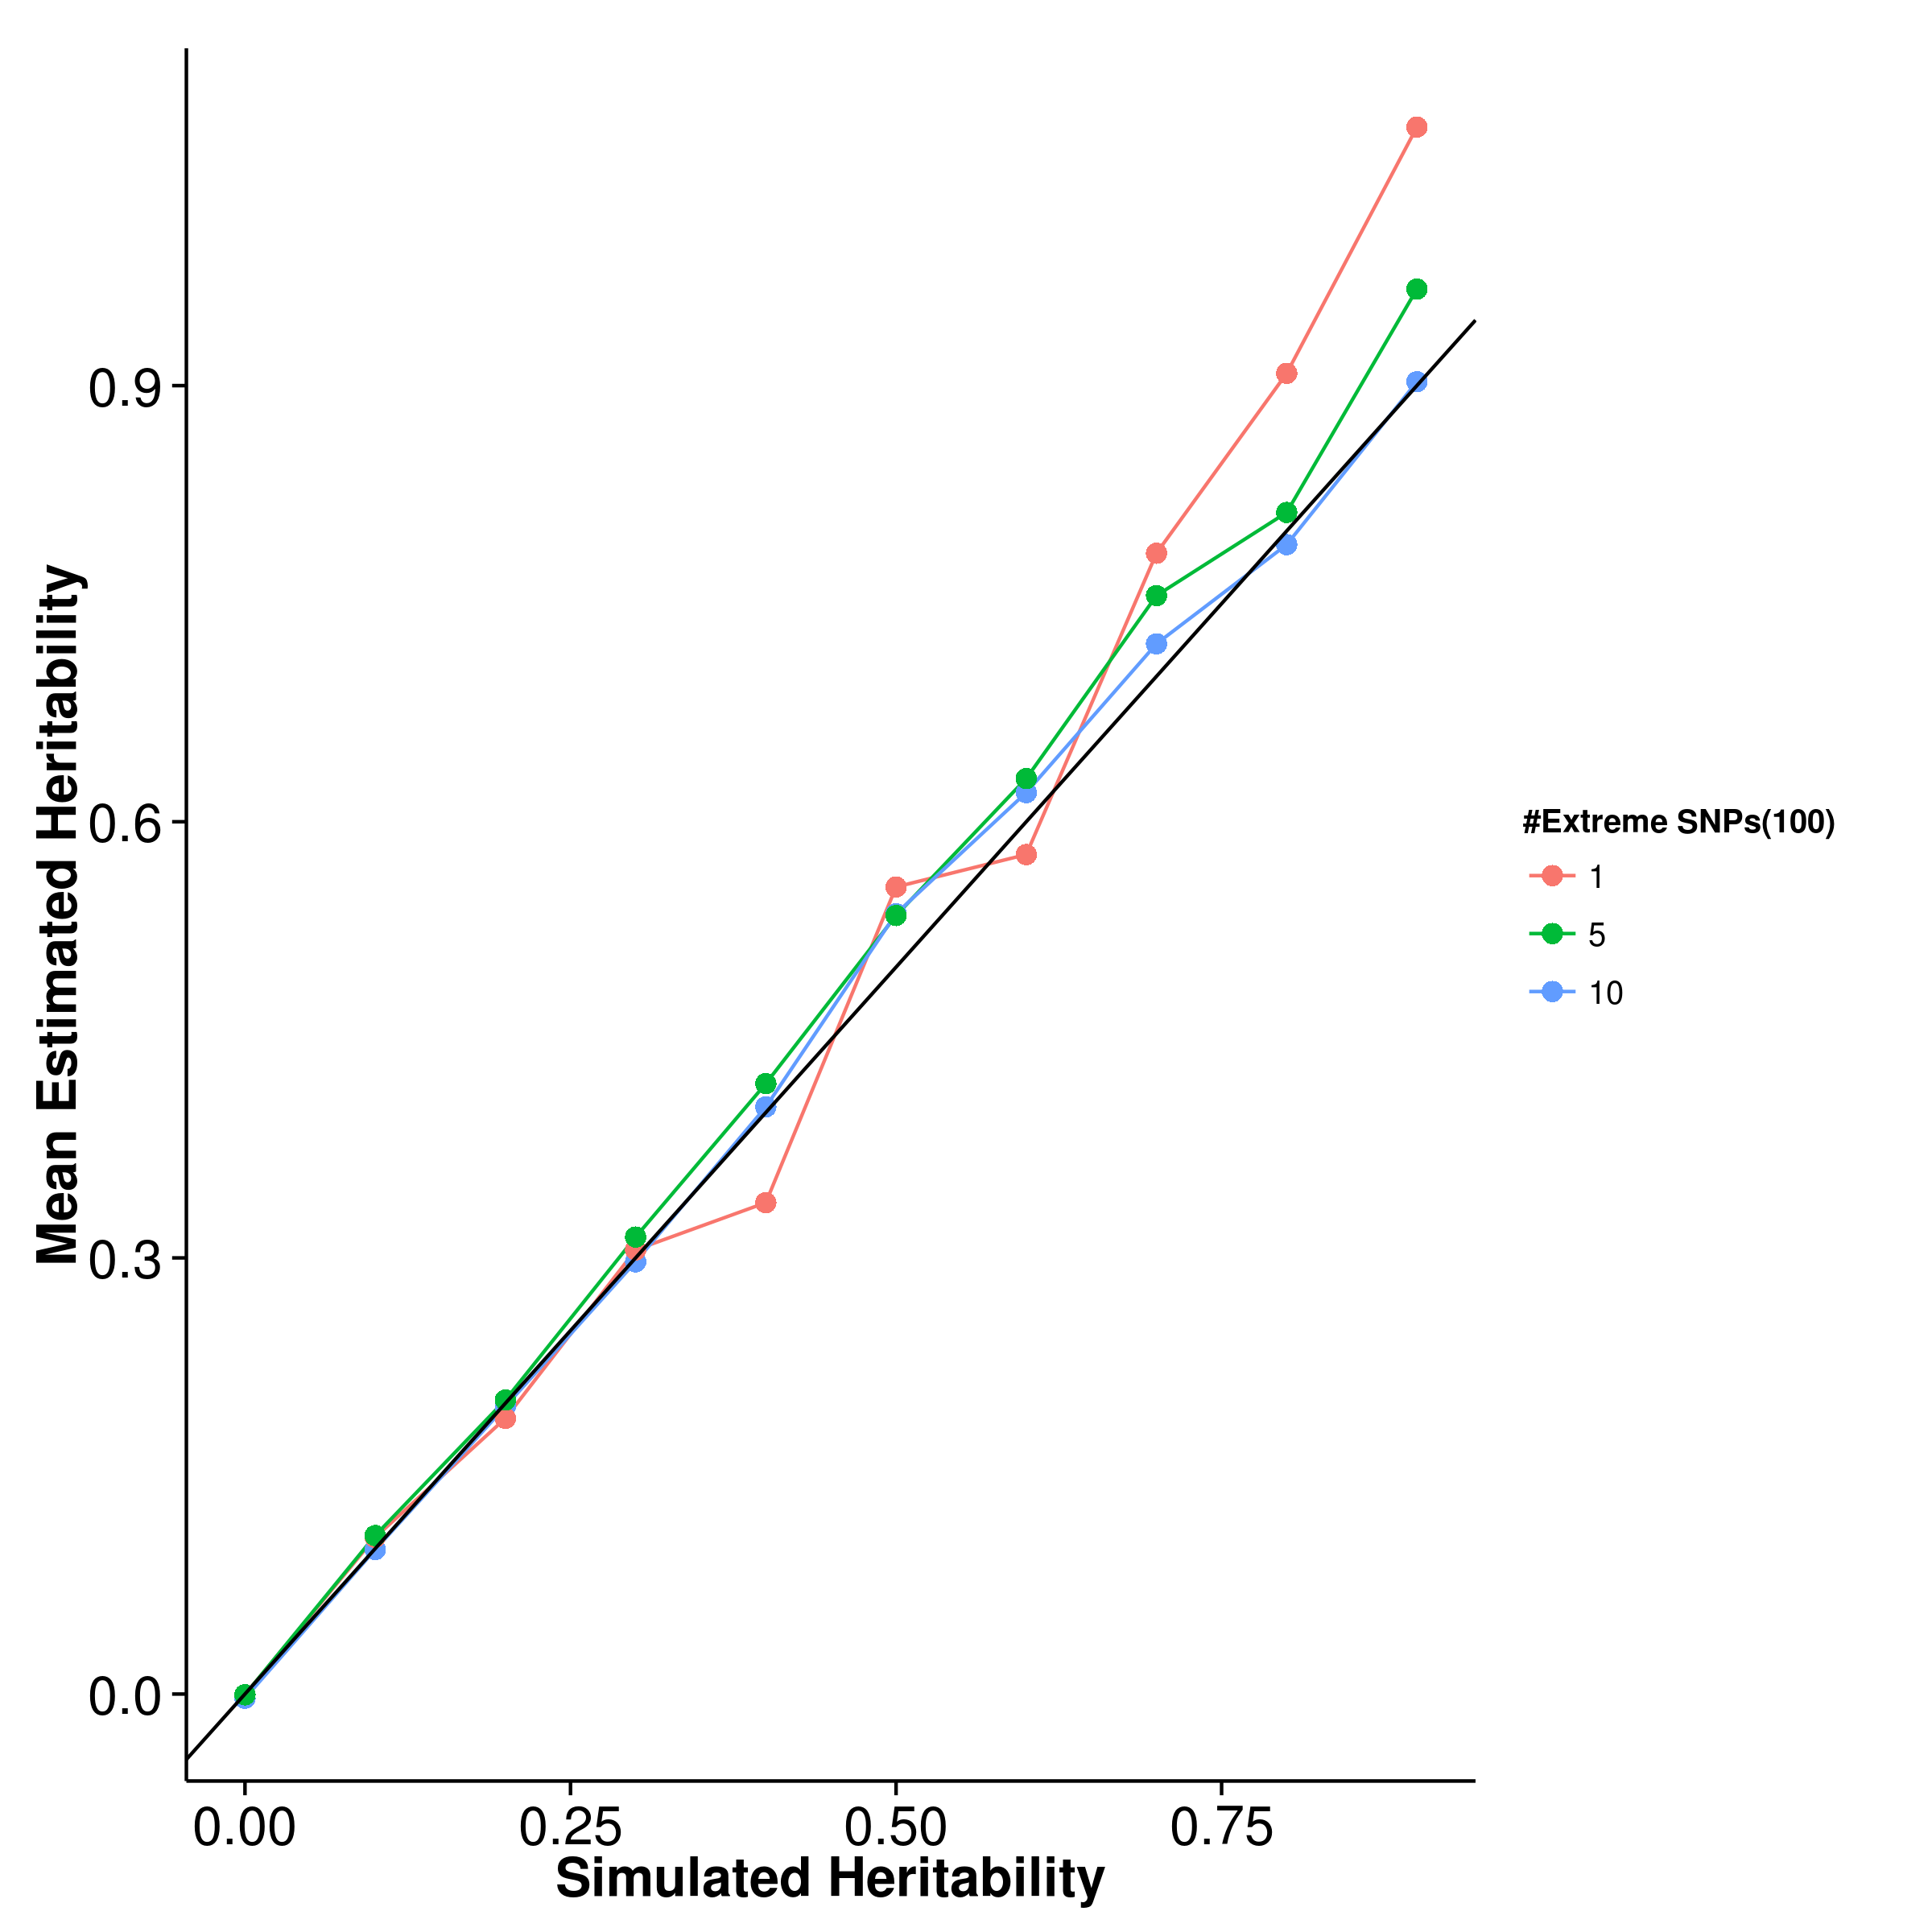
\includegraphics{figure/he_summary/extreme_100c/ldsc_QtE_Rand_mean.png}}
				\label{fig:ldscQtEx100cMean}
			}
			\subfloat[LDSC with intercept estimation]{
				
				\scalebox{.4}{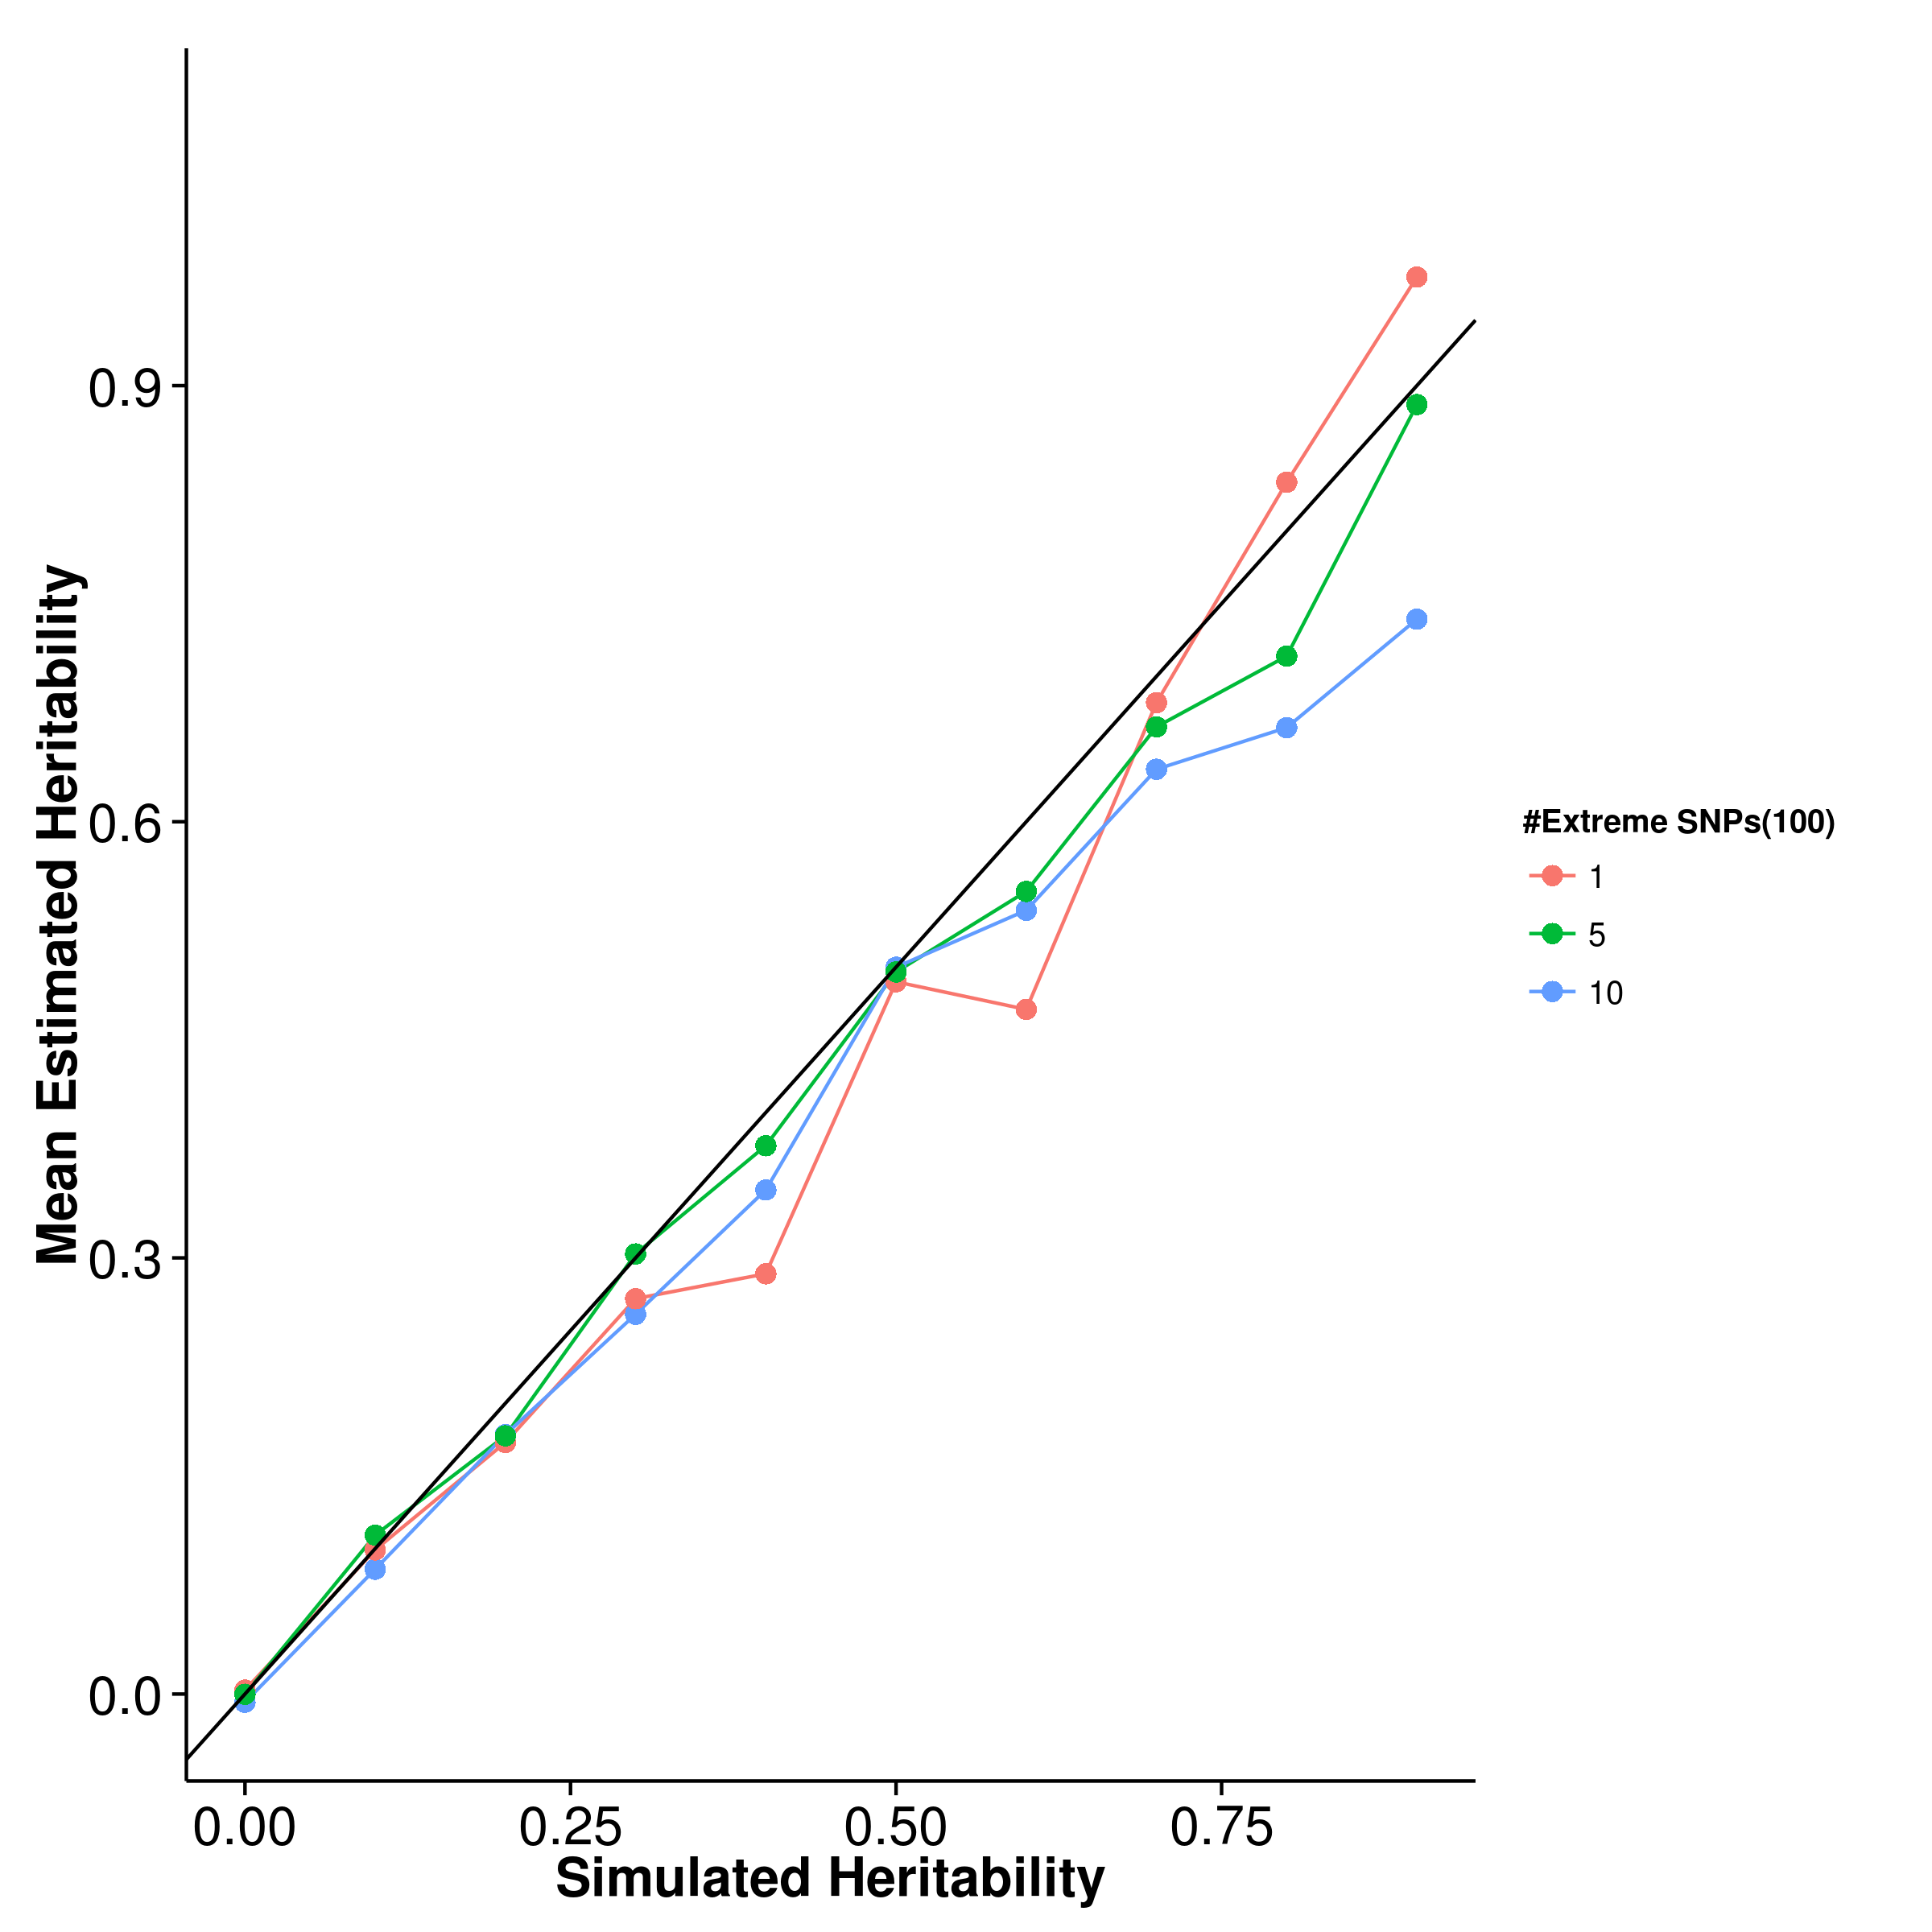
\includegraphics{figure/he_summary/extreme_100c/ldscIn_QtE_Rand_mean.png}}
				\label{fig:ldscInQtEx100cMean}
			}
			\caption[Mean of Extreme Effect Size Simulation Result]
			{Mean of results from quantitative trait simulation with extreme effect size simulation.
				It was observed that the mean estimation of heritability of \gls{shrek} is not affected by the number of \gls{SNP}(s) with large effect but with slight upward bias.
				On the other hand, the mean estimation of \gls{ldsc} and \gls{gcta} seems to fluctuate with respect to the simulated heritability.
				} 
			\label{fig:QtEx100cMean}
		\end{figure}
		
		\begin{figure}
			\centering
			\subfloat[SHREK]{
				\scalebox{.4}{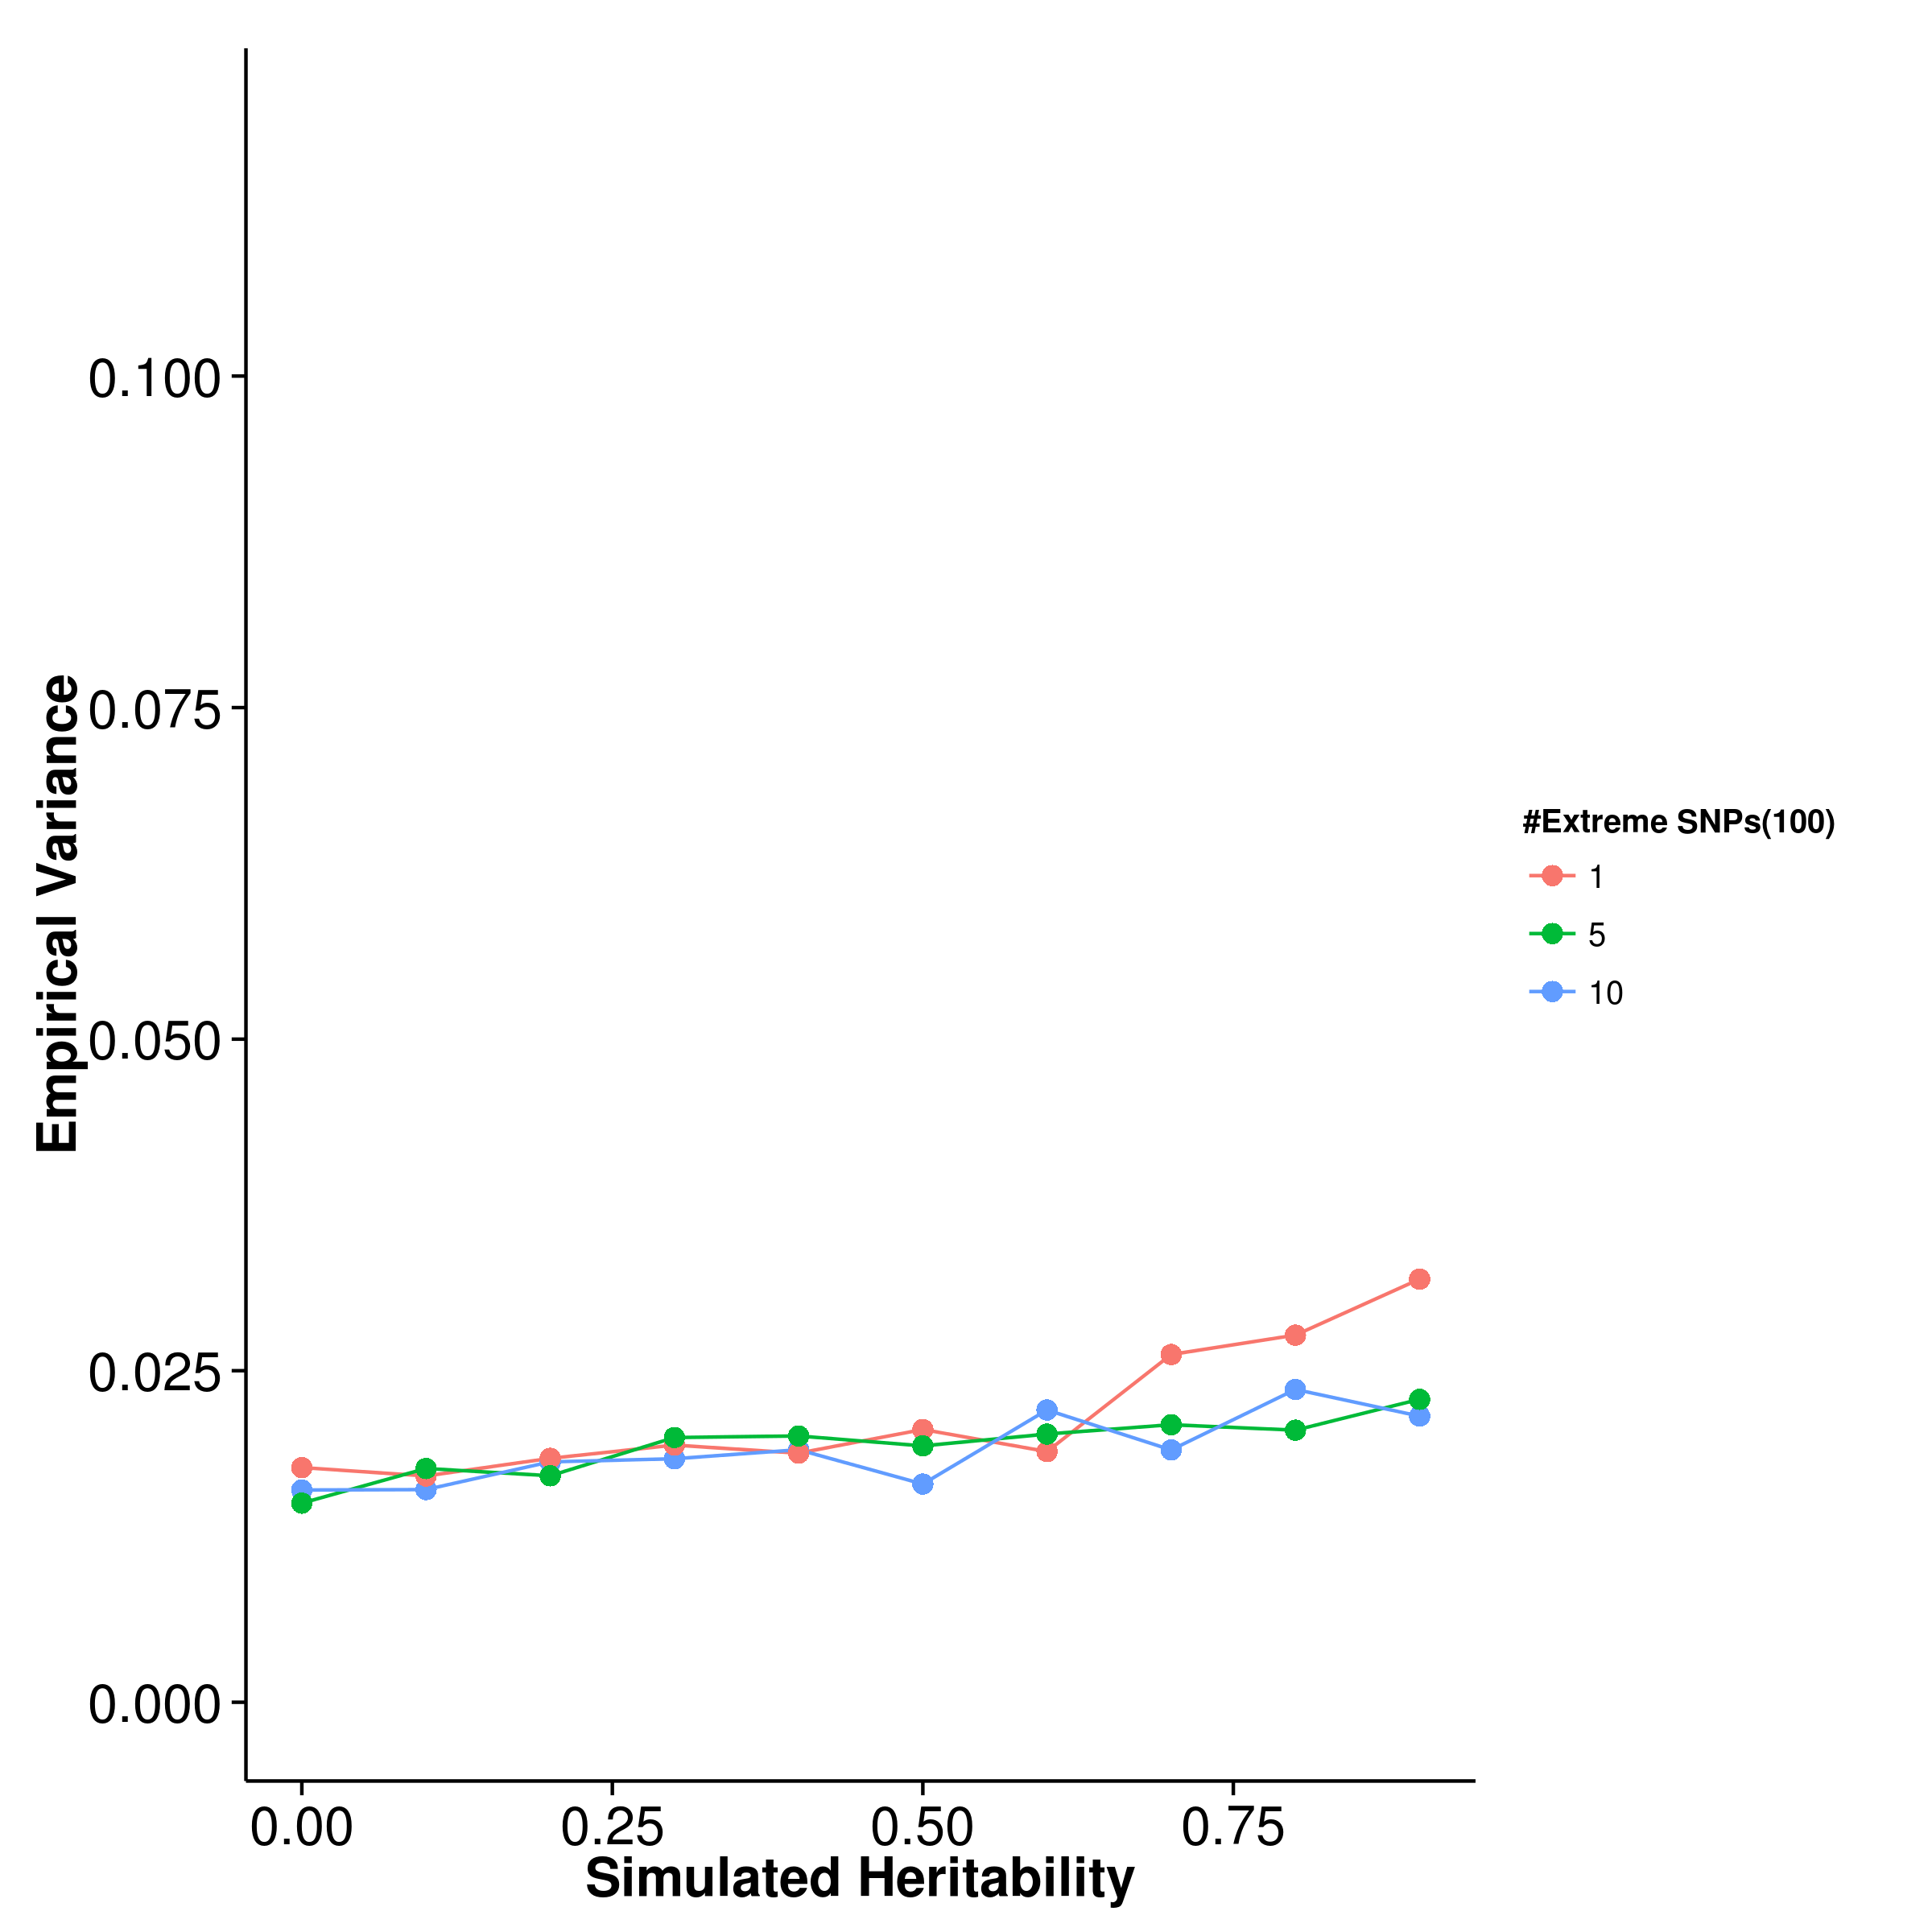
\includegraphics{figure/he_summary/extreme_100c/shrek_QtE_Rand_sd.png}}
				\label{fig:shrekQtEx100cVar}
			}
			\subfloat[GCTA]{
				\scalebox{.4}{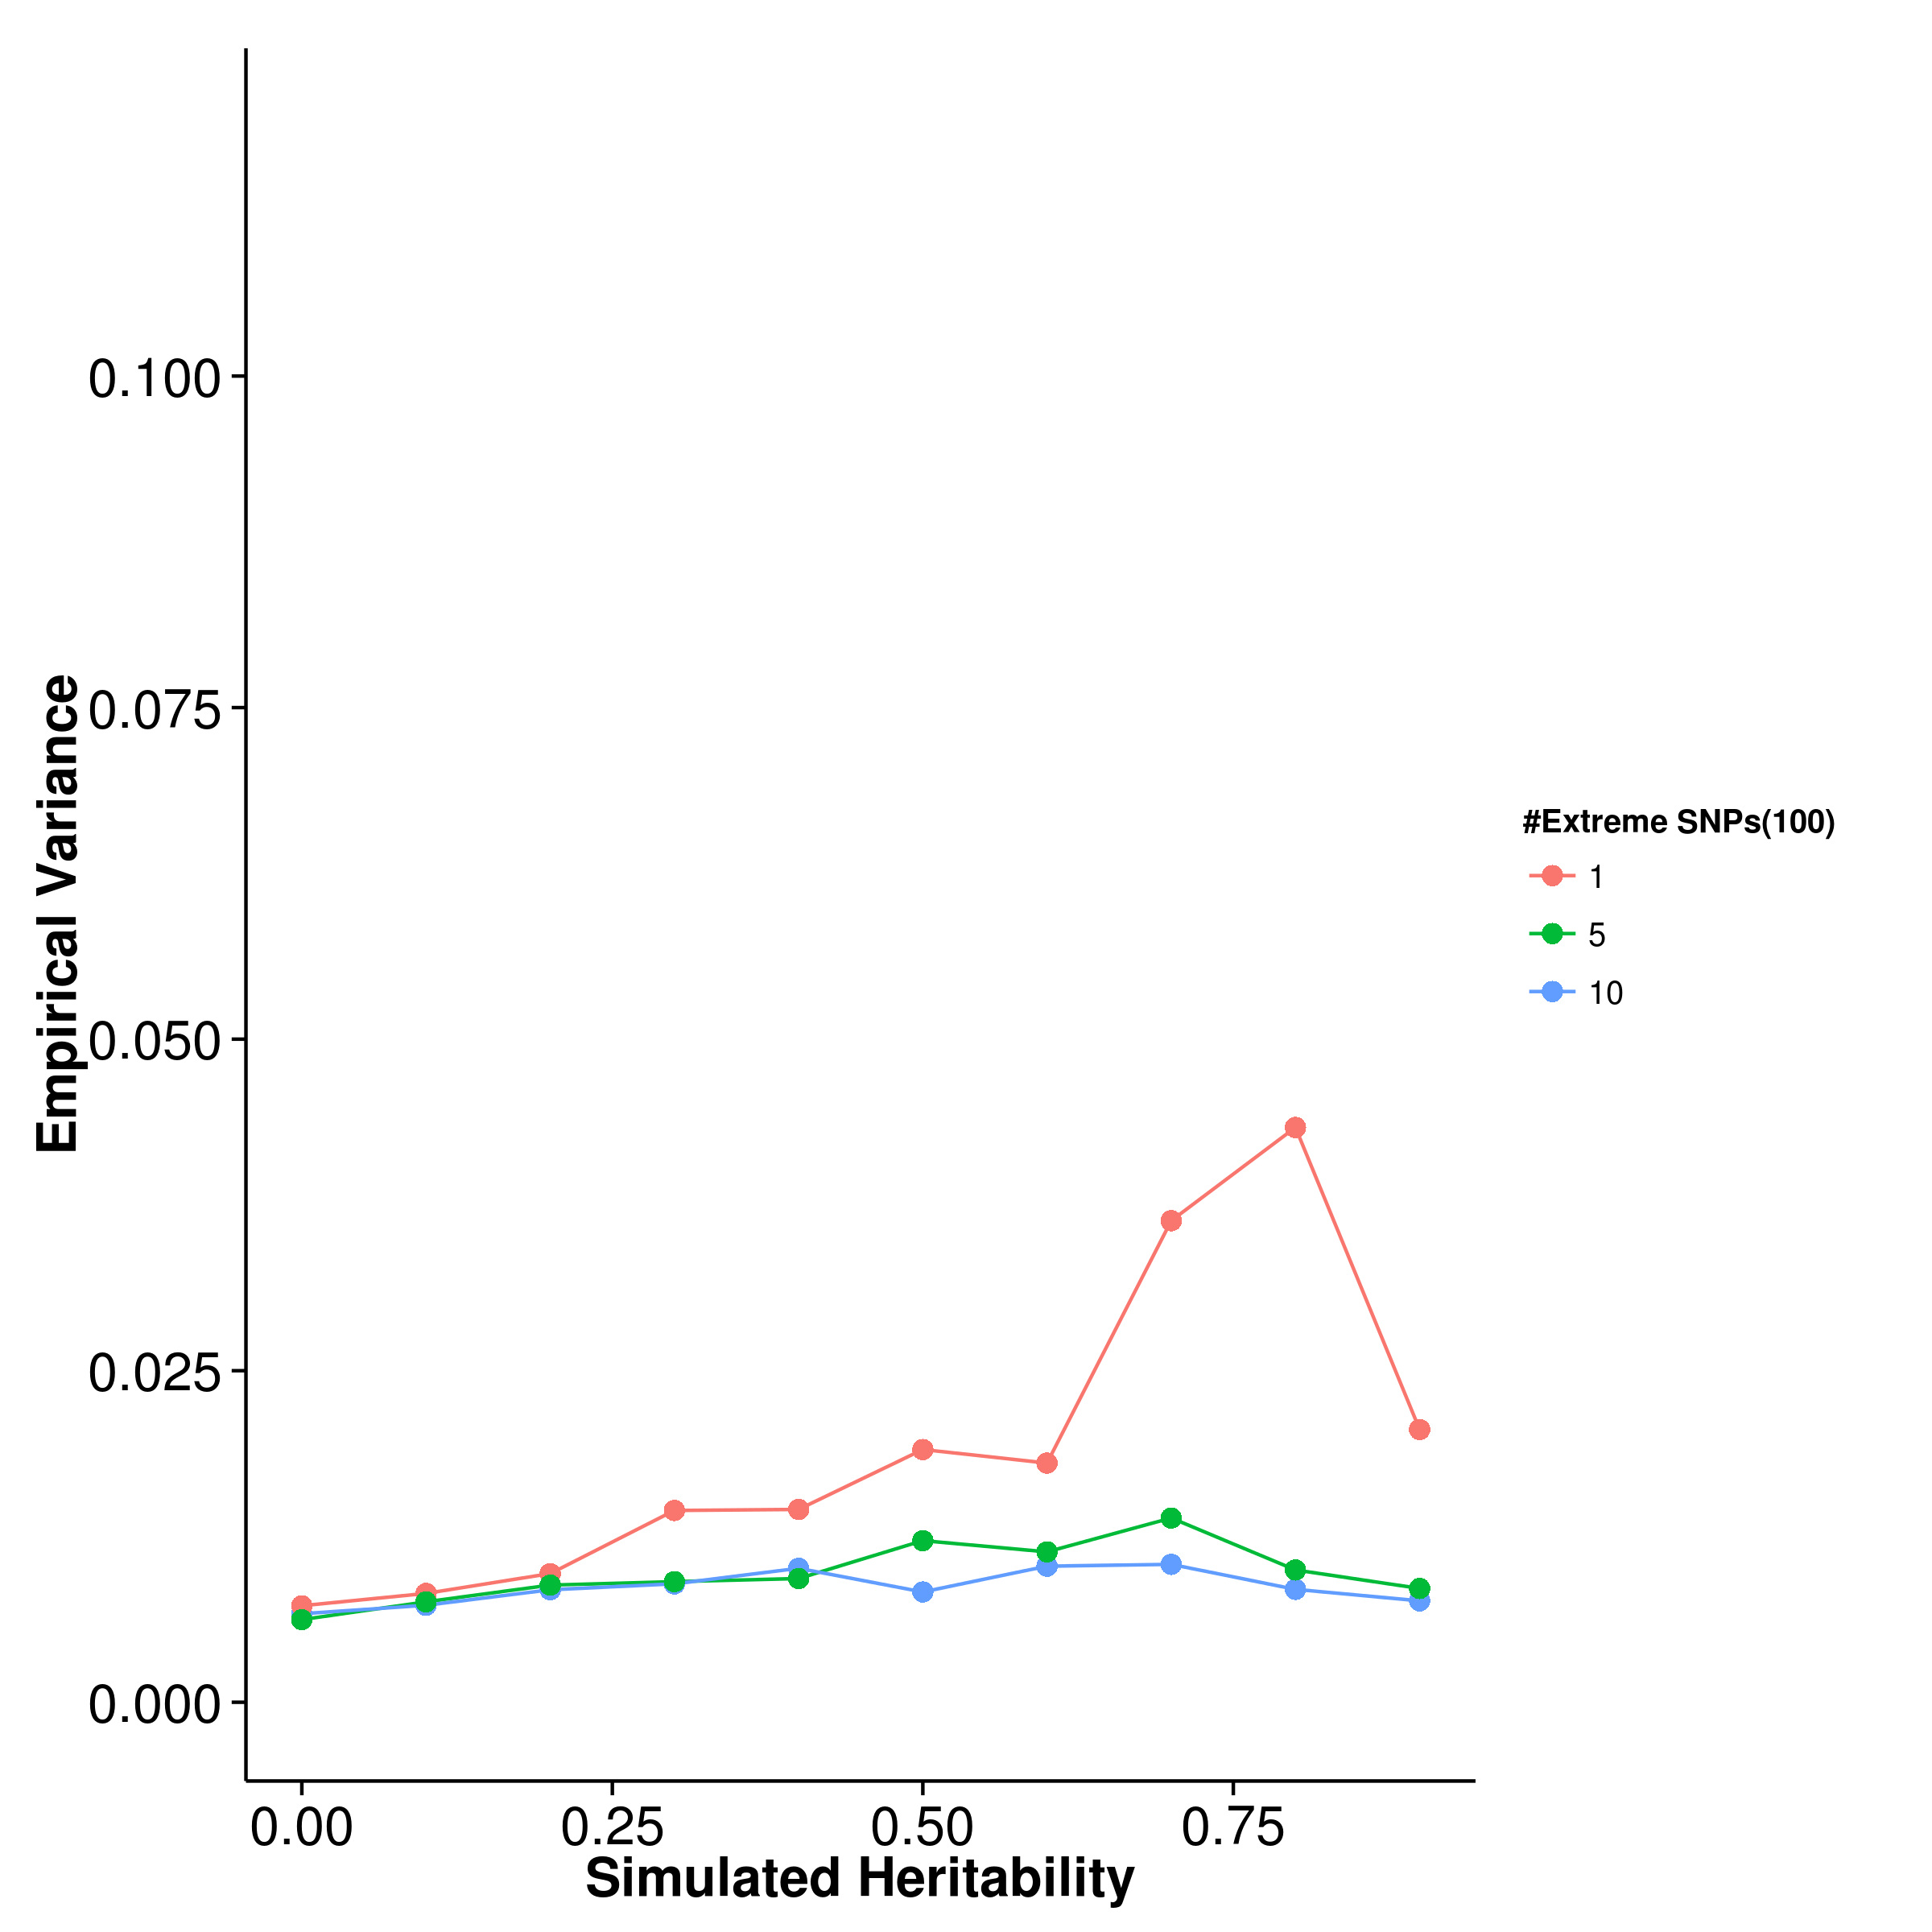
\includegraphics{figure/he_summary/extreme_100c/gcta_QtE_Rand_sd.png}}
				\label{fig:gctaQtEx100cVar}
			}\\
			\subfloat[LDSC with fix intercept]{
				\scalebox{.4}{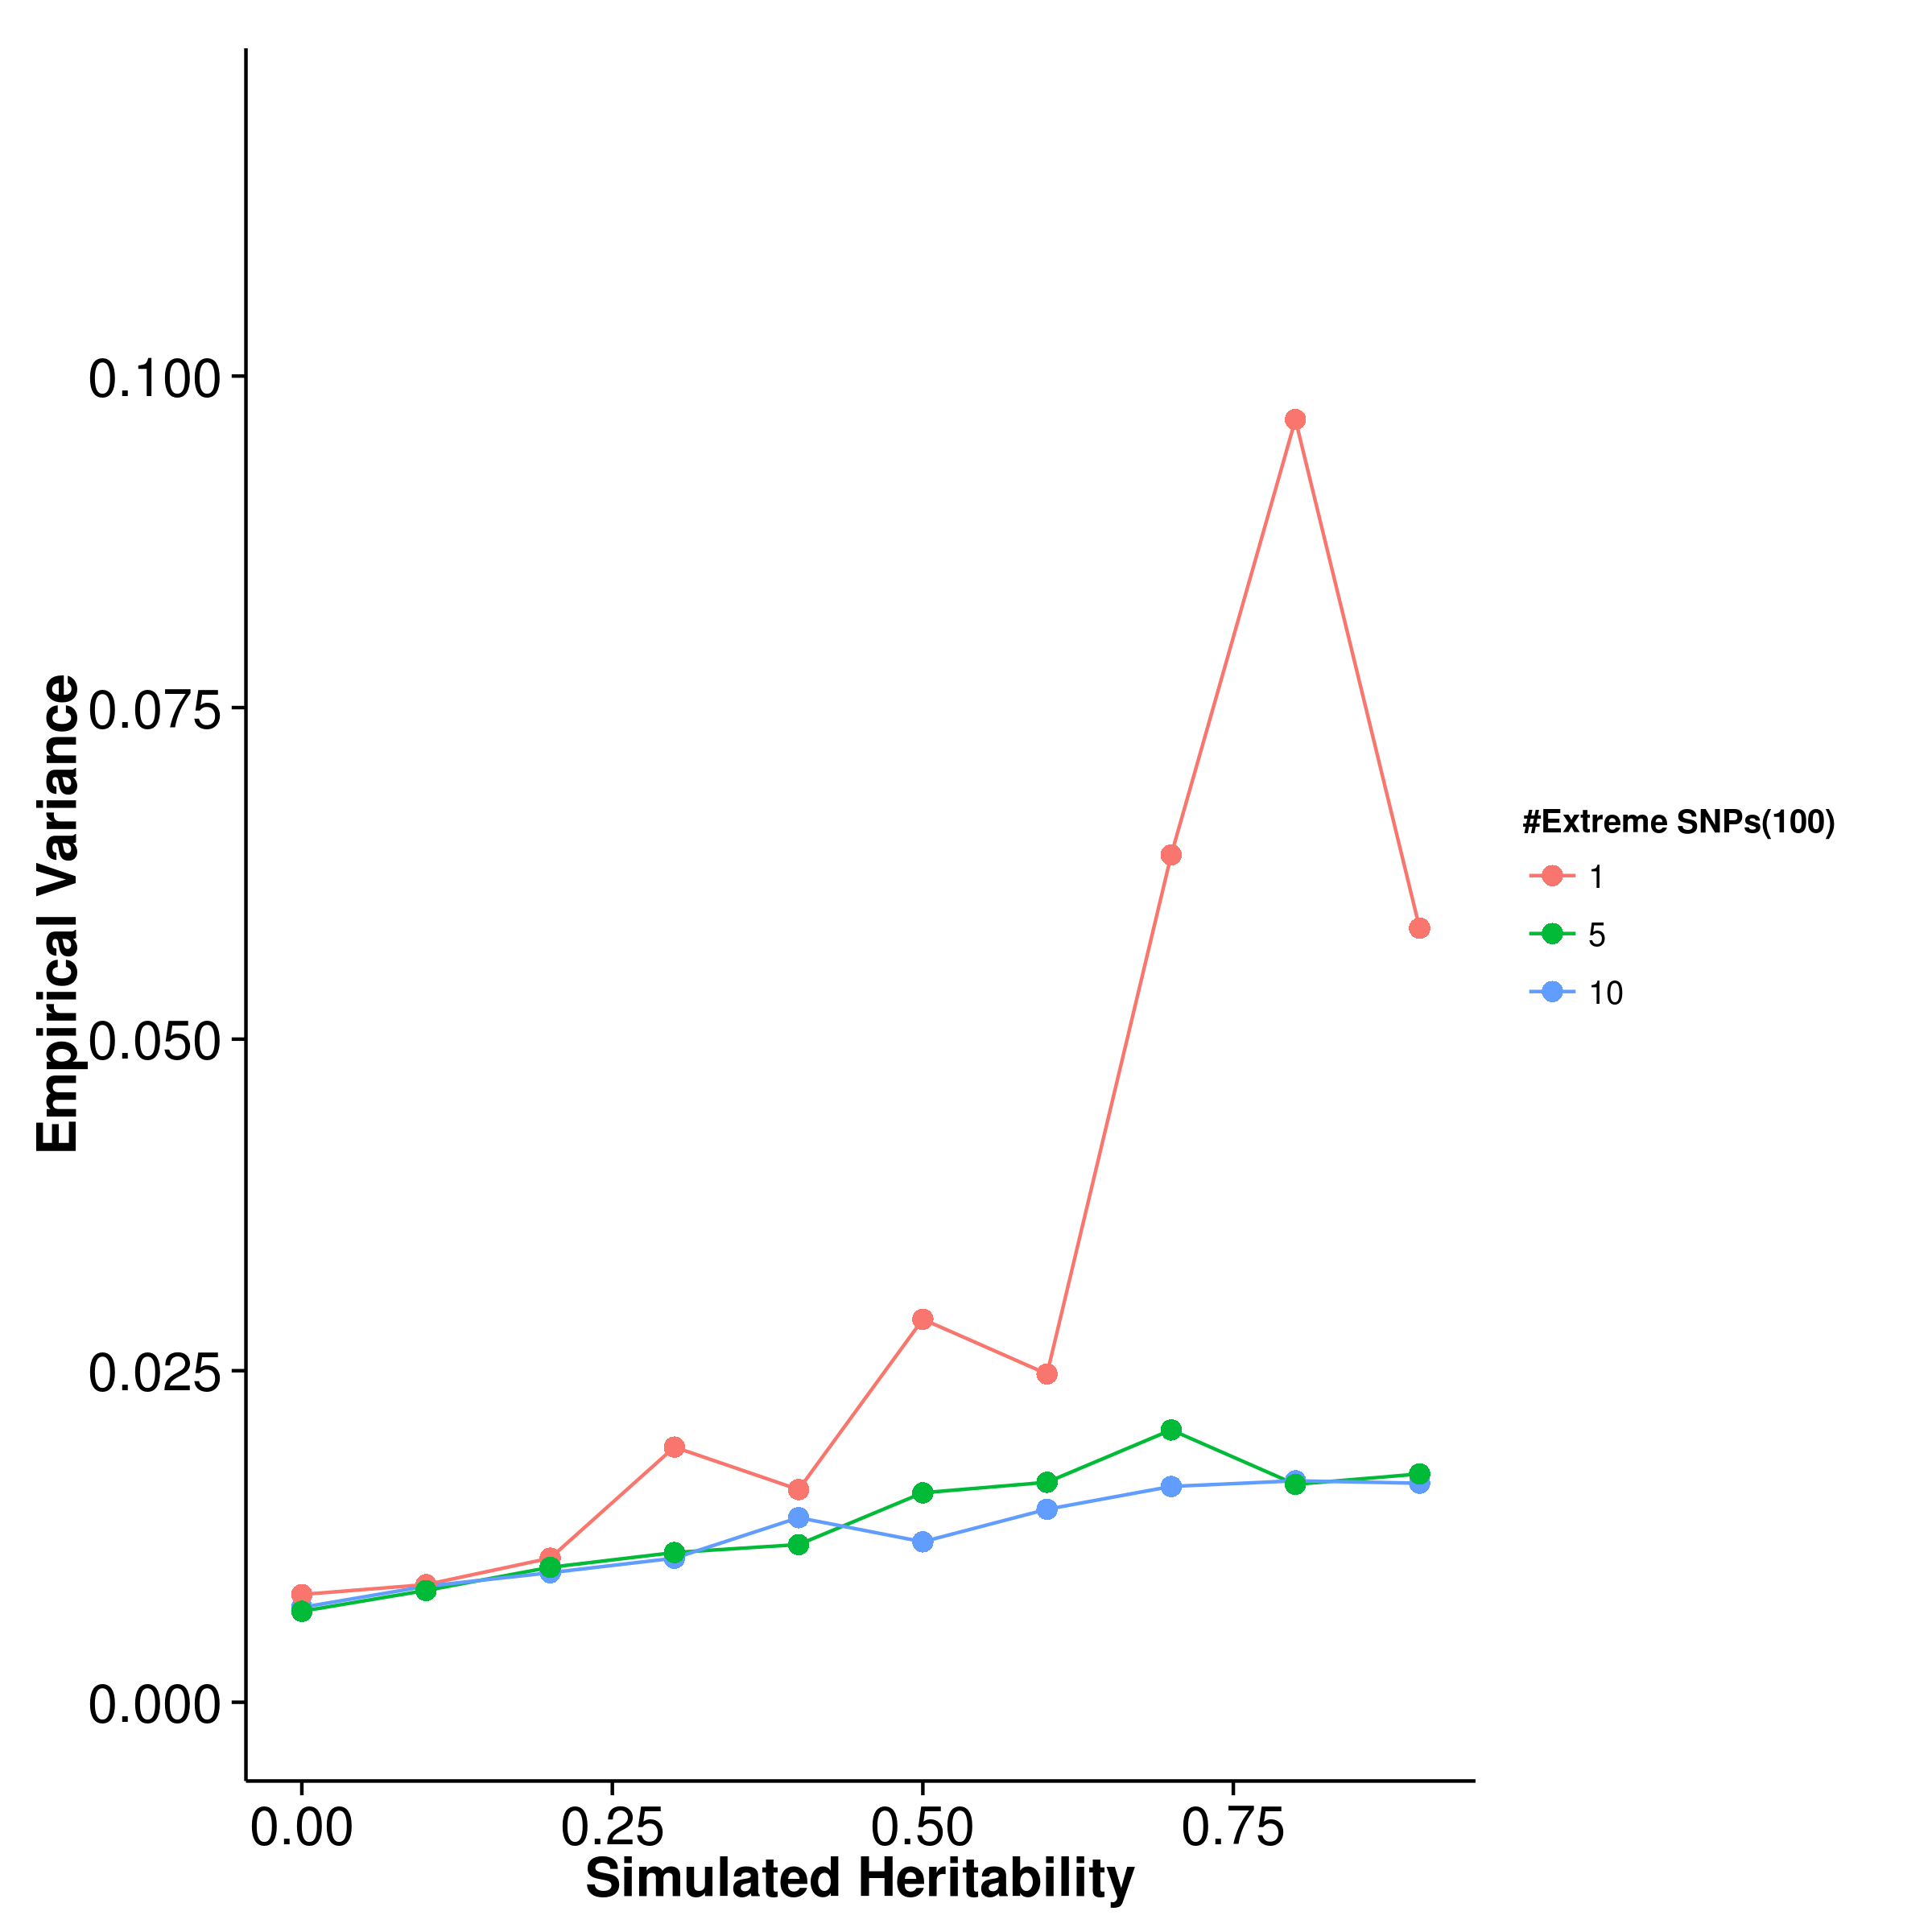
\includegraphics{figure/he_summary/extreme_100c/ldsc_QtE_Rand_sd.png}}
				\label{fig:ldscQtEx100cVar}
			}
			\subfloat[LDSC with intercept estimation]{
				
				\scalebox{.4}{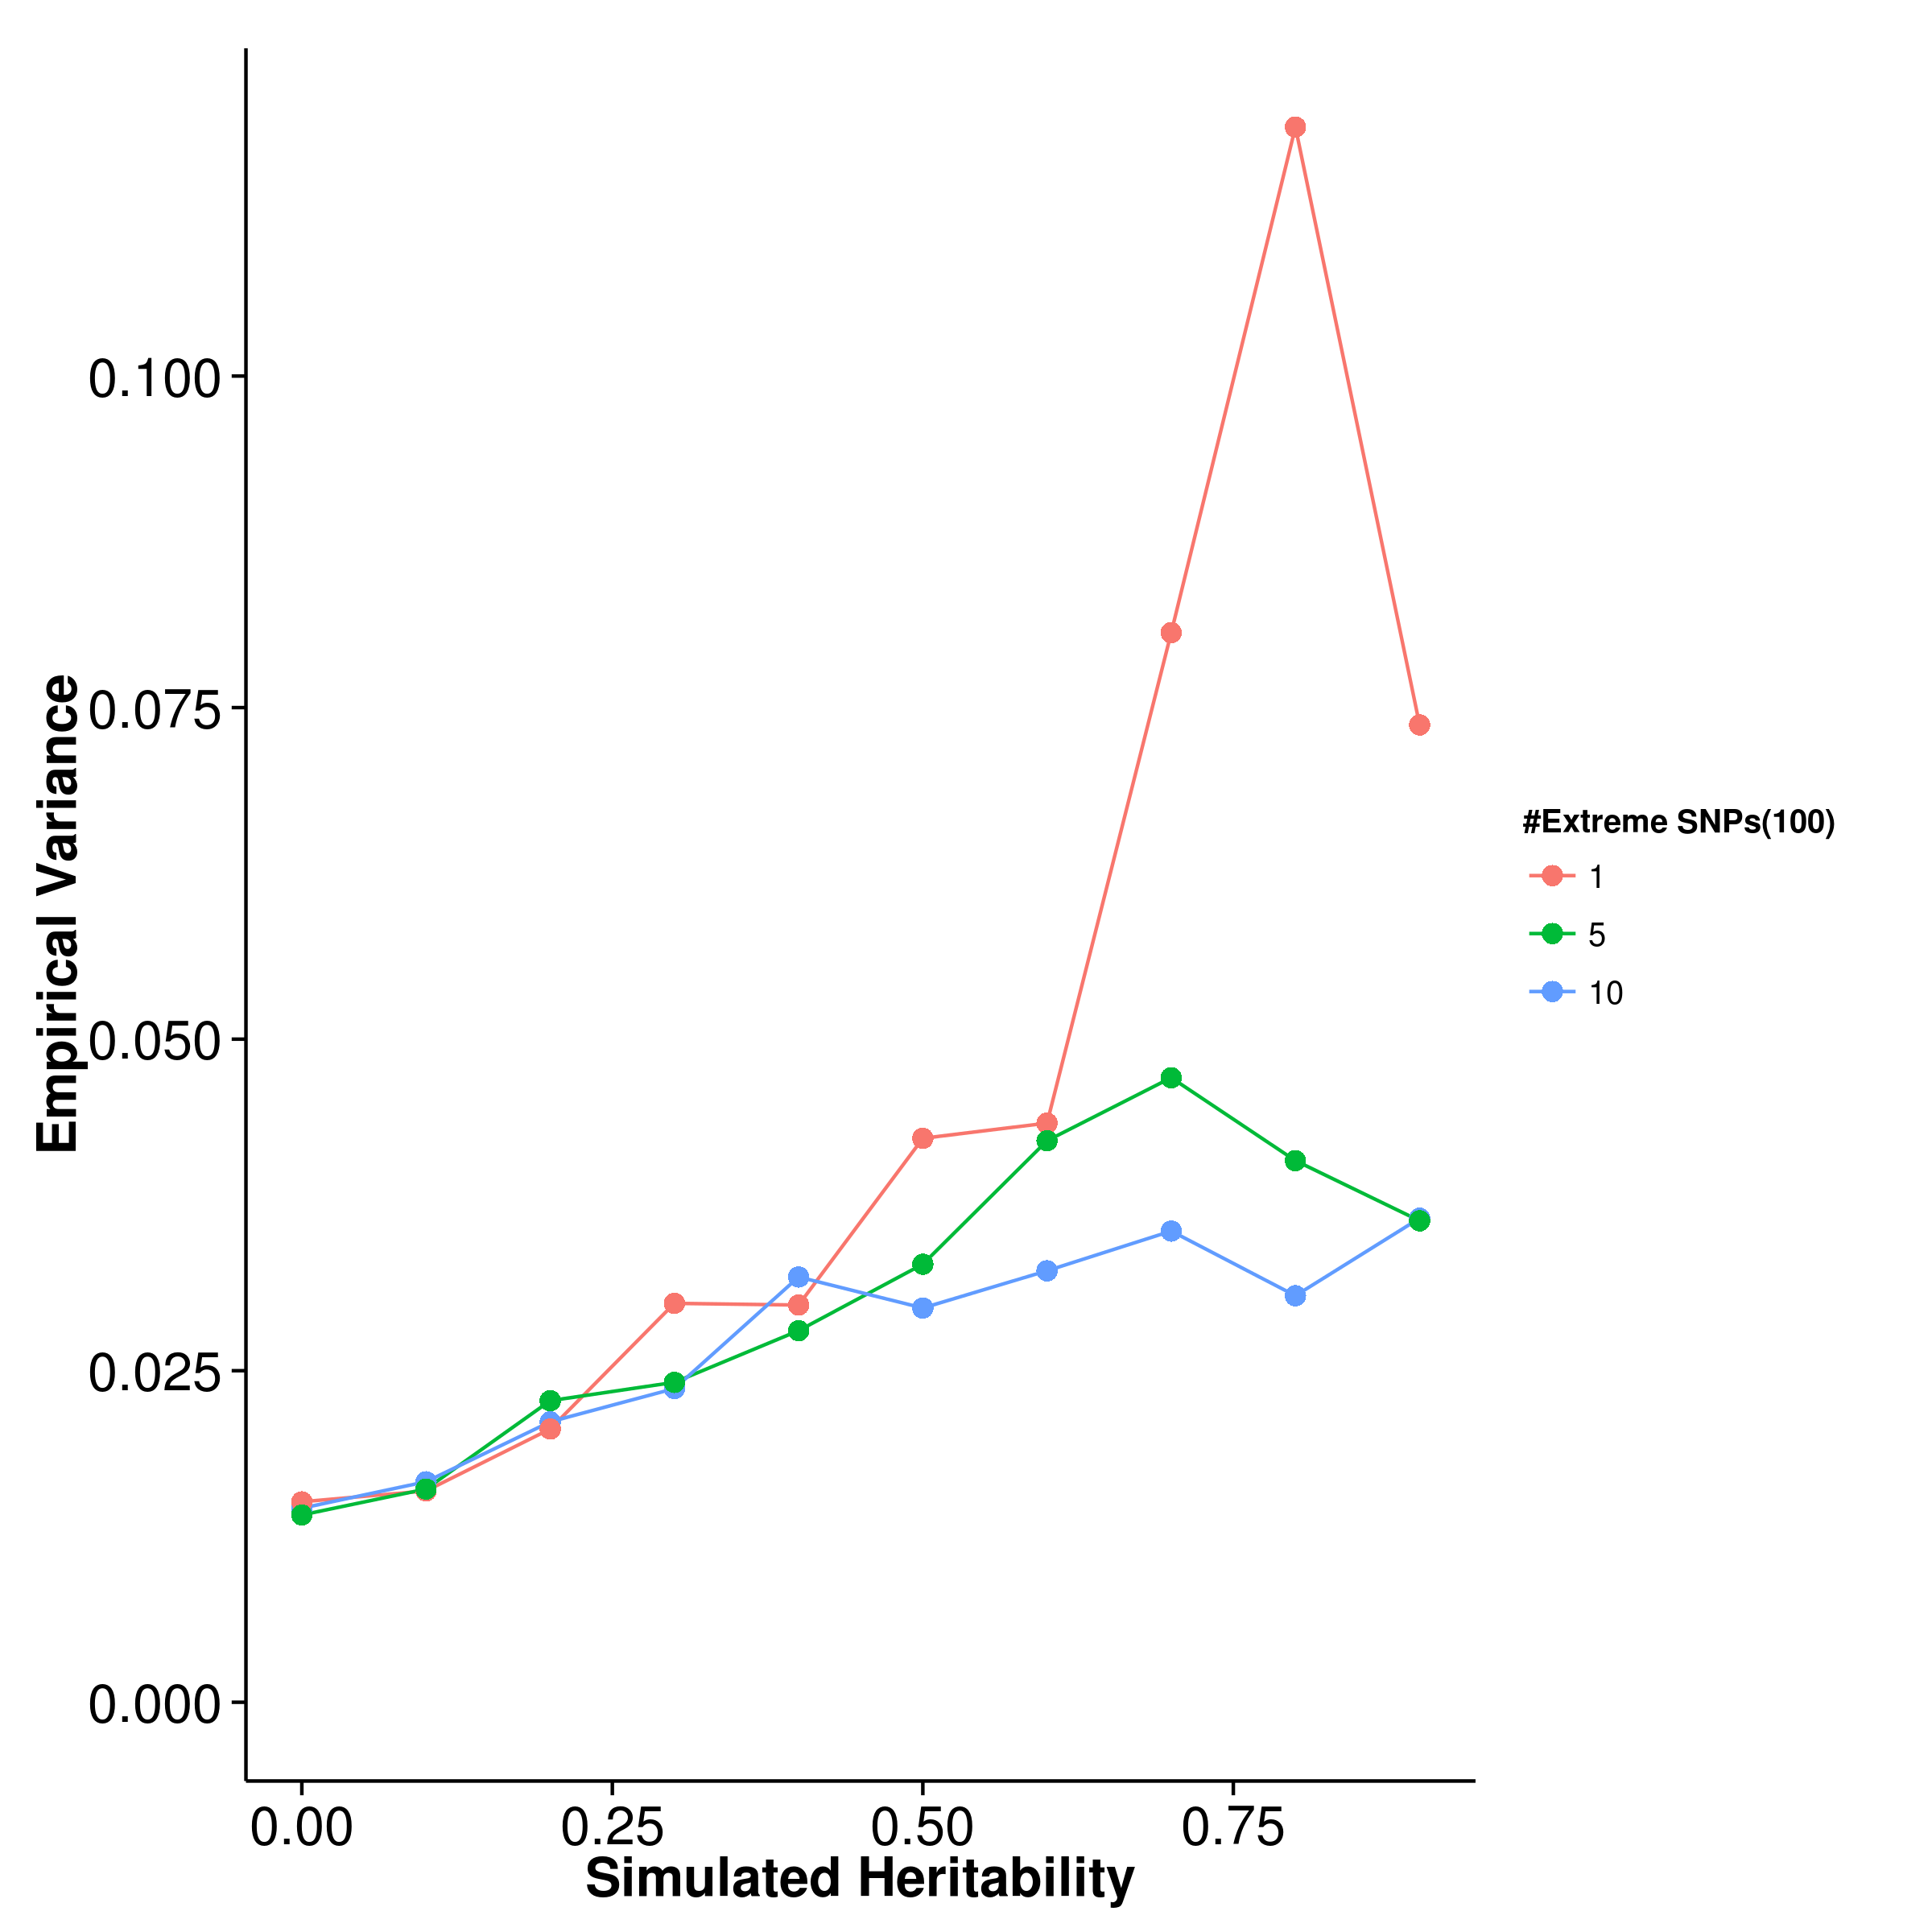
\includegraphics{figure/he_summary/extreme_100c/ldscIn_QtE_Rand_sd.png}}
				\label{fig:ldscInQtEx100cVar}
			}
			\caption[Variance of Extreme Effect Size Simulation Result]
			{Variance of results from quantitative trait simulation with extreme effect size simulation.
				100 causal \glspl{SNP} were simulated.
				When only 1 \gls{SNP} with extreme effect was simulated, the empirical variance of \gls{gcta} and \gls{ldsc} increases and a large fluctuation was observed.
				Whereas the empirical variance of \gls{shrek} only increase slightly when the simulated heritability is large and with only 1 \gls{SNP} with extreme effect.
				Suggesting that it is more robust to the change in number of extreme \gls{SNP}(s).
			} 
			\label{fig:QtEx100cVar}
		\end{figure}
		
		\begin{figure}
			\centering
			\subfloat[SHREK]{
				\scalebox{.4}{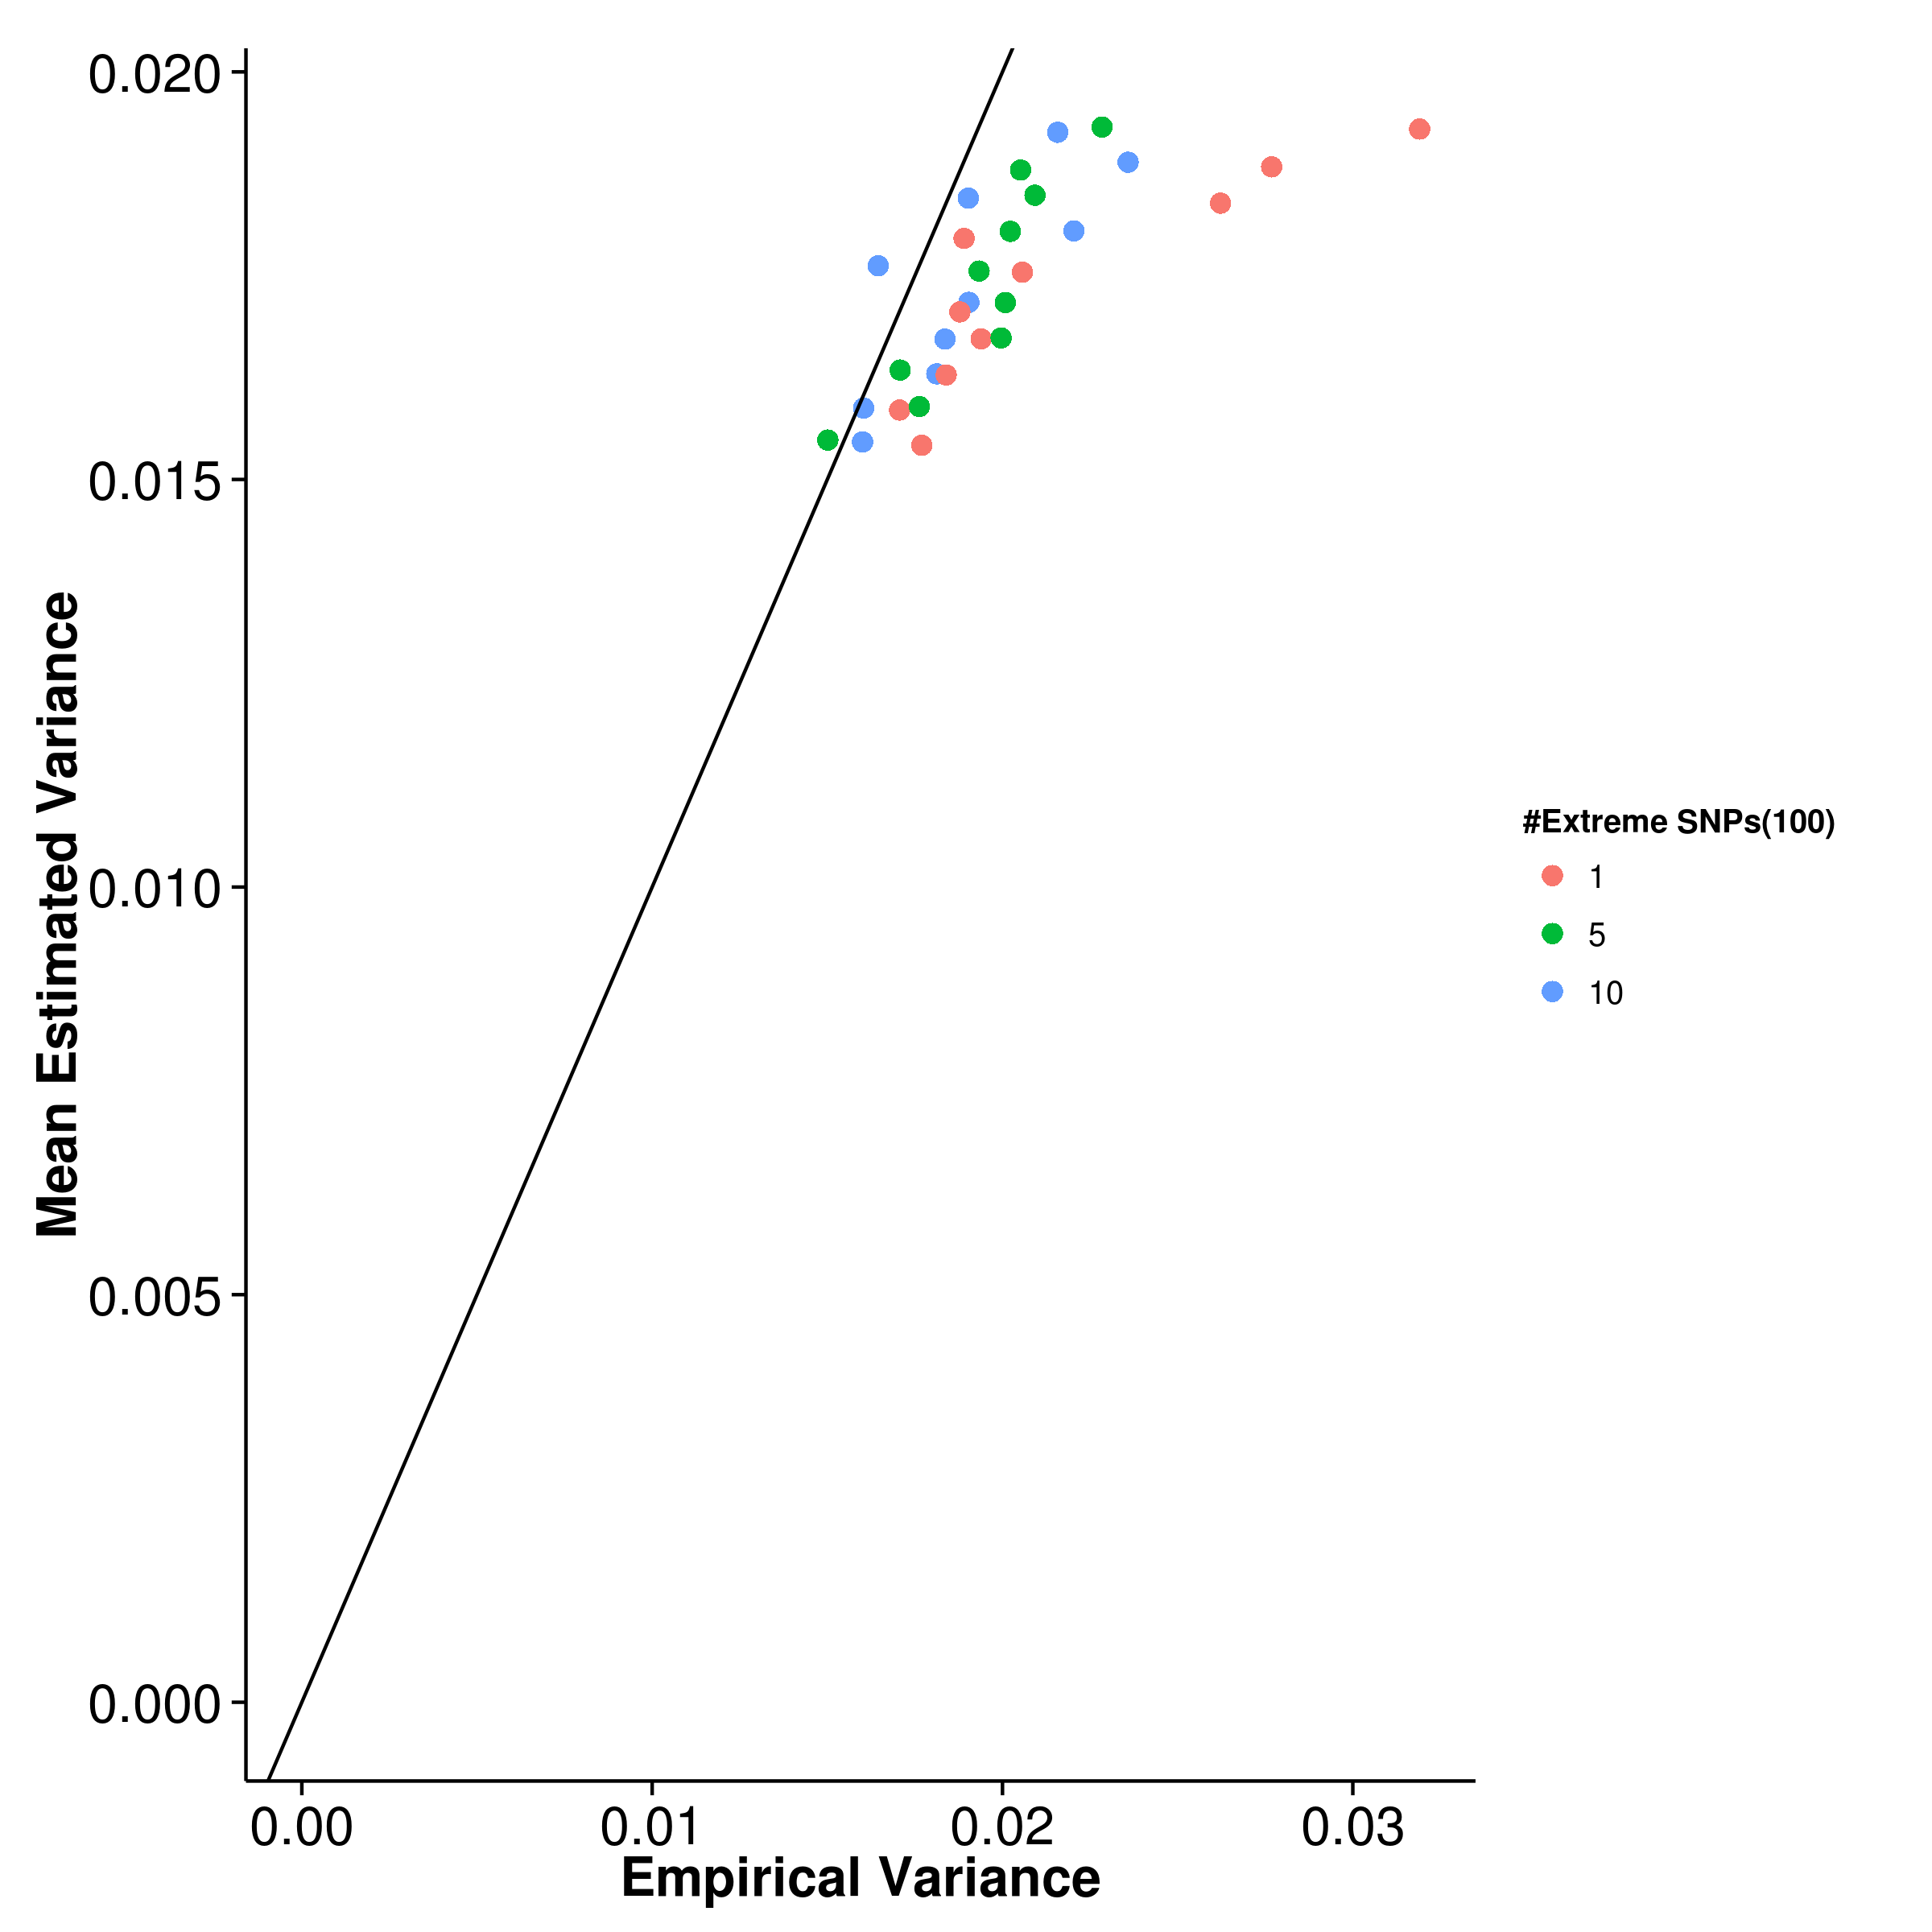
\includegraphics{figure/he_summary/extreme_100c/shrek_QtE_Rand_sdCom.png}}
				\label{fig:shrekQtEx100cVarCom}
			}
			\subfloat[GCTA]{
				\scalebox{.4}{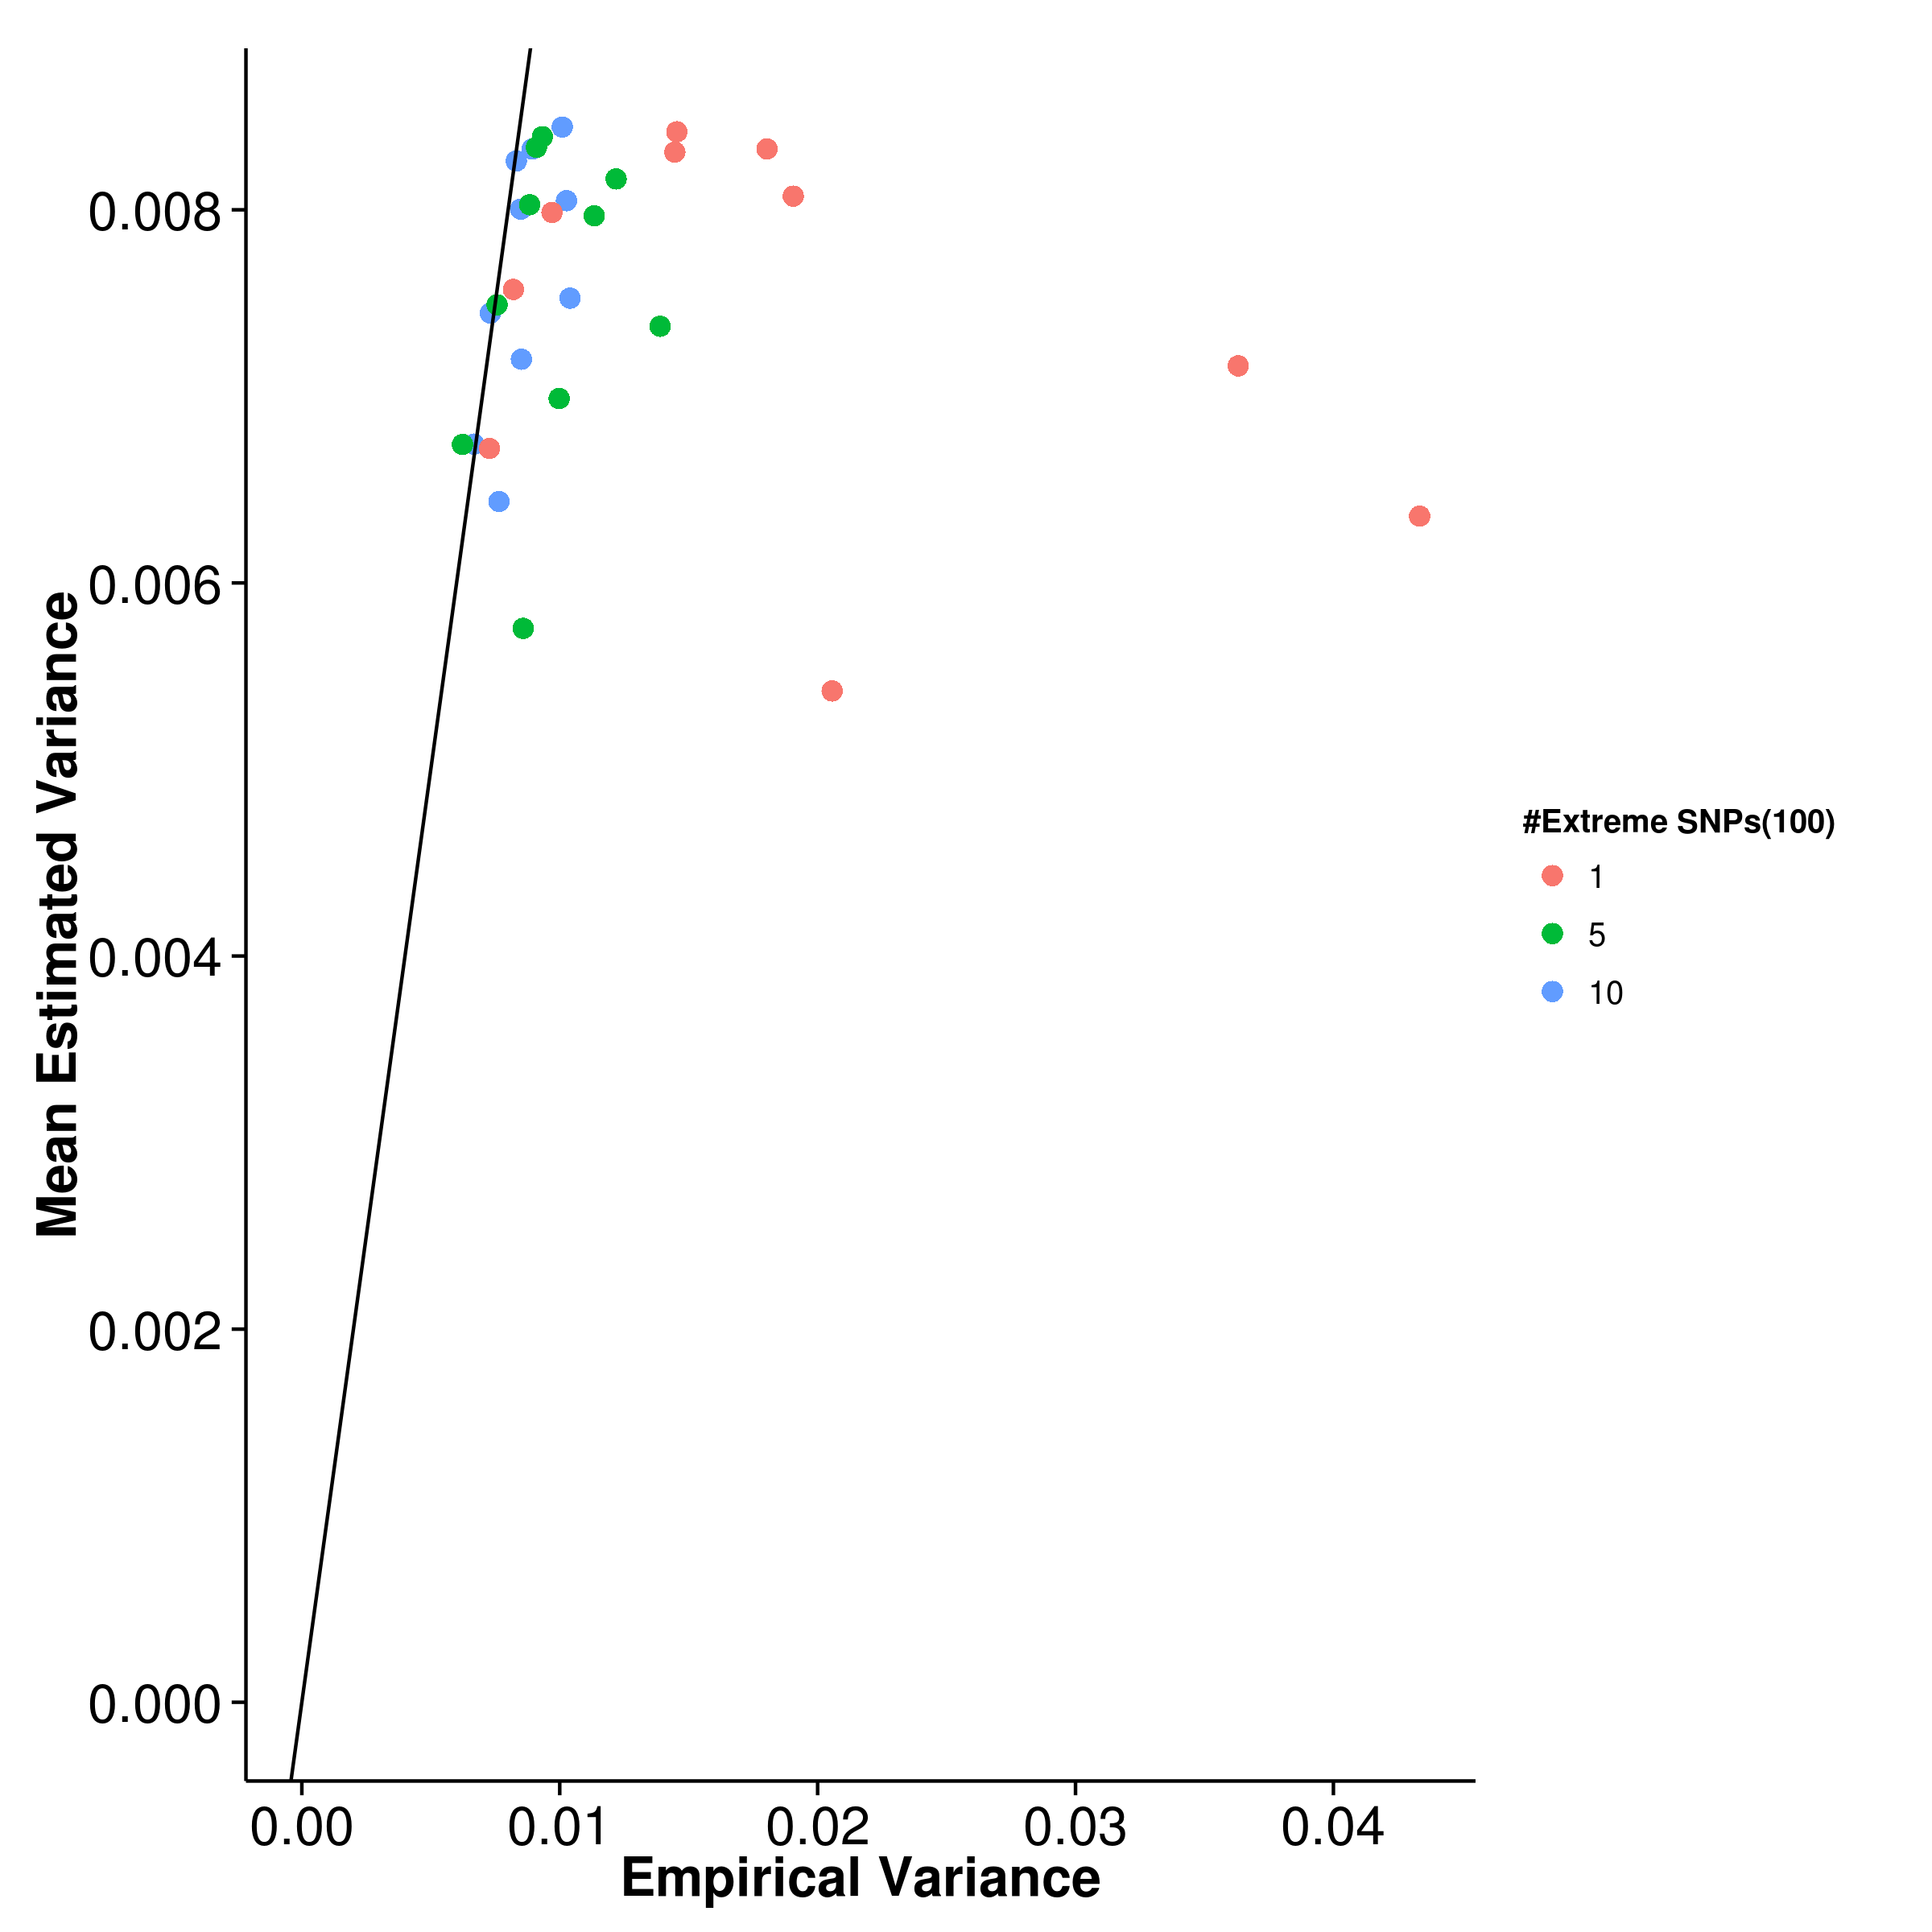
\includegraphics{figure/he_summary/extreme_100c/gcta_QtE_Rand_sdCom.png}}
				\label{fig:gctaQtEx100cVarCom}
			}\\
			\subfloat[LDSC with fix intercept]{
				\scalebox{.4}{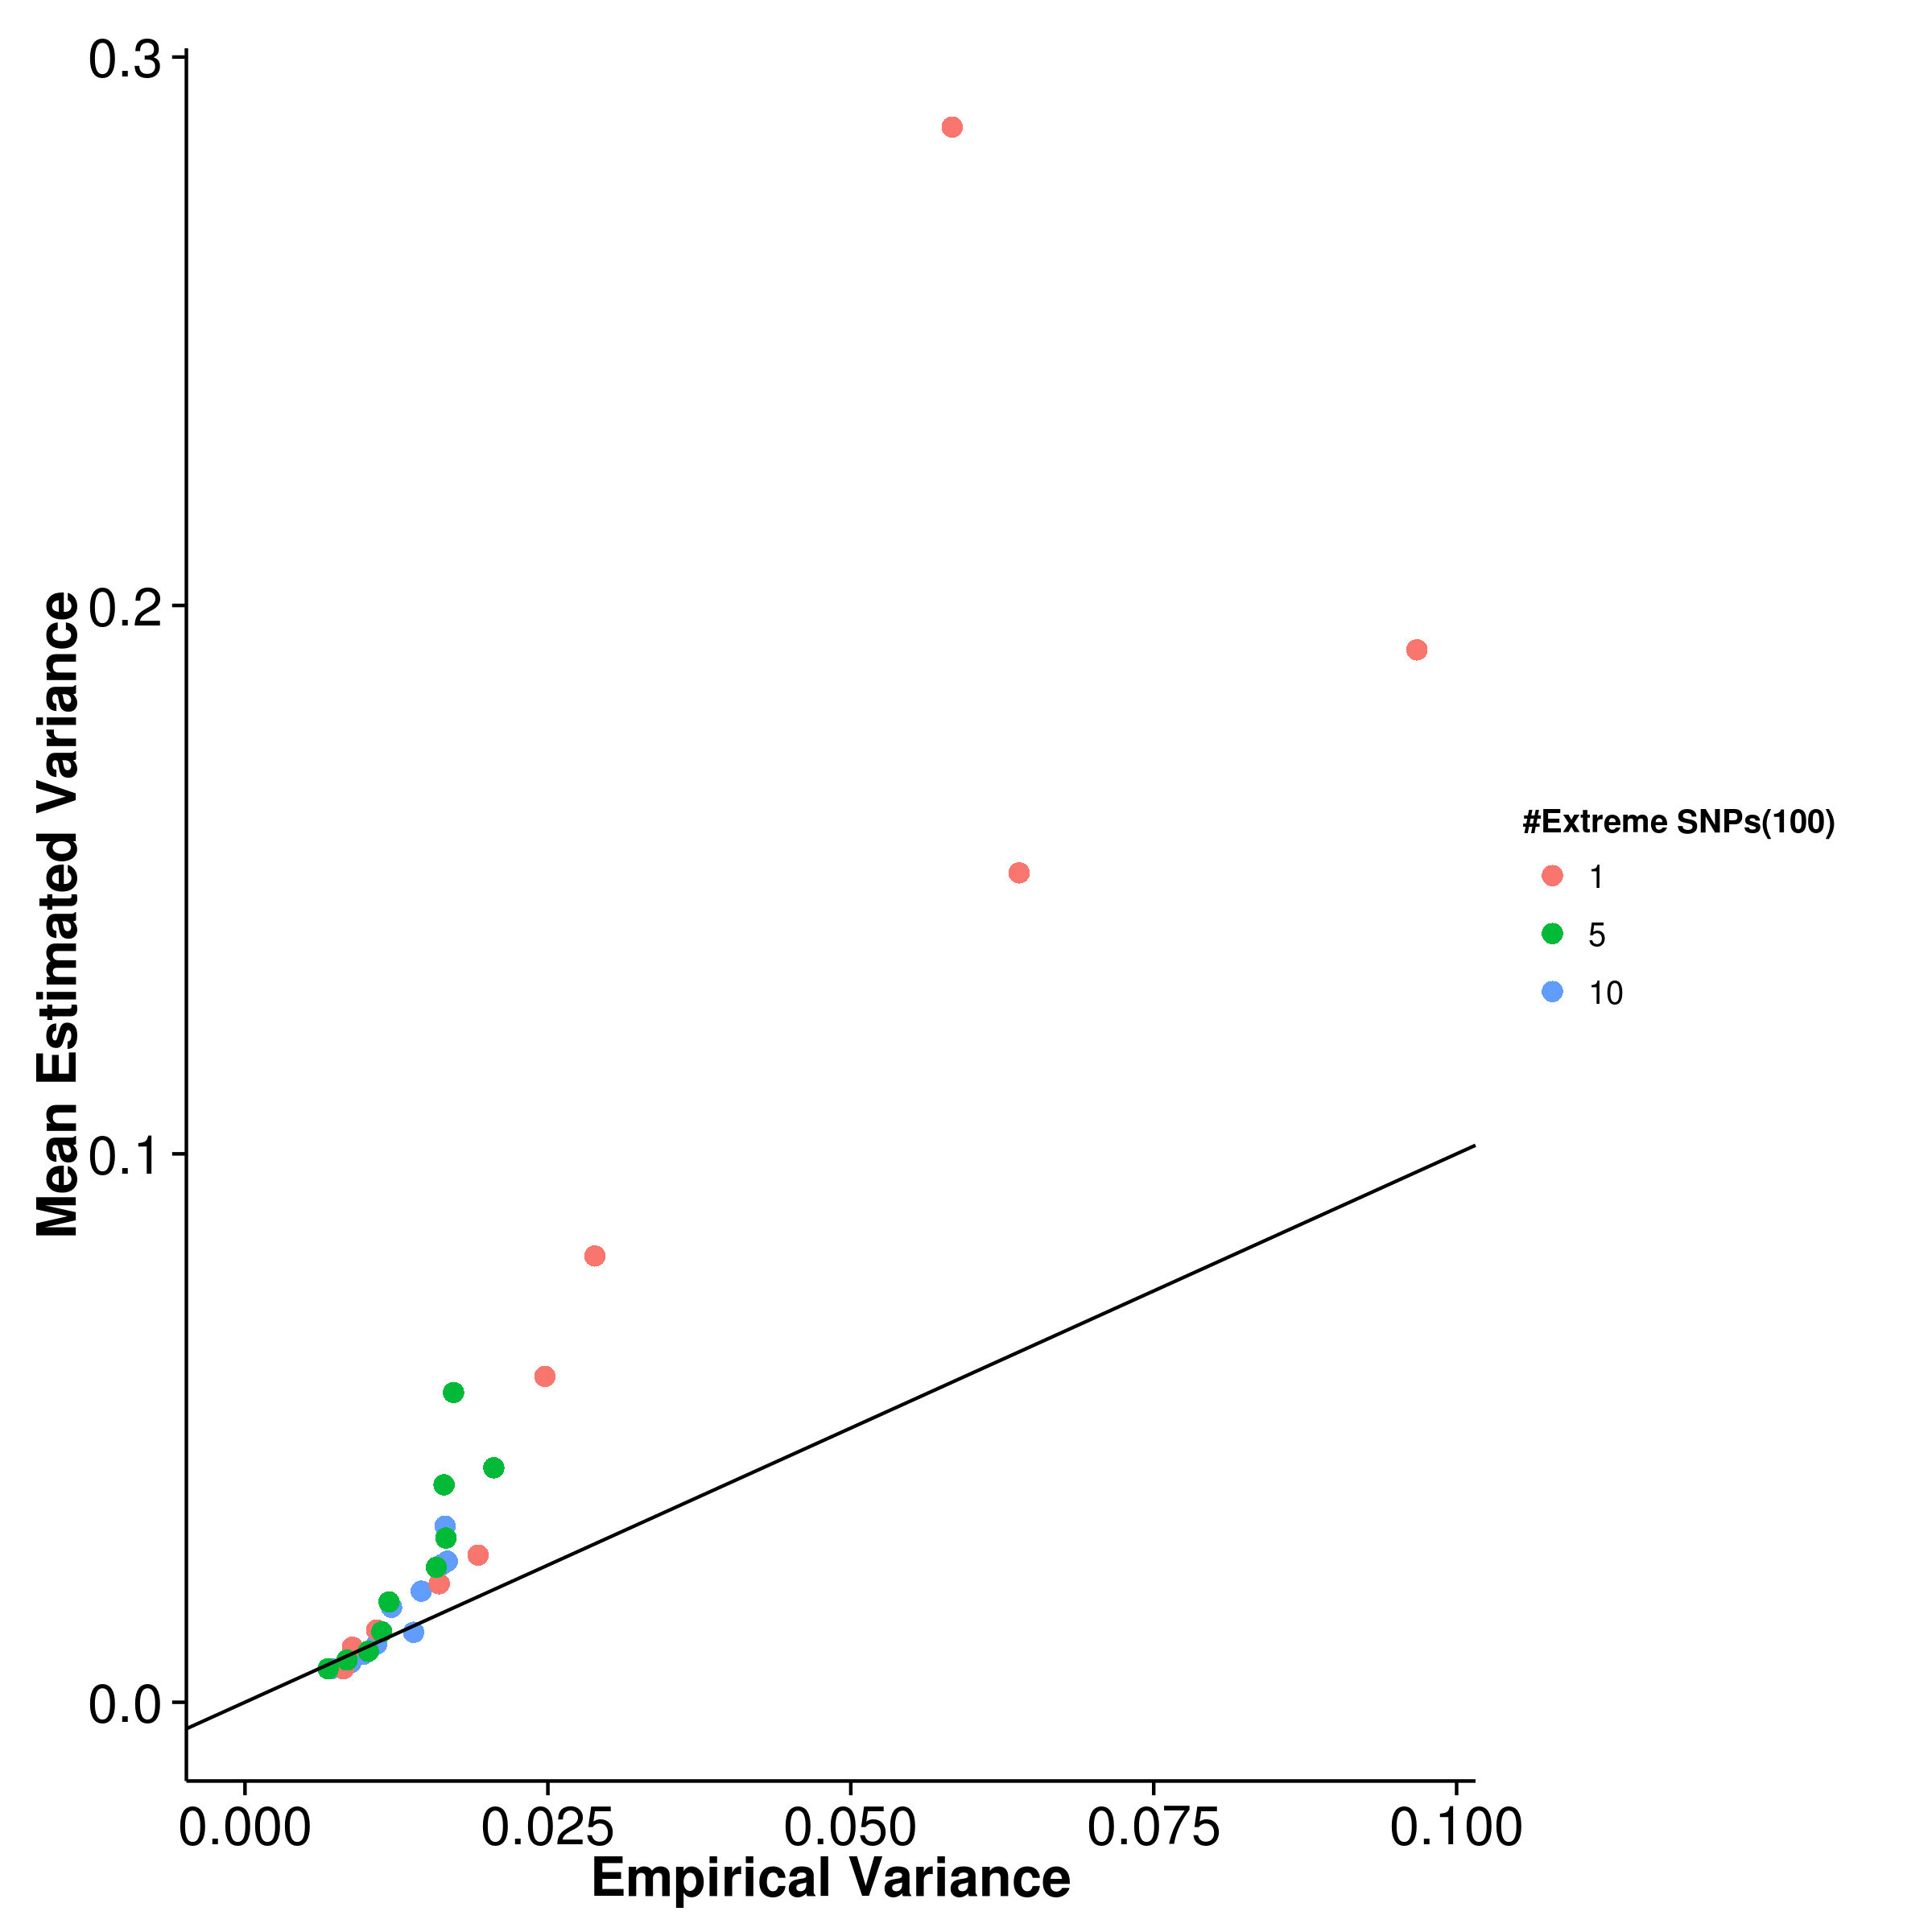
\includegraphics{figure/he_summary/extreme_100c/ldsc_QtE_Rand_sdCom.png}}
				\label{fig:ldscQtEx100cVarCom}
			}
			\subfloat[LDSC with intercept estimation]{
				
				\scalebox{.4}{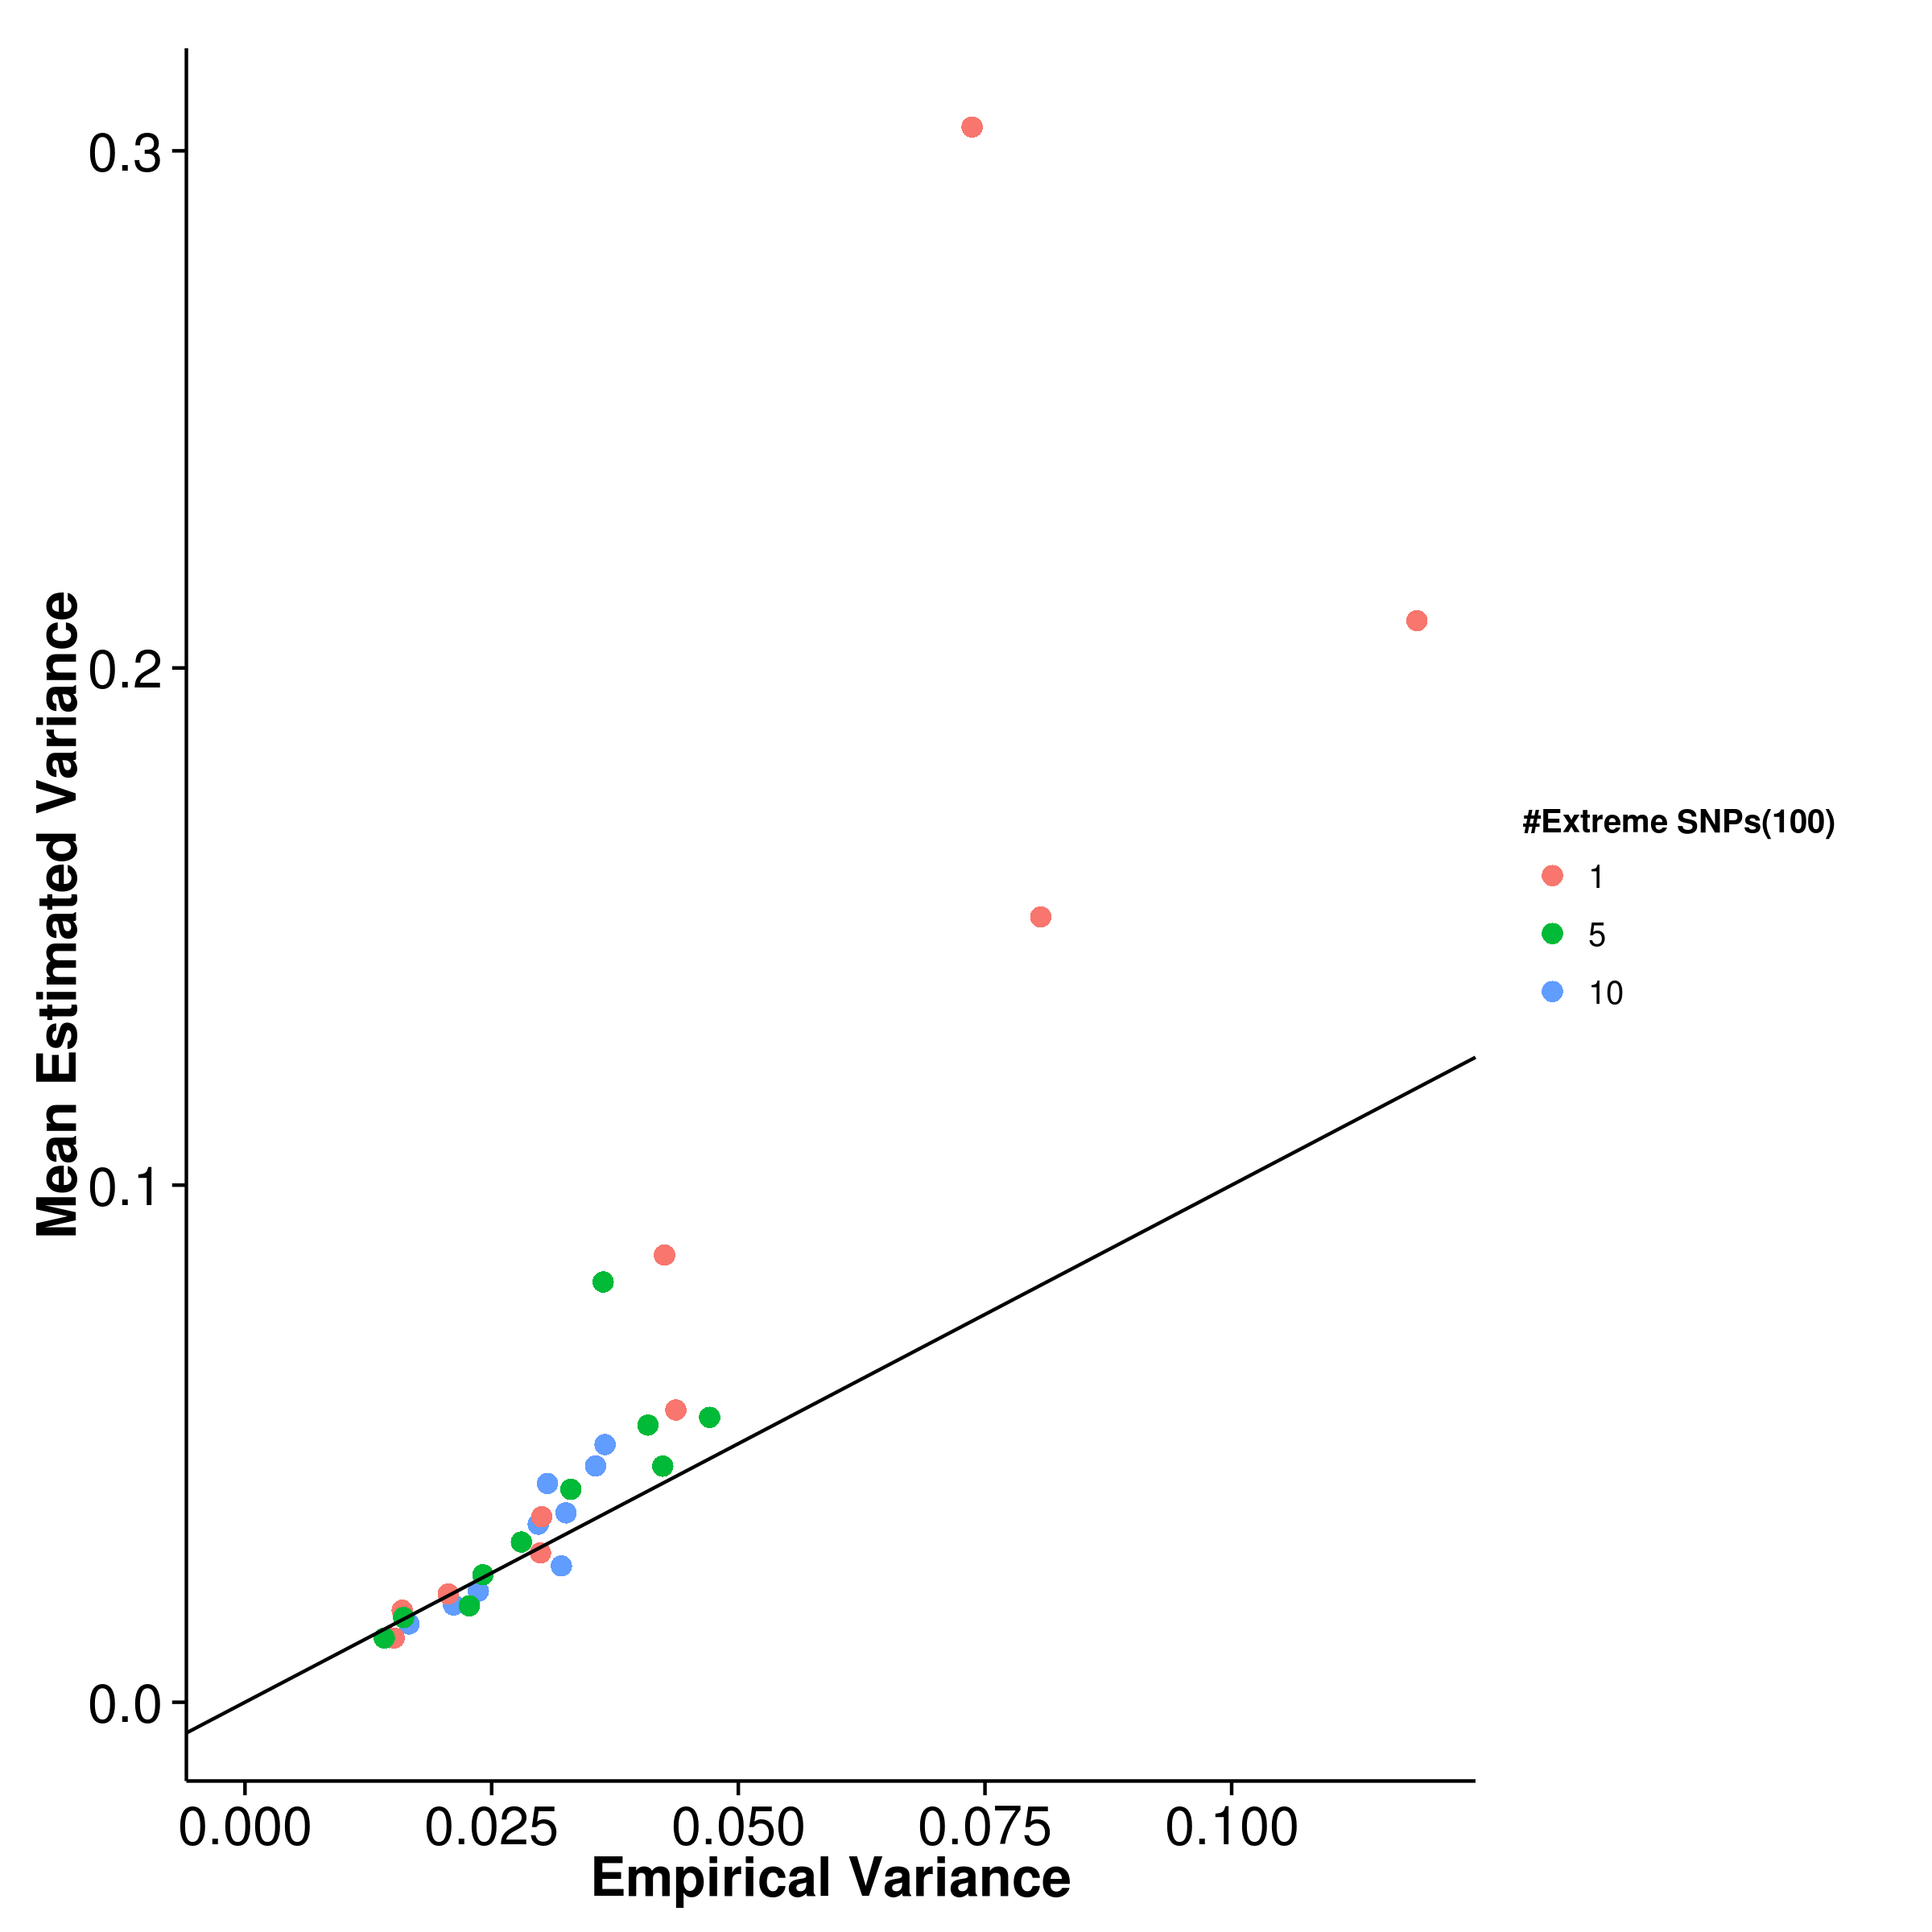
\includegraphics{figure/he_summary/extreme_100c/ldscIn_QtE_Rand_sdCom.png}}
				\label{fig:ldscInQtEx100cVarCom}
			}
			\caption[Estimation of Variance in Extreme Effect Size Simulation]
			{Estimated variance of results from quantitative trait simulation with extreme effect size simulation when compared to the empirical variance.
				100 causal \glspl{SNP} were simulated.
				\gls{shrek} and \gls{gcta} generally under-estimate the variance with the magnitude of bias being the highest when there is only 1 \gls{SNP} with extreme effect.
				On the other hand, \gls{ldsc} tends to over-estimate the variance and it can overestimate the variance by more than 3 folds when there is only 1 \gls{SNP} with extreme effect.
			} 
			\label{fig:QtEx100cVarCom}
		\end{figure}
		Another condition that we were interested in was in the case where a small portion of \glspl{SNP} has a much larger effect than other \glspl{SNP}.
		In this simulation, we simulated either 100 or 250 causal \glspl{SNP} with 1, 5 or 10 \glspl{SNP} having a much larger effect.
		
		% Extreme with 250 causal
		
		\begin{figure}
			\centering
			\subfloat[SHREK]{
				\scalebox{.4}{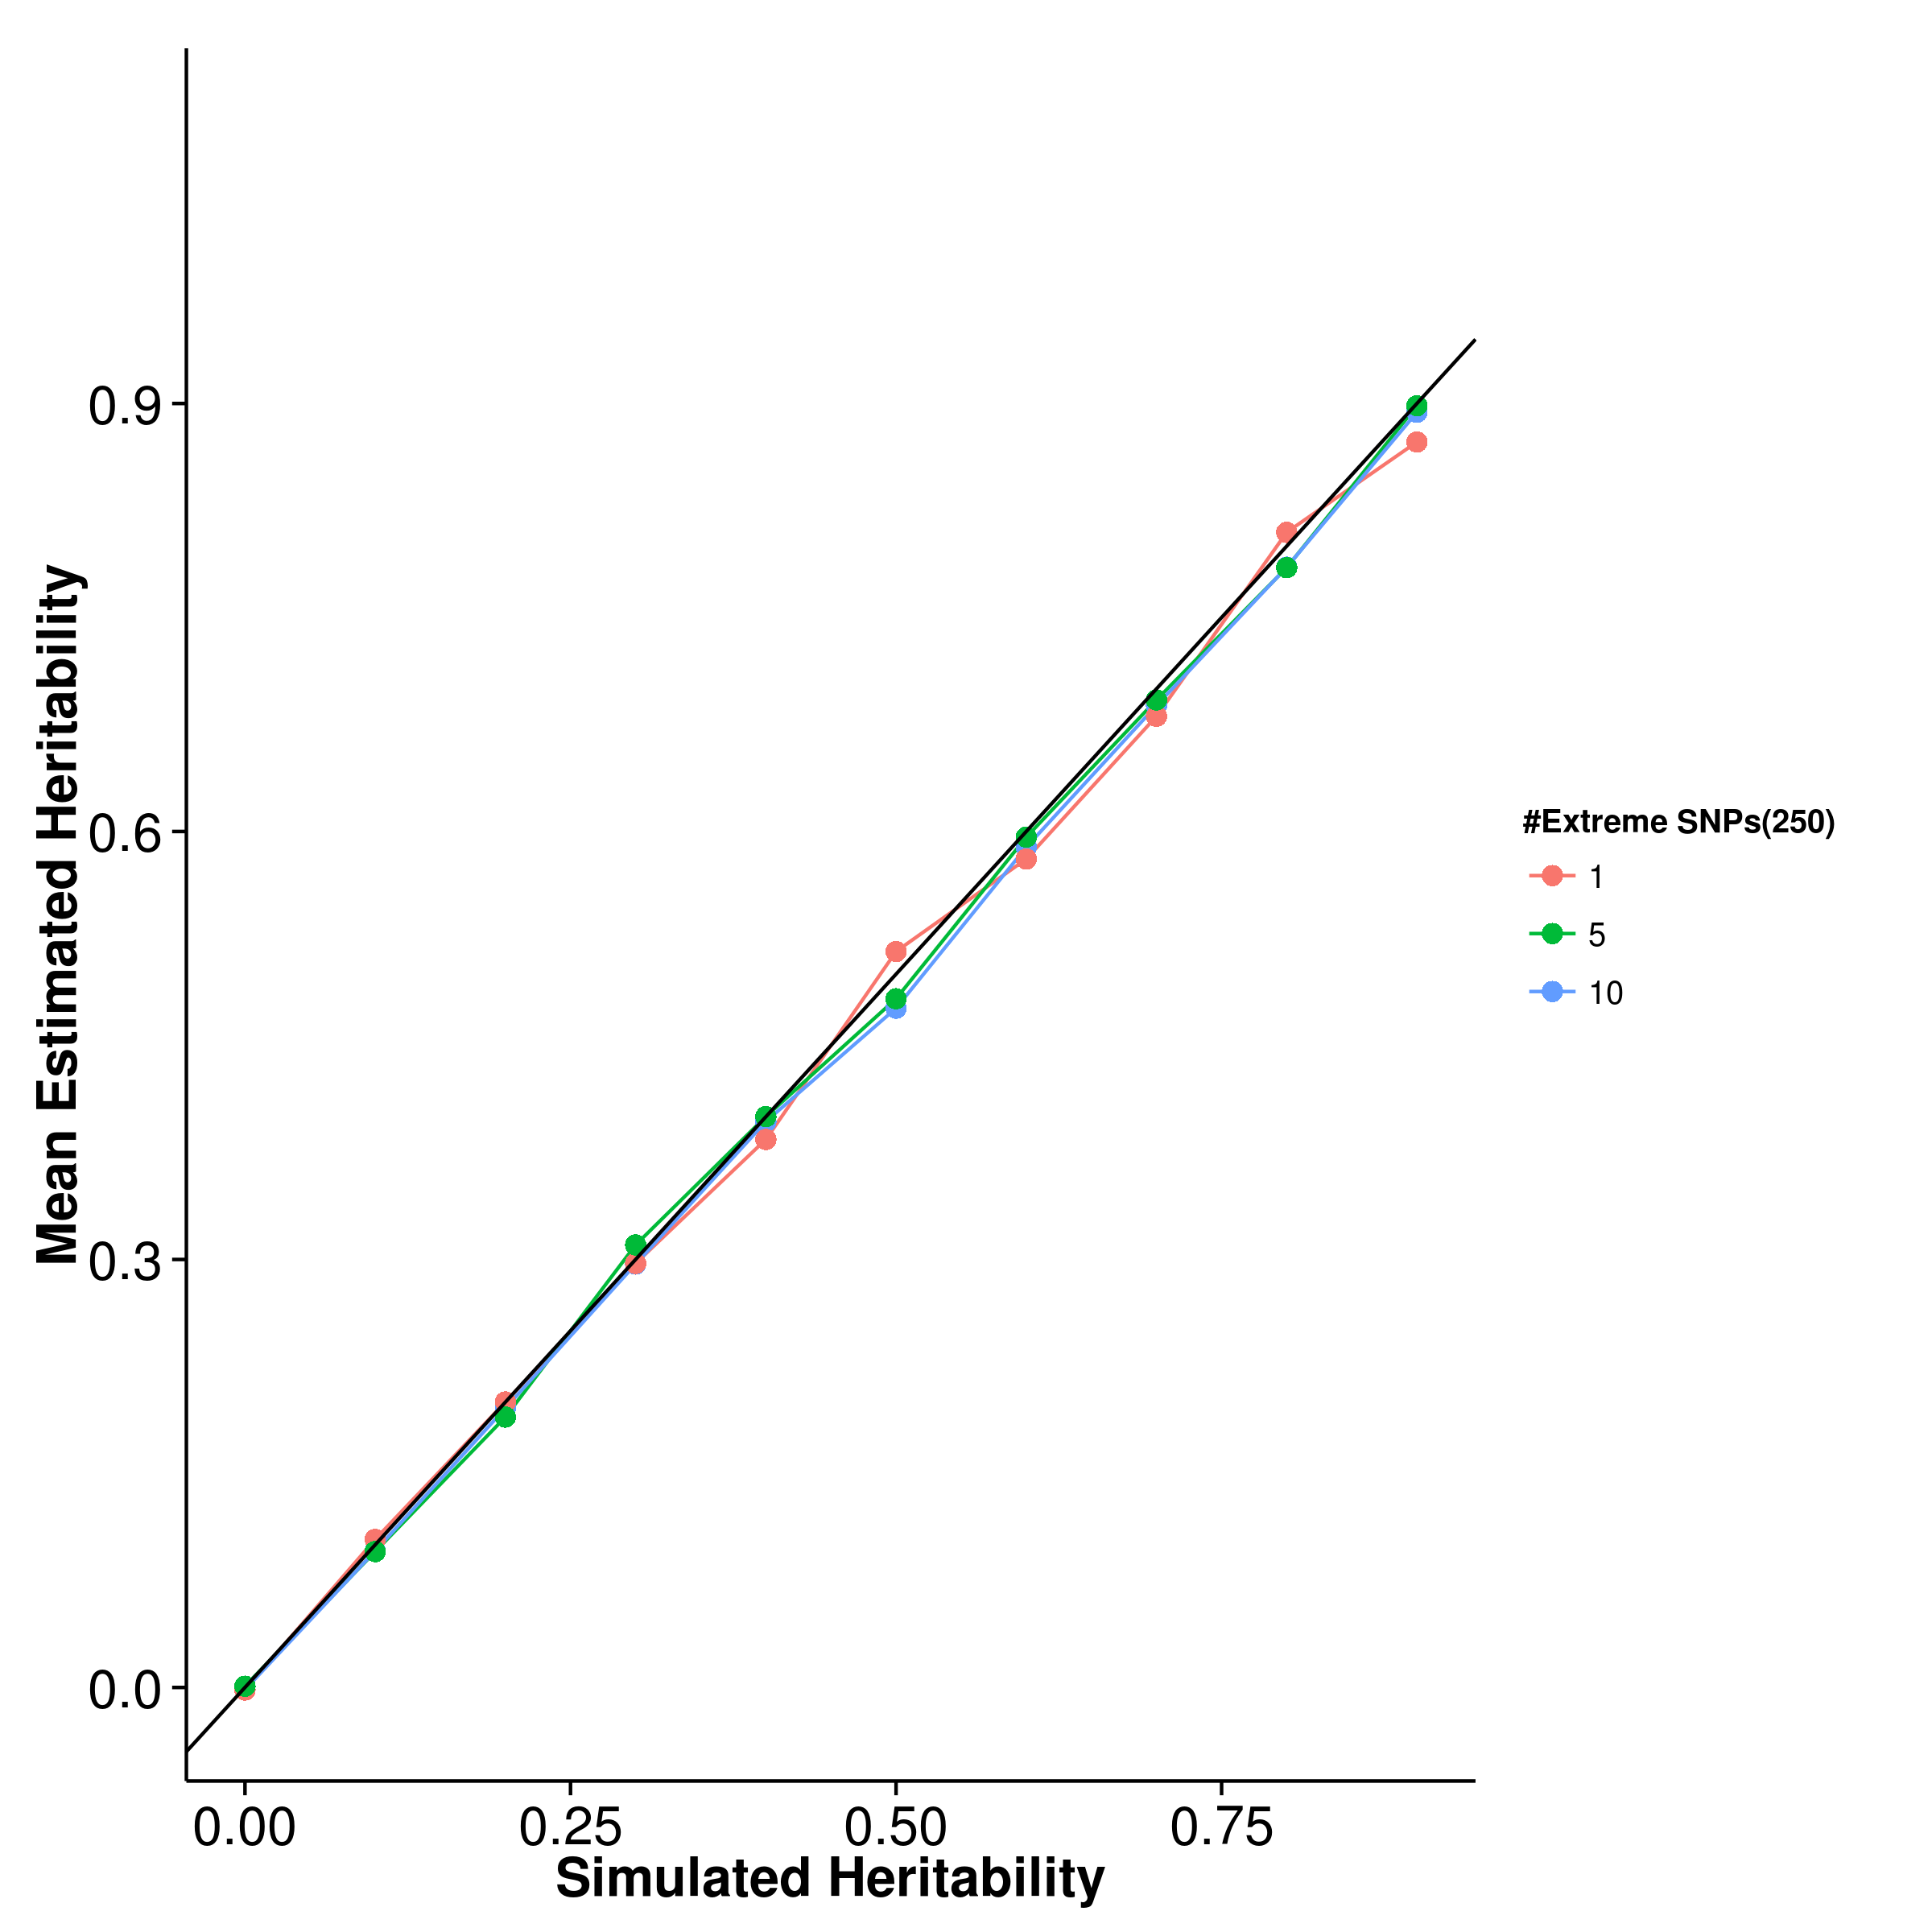
\includegraphics{figure/he_summary/extreme_250c/shrek_QtE_Extreme_mean.png}}
				\label{fig:shrekQtEx250cMean}
			}
			\subfloat[GCTA]{
				\scalebox{.4}{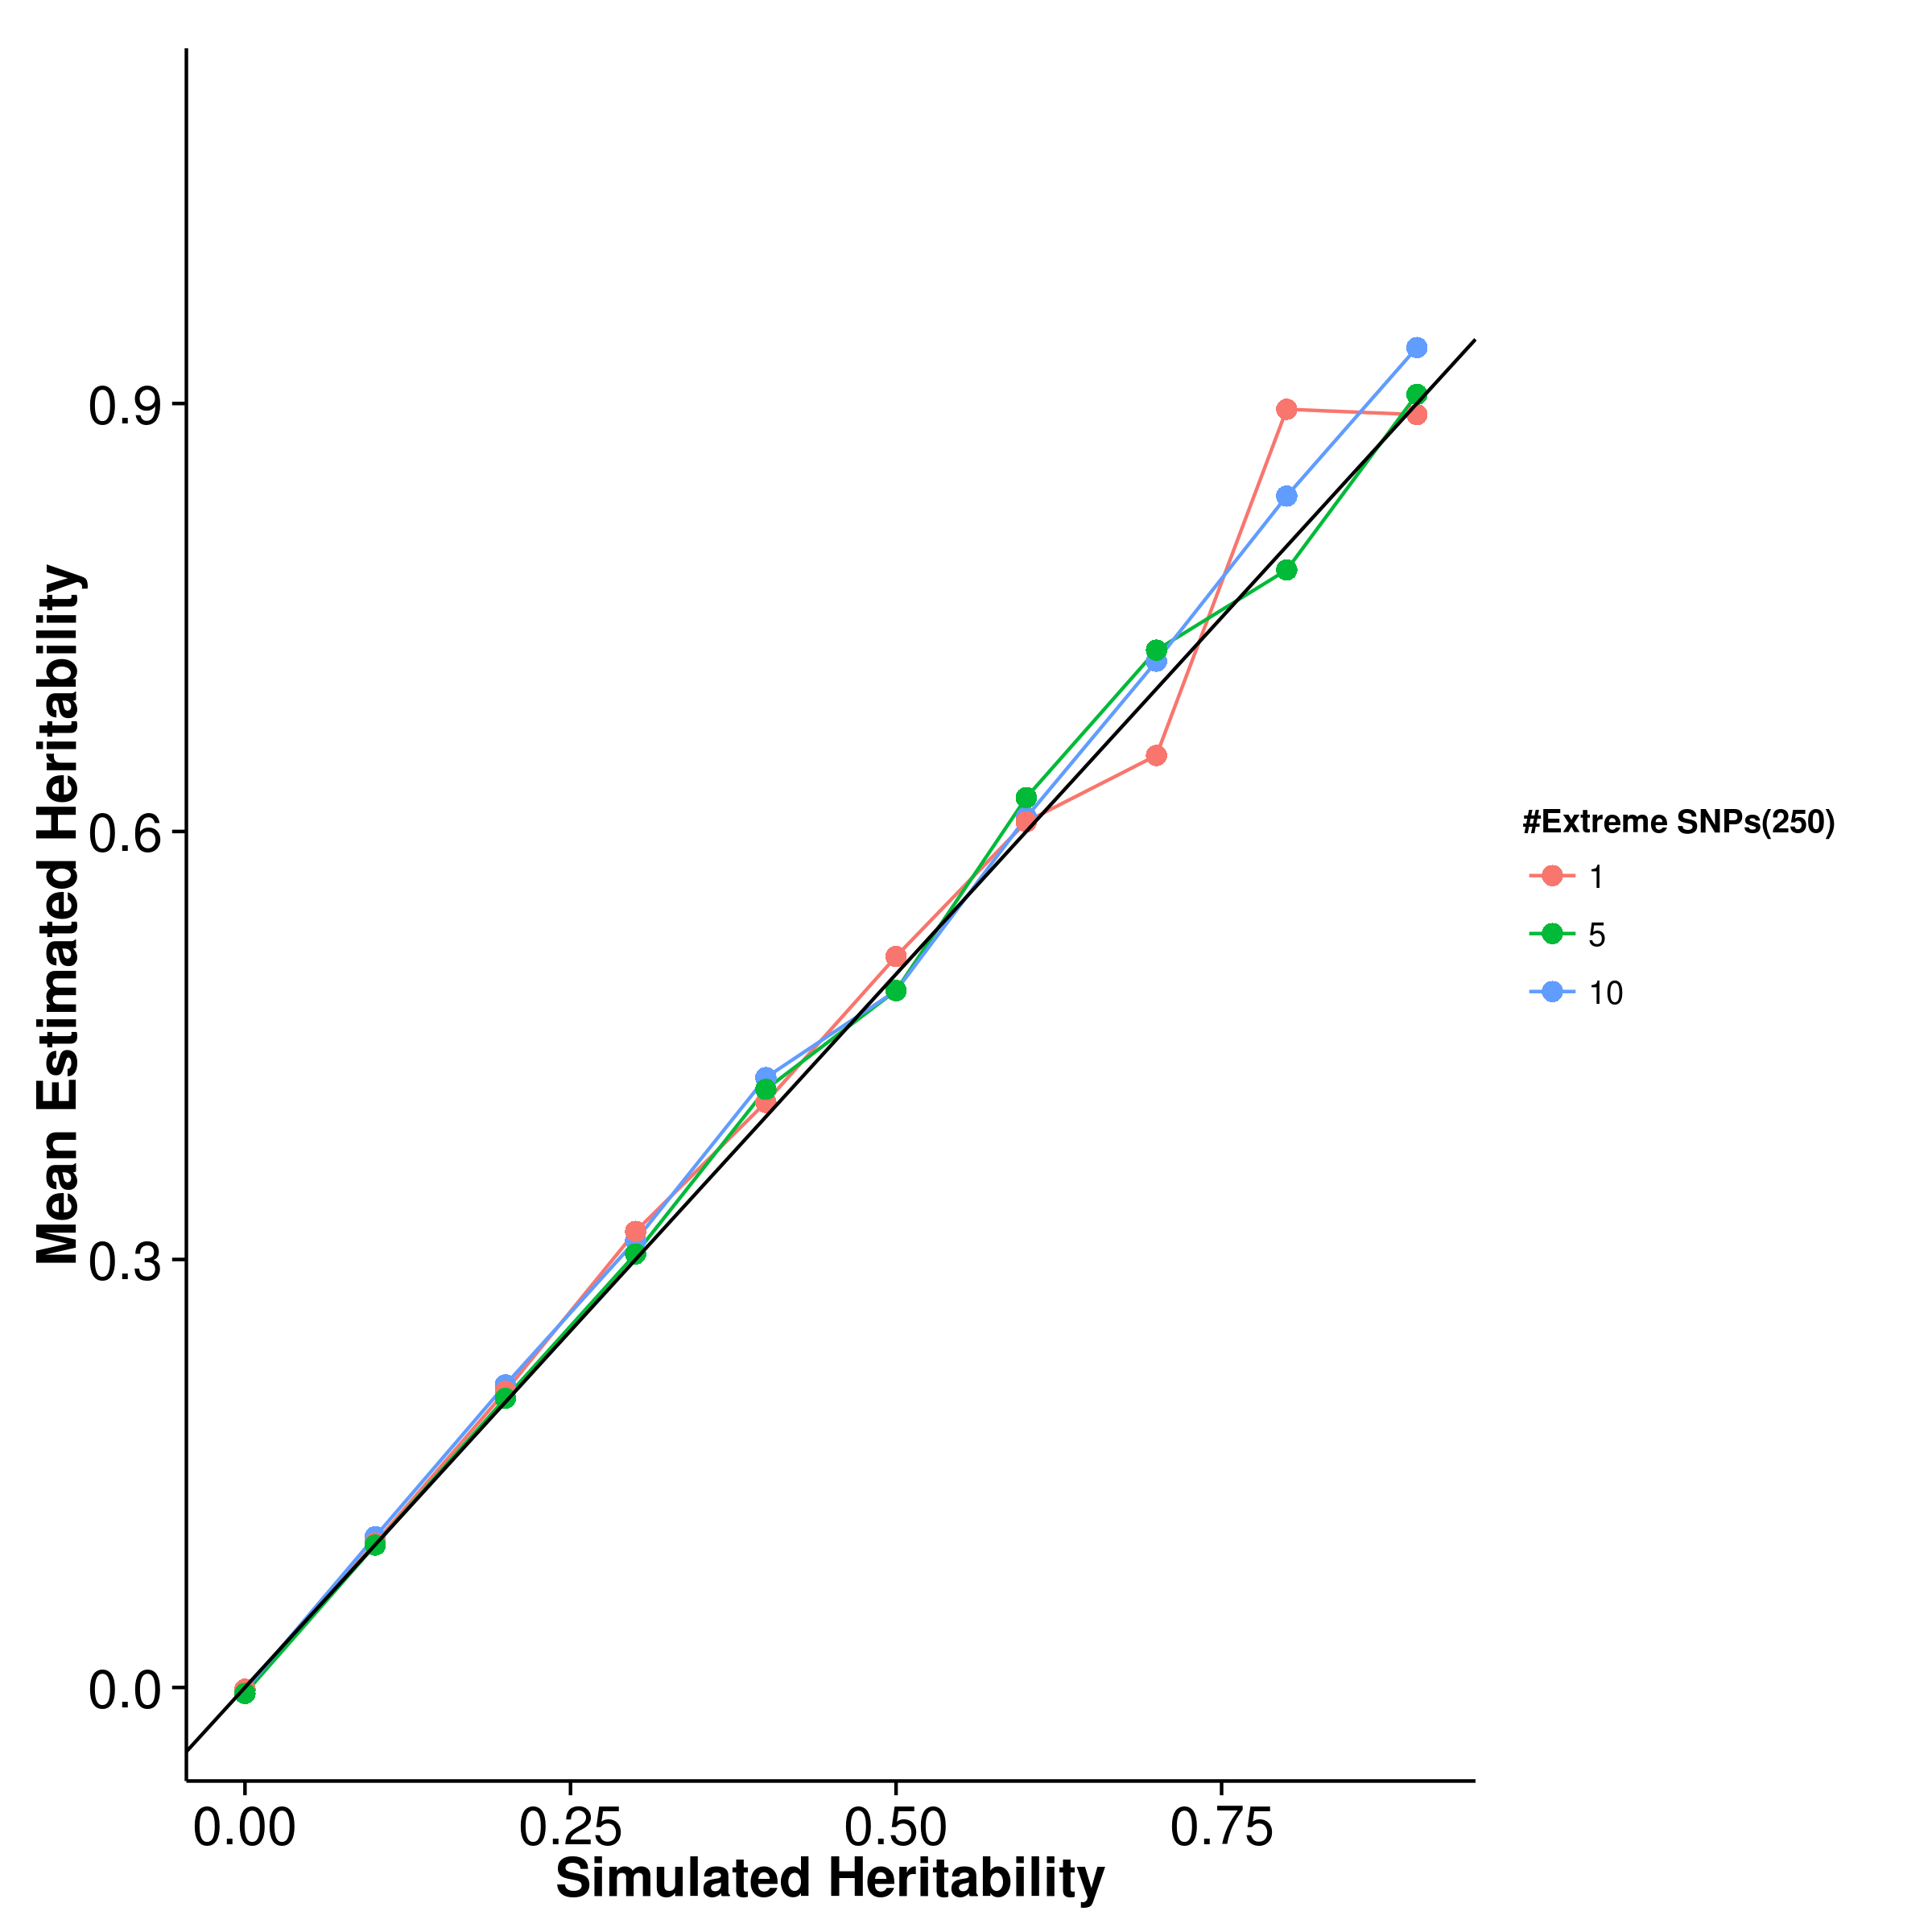
\includegraphics{figure/he_summary/extreme_250c/gcta_QtE_Extreme_mean.png}}
				\label{fig:gctaQtEx250cMean}
			}\\
			\subfloat[LDSC with fix intercept]{
				\scalebox{.4}{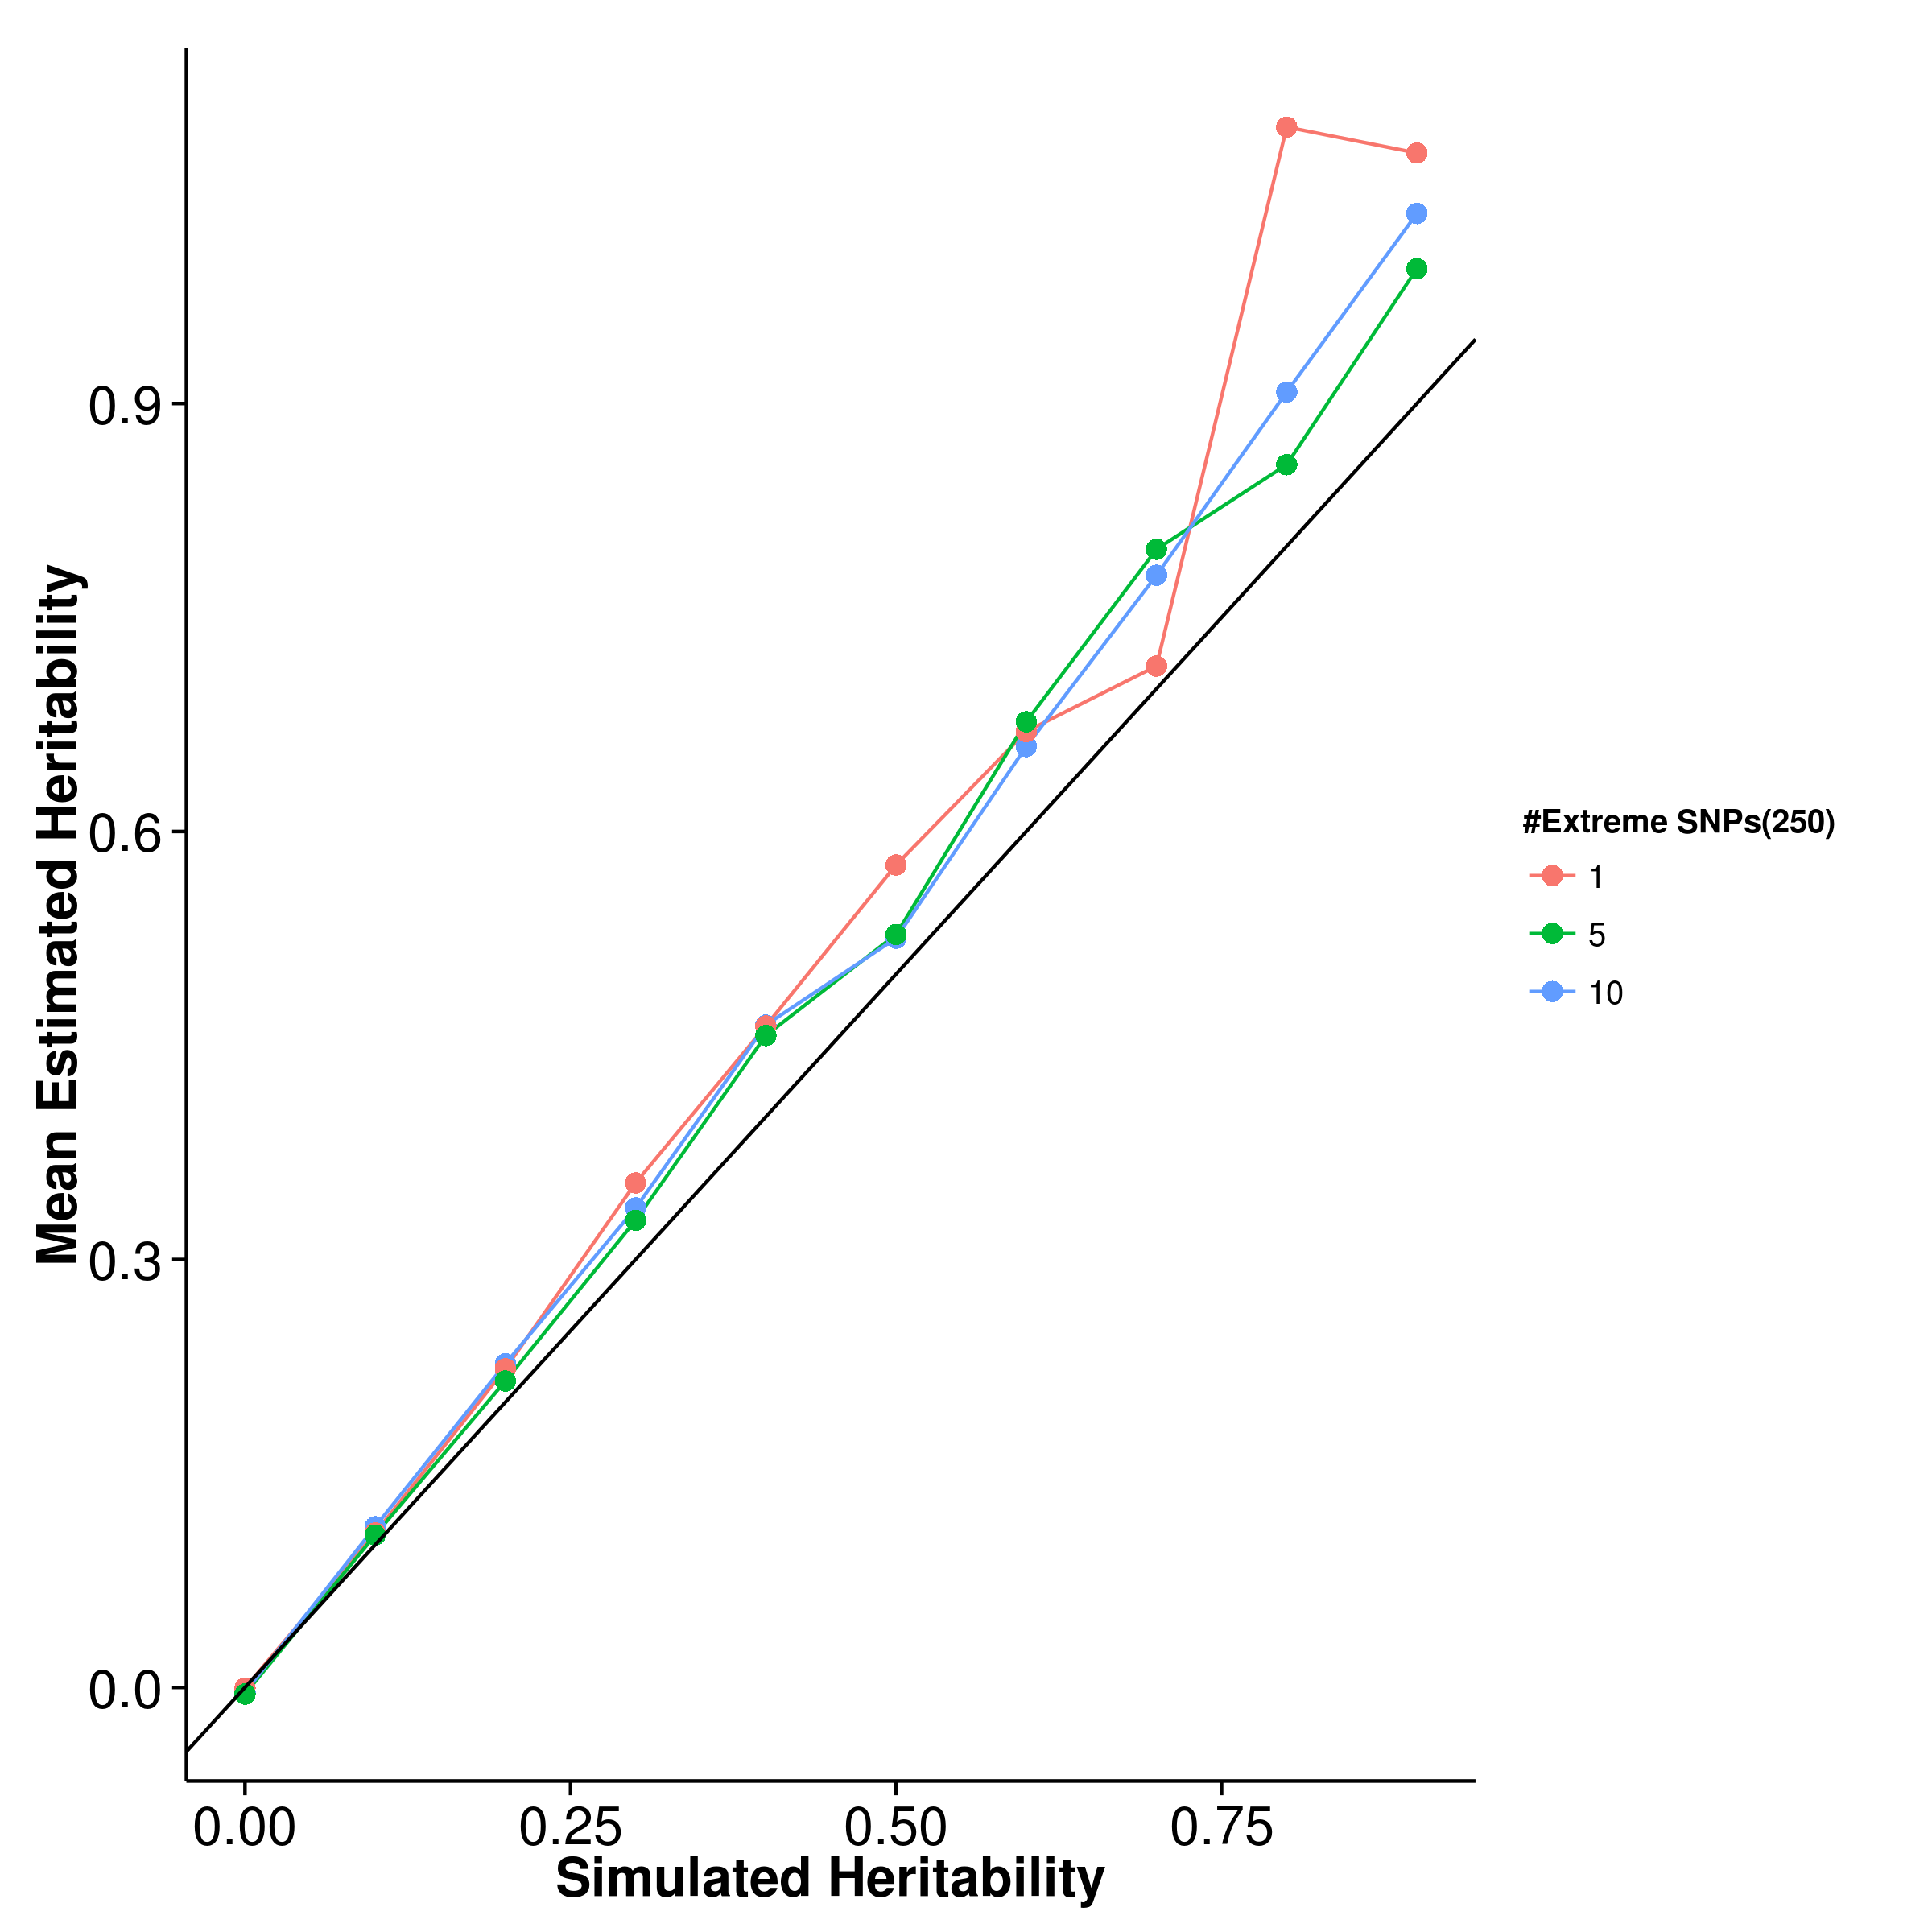
\includegraphics{figure/he_summary/extreme_250c/ldsc_QtE_Extreme_mean.png}}
				\label{fig:ldscQtEx250cMean}
			}
			\subfloat[LDSC with intercept estimation]{
				
				\scalebox{.4}{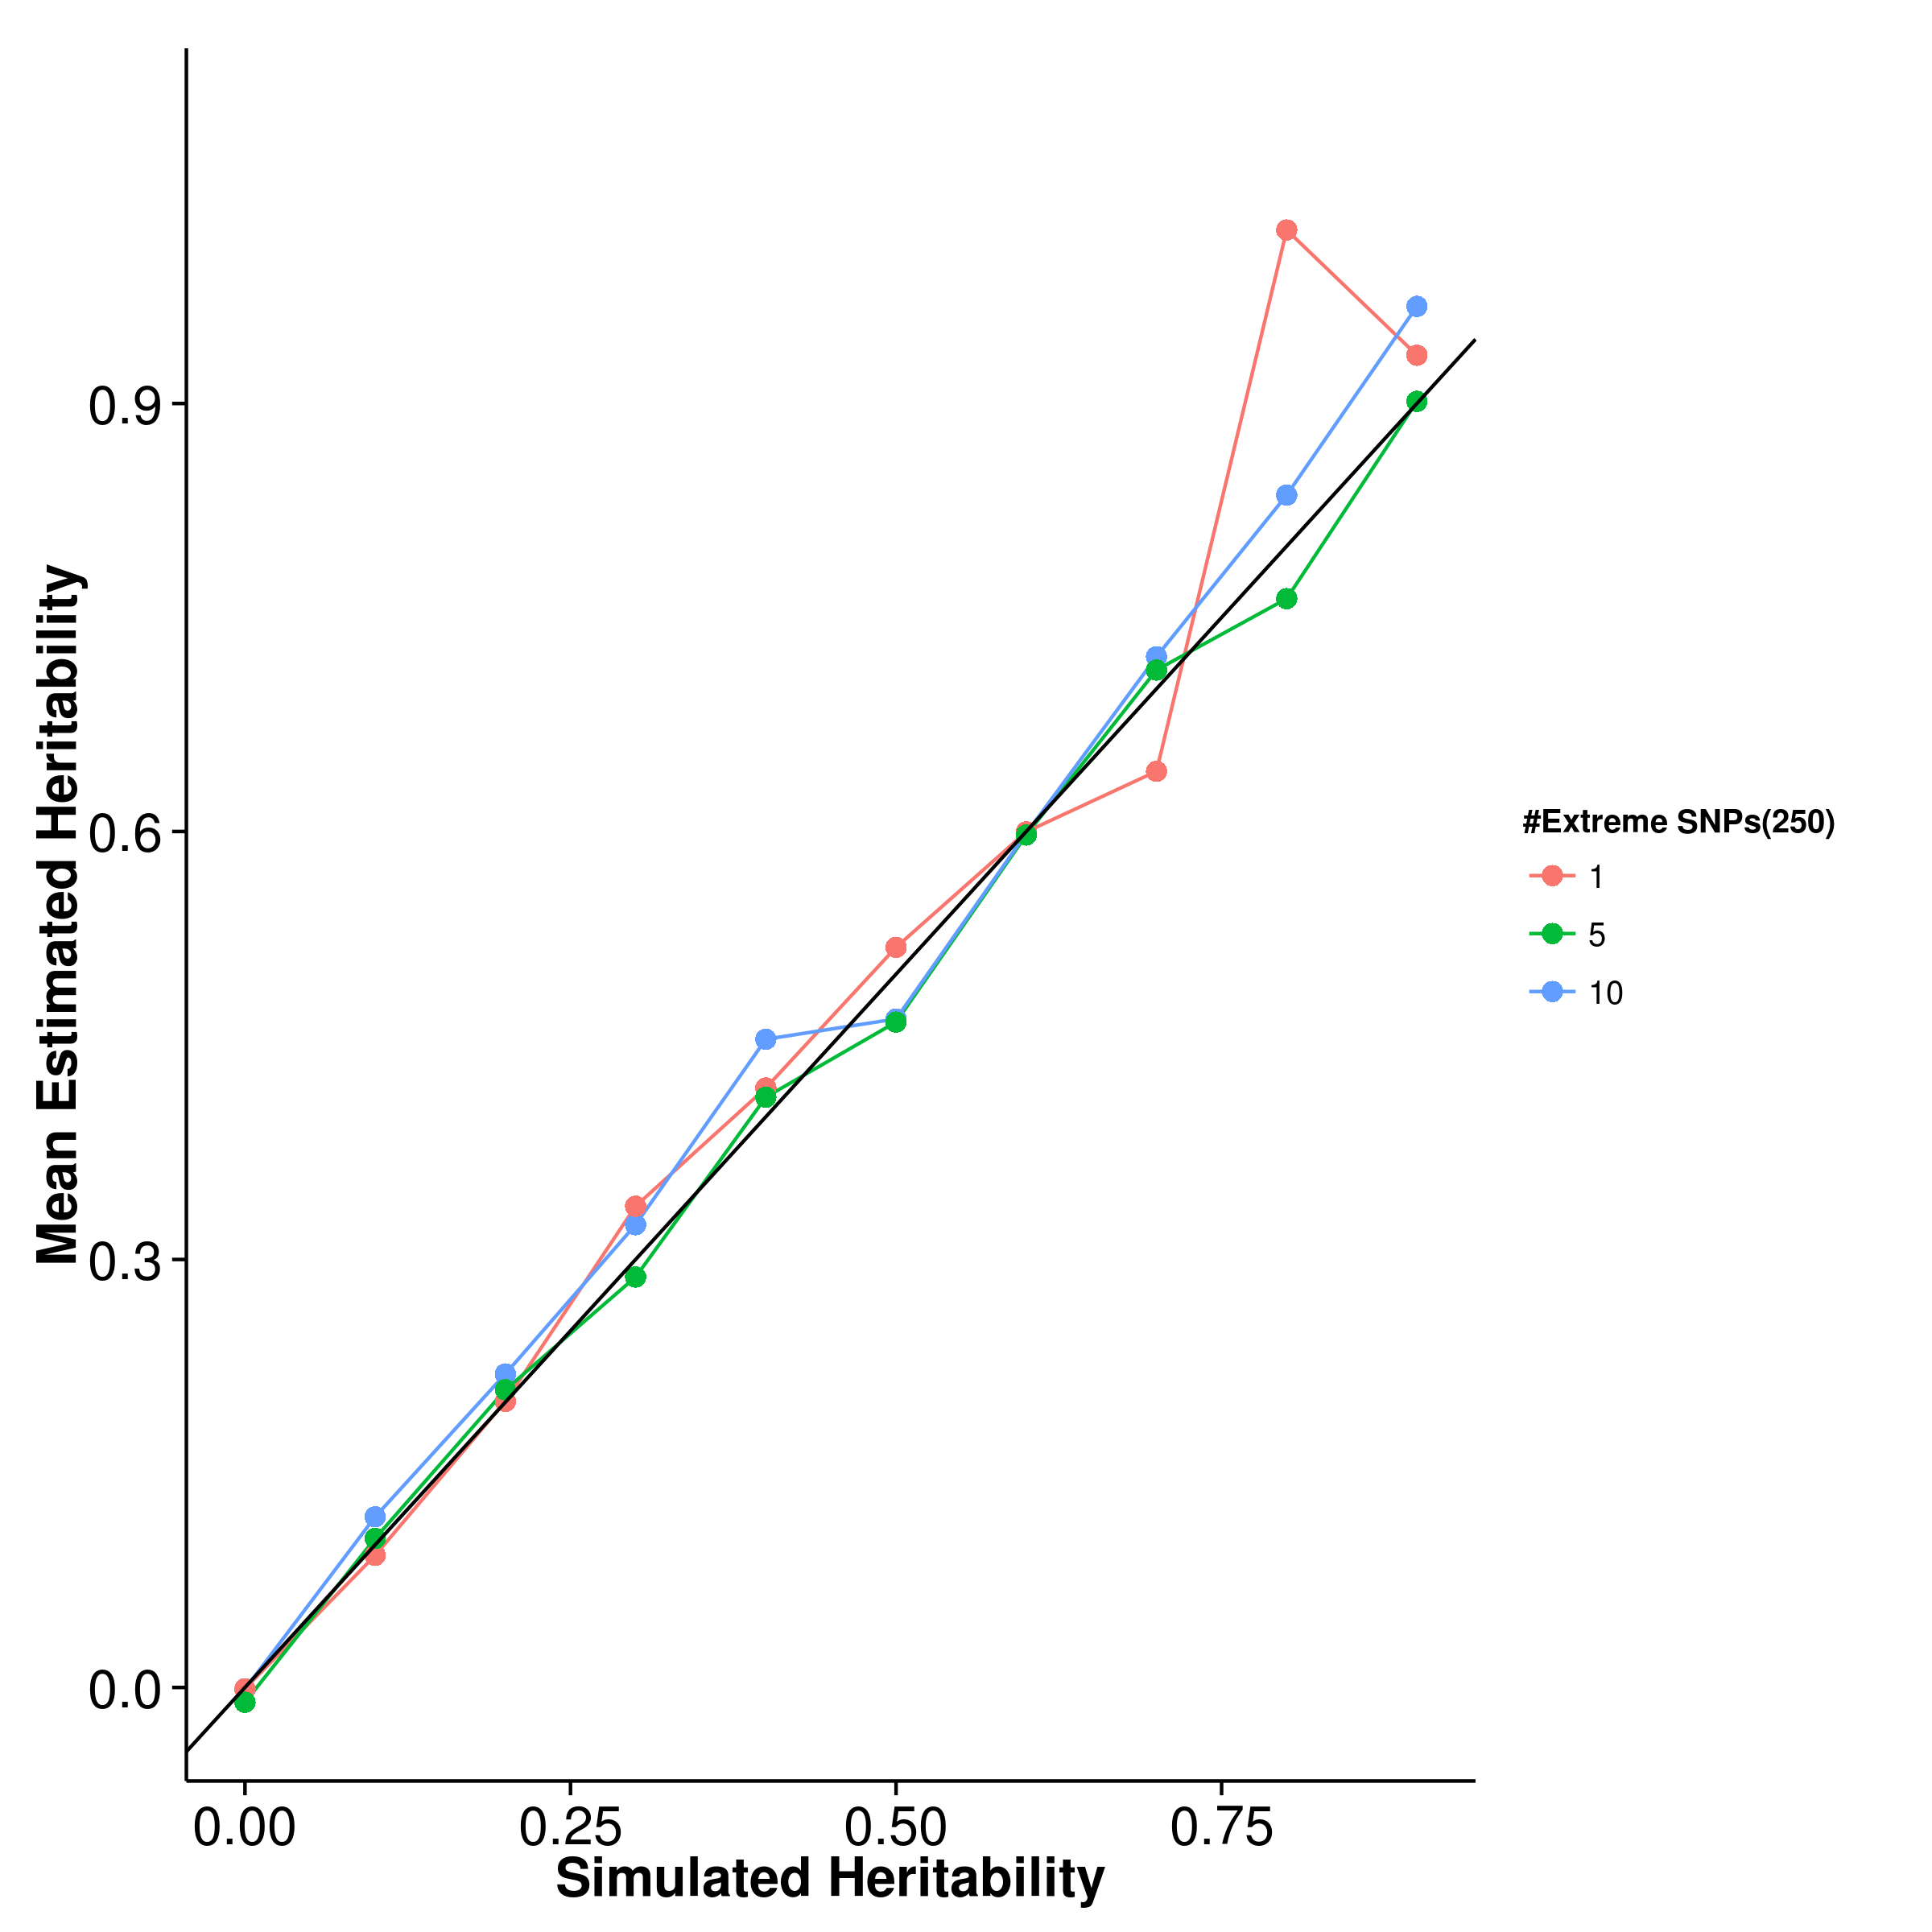
\includegraphics{figure/he_summary/extreme_250c/ldscIn_QtE_Extreme_mean.png}}
				\label{fig:ldscInQtEx250cMean}
			}
			\caption[Quantitative Trait with Extreme Effect Size Simulation Result(250 causal SNPs, Mean)]
			{Mean of results from quantitative trait simulation with extreme effect size simulation.
				250 causal \glspl{SNP} were simulated.
				It was observed that the mean estimation of heritability of all the tools were relatively unaffected by the number of \glspl{SNP} representing a large portion of effect, similar to what observed when 100 causal \glspl{SNP} were simulated.
				However, there seems to be an upward bias when \gls{ldsc} was performed with fixed intercept.
			} 
			\label{fig:QtEx250cMean}
		\end{figure}
		
		\begin{figure}
			\centering
			\subfloat[SHREK]{
				\scalebox{.4}{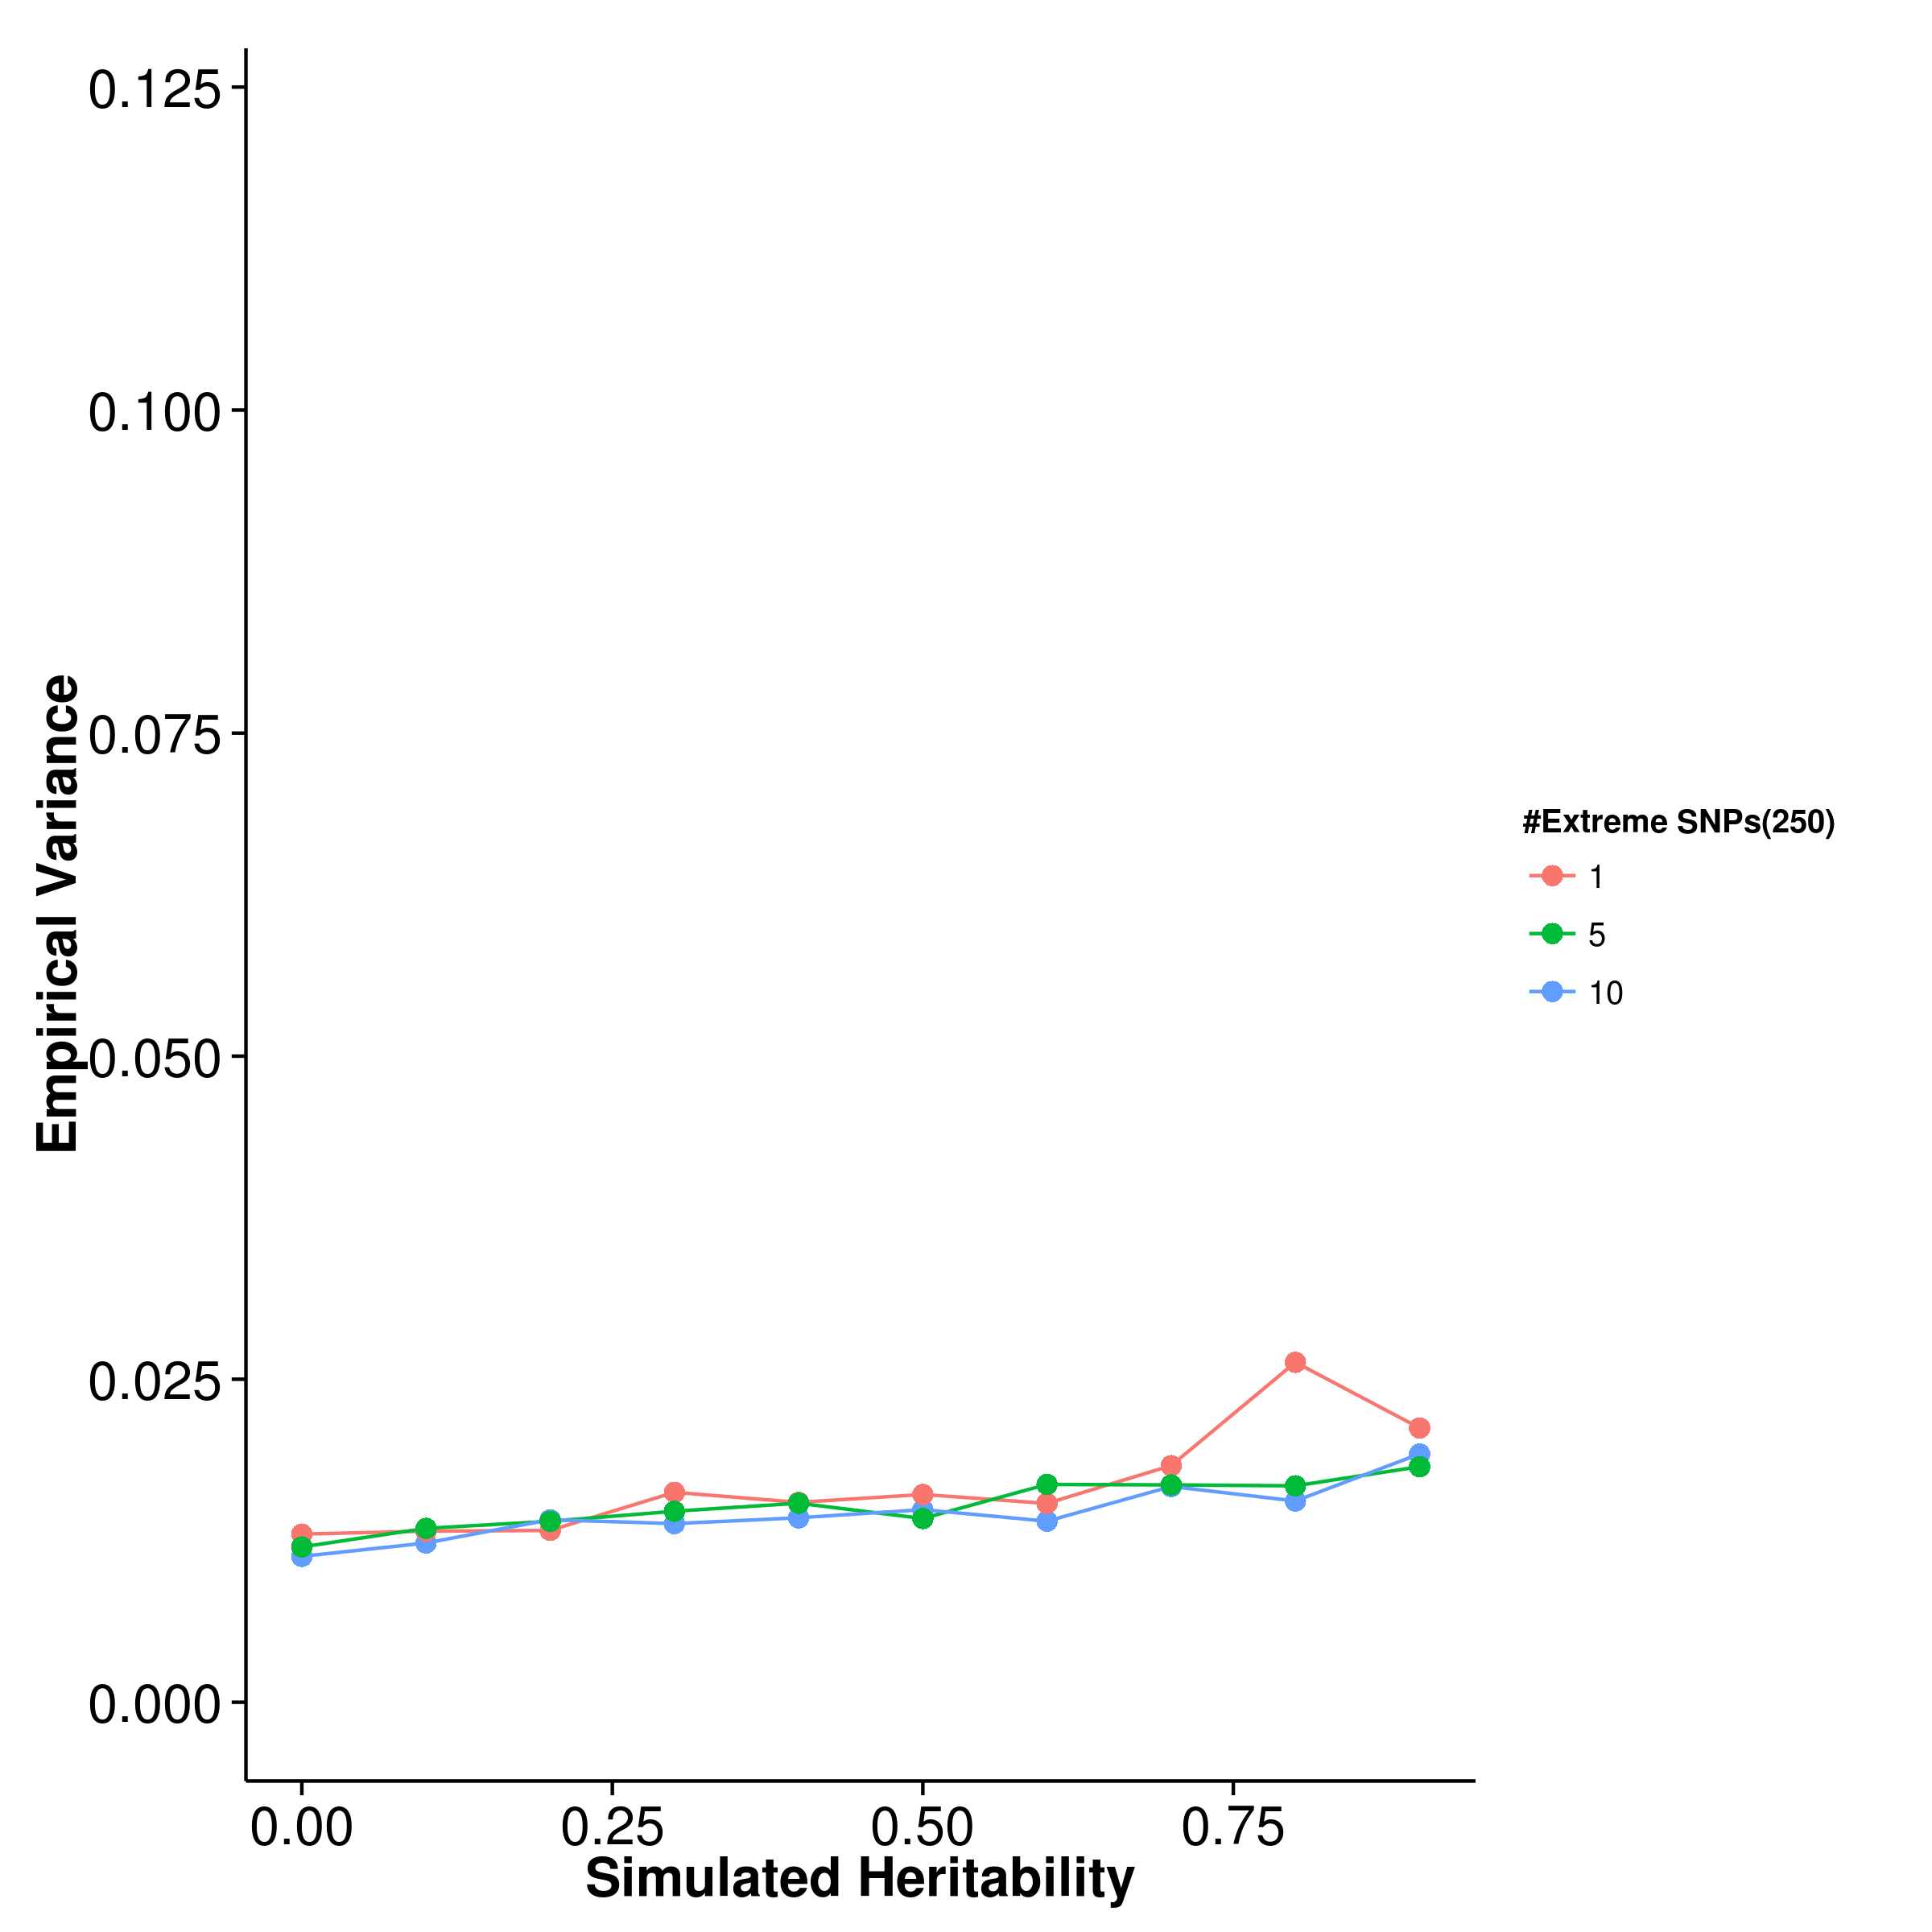
\includegraphics{figure/he_summary/extreme_250c/shrek_QtE_Extreme_sd.png}}
				\label{fig:shrekQtEx250cVar}
			}
			\subfloat[GCTA]{
				\scalebox{.4}{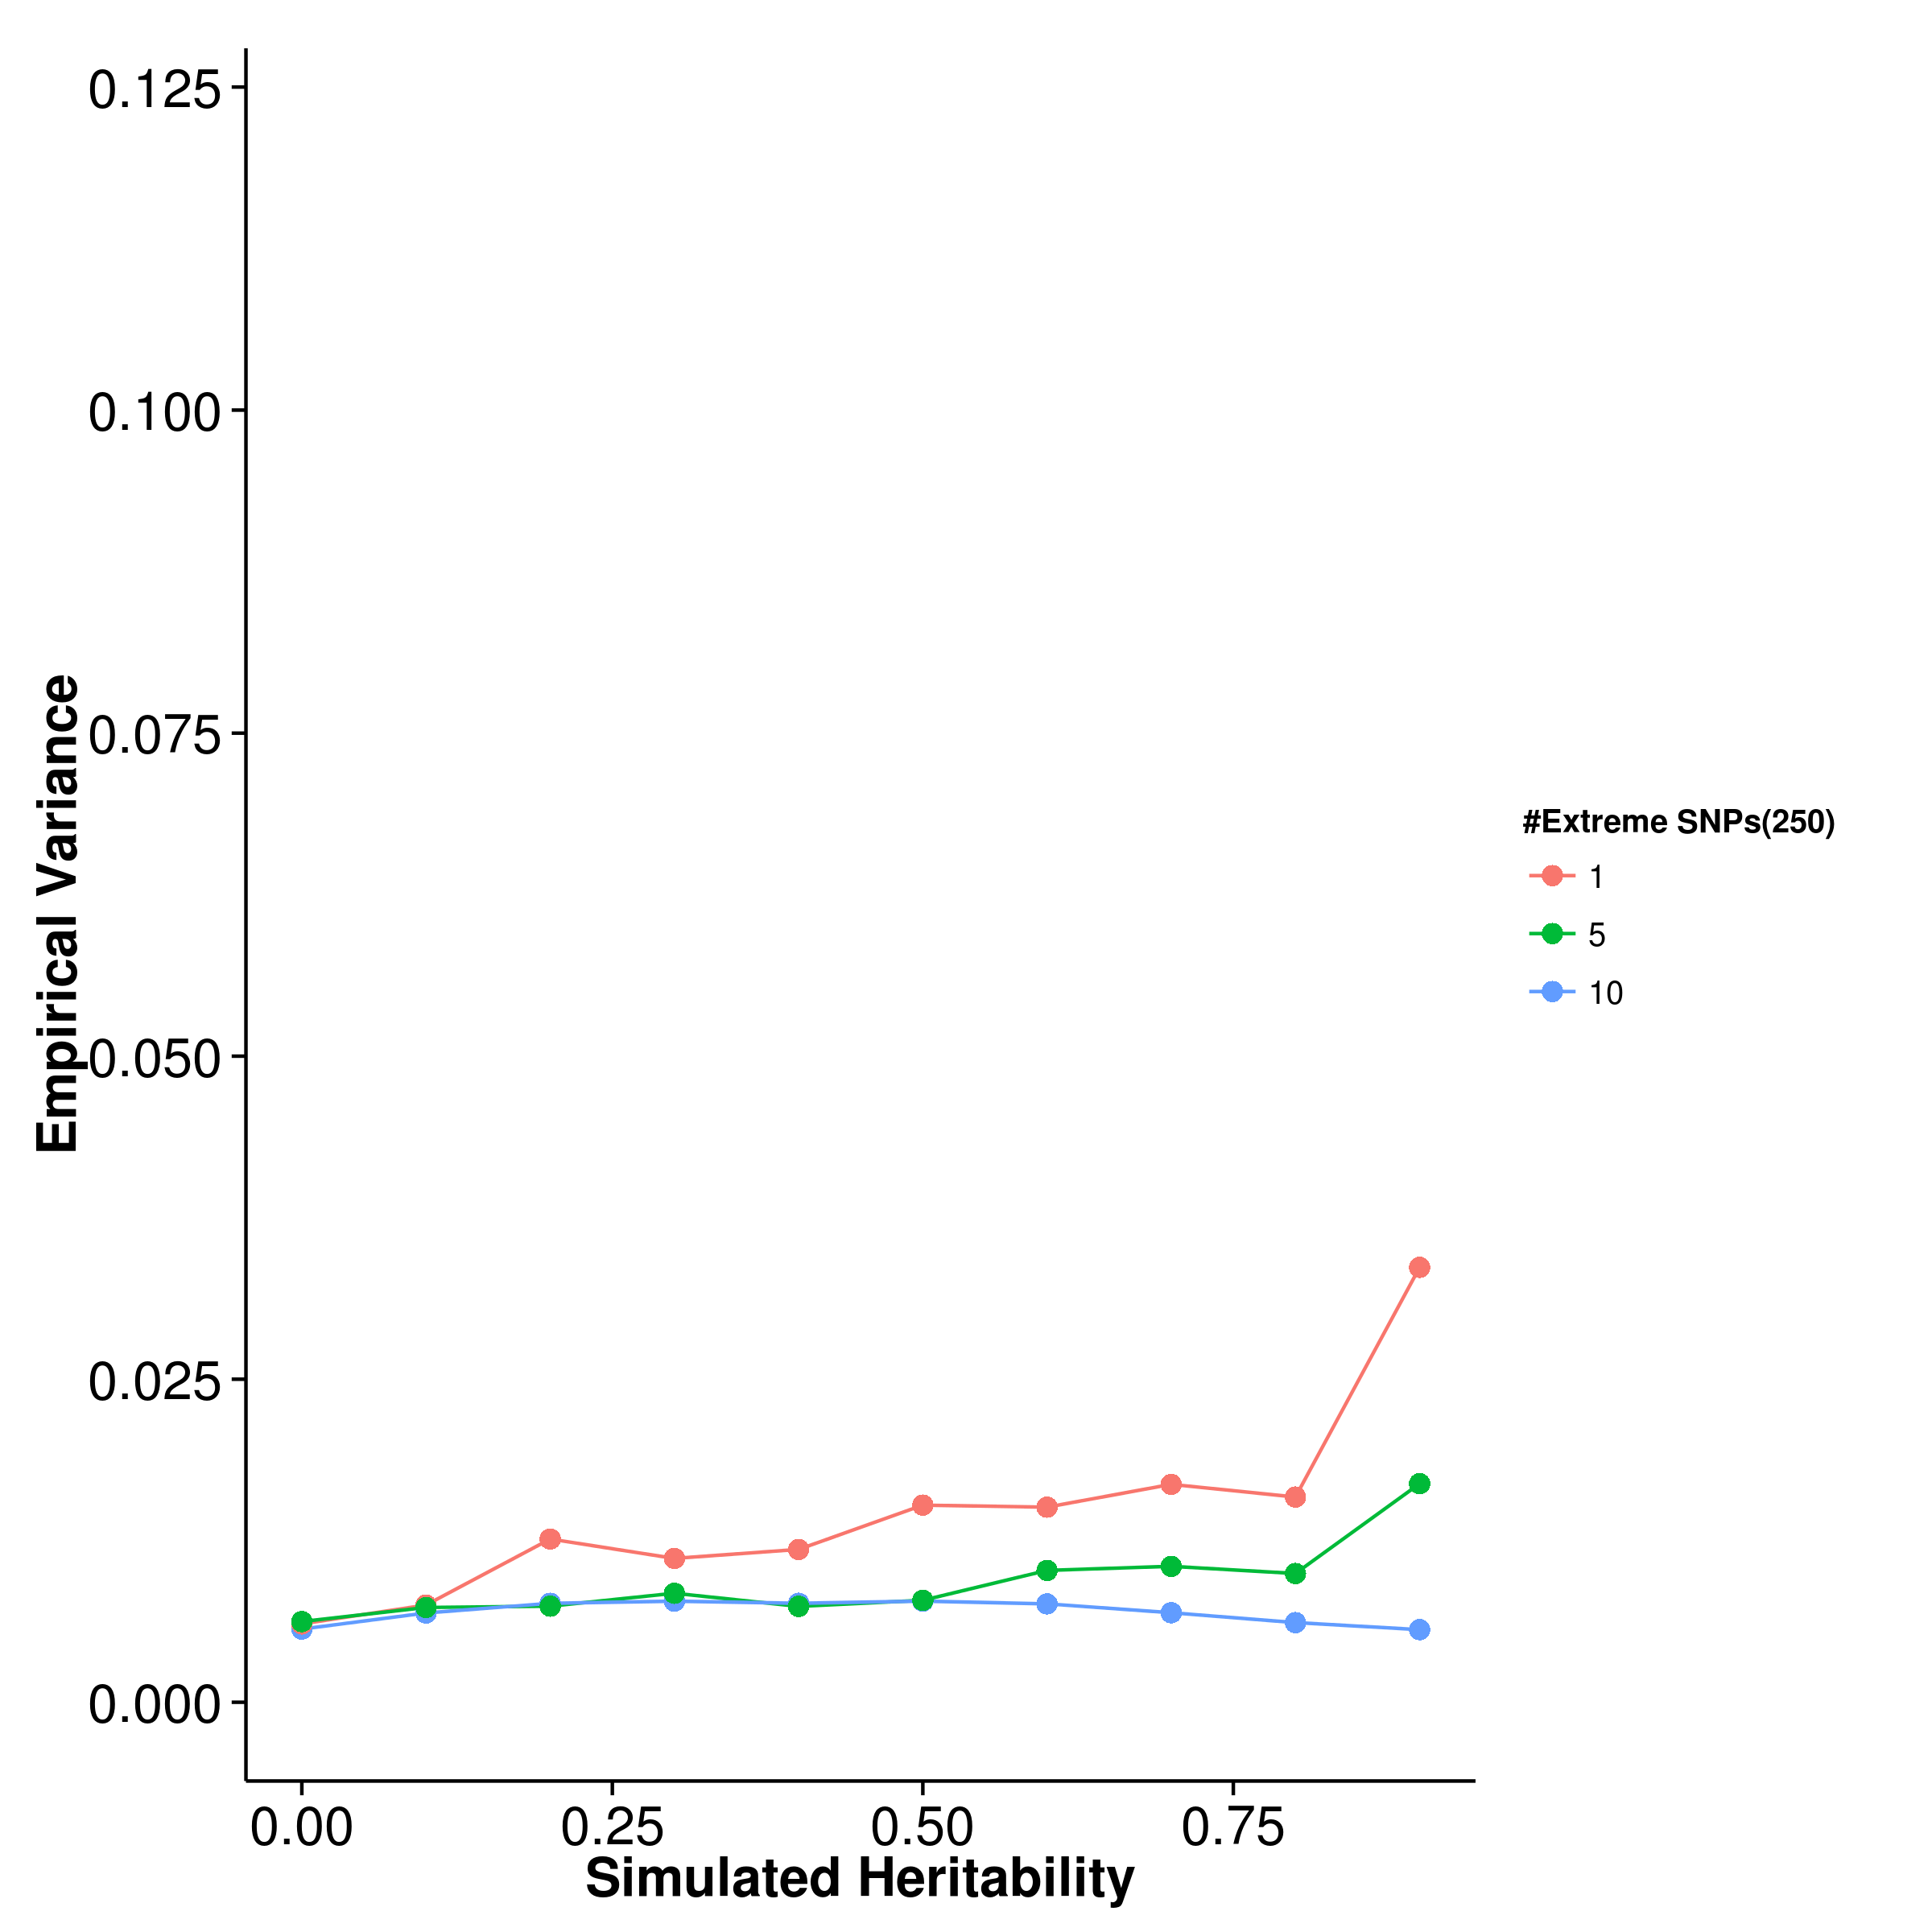
\includegraphics{figure/he_summary/extreme_250c/gcta_QtE_Extreme_sd.png}}
				\label{fig:gctaQtEx250cVar}
			}\\
			\subfloat[LDSC with fix intercept]{
				\scalebox{.4}{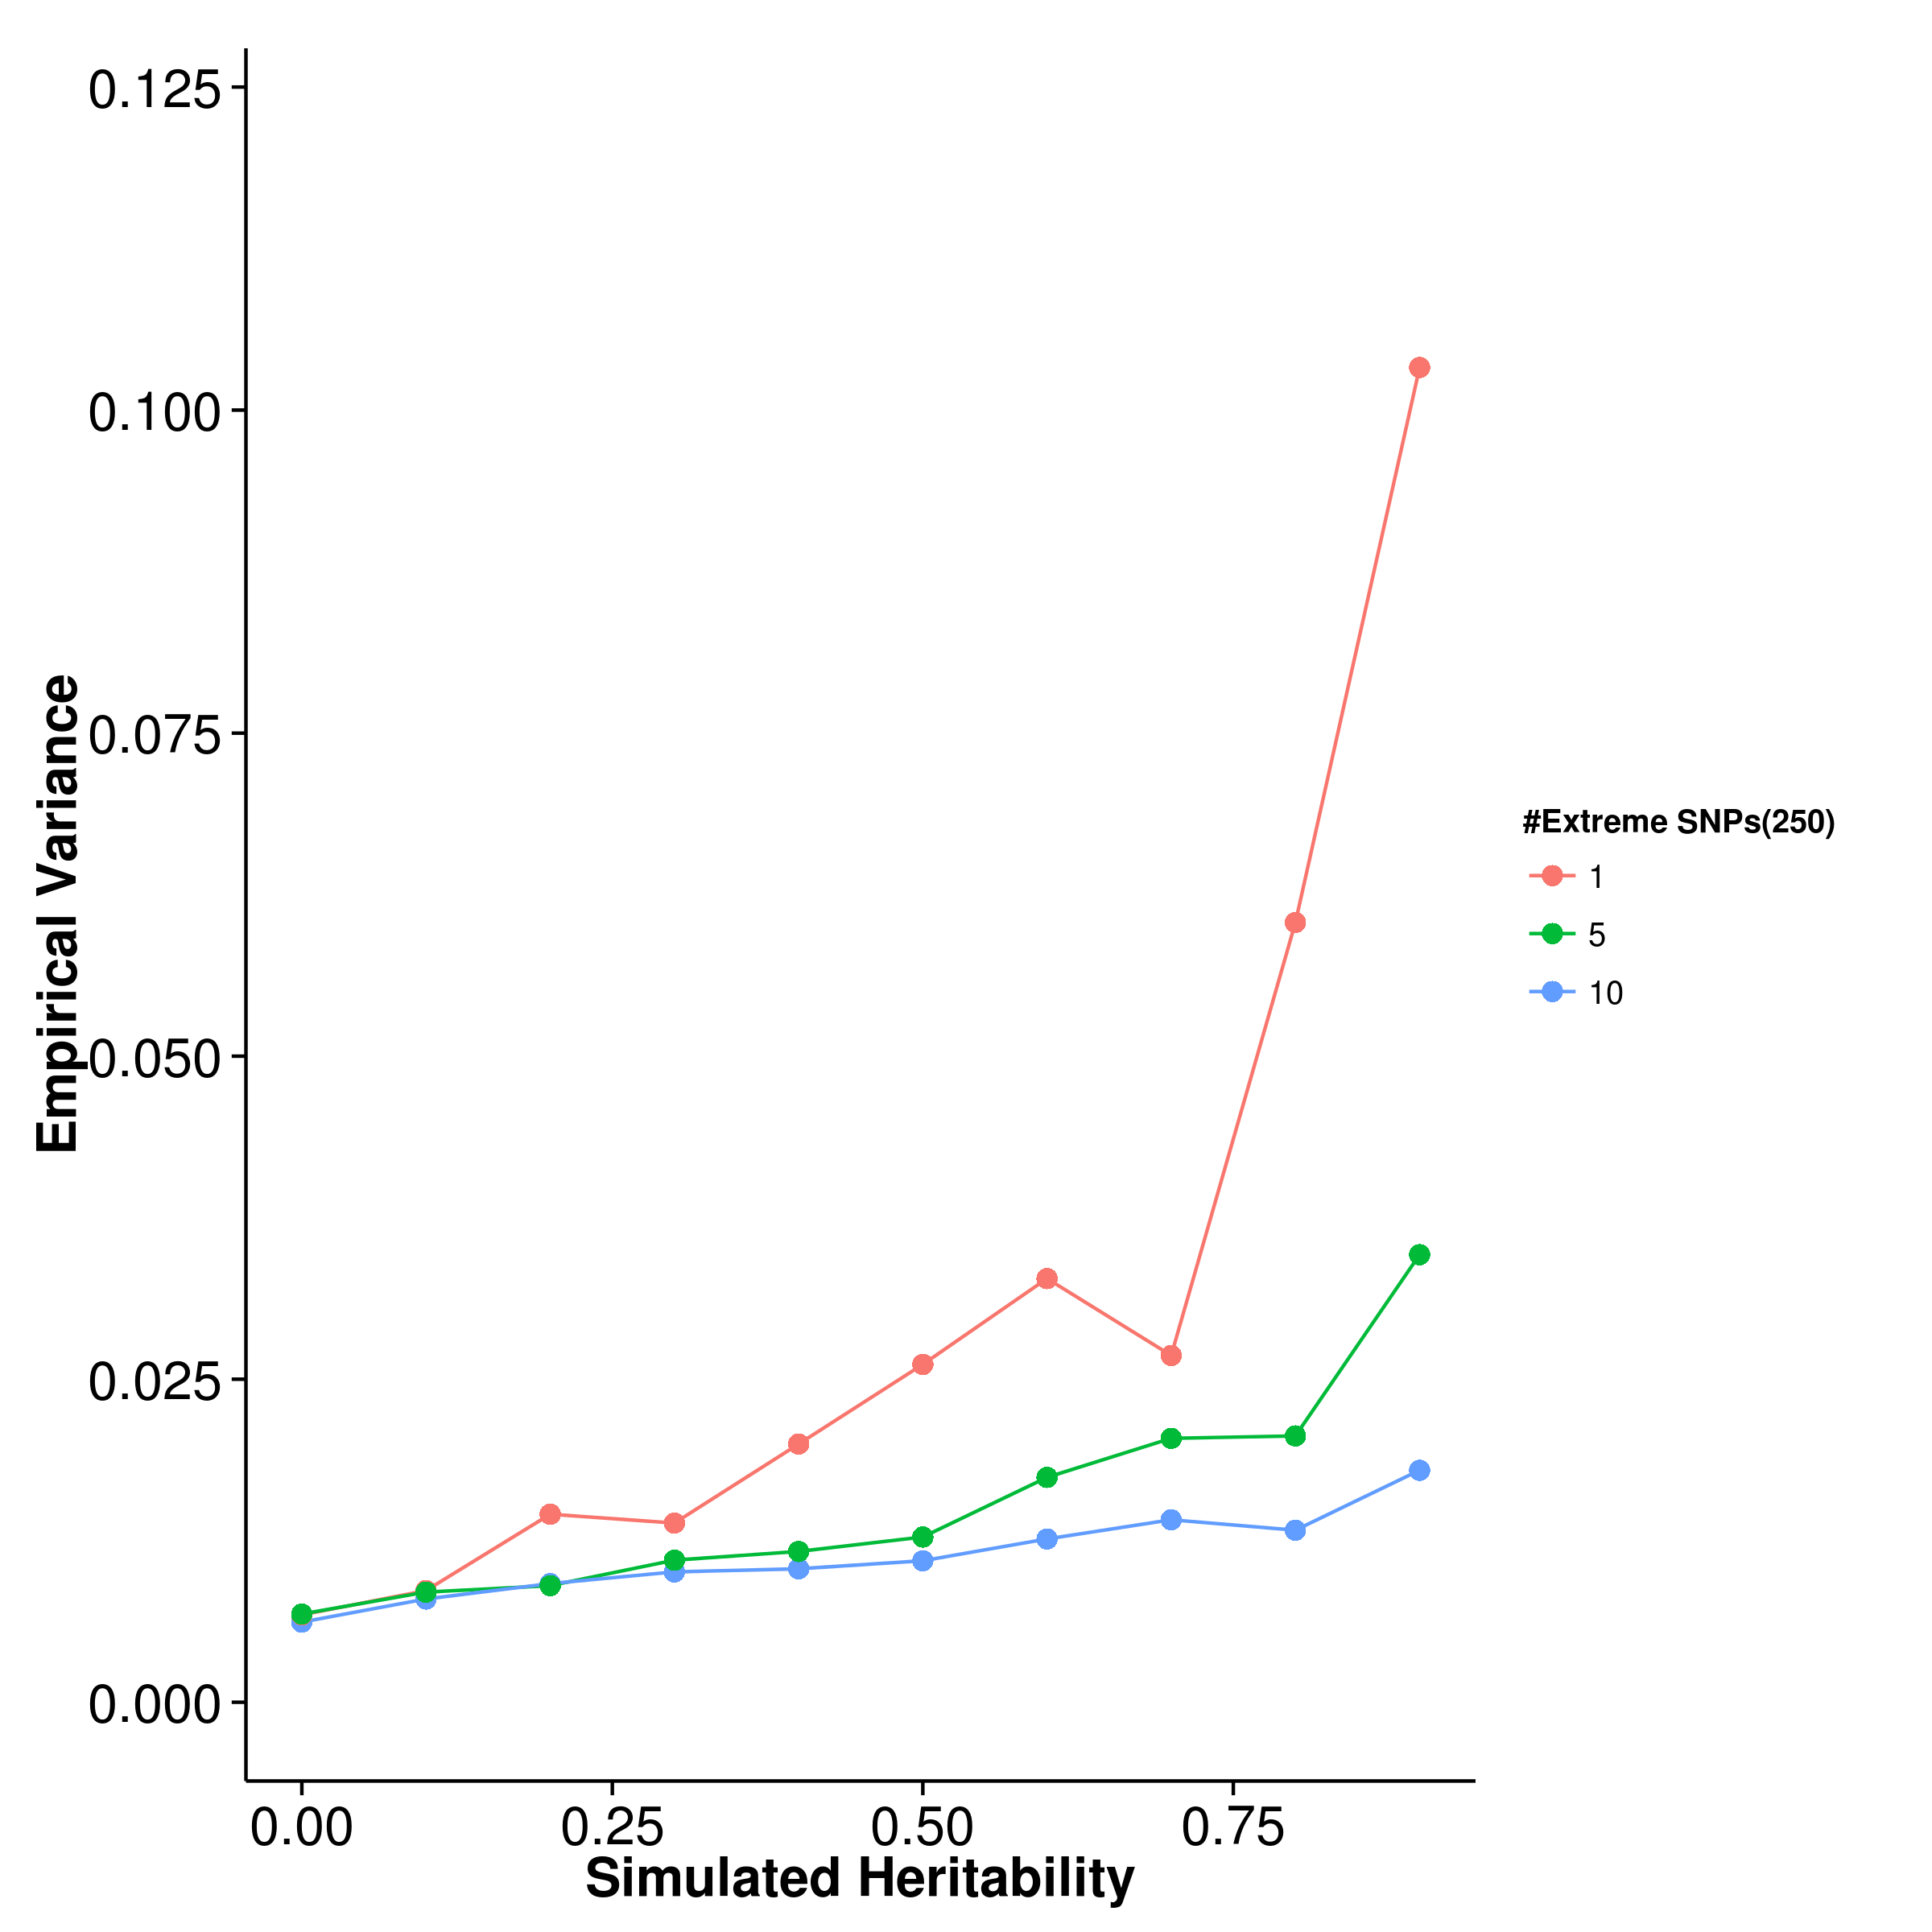
\includegraphics{figure/he_summary/extreme_250c/ldsc_QtE_Extreme_sd.png}}
				\label{fig:ldscQtEx250cVar}
			}
			\subfloat[LDSC with intercept estimation]{
				
				\scalebox{.4}{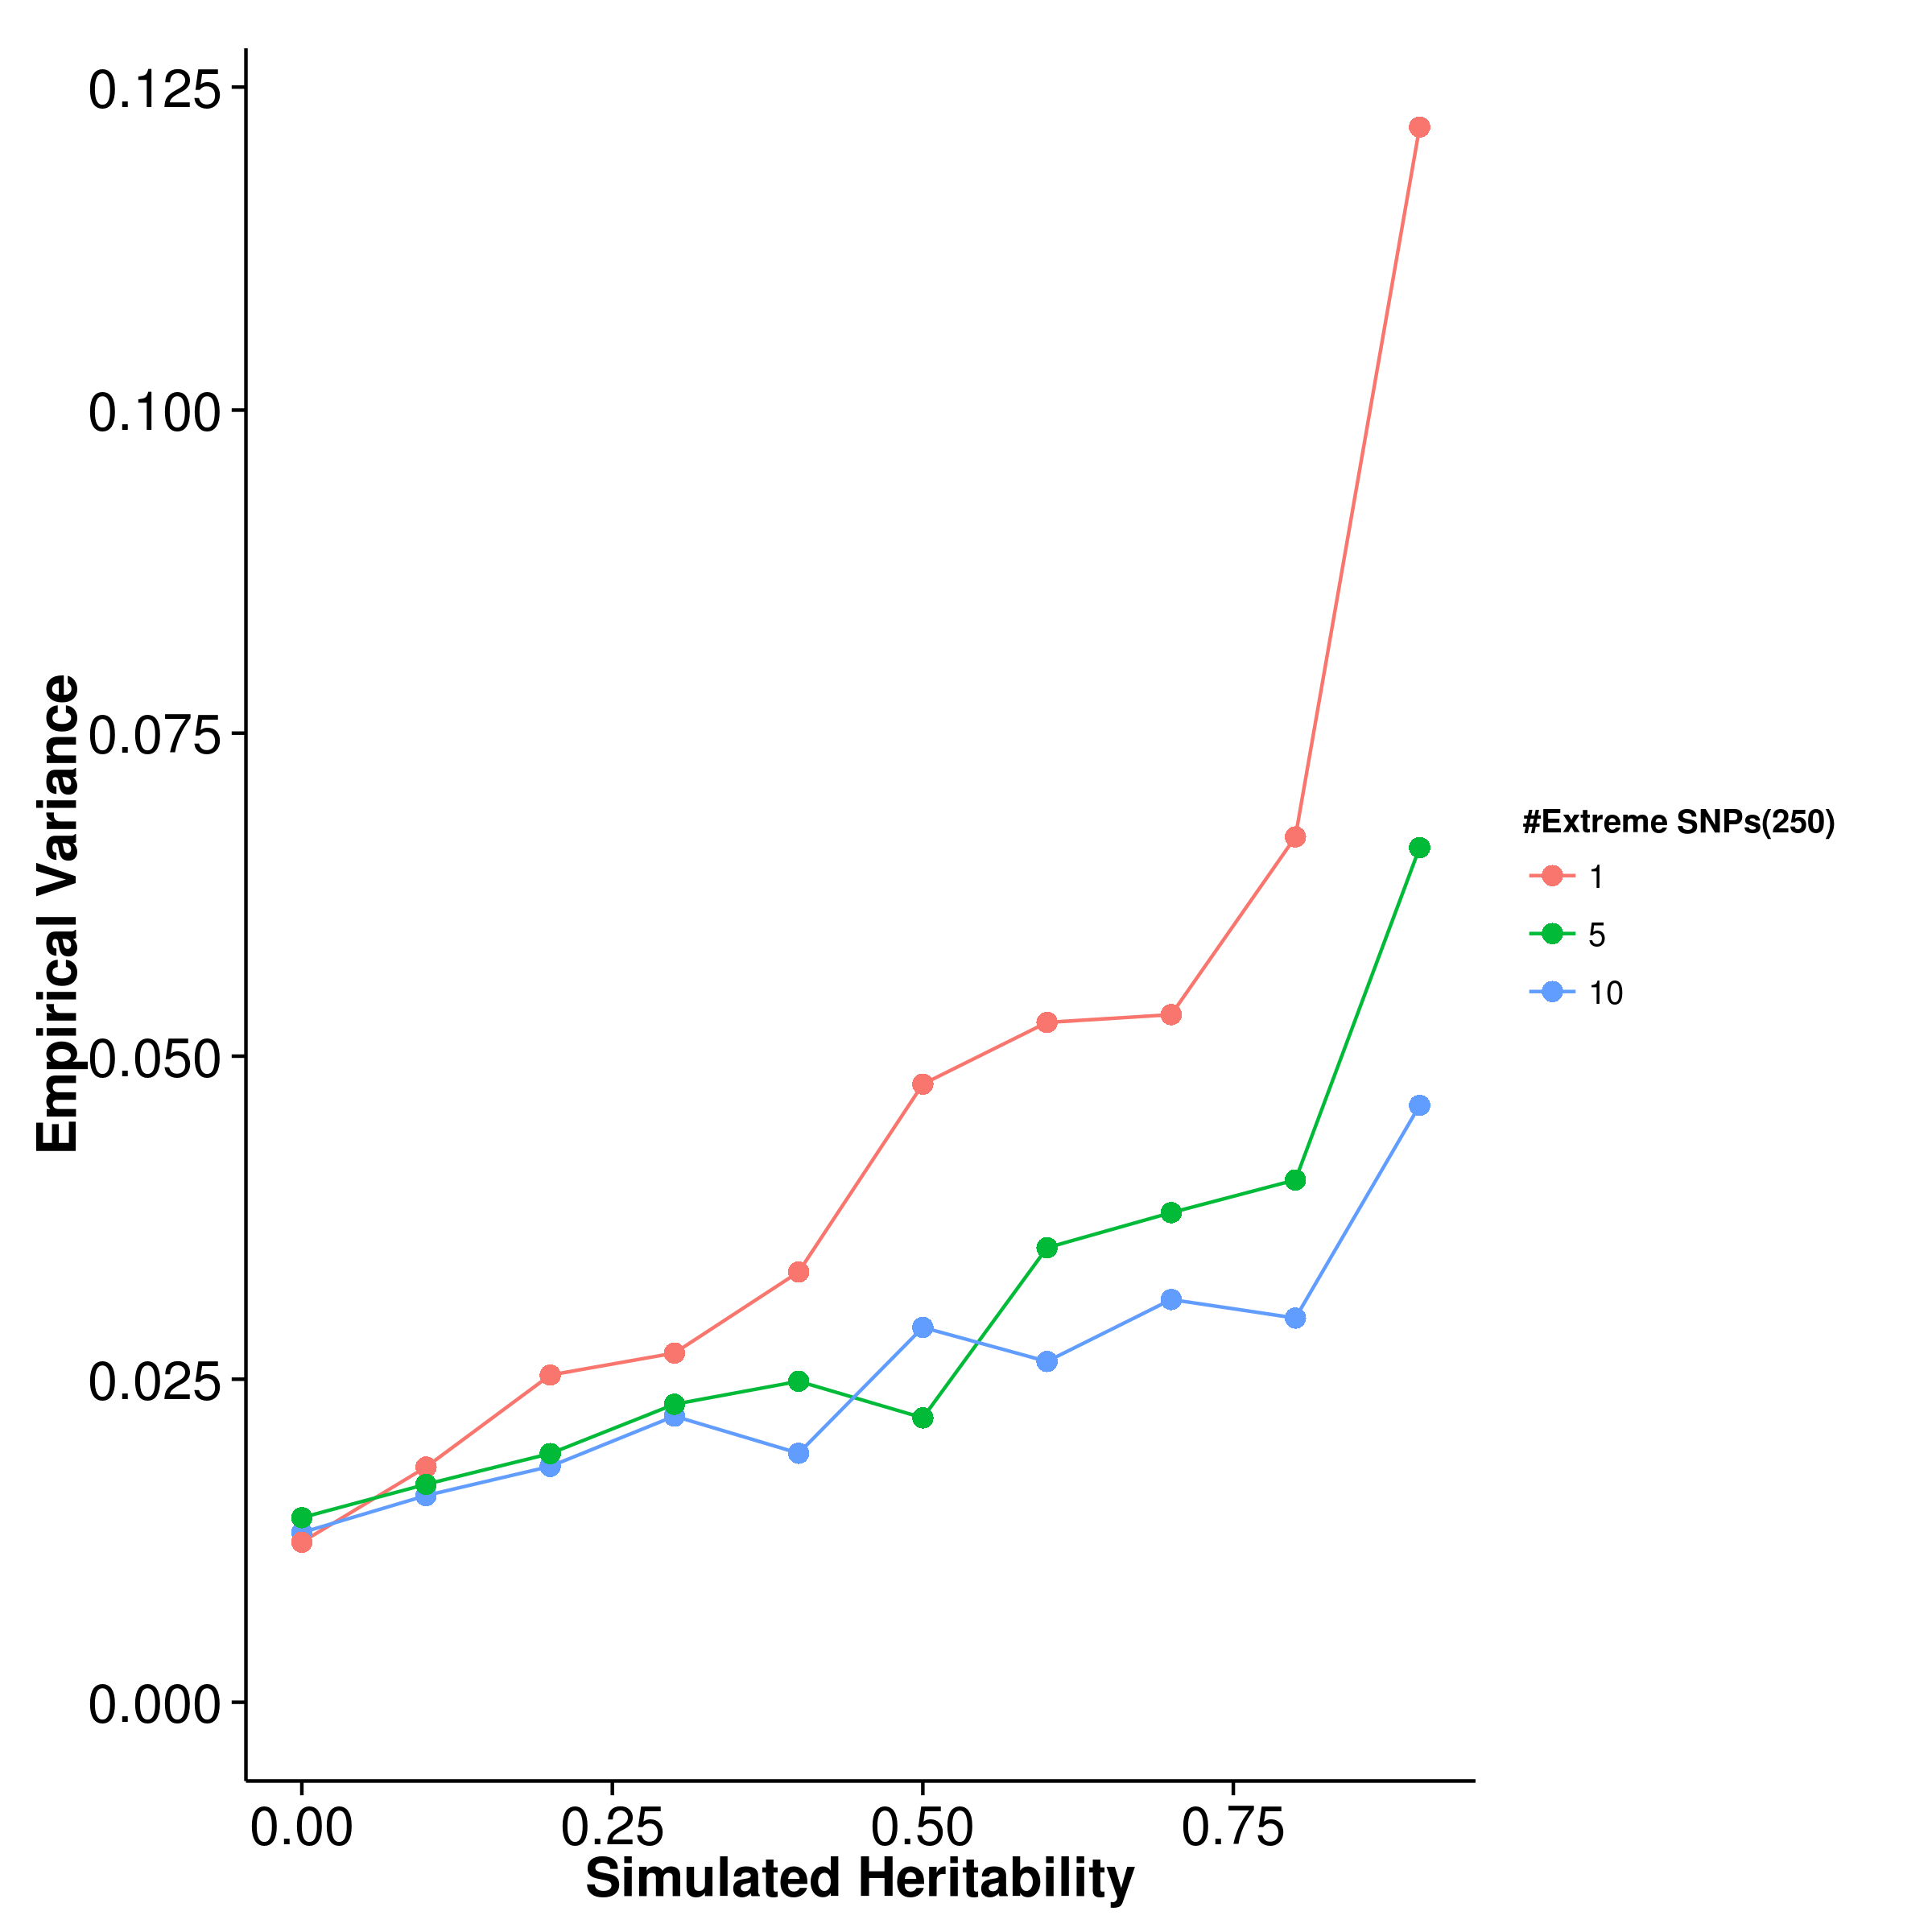
\includegraphics{figure/he_summary/extreme_250c/ldscIn_QtE_Extreme_sd.png}}
				\label{fig:ldscInQtEx250cVar}
			}
			\caption[Quantitative Trait with Extreme Effect Size Simulation Result(250 causal SNPs, Variance)]
			{Variance of results from quantitative trait simulation with extreme effect size simulation.
				250 causal \glspl{SNP} were simulated.
				Compared to the case where 100 causal \glspl{SNP} were simulated, most tools, except \gls{shrek} seems to be more sensitive to the number of \gls{SNP}(s) explaining large portion of effect, where a smaller number can lead to a higher variance.
			} 
			\label{fig:QtEx250cVar}
		\end{figure}
		
		\begin{figure}
			\centering
			\subfloat[SHREK]{
				\scalebox{.4}{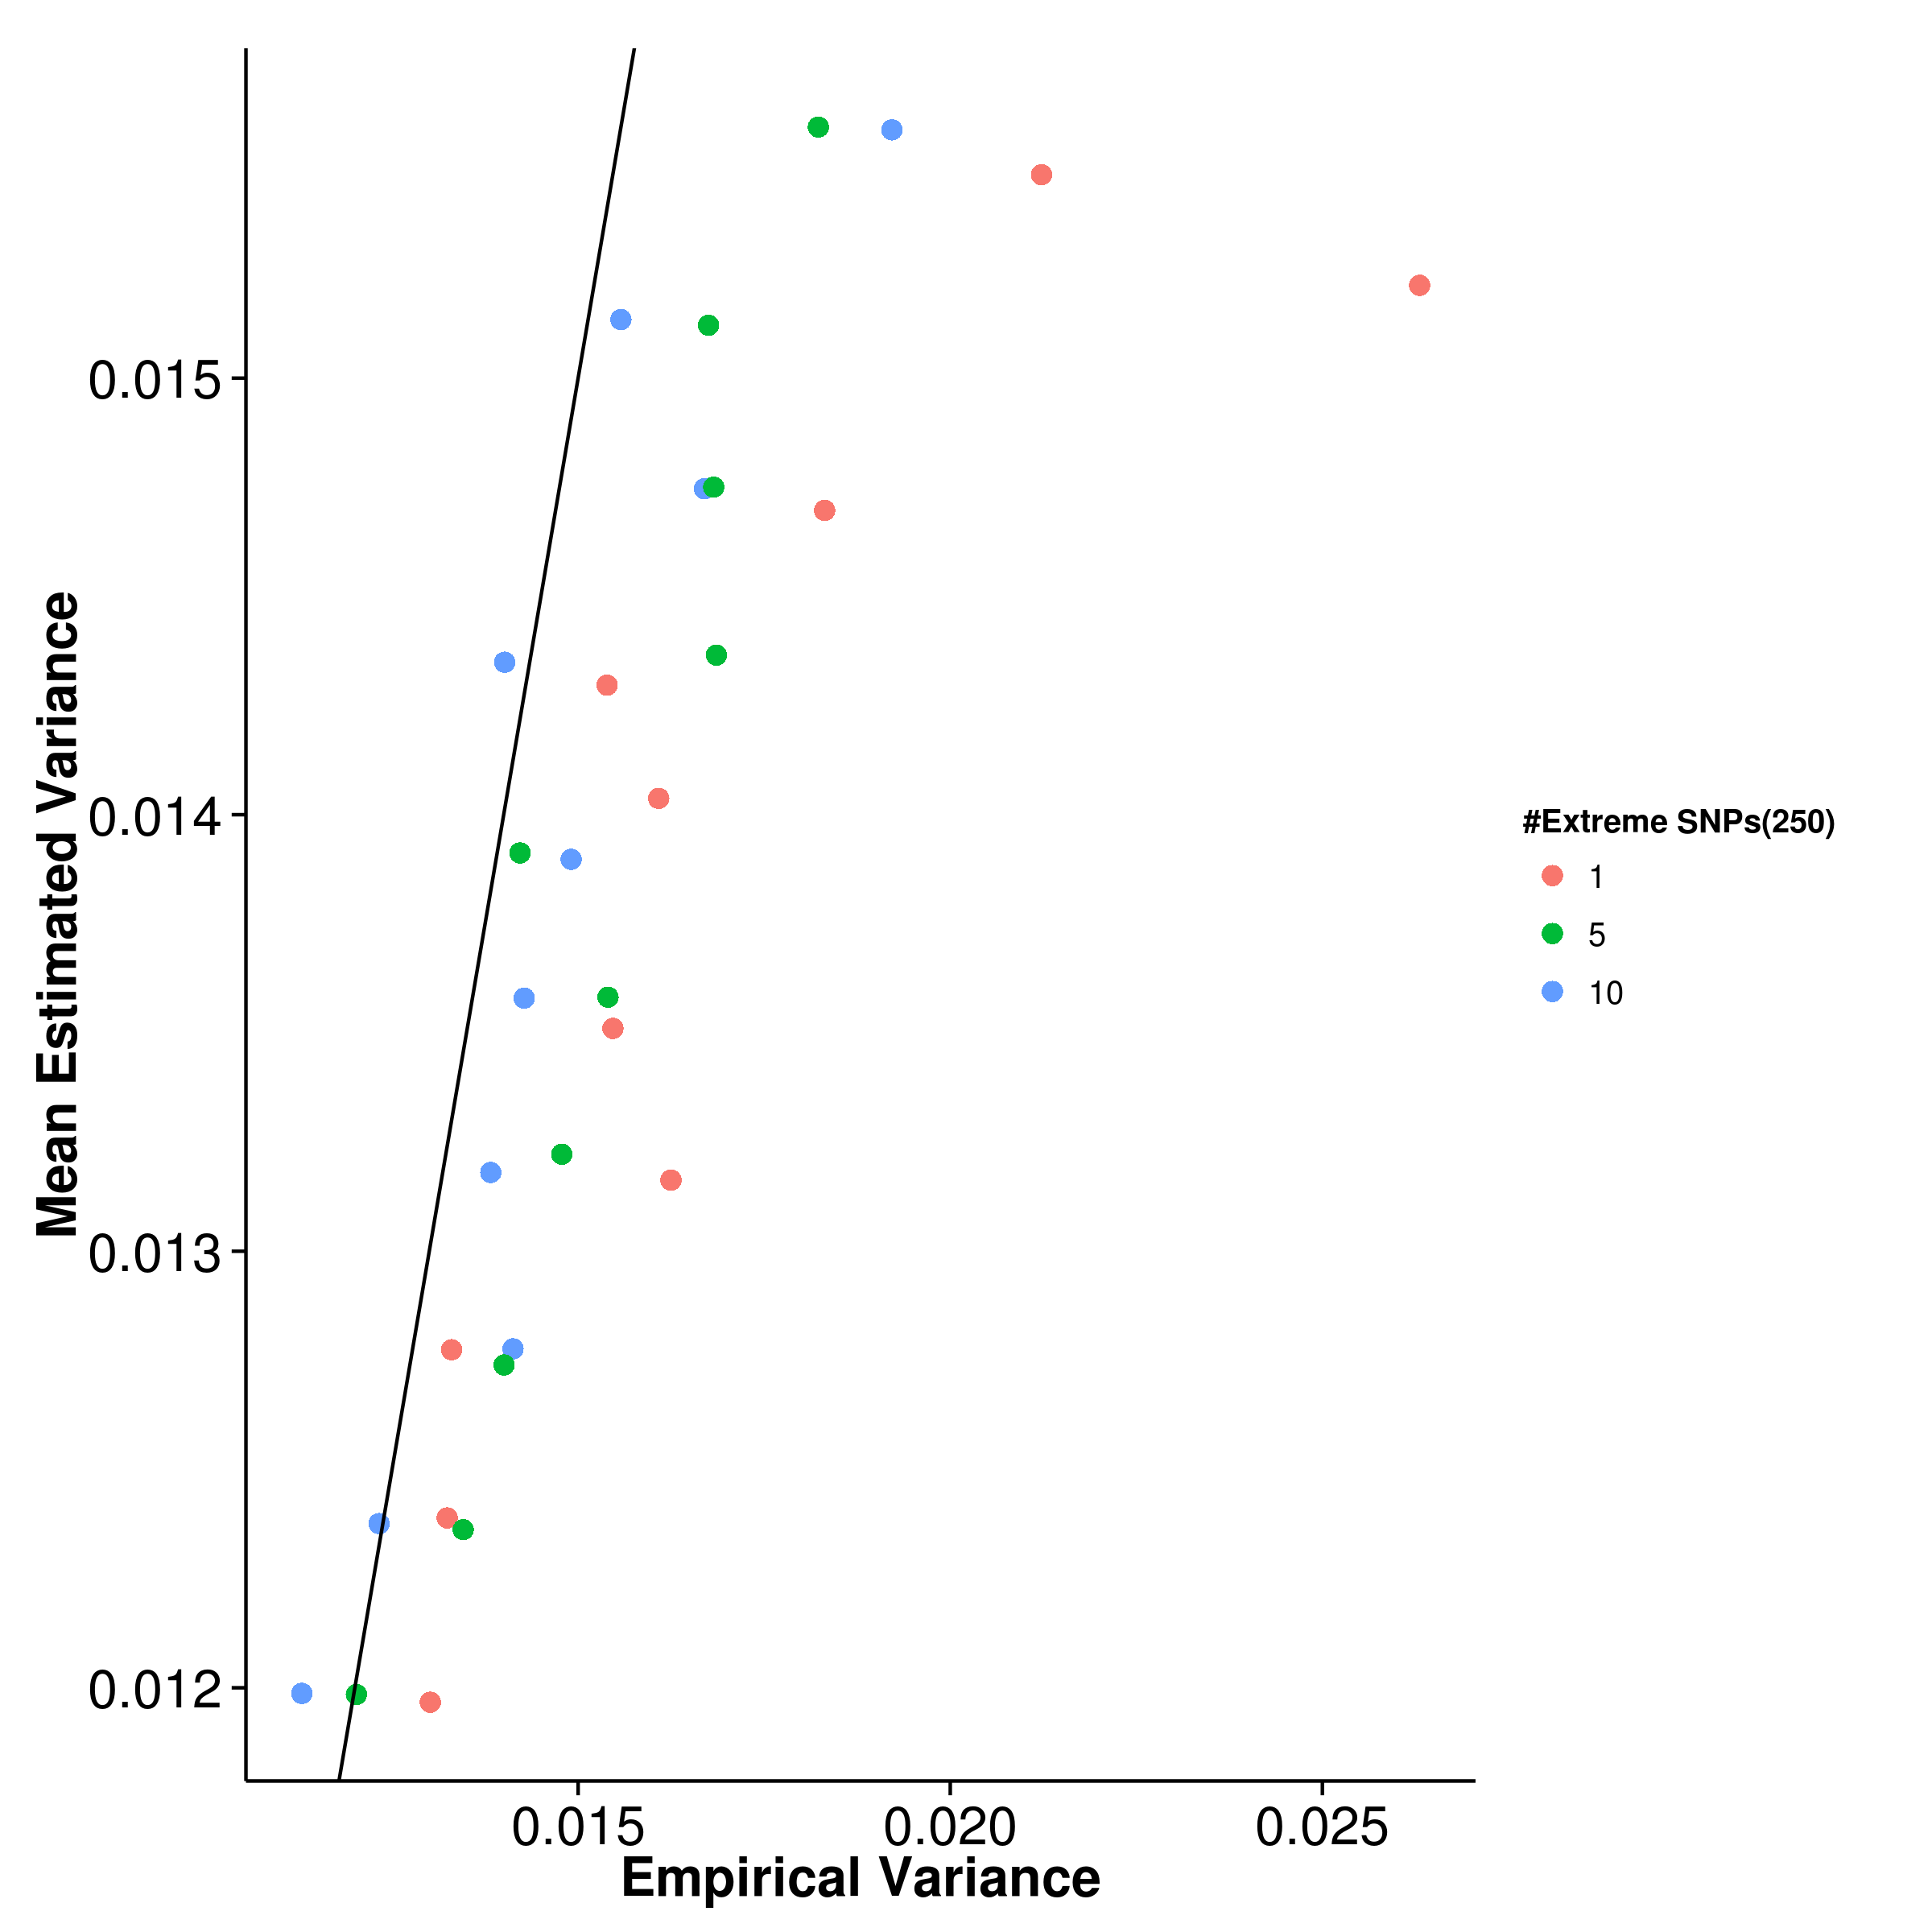
\includegraphics{figure/he_summary/extreme_250c/shrek_QtE_Extreme_sdCom.png}}
				\label{fig:shrekQtEx250cVarCom}
			}
			\subfloat[GCTA]{
				\scalebox{.4}{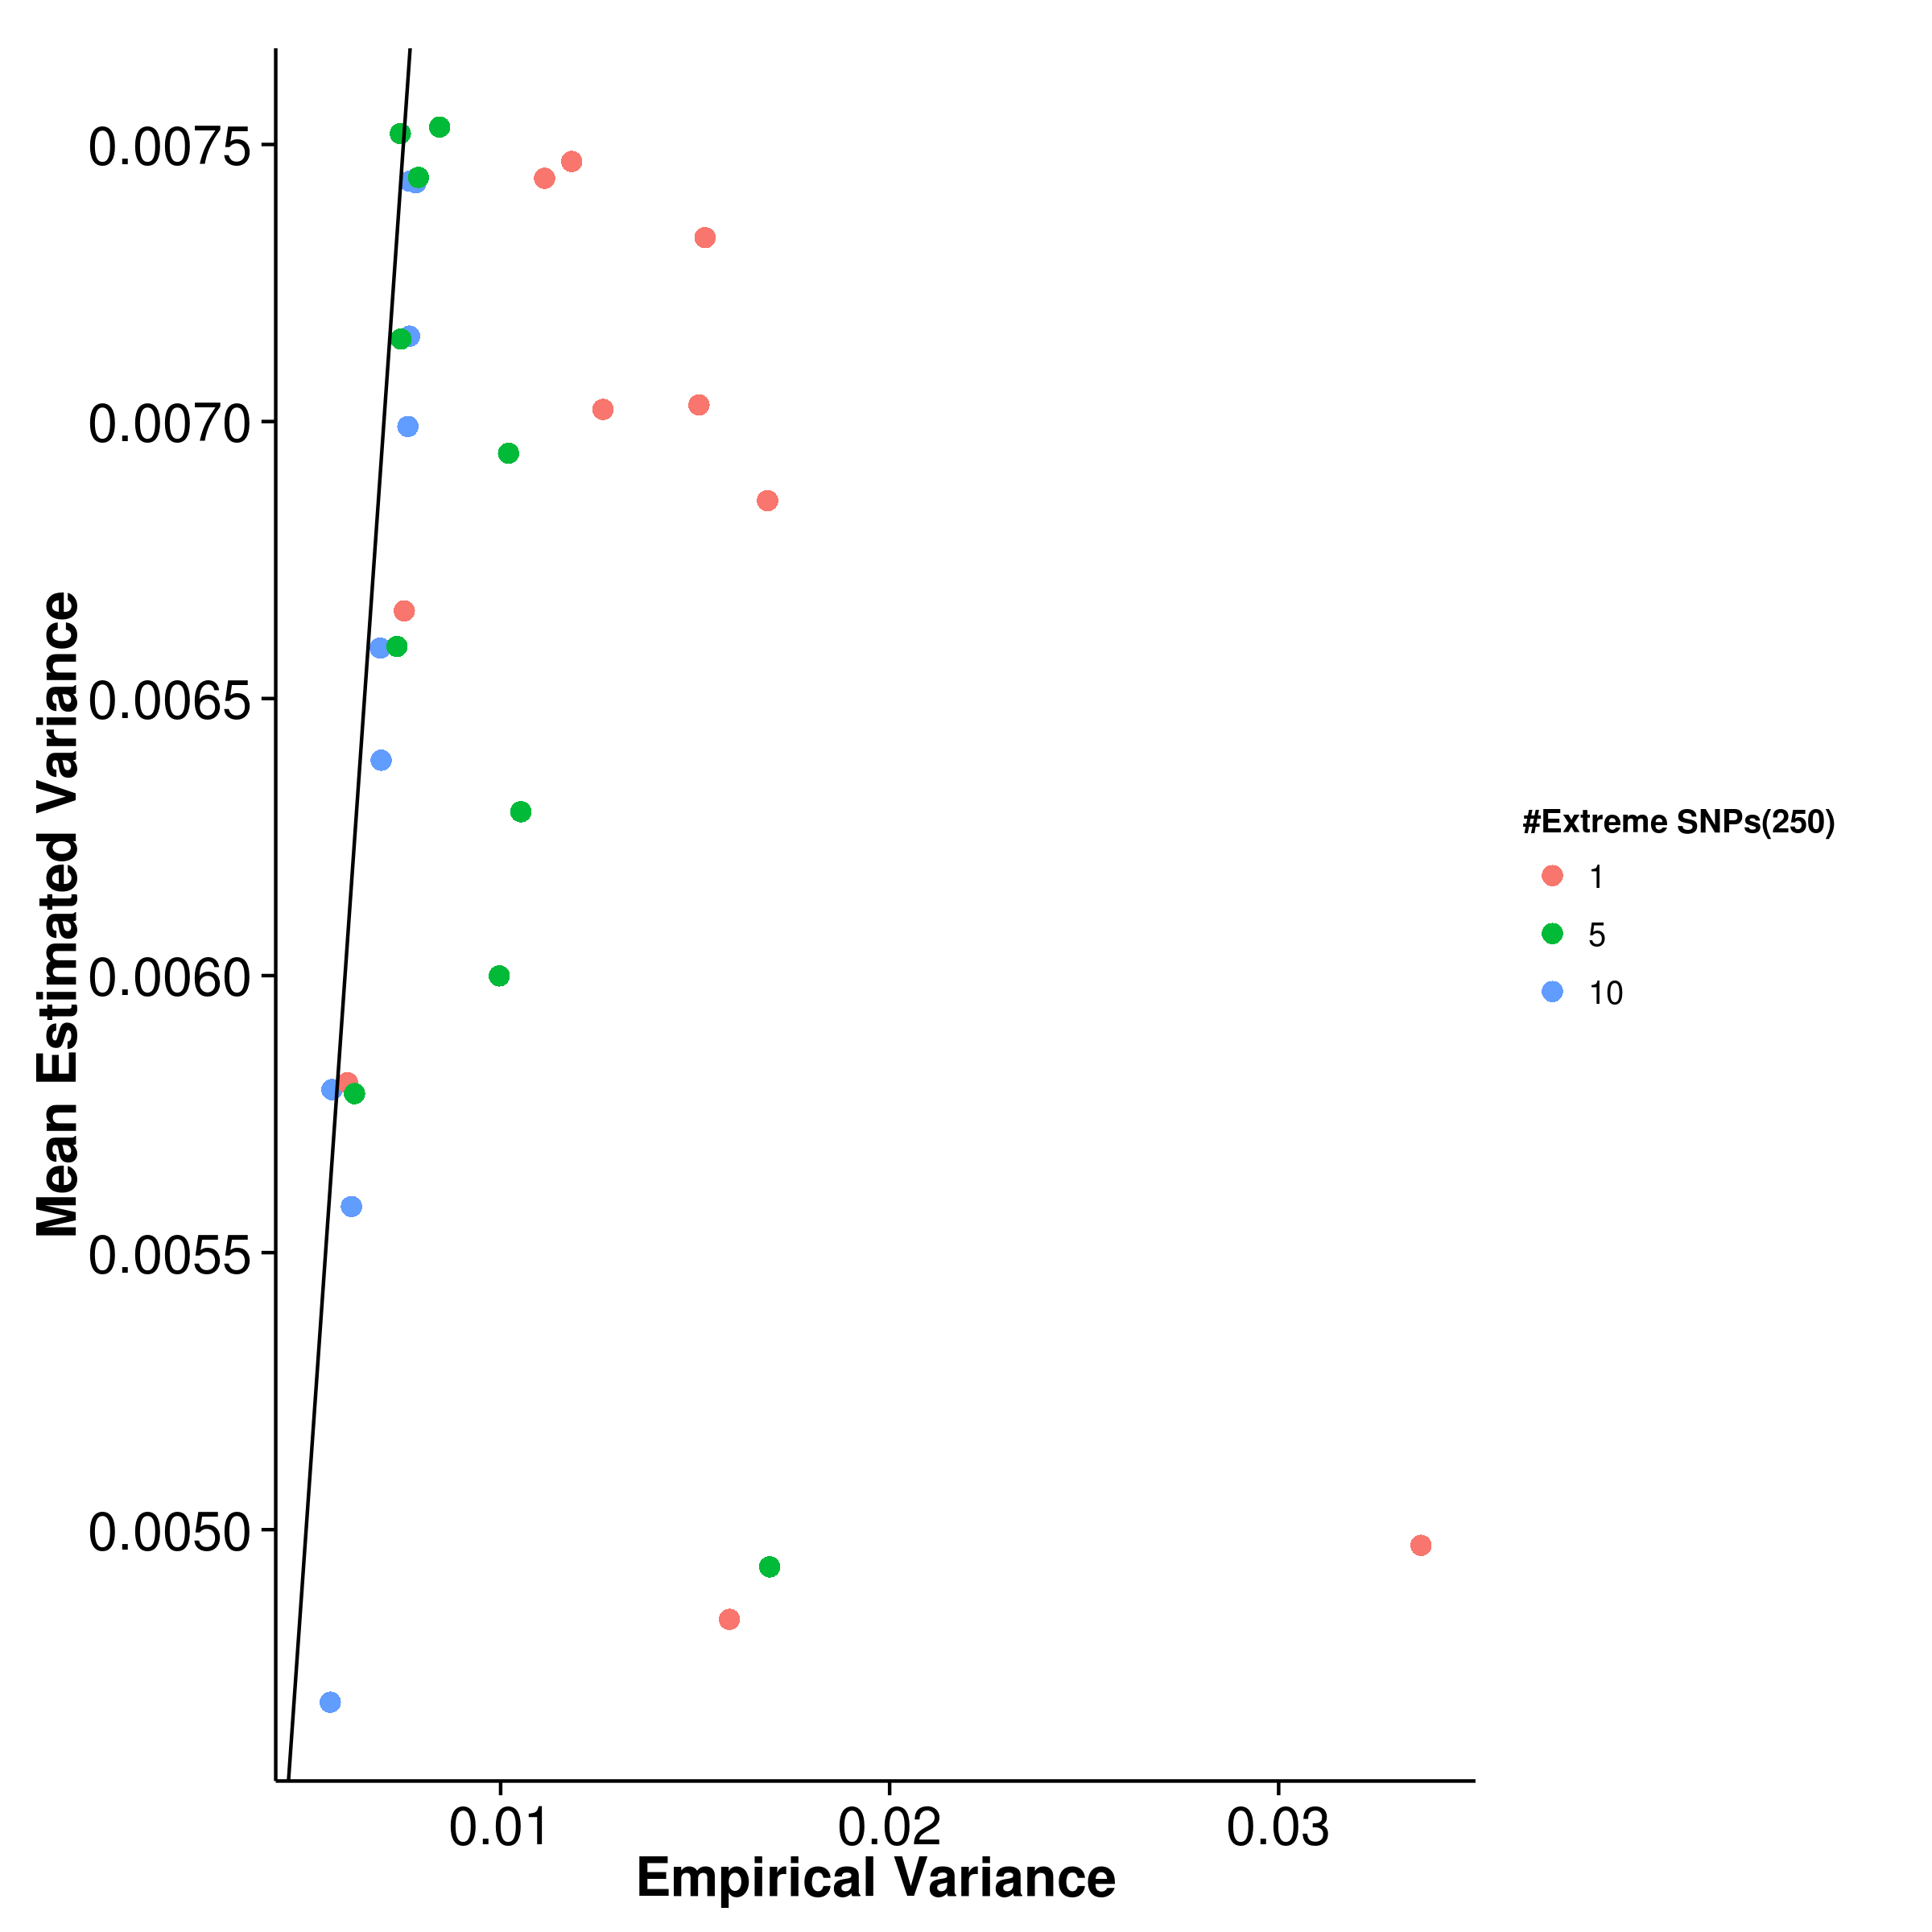
\includegraphics{figure/he_summary/extreme_250c/gcta_QtE_Extreme_sdCom.png}}
				\label{fig:gctaQtEx250cVarCom}
			}\\
			\subfloat[LDSC with fix intercept]{
				\scalebox{.4}{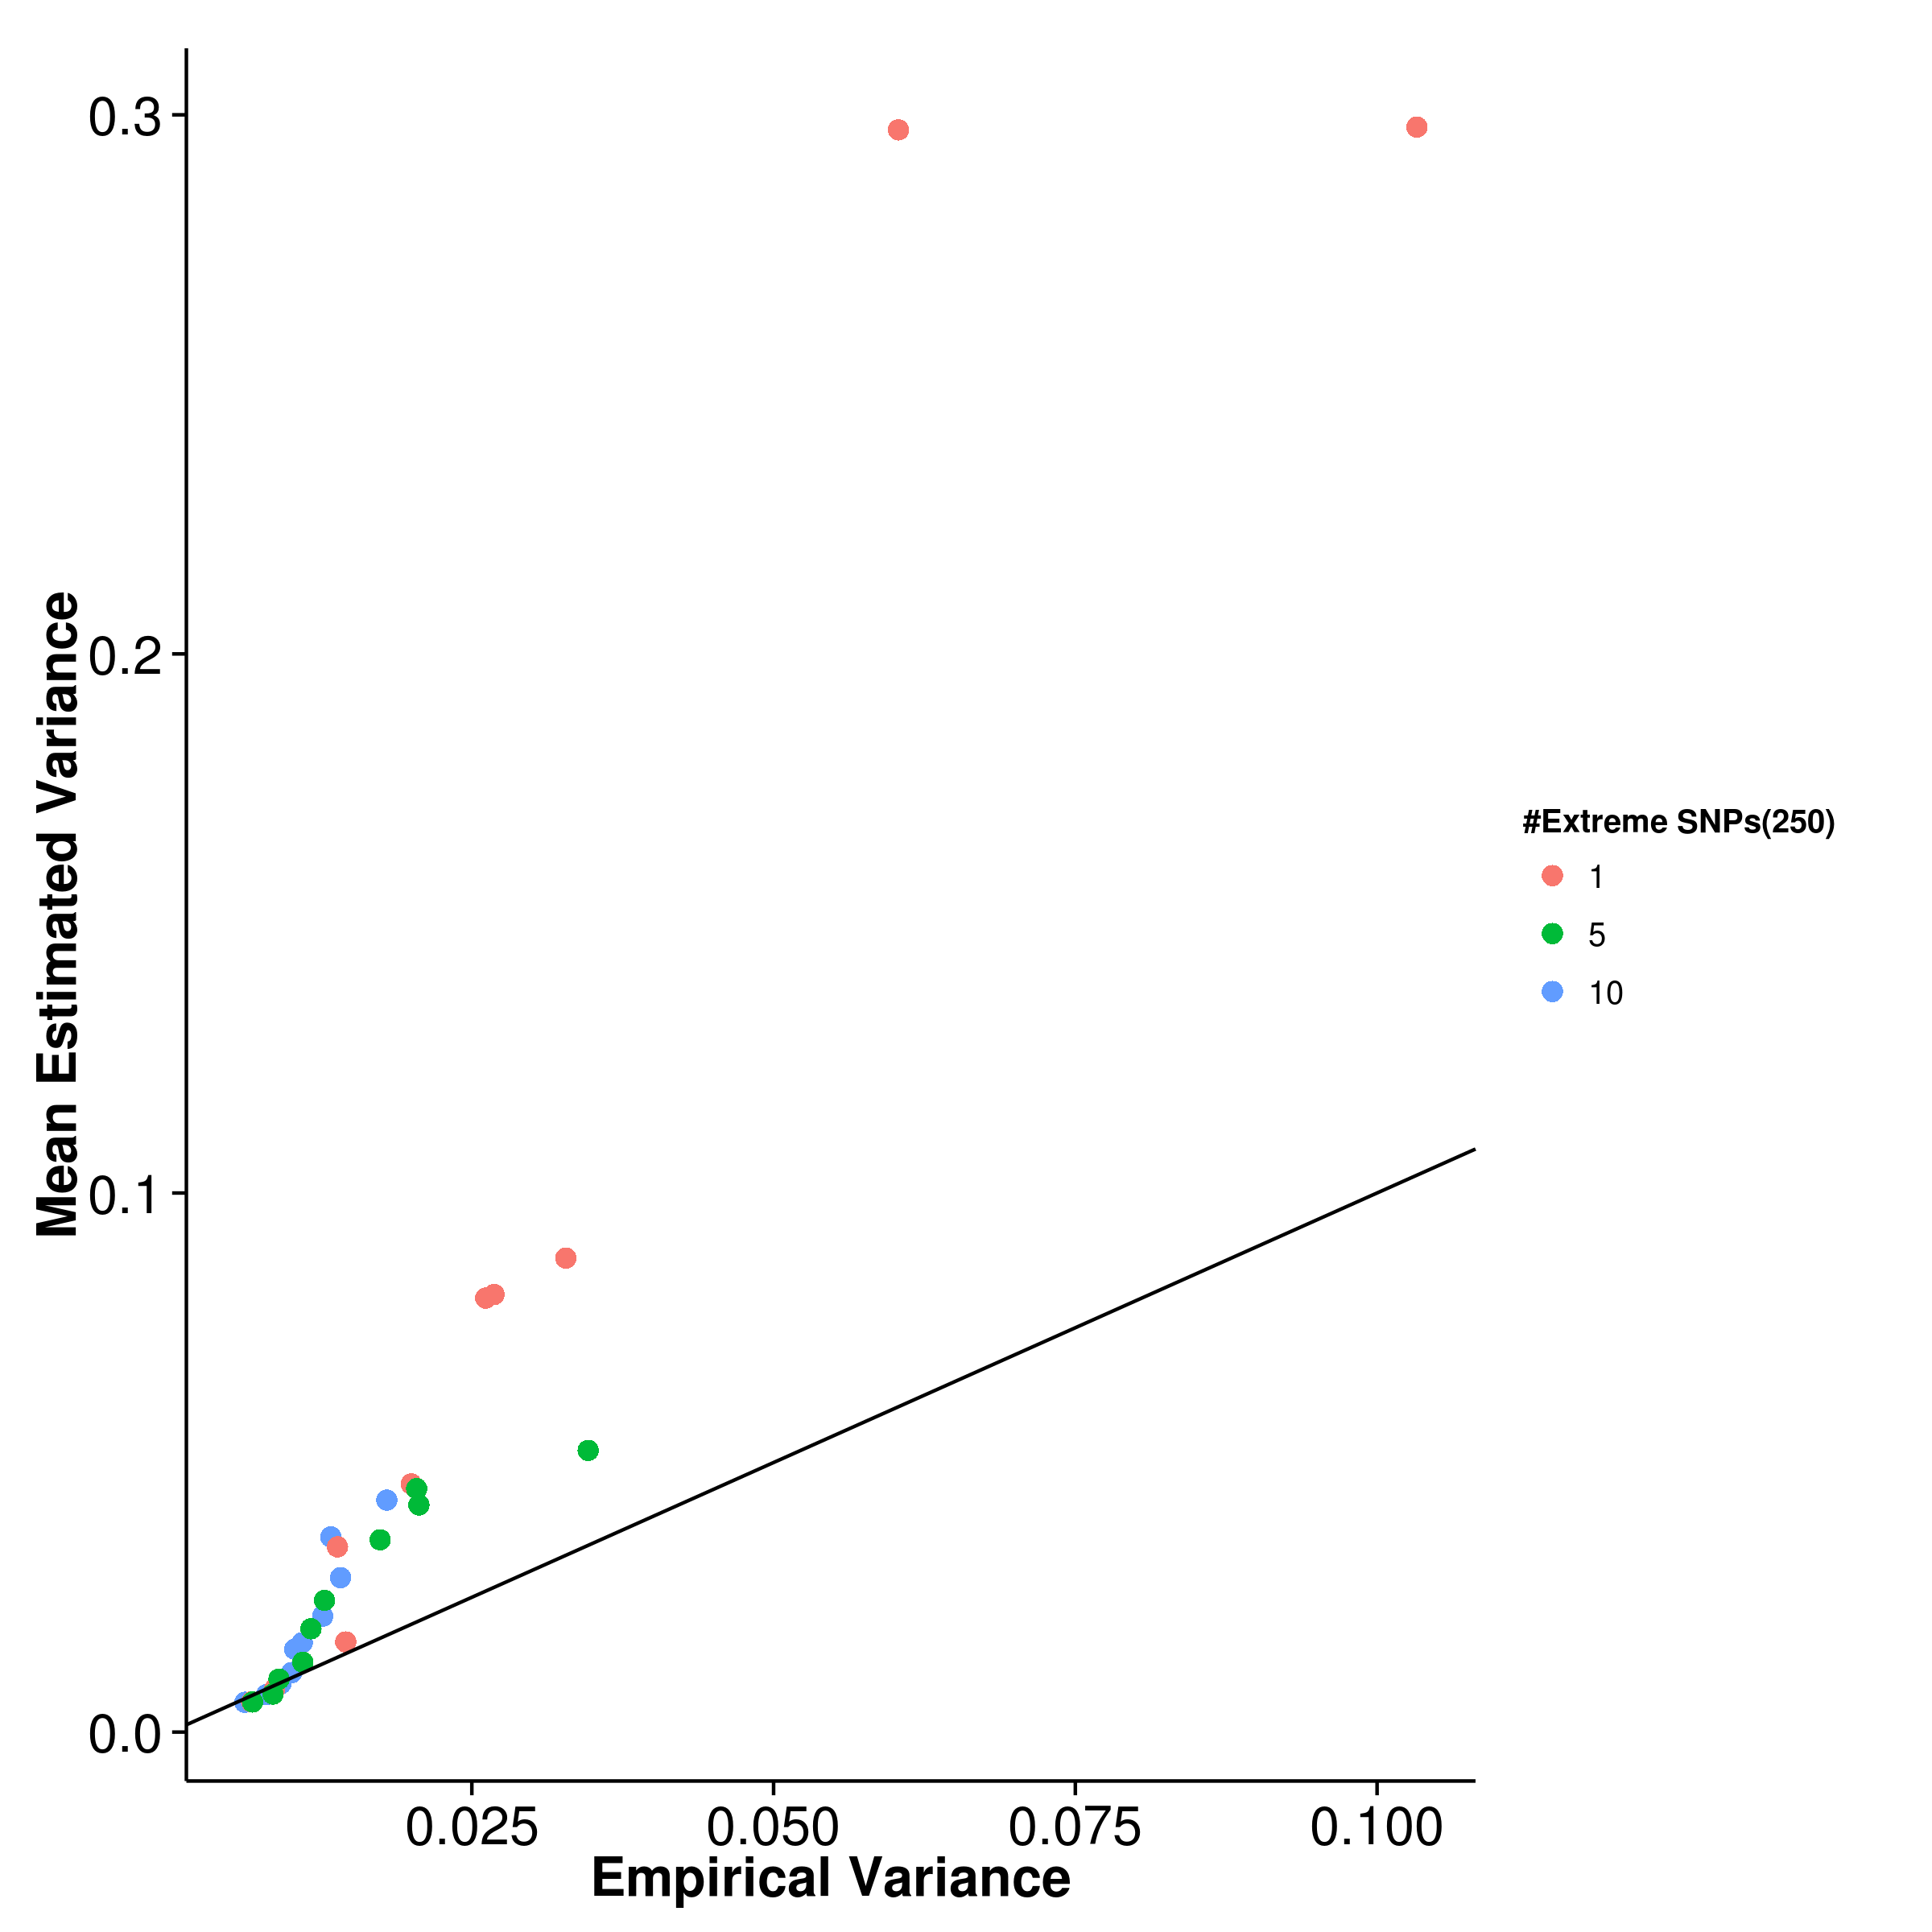
\includegraphics{figure/he_summary/extreme_250c/ldsc_QtE_Extreme_sdCom.png}}
				\label{fig:ldscQtEx250cVarCom}
			}
			\subfloat[LDSC with intercept estimation]{
				
				\scalebox{.4}{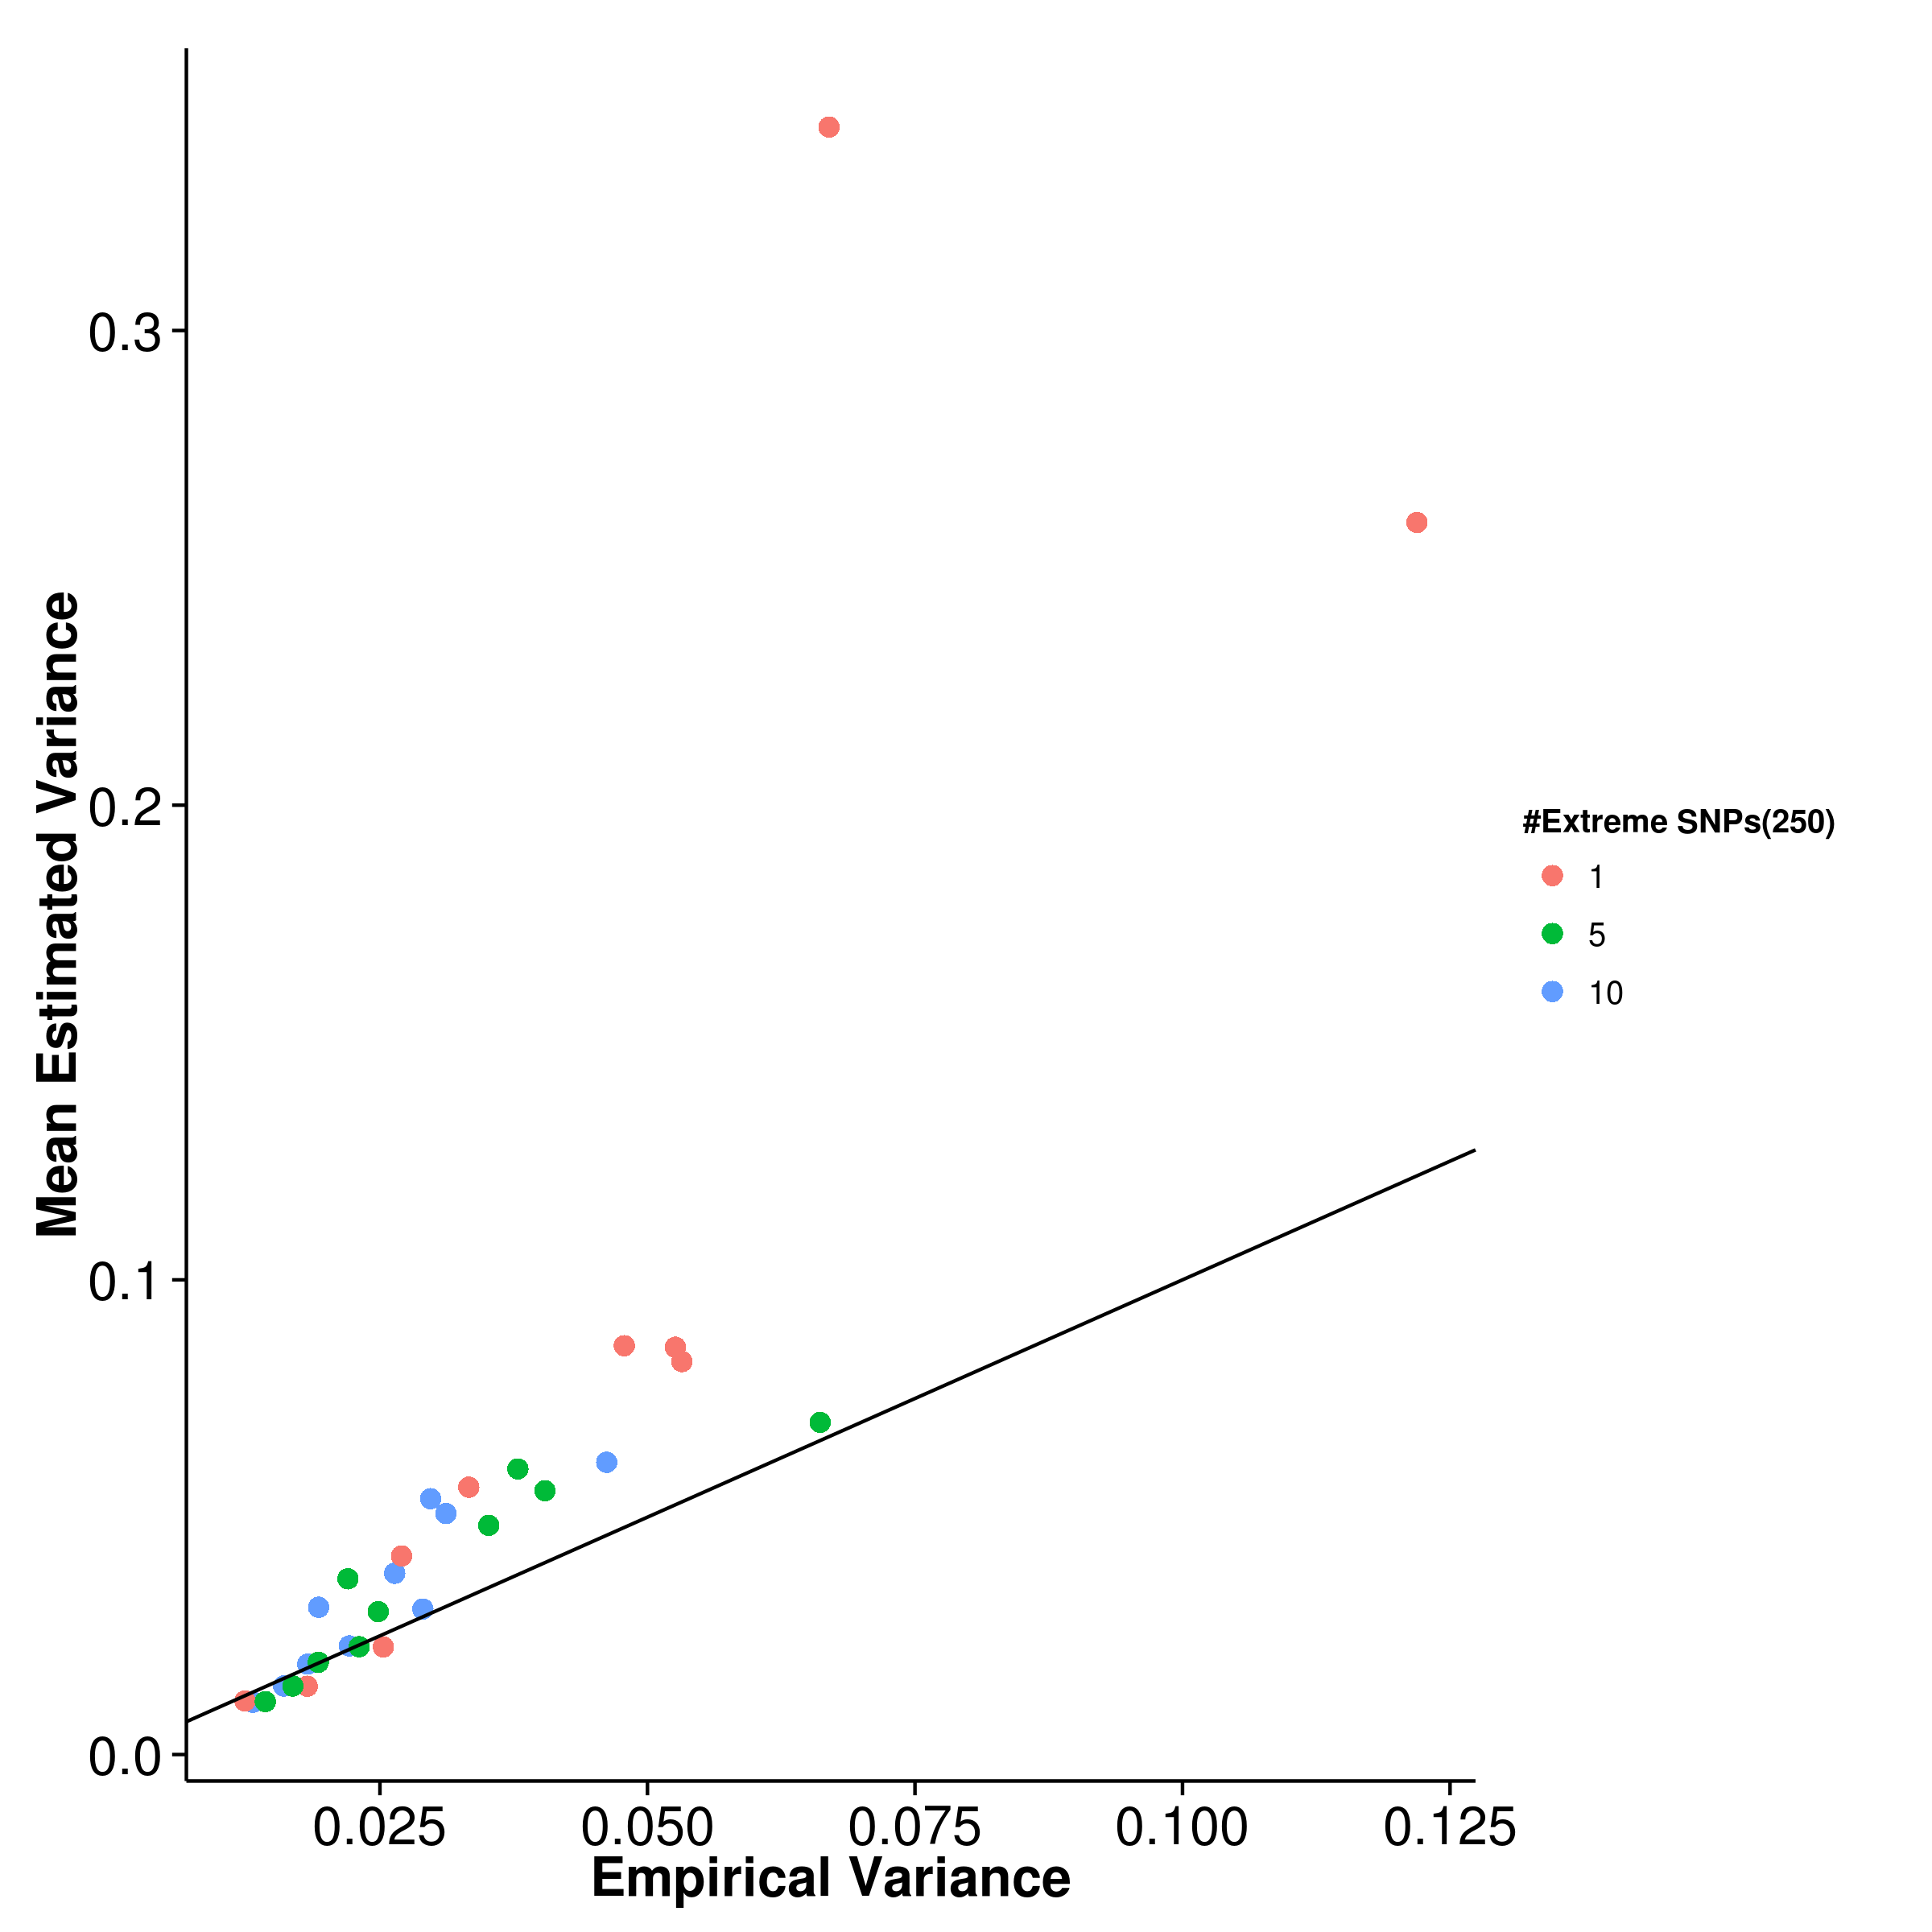
\includegraphics{figure/he_summary/extreme_250c/ldscIn_QtE_Extreme_sdCom.png}}
				\label{fig:ldscInQtEx250cVarCom}
			}
			\caption[Quantitative Trait with Extreme Effect Size Simulation Result(250 causal SNPs, Estimated Variance)]
			{Estimated variance of results from quantitative trait simulation with extreme effect size simulation when compared to the empirical variance.
				250 causal \glspl{SNP} were simulated.
				The result of simulation were the same as the previous extreme effect simulation with 100 causal \glspl{SNP}.
			} 
			\label{fig:QtEx250cVarCom}
		\end{figure}
		% CC Rand Effect
		\subsection{Case Control Simulation}
		\begin{figure}
			\centering
			\subfloat[SHREK]{
				\scalebox{.4}{\includegraphics{figure/he_summary/cc_100c/shrek_CC_Random_mean.png}}
				\label{fig:shrekCCRandMean}
			}
			\subfloat[GCTA]{
				\scalebox{.4}{\includegraphics{figure/he_summary/cc_100c/gcta_CC_Random_mean.png}}
				\label{fig:gctaCCRandMean}
			}\\
			\subfloat[LDSC with fix intercept]{
				\scalebox{.4}{\includegraphics{figure/he_summary/cc_100c/ldsc_CC_Random_mean.png}}
				\label{fig:ldscCCRandMean}
			}
			\subfloat[LDSC with intercept estimation]{
				
				\scalebox{.4}{\includegraphics{figure/he_summary/cc_100c/ldscIn_CC_Random_mean.png}}
				\label{fig:ldscInCCRandMean}
			}
			\caption[Case Control with Random Effect Size Simulation Result(Mean)]
			{Mean of results from case control simulation with random effect size simulation.
				The performance of \gls{gcta} was as suggested by \citet{Golan2014} where there was an underestimation as prevalence decreases.
				On the other hand, \gls{ldsc} were upwardly biased when a fixed intercept was used and this bias was corrected when an estimation of intercept was allowed.
				\gls{shrek} does not seems to as sensitive to change in prevalence and the estimation were relatively robust.
				} 
			\label{fig:CCRandMean}
		\end{figure}
		
		\begin{figure}
			\centering
			\subfloat[SHREK]{
				\scalebox{.4}{\includegraphics{figure/he_summary/cc_100c/shrek_CC_Random_sd.png}}
				\label{fig:shrekCCRandVar}
			}
			\subfloat[GCTA]{
				\scalebox{.4}{\includegraphics{figure/he_summary/cc_100c/gcta_CC_Random_sd.png}}
				\label{fig:gctaCCRandVar}
			}\\
			\subfloat[LDSC with fix intercept]{
				\scalebox{.4}{\includegraphics{figure/he_summary/cc_100c/ldsc_CC_Random_sd.png}}
				\label{fig:ldscCCRandVar}
			}
			\subfloat[LDSC with intercept estimation]{
				
				\scalebox{.4}{\includegraphics{figure/he_summary/cc_100c/ldscIn_CC_Random_sd.png}}
				\label{fig:ldscInCCRandVar}
			}
			\caption[Case Control with Random Effect Size Simulation Result(Variance)]
			{Variance of results from case control simulation with random effect size simulation.
				It was clear that the prevalence affects the variance of estimation where a larger variance tends to increase the variance of estimation.
				Again, \gls{gcta} has the lowest variance, however, unlike in the quantitative trait simulation, \gls{shrek} has a lower average variance when compared to \gls{ldsc} with fixed intercept.
				Nonetheless, it was important to remember that in case control simulation, a much smaller amount of \glspl{SNP} was used, thus the results was not directly comparable to results from the quantitative simulation.
			} 
			\label{fig:CCRandVar}
		\end{figure}
		
		
		\begin{figure}
			\centering
			\subfloat[SHREK]{
				\scalebox{.4}{\includegraphics{figure/he_summary/cc_100c/shrek_CC_Random_sdCom.png}}
				\label{fig:shrekCCRandVarCom}
			}
			\subfloat[GCTA]{
				\scalebox{.4}{\includegraphics{figure/he_summary/cc_100c/gcta_CC_Random_sdCom.png}}
				\label{fig:gctaCCRandVarCom}
			}\\
			\subfloat[LDSC with fix intercept]{
				\scalebox{.4}{\includegraphics{figure/he_summary/cc_100c/ldsc_CC_Random_sdCom.png}}
				\label{fig:ldscCCRandVarCom}
			}
			\subfloat[LDSC with intercept estimation]{
				
				\scalebox{.4}{\includegraphics{figure/he_summary/cc_100c/ldscIn_CC_Random_sdCom.png}}
				\label{fig:ldscInCCRandVarCom}
			}
			\caption[Case Control with Random Effect Size Simulation Result(Estimated Variance)]
			{Estimated variance of results from case control simulation with random effect size simulation when compared to empirical variance.
				From the quantitative trait simulation with random effect size(\cref{fig:QtRandVarCom}), it was observed that the variance estimation of \gls{shrek} and \gls{gcta} were rater accurate.
				Similarly, in the case control simulation with 100 causal \glspl{SNP}, it was observed that the variance estimation of \gls{shrek} and \gls{gcta} were close to the empirical variance with slight bias.
				A large up-ward bias was observed for \gls{ldsc} with fixed intercept estimation but the bias was less when \gls{ldsc} was allowed to estimate the intercept.s
			} 
			\label{fig:CCRandVarCom}
		\end{figure}
		
		
		
		
	\section{Discussion}
	
	\section{Supplementary place holder}
	
	%Put these graphs in supplementary instead